\documentclass[twoside]{book}

% Packages required by doxygen
\usepackage{fixltx2e}
\usepackage{calc}
\usepackage{doxygen}
\usepackage[export]{adjustbox} % also loads graphicx
\usepackage{graphicx}
\usepackage[utf8]{inputenc}
\usepackage{makeidx}
\usepackage{multicol}
\usepackage{multirow}
\PassOptionsToPackage{warn}{textcomp}
\usepackage{textcomp}
\usepackage[nointegrals]{wasysym}
\usepackage[table]{xcolor}

% Font selection
\usepackage[T1]{fontenc}
\usepackage[scaled=.90]{helvet}
\usepackage{courier}
\usepackage{amssymb}
\usepackage{sectsty}
\renewcommand{\familydefault}{\sfdefault}
\allsectionsfont{%
  \fontseries{bc}\selectfont%
  \color{darkgray}%
}
\renewcommand{\DoxyLabelFont}{%
  \fontseries{bc}\selectfont%
  \color{darkgray}%
}
\newcommand{\+}{\discretionary{\mbox{\scriptsize$\hookleftarrow$}}{}{}}

% Page & text layout
\usepackage{geometry}
\geometry{%
  a4paper,%
  top=2.5cm,%
  bottom=2.5cm,%
  left=2.5cm,%
  right=2.5cm%
}
\tolerance=750
\hfuzz=15pt
\hbadness=750
\setlength{\emergencystretch}{15pt}
\setlength{\parindent}{0cm}
\setlength{\parskip}{3ex plus 2ex minus 2ex}
\makeatletter
\renewcommand{\paragraph}{%
  \@startsection{paragraph}{4}{0ex}{-1.0ex}{1.0ex}{%
    \normalfont\normalsize\bfseries\SS@parafont%
  }%
}
\renewcommand{\subparagraph}{%
  \@startsection{subparagraph}{5}{0ex}{-1.0ex}{1.0ex}{%
    \normalfont\normalsize\bfseries\SS@subparafont%
  }%
}
\makeatother

% Headers & footers
\usepackage{fancyhdr}
\pagestyle{fancyplain}
\fancyhead[LE]{\fancyplain{}{\bfseries\thepage}}
\fancyhead[CE]{\fancyplain{}{}}
\fancyhead[RE]{\fancyplain{}{\bfseries\leftmark}}
\fancyhead[LO]{\fancyplain{}{\bfseries\rightmark}}
\fancyhead[CO]{\fancyplain{}{}}
\fancyhead[RO]{\fancyplain{}{\bfseries\thepage}}
\fancyfoot[LE]{\fancyplain{}{}}
\fancyfoot[CE]{\fancyplain{}{}}
\fancyfoot[RE]{\fancyplain{}{\bfseries\scriptsize Generated by Doxygen }}
\fancyfoot[LO]{\fancyplain{}{\bfseries\scriptsize Generated by Doxygen }}
\fancyfoot[CO]{\fancyplain{}{}}
\fancyfoot[RO]{\fancyplain{}{}}
\renewcommand{\footrulewidth}{0.4pt}
\renewcommand{\chaptermark}[1]{%
  \markboth{#1}{}%
}
\renewcommand{\sectionmark}[1]{%
  \markright{\thesection\ #1}%
}

% Indices & bibliography
\usepackage{natbib}
\usepackage[titles]{tocloft}
\setcounter{tocdepth}{3}
\setcounter{secnumdepth}{5}
\makeindex

% Hyperlinks (required, but should be loaded last)
\usepackage{ifpdf}
\ifpdf
  \usepackage[pdftex,pagebackref=true]{hyperref}
\else
  \usepackage[ps2pdf,pagebackref=true]{hyperref}
\fi
\hypersetup{%
  colorlinks=true,%
  linkcolor=blue,%
  citecolor=blue,%
  unicode%
}

% Custom commands
\newcommand{\clearemptydoublepage}{%
  \newpage{\pagestyle{empty}\cleardoublepage}%
}

\usepackage{caption}
\captionsetup{labelsep=space,justification=centering,font={bf},singlelinecheck=off,skip=4pt,position=top}

%===== C O N T E N T S =====

\begin{document}

% Titlepage & ToC
\hypersetup{pageanchor=false,
             bookmarksnumbered=true,
             pdfencoding=unicode
            }
\pagenumbering{alph}
\begin{titlepage}
\vspace*{7cm}
\begin{center}%
{\Large Q\+Rail }\\
\vspace*{1cm}
{\large Generated by Doxygen 1.8.14}\\
\end{center}
\end{titlepage}
\clearemptydoublepage
\pagenumbering{roman}
\tableofcontents
\clearemptydoublepage
\pagenumbering{arabic}
\hypersetup{pageanchor=true}

%--- Begin generated contents ---
\chapter{Namespace Index}
\section{Namespace List}
Here is a list of all namespaces with brief descriptions\+:\begin{DoxyCompactList}
\item\contentsline{section}{\mbox{\hyperlink{namespaceAlertsEngine}{Alerts\+Engine}} \\*Sets the description of the message to the given Q\+String \&description }{\pageref{namespaceAlertsEngine}}{}
\item\contentsline{section}{\mbox{\hyperlink{namespaceLiveboard}{Liveboard}} \\*Retrieves a liveboard by a station U\+RI and a time range }{\pageref{namespaceLiveboard}}{}
\item\contentsline{section}{\mbox{\hyperlink{namespaceNetwork}{Network}} \\*Constructs a \mbox{\hyperlink{classQRail_1_1Network_1_1Manager}{Q\+Rail\+::\+Network\+::\+Manager}} facade to access the network using the H\+T\+TP protocol }{\pageref{namespaceNetwork}}{}
\item\contentsline{section}{\mbox{\hyperlink{namespaceQRail}{Q\+Rail}} }{\pageref{namespaceQRail}}{}
\item\contentsline{section}{\mbox{\hyperlink{namespaceQRail_1_1AlertsEngine}{Q\+Rail\+::\+Alerts\+Engine}} }{\pageref{namespaceQRail_1_1AlertsEngine}}{}
\item\contentsline{section}{\mbox{\hyperlink{namespaceQRail_1_1Database}{Q\+Rail\+::\+Database}} }{\pageref{namespaceQRail_1_1Database}}{}
\item\contentsline{section}{\mbox{\hyperlink{namespaceQRail_1_1Fragments}{Q\+Rail\+::\+Fragments}} }{\pageref{namespaceQRail_1_1Fragments}}{}
\item\contentsline{section}{\mbox{\hyperlink{namespaceQRail_1_1LiveboardEngine}{Q\+Rail\+::\+Liveboard\+Engine}} }{\pageref{namespaceQRail_1_1LiveboardEngine}}{}
\item\contentsline{section}{\mbox{\hyperlink{namespaceQRail_1_1Network}{Q\+Rail\+::\+Network}} }{\pageref{namespaceQRail_1_1Network}}{}
\item\contentsline{section}{\mbox{\hyperlink{namespaceQRail_1_1RouterEngine}{Q\+Rail\+::\+Router\+Engine}} }{\pageref{namespaceQRail_1_1RouterEngine}}{}
\item\contentsline{section}{\mbox{\hyperlink{namespaceQRail_1_1StationEngine}{Q\+Rail\+::\+Station\+Engine}} }{\pageref{namespaceQRail_1_1StationEngine}}{}
\item\contentsline{section}{\mbox{\hyperlink{namespaceQRail_1_1VehicleEngine}{Q\+Rail\+::\+Vehicle\+Engine}} }{\pageref{namespaceQRail_1_1VehicleEngine}}{}
\item\contentsline{section}{\mbox{\hyperlink{namespaceRouterEngine}{Router\+Engine}} \\*Constructs a Route with a list of legs and transfers }{\pageref{namespaceRouterEngine}}{}
\item\contentsline{section}{\mbox{\hyperlink{namespaceStationEngine}{Station\+Engine}} \\*Retrieves a vehicle by U\+RI from the network i\+Rail A\+PI }{\pageref{namespaceStationEngine}}{}
\item\contentsline{section}{\mbox{\hyperlink{namespaceVehicleEngine}{Vehicle\+Engine}} \\*Constructs a \mbox{\hyperlink{classQRail_1_1VehicleEngine_1_1Factory}{Q\+Rail\+::\+Vehicle\+Engine\+::\+Factory}} to generate \mbox{\hyperlink{classQRail_1_1VehicleEngine_1_1Vehicle}{Q\+Rail\+::\+Vehicle\+Engine\+::\+Vehicle}} objects on the fly }{\pageref{namespaceVehicleEngine}}{}
\end{DoxyCompactList}

\chapter{Hierarchical Index}
\section{Class Hierarchy}
This inheritance list is sorted roughly, but not completely, alphabetically\+:\begin{DoxyCompactList}
\item Q\+Object\begin{DoxyCompactList}
\item \contentsline{section}{Alerts\+Engine\+:\+:Message}{\pageref{classAlertsEngine_1_1Message}}{}
\item \contentsline{section}{Database\+:\+:Manager}{\pageref{classDatabase_1_1Manager}}{}
\item \contentsline{section}{Fragments\+:\+:Factory}{\pageref{classFragments_1_1Factory}}{}
\item \contentsline{section}{Fragments\+:\+:Fragment}{\pageref{classFragments_1_1Fragment}}{}
\item \contentsline{section}{Fragments\+:\+:Page}{\pageref{classFragments_1_1Page}}{}
\item \contentsline{section}{Liveboard\+Engine\+:\+:Board}{\pageref{classLiveboardEngine_1_1Board}}{}
\item \contentsline{section}{Liveboard\+Engine\+:\+:Factory}{\pageref{classLiveboardEngine_1_1Factory}}{}
\item \contentsline{section}{Network\+:\+:Manager}{\pageref{classNetwork_1_1Manager}}{}
\item \contentsline{section}{OS}{\pageref{classOS}}{}
\item \contentsline{section}{Router\+Engine\+:\+:Planner}{\pageref{classRouterEngine_1_1Planner}}{}
\item \contentsline{section}{Router\+Engine\+:\+:Route}{\pageref{classRouterEngine_1_1Route}}{}
\item \contentsline{section}{Router\+Engine\+:\+:Route\+Leg}{\pageref{classRouterEngine_1_1RouteLeg}}{}
\item \contentsline{section}{Router\+Engine\+:\+:Route\+Leg\+End}{\pageref{classRouterEngine_1_1RouteLegEnd}}{}
\item \contentsline{section}{Router\+Engine\+:\+:Station\+Stop\+Profile}{\pageref{classRouterEngine_1_1StationStopProfile}}{}
\item \contentsline{section}{Router\+Engine\+:\+:Train\+Profile}{\pageref{classRouterEngine_1_1TrainProfile}}{}
\item \contentsline{section}{Router\+Engine\+:\+:Transfer}{\pageref{classRouterEngine_1_1Transfer}}{}
\item \contentsline{section}{Station\+Engine\+:\+:Factory}{\pageref{classStationEngine_1_1Factory}}{}
\item \contentsline{section}{Station\+Engine\+:\+:Station}{\pageref{classStationEngine_1_1Station}}{}
\begin{DoxyCompactList}
\item \contentsline{section}{Station\+Engine\+:\+:Null\+Station}{\pageref{classStationEngine_1_1NullStation}}{}
\end{DoxyCompactList}
\item \contentsline{section}{Vehicle\+Engine\+:\+:Factory}{\pageref{classVehicleEngine_1_1Factory}}{}
\item \contentsline{section}{Vehicle\+Engine\+:\+:Stop}{\pageref{classVehicleEngine_1_1Stop}}{}
\item \contentsline{section}{Vehicle\+Engine\+:\+:Vehicle}{\pageref{classVehicleEngine_1_1Vehicle}}{}
\end{DoxyCompactList}
\end{DoxyCompactList}

\chapter{Data Structure Index}
\section{Data Structures}
Here are the data structures with brief descriptions\+:\begin{DoxyCompactList}
\item\contentsline{section}{\mbox{\hyperlink{classQRail_1_1LiveboardEngine_1_1Board}{Q\+Rail\+::\+Liveboard\+Engine\+::\+Board}} }{\pageref{classQRail_1_1LiveboardEngine_1_1Board}}{}
\item\contentsline{section}{\mbox{\hyperlink{classQRail_1_1Fragments_1_1Dispatcher}{Q\+Rail\+::\+Fragments\+::\+Dispatcher}} }{\pageref{classQRail_1_1Fragments_1_1Dispatcher}}{}
\item\contentsline{section}{\mbox{\hyperlink{classQRail_1_1Network_1_1Dispatcher}{Q\+Rail\+::\+Network\+::\+Dispatcher}} }{\pageref{classQRail_1_1Network_1_1Dispatcher}}{}
\item\contentsline{section}{\mbox{\hyperlink{classQRail_1_1Fragments_1_1DispatcherEvent}{Q\+Rail\+::\+Fragments\+::\+Dispatcher\+Event}} }{\pageref{classQRail_1_1Fragments_1_1DispatcherEvent}}{}
\item\contentsline{section}{\mbox{\hyperlink{classQRail_1_1Network_1_1DispatcherEvent}{Q\+Rail\+::\+Network\+::\+Dispatcher\+Event}} }{\pageref{classQRail_1_1Network_1_1DispatcherEvent}}{}
\item\contentsline{section}{\mbox{\hyperlink{classQRail_1_1VehicleEngine_1_1Factory}{Q\+Rail\+::\+Vehicle\+Engine\+::\+Factory}} }{\pageref{classQRail_1_1VehicleEngine_1_1Factory}}{}
\item\contentsline{section}{\mbox{\hyperlink{classQRail_1_1LiveboardEngine_1_1Factory}{Q\+Rail\+::\+Liveboard\+Engine\+::\+Factory}} }{\pageref{classQRail_1_1LiveboardEngine_1_1Factory}}{}
\item\contentsline{section}{\mbox{\hyperlink{classQRail_1_1StationEngine_1_1Factory}{Q\+Rail\+::\+Station\+Engine\+::\+Factory}} }{\pageref{classQRail_1_1StationEngine_1_1Factory}}{}
\item\contentsline{section}{\mbox{\hyperlink{classQRail_1_1Fragments_1_1Factory}{Q\+Rail\+::\+Fragments\+::\+Factory}} }{\pageref{classQRail_1_1Fragments_1_1Factory}}{}
\item\contentsline{section}{\mbox{\hyperlink{classQRail_1_1Fragments_1_1Fragment}{Q\+Rail\+::\+Fragments\+::\+Fragment}} }{\pageref{classQRail_1_1Fragments_1_1Fragment}}{}
\item\contentsline{section}{\mbox{\hyperlink{classQRail_1_1RouterEngine_1_1Journey}{Q\+Rail\+::\+Router\+Engine\+::\+Journey}} }{\pageref{classQRail_1_1RouterEngine_1_1Journey}}{}
\item\contentsline{section}{\mbox{\hyperlink{classQRail_1_1Database_1_1Manager}{Q\+Rail\+::\+Database\+::\+Manager}} \\*The \mbox{\hyperlink{classQRail_1_1Database_1_1Manager}{Database\+::\+Manager}} class manages a given database }{\pageref{classQRail_1_1Database_1_1Manager}}{}
\item\contentsline{section}{\mbox{\hyperlink{classQRail_1_1Network_1_1Manager}{Q\+Rail\+::\+Network\+::\+Manager}} }{\pageref{classQRail_1_1Network_1_1Manager}}{}
\item\contentsline{section}{\mbox{\hyperlink{classQRail_1_1AlertsEngine_1_1Message}{Q\+Rail\+::\+Alerts\+Engine\+::\+Message}} }{\pageref{classQRail_1_1AlertsEngine_1_1Message}}{}
\item\contentsline{section}{\mbox{\hyperlink{classQRail_1_1LiveboardEngine_1_1NullBoard}{Q\+Rail\+::\+Liveboard\+Engine\+::\+Null\+Board}} }{\pageref{classQRail_1_1LiveboardEngine_1_1NullBoard}}{}
\item\contentsline{section}{\mbox{\hyperlink{classQRail_1_1RouterEngine_1_1NullJourney}{Q\+Rail\+::\+Router\+Engine\+::\+Null\+Journey}} }{\pageref{classQRail_1_1RouterEngine_1_1NullJourney}}{}
\item\contentsline{section}{\mbox{\hyperlink{classQRail_1_1StationEngine_1_1NullStation}{Q\+Rail\+::\+Station\+Engine\+::\+Null\+Station}} }{\pageref{classQRail_1_1StationEngine_1_1NullStation}}{}
\item\contentsline{section}{\mbox{\hyperlink{classQRail_1_1VehicleEngine_1_1NullVehicle}{Q\+Rail\+::\+Vehicle\+Engine\+::\+Null\+Vehicle}} }{\pageref{classQRail_1_1VehicleEngine_1_1NullVehicle}}{}
\item\contentsline{section}{\mbox{\hyperlink{classOS}{OS}} }{\pageref{classOS}}{}
\item\contentsline{section}{\mbox{\hyperlink{classQRail_1_1Fragments_1_1Page}{Q\+Rail\+::\+Fragments\+::\+Page}} }{\pageref{classQRail_1_1Fragments_1_1Page}}{}
\item\contentsline{section}{\mbox{\hyperlink{classQRail_1_1RouterEngine_1_1Planner}{Q\+Rail\+::\+Router\+Engine\+::\+Planner}} }{\pageref{classQRail_1_1RouterEngine_1_1Planner}}{}
\item\contentsline{section}{\mbox{\hyperlink{classQRail_1_1RouterEngine_1_1Route}{Q\+Rail\+::\+Router\+Engine\+::\+Route}} }{\pageref{classQRail_1_1RouterEngine_1_1Route}}{}
\item\contentsline{section}{\mbox{\hyperlink{classQRail_1_1RouterEngine_1_1RouteLeg}{Q\+Rail\+::\+Router\+Engine\+::\+Route\+Leg}} }{\pageref{classQRail_1_1RouterEngine_1_1RouteLeg}}{}
\item\contentsline{section}{\mbox{\hyperlink{classQRail_1_1RouterEngine_1_1RouteLegEnd}{Q\+Rail\+::\+Router\+Engine\+::\+Route\+Leg\+End}} }{\pageref{classQRail_1_1RouterEngine_1_1RouteLegEnd}}{}
\item\contentsline{section}{\mbox{\hyperlink{classQRail_1_1StationEngine_1_1Station}{Q\+Rail\+::\+Station\+Engine\+::\+Station}} }{\pageref{classQRail_1_1StationEngine_1_1Station}}{}
\item\contentsline{section}{\mbox{\hyperlink{classQRail_1_1RouterEngine_1_1StationStopProfile}{Q\+Rail\+::\+Router\+Engine\+::\+Station\+Stop\+Profile}} }{\pageref{classQRail_1_1RouterEngine_1_1StationStopProfile}}{}
\item\contentsline{section}{\mbox{\hyperlink{classQRail_1_1VehicleEngine_1_1Stop}{Q\+Rail\+::\+Vehicle\+Engine\+::\+Stop}} }{\pageref{classQRail_1_1VehicleEngine_1_1Stop}}{}
\item\contentsline{section}{\mbox{\hyperlink{classQRail_1_1RouterEngine_1_1TrainProfile}{Q\+Rail\+::\+Router\+Engine\+::\+Train\+Profile}} }{\pageref{classQRail_1_1RouterEngine_1_1TrainProfile}}{}
\item\contentsline{section}{\mbox{\hyperlink{classQRail_1_1RouterEngine_1_1Transfer}{Q\+Rail\+::\+Router\+Engine\+::\+Transfer}} }{\pageref{classQRail_1_1RouterEngine_1_1Transfer}}{}
\item\contentsline{section}{\mbox{\hyperlink{classQRail_1_1VehicleEngine_1_1Vehicle}{Q\+Rail\+::\+Vehicle\+Engine\+::\+Vehicle}} }{\pageref{classQRail_1_1VehicleEngine_1_1Vehicle}}{}
\end{DoxyCompactList}

\chapter{File Index}
\section{File List}
Here is a list of all documented files with brief descriptions\+:\begin{DoxyCompactList}
\item\contentsline{section}{src/{\bfseries logger.\+h} }{\pageref{logger_8h}}{}
\item\contentsline{section}{src/{\bfseries os.\+h} }{\pageref{os_8h}}{}
\item\contentsline{section}{src/\mbox{\hyperlink{qrail_8cpp}{qrail.\+cpp}} \\*Init the Q\+Rail library }{\pageref{qrail_8cpp}}{}
\item\contentsline{section}{src/database/\mbox{\hyperlink{databasemanager_8cpp}{databasemanager.\+cpp}} \\*Manager facade constructor }{\pageref{databasemanager_8cpp}}{}
\item\contentsline{section}{src/engines/alerts/\mbox{\hyperlink{alertsmessage_8cpp}{alertsmessage.\+cpp}} \\*\mbox{\hyperlink{classAlertsEngine_1_1Message}{Alerts\+Engine\+::\+Message}} constructor\+: full }{\pageref{alertsmessage_8cpp}}{}
\item\contentsline{section}{src/engines/liveboard/\mbox{\hyperlink{liveboardboard_8cpp}{liveboardboard.\+cpp}} \\*Add an entry }{\pageref{liveboardboard_8cpp}}{}
\item\contentsline{section}{src/engines/liveboard/\mbox{\hyperlink{liveboardfactory_8cpp}{liveboardfactory.\+cpp}} \\*\mbox{\hyperlink{classLiveboardEngine_1_1Factory}{Liveboard\+Engine\+::\+Factory}} constructor }{\pageref{liveboardfactory_8cpp}}{}
\item\contentsline{section}{src/engines/router/\mbox{\hyperlink{routerplanner_8cpp}{routerplanner.\+cpp}} \\*Planner constructor }{\pageref{routerplanner_8cpp}}{}
\item\contentsline{section}{src/engines/router/\mbox{\hyperlink{routerroute_8cpp}{routerroute.\+cpp}} \\*Route constructor\+: full }{\pageref{routerroute_8cpp}}{}
\item\contentsline{section}{src/engines/router/\mbox{\hyperlink{routerrouteleg_8cpp}{routerrouteleg.\+cpp}} \\*Route\+Leg constructor }{\pageref{routerrouteleg_8cpp}}{}
\item\contentsline{section}{src/engines/router/\mbox{\hyperlink{routerroutelegend_8cpp}{routerroutelegend.\+cpp}} \\*Route\+Leg\+End constructor }{\pageref{routerroutelegend_8cpp}}{}
\item\contentsline{section}{src/engines/router/\mbox{\hyperlink{routerstationstopprofile_8cpp}{routerstationstopprofile.\+cpp}} \\*Gets the departure time }{\pageref{routerstationstopprofile_8cpp}}{}
\item\contentsline{section}{src/engines/router/\mbox{\hyperlink{routertrainprofile_8cpp}{routertrainprofile.\+cpp}} \\*Gets the arrival time }{\pageref{routertrainprofile_8cpp}}{}
\item\contentsline{section}{src/engines/router/\mbox{\hyperlink{routertransfer_8cpp}{routertransfer.\+cpp}} \\*\mbox{\hyperlink{classRouterEngine_1_1Transfer}{Router\+Engine\+::\+Transfer}} constructor }{\pageref{routertransfer_8cpp}}{}
\item\contentsline{section}{src/engines/station/\mbox{\hyperlink{stationfactory_8cpp}{stationfactory.\+cpp}} \\*\mbox{\hyperlink{classStationEngine_1_1Factory}{Station\+Engine\+::\+Factory}} constructor\+: empty }{\pageref{stationfactory_8cpp}}{}
\item\contentsline{section}{src/engines/vehicle/\mbox{\hyperlink{vehiclefactory_8cpp}{vehiclefactory.\+cpp}} \\*\mbox{\hyperlink{classVehicleEngine_1_1Factory}{Vehicle\+Engine\+::\+Factory}} constructor }{\pageref{vehiclefactory_8cpp}}{}
\item\contentsline{section}{src/engines/vehicle/\mbox{\hyperlink{vehiclestop_8cpp}{vehiclestop.\+cpp}} \\*\mbox{\hyperlink{classStationEngine_1_1Station}{Station\+Engine\+::\+Station}} constructor\+: empty }{\pageref{vehiclestop_8cpp}}{}
\item\contentsline{section}{src/engines/vehicle/\mbox{\hyperlink{vehiclevehicle_8cpp}{vehiclevehicle.\+cpp}} \\*\mbox{\hyperlink{classVehicleEngine_1_1Vehicle}{Vehicle\+Engine\+::\+Vehicle}} constructor empty }{\pageref{vehiclevehicle_8cpp}}{}
\item\contentsline{section}{src/fragments/\mbox{\hyperlink{fragmentsfactory_8cpp}{fragmentsfactory.\+cpp}} \\*\mbox{\hyperlink{classFragments_1_1Factory}{Fragments\+::\+Factory}} constructor\+: empty }{\pageref{fragmentsfactory_8cpp}}{}
\item\contentsline{section}{src/fragments/\mbox{\hyperlink{fragmentsfragment_8cpp}{fragmentsfragment.\+cpp}} \\*Fragment constructor\+: empty }{\pageref{fragmentsfragment_8cpp}}{}
\item\contentsline{section}{src/fragments/\mbox{\hyperlink{fragmentspage_8cpp}{fragmentspage.\+cpp}} \\*Page constructor\+: empty }{\pageref{fragmentspage_8cpp}}{}
\item\contentsline{section}{src/include/{\bfseries qrail.\+h} }{\pageref{qrail_8h}}{}
\item\contentsline{section}{src/include/database/{\bfseries databasemanager.\+h} }{\pageref{databasemanager_8h}}{}
\item\contentsline{section}{src/include/engines/alerts/{\bfseries alertsmessage.\+h} }{\pageref{alertsmessage_8h}}{}
\item\contentsline{section}{src/include/engines/liveboard/{\bfseries liveboardboard.\+h} }{\pageref{liveboardboard_8h}}{}
\item\contentsline{section}{src/include/engines/liveboard/{\bfseries liveboardfactory.\+h} }{\pageref{liveboardfactory_8h}}{}
\item\contentsline{section}{src/include/engines/router/{\bfseries routerplanner.\+h} }{\pageref{routerplanner_8h}}{}
\item\contentsline{section}{src/include/engines/router/{\bfseries routerroute.\+h} }{\pageref{routerroute_8h}}{}
\item\contentsline{section}{src/include/engines/router/{\bfseries routerrouteleg.\+h} }{\pageref{routerrouteleg_8h}}{}
\item\contentsline{section}{src/include/engines/router/{\bfseries routerroutelegend.\+h} }{\pageref{routerroutelegend_8h}}{}
\item\contentsline{section}{src/include/engines/router/{\bfseries routerstationstopprofile.\+h} }{\pageref{routerstationstopprofile_8h}}{}
\item\contentsline{section}{src/include/engines/router/{\bfseries routertrainprofile.\+h} }{\pageref{routertrainprofile_8h}}{}
\item\contentsline{section}{src/include/engines/router/{\bfseries routertransfer.\+h} }{\pageref{routertransfer_8h}}{}
\item\contentsline{section}{src/include/engines/station/{\bfseries stationfactory.\+h} }{\pageref{stationfactory_8h}}{}
\item\contentsline{section}{src/include/engines/station/{\bfseries stationnullstation.\+h} }{\pageref{stationnullstation_8h}}{}
\item\contentsline{section}{src/include/engines/station/{\bfseries stationstation.\+h} }{\pageref{stationstation_8h}}{}
\item\contentsline{section}{src/include/engines/vehicle/\mbox{\hyperlink{vehiclefactory_8h}{vehiclefactory.\+h}} \\*\mbox{\hyperlink{classVehicleEngine_1_1Factory}{Vehicle\+Engine\+::\+Factory}} constructor }{\pageref{vehiclefactory_8h}}{}
\item\contentsline{section}{src/include/engines/vehicle/{\bfseries vehiclestop.\+h} }{\pageref{vehiclestop_8h}}{}
\item\contentsline{section}{src/include/engines/vehicle/{\bfseries vehiclevehicle.\+h} }{\pageref{vehiclevehicle_8h}}{}
\item\contentsline{section}{src/include/fragments/{\bfseries fragmentsfactory.\+h} }{\pageref{fragmentsfactory_8h}}{}
\item\contentsline{section}{src/include/fragments/{\bfseries fragmentsfragment.\+h} }{\pageref{fragmentsfragment_8h}}{}
\item\contentsline{section}{src/include/fragments/{\bfseries fragmentspage.\+h} }{\pageref{fragmentspage_8h}}{}
\item\contentsline{section}{src/include/network/{\bfseries networkmanager.\+h} }{\pageref{networkmanager_8h}}{}
\item\contentsline{section}{src/network/\mbox{\hyperlink{networkmanager_8cpp}{networkmanager.\+cpp}} \\*\mbox{\hyperlink{classNetwork_1_1Manager}{Network\+::\+Manager}} facade constructor }{\pageref{networkmanager_8cpp}}{}
\end{DoxyCompactList}

\chapter{Namespace Documentation}
\hypertarget{namespaceAlertsEngine}{}\section{Alerts\+Engine Namespace Reference}
\label{namespaceAlertsEngine}\index{AlertsEngine@{AlertsEngine}}


Constructs a Message to store the information about a disturbance, remark or anything else that might be usefull for the user.  




\subsection{Detailed Description}
Constructs a Message to store the information about a disturbance, remark or anything else that might be usefull for the user. 

Sets the link of the message to the given Q\+Url \&link.

Gets the link of the message and returns it.

Sets the lead of the message to the given Q\+String \&lead.

Gets the lead of the message and returns it.

Sets the description of the message to the given Q\+String \&description.

Gets the description of the message and returns it.

Sets the header of the message to the given Q\+String \&header.

Gets the header of the message and returns it. 
\hypertarget{namespaceDatabase}{}\section{Database Namespace Reference}
\label{namespaceDatabase}\index{Database@{Database}}
\subsection*{Data Structures}
\begin{DoxyCompactItemize}
\item 
class \mbox{\hyperlink{classDatabase_1_1Manager}{Manager}}
\end{DoxyCompactItemize}


\subsection{Detailed Description}
Constructs a \mbox{\hyperlink{classDatabase_1_1Manager}{Manager}} facade to access the database using the S\+QL language. The \mbox{\hyperlink{classDatabase_1_1Manager}{Manager}} facade makes database access in Qt abstract from the underlying database (S\+Q\+Lite, My\+S\+QL, O\+R\+A\+C\+LE, ...). Any errors during initialisation of the database are catched and logged as C\+R\+I\+T\+I\+C\+AL.

Constructs a \mbox{\hyperlink{classDatabase_1_1Manager}{Database\+::\+Manager}} instance if none exists and returns it.

Executes the given Q\+Sql\+Query query on the active database. Before the execution takes place, the connection is checked. During the execution, the errors are catched and logged as C\+R\+I\+T\+I\+C\+AL.

Executes the given Q\+Sql\+Query query asynchronous on the active database. Before the execution takes place, the connection is checked. During the execution, the errors are catched and logged as C\+R\+I\+T\+I\+C\+AL.

Starts a transaction in the database. After you are done with your changes you should call Database\+::\+Manager\+::end\+Transaction() to commit your changes.

\begin{DoxyWarning}{Warning}
This method won\textquotesingle{}t do anything if no transaction was running.
\end{DoxyWarning}
Commits changes to the database and returns true if success.

Sets the current Q\+Sql\+Database database to the given Q\+Sql\+Database \&database.

Gets the Q\+Sql\+Database database and returns it. 
\hypertarget{namespaceFragments}{}\section{Fragments Namespace Reference}
\label{namespaceFragments}\index{Fragments@{Fragments}}
\subsection*{Data Structures}
\begin{DoxyCompactItemize}
\item 
class \mbox{\hyperlink{classFragments_1_1Factory}{Factory}}
\item 
class \mbox{\hyperlink{classFragments_1_1Fragment}{Fragment}}
\item 
class \mbox{\hyperlink{classFragments_1_1Page}{Page}}
\end{DoxyCompactItemize}


\subsection{Detailed Description}
Constructs a \mbox{\hyperlink{classFragments_1_1Factory}{Fragments\+::\+Factory}} to generate Linked Connections fragments on the fly.

Constructs a \mbox{\hyperlink{classFragments_1_1Factory}{Fragments\+::\+Factory}} if none exists and returns the instance.

Starts the generation process of a \mbox{\hyperlink{classFragments_1_1Page}{Fragments\+::\+Page}} object by requesting a page by U\+RI. When the page is ready, the page\+Ready signal will be emitted.

Starts the generation process of a \mbox{\hyperlink{classFragments_1_1Page}{Fragments\+::\+Page}} object by requesting a page by departure time. When the page is ready, the page\+Ready signal will be emitted.

Sends a request to the \mbox{\hyperlink{classNetwork_1_1Manager}{Network\+::\+Manager}} to retrieve a Linked Connections page by U\+RI.

Converts the J\+S\+O\+N-\/\+LD into a Fragments\+::\+Fragments object and returns it.

Checks the J\+S\+O\+N-\/\+LD data by comparing the expected properties with the received ones.

Reads the network reply, parses it using the helper methods. When the reply is completed parsed and no errors were encountered, the page\+Ready signal is emitted. In case we faced an error, the error signal is emitted with an error message.

Gets the \mbox{\hyperlink{classNetwork_1_1Manager}{Network\+::\+Manager}} instance and returns it.

Sets the \mbox{\hyperlink{classNetwork_1_1Manager}{Network\+::\+Manager}} instance to the given \mbox{\hyperlink{classNetwork_1_1Manager}{Network\+::\+Manager}} $\ast$http.

Constructs a \mbox{\hyperlink{classFragments_1_1Fragment}{Fragment}} to store the information about a Linked Connection fragment for the Connection Scan Algorithm (C\+SA).

Retrieves the U\+RI of the linked connection fragment and returns it.

Sets the U\+RI of the linked connection fragment to the given Q\+Url \&uri. Emits the uri\+Changed signal.

Retrieves the departure station U\+RI of the linked connection fragment and returns it.

Sets the departure station U\+RI of the linked connection fragment to the given Q\+Url \&departure\+Station\+U\+RI. Emits the departure\+Station\+U\+R\+I\+Changed signal.

Retrieves the arrival station U\+RI of the linked connection fragment and returns it.

Sets the arrival station U\+RI of the linked connection fragment to the given Q\+Url \&arrival\+Station\+U\+RI. Emits the arrival\+Station\+U\+R\+I\+Changed signal.

Retrieves the departure time of the linked connection fragment and returns it.

Sets the departure time of the linked connection fragment to the given Q\+Date\+Time \&departure\+Time. Emits the departure\+Time\+Changed signal.

Retrieves the arrival time of the linked connection fragment and returns it.

Sets the arrival time of the linked connection fragment to the given Q\+Date\+Time \&arrival\+Time. Emits the arrival\+Time\+Changed signal.

Retrieves the departure delay (in seconds) of the linked connection fragment and returns it.

Sets the departure delay (in seconds) of the linked connection fragment to the given qint16 \&departure\+Delay. Emits the departure\+Delay\+Changed signal.

Retrieves the arrival delay (in seconds) of the linked connection fragment and returns it.

Sets the arrival delay (in seconds) of the linked connection fragment to the given qint16 \&arrival\+Delay. Emits the arrival\+Delay\+Changed signal.

Retrieves the trip U\+RI of the linked connection fragment and returns it.

Sets the trip U\+RI of the linked connection fragment to the given Q\+Url \&trip\+U\+RI. Emits the trip\+U\+R\+I\+Changed signal.

Retrieves the route U\+RI of the linked connection fragment and returns it.

Sets the route U\+RI of the linked connection fragment to the given Q\+Url \&route\+U\+RI. Emits the route\+U\+R\+I\+Changed signal.

Retrieves the direction of the vehicle in this linked connection fragment and returns it.

Sets the direction of the vehicle in this linked connection fragment to the given Q\+String \&direction. Emits the direction\+Changed signal.

Constructs a \mbox{\hyperlink{classFragments_1_1Page}{Page}} to store the information about a Linked Connection page for the Connection Scan Algorithm (C\+SA).

Retrieves the U\+RI of the linked connection page and returns it.

Sets the U\+RI of the linked connection page to the given Q\+Url \&uri. Emits the uri\+Changed signal.

Retrieves the timestamp of the linked connection page and returns it.

Sets the timestamp of the linked connection fragment to the given Q\+Date\+Time \&timestamp. Emits the timestamp\+Changed signal.

Retrieves the U\+RI of the next linked connection page and returns it.

Sets the U\+RI of the linked connection next page to the given Q\+Url \&hydra\+Previous. Emits the hydra\+Previous\+Changed signal.

Retrieves the U\+RI of the previous linked connection page and returns it.

Sets the U\+RI of the linked connection previous page to the given Q\+Url \&hydra\+Previous. Emits the hydra\+Previous\+Changed signal.

Gets the list of fragments associated with this page and return it.

Sets the list of fragments associated with this page to the given Q\+List$<$\+Fragment $\ast$$>$ \&fragments. Emits the fragments\+Changed signal. 
\hypertarget{namespaceLiveboard}{}\section{Liveboard Namespace Reference}
\label{namespaceLiveboard}\index{Liveboard@{Liveboard}}


Gets the until time and returns it.  




\subsection{Detailed Description}
Gets the until time and returns it. 

Retrieves a liveboard by a station U\+RI and a time range.

Sets the entries of the liveboard to the given Q\+List$<$\+Q\+Rail\+::\+Vehicle\+Engine\+::\+Vehicle $\ast$$>$ \&entries.

Gets the entries of the liveboard and returns it.

Sets the from time to the given Q\+Date\+Time \&from.

Gets the from time and returns it.

Sets the mode of the liveboard to the given \mbox{\hyperlink{classQRail_1_1LiveboardEngine_1_1Board_a0ab6d318f405895f62c6e98cb2d86c6e}{Q\+Rail\+::\+Liveboard\+Engine\+::\+Board\+::\+Mode}} \&mode.

Gets the mode and returns it.

Sets the until time to the given Q\+Date\+Time \&until.

Emits the until\+Changed signal.

Emits the mode\+Changed signal.

Emits the from\+Changed signal.

Emits the entries\+Changed signal.


\begin{DoxyParams}{Parameters}
{\em const} & Q\+Url \&url \\
\hline
{\em const} & Q\+Date\+Time \&from \\
\hline
{\em const} & Q\+Date\+Time \&until \\
\hline
{\em const} & \mbox{\hyperlink{classQRail_1_1LiveboardEngine_1_1Board_a0ab6d318f405895f62c6e98cb2d86c6e}{Q\+Rail\+::\+Liveboard\+Engine\+::\+Board\+::\+Mode}} \&mode\\
\hline
\end{DoxyParams}
This is an overloaded member function, provided for convenience. It differs from the above function only in what argument(s) it accepts.

Retrieves a \mbox{\hyperlink{classQRail_1_1LiveboardEngine_1_1Board}{Q\+Rail\+::\+Liveboard\+Engine\+::\+Board}} for a station given by it\textquotesingle{}s U\+RI. The \mbox{\hyperlink{classQRail_1_1LiveboardEngine_1_1Board_a0ab6d318f405895f62c6e98cb2d86c6e}{Q\+Rail\+::\+Liveboard\+Engine\+::\+Board\+::\+Mode}} \&mode parameter determines if the the liveboard should contain all the arrivals, departures of the station. 
\hypertarget{namespaceNetwork}{}\section{Network Namespace Reference}
\label{namespaceNetwork}\index{Network@{Network}}
\subsection*{Data Structures}
\begin{DoxyCompactItemize}
\item 
class \mbox{\hyperlink{classNetwork_1_1Manager}{Manager}}
\end{DoxyCompactItemize}


\subsection{Detailed Description}
Constructs a \mbox{\hyperlink{classNetwork_1_1Manager}{Network\+::\+Manager}} facade to access the network using the H\+T\+TP protocol. The \mbox{\hyperlink{classNetwork_1_1Manager}{Network\+::\+Manager}} facade makes network access in Qt abstract from the underlying library (Q\+Network\+Access\+Manager, lib\+Curl, ...).

Constructs a \mbox{\hyperlink{classNetwork_1_1Manager}{Network\+::\+Manager}} if none exists and returns the instance.

Retrieves a certain resource from the given Q\+Url \&url using a G\+ET request. The result as a Q\+Network\+Reply $\ast$reply will be available as soon as the request\+Completed signal is fired.

Posts data to a certain resource from the given Q\+Url url using a P\+O\+ST request. The result as a Q\+Network\+Reply $\ast$reply will be available as soon as the request\+Completed signal is fired.

Deletes a certain resource from the given Q\+Url url using a D\+E\+L\+E\+TE request. The result as a Q\+Network\+Reply $\ast$reply will be available as soon as the request\+Completed signal is fired.

Retrieves the headers of the resource from the given Q\+Url url using a H\+E\+AD request. The result as a Q\+Network\+Reply $\ast$reply will be available as soon as the request\+Completed signal is fired.

Everytime a H\+T\+TP request has been made by the user it needs several default headers to complete it\textquotesingle{}s mission. The prepare\+Request method just does that, it adds the Accept, User-\/\+Agent header to the request and allows redirects.

Retrieves the current user agent used to make requests in this H\+T\+TP instance.

Changes the current user agent to the given Q\+String.

Retrieves the current accept header used to make requests in this H\+T\+TP instance.

Changes the current accept header to the given Q\+String.

Gets the Q\+Network\+Access\+Manager instance.

Sets the Q\+Network\+Access\+Manager instance.

Gets the Q\+Abstract\+Network\+Cache instance.

Sets the Q\+Abstract\+Network\+Cache instance. 
\hypertarget{namespaceRouterEngine}{}\section{Router\+Engine Namespace Reference}
\label{namespaceRouterEngine}\index{RouterEngine@{RouterEngine}}


Constructs a Route with a list of legs and transfers.  




\subsection{Detailed Description}
Constructs a Route with a list of legs and transfers. 

Gets the occupancy level of the underlying route and returns it.

Gets the is\+Passed of the underlying route and returns it.

Gets the is\+Normal\+Platform of the underlying route and returns it.

Gets the is\+Canceled of the underlying route and returns it.

Gets the platform of the underlying route and returns it.

Gets the time with the delays included of the underlying route and returns it.

Gets the delay of the underlying route and returns it.

Gets the time of the underlying route and returns it.

Gets the station of the underlying route and returns it.

Gets the uri of the underlying route and returns it.

Sets the type to the given \mbox{\hyperlink{classQRail_1_1RouterEngine_1_1Transfer_a5a0b372acbdfb9381fb937bf163edfa6}{Q\+Rail\+::\+Router\+Engine\+::\+Transfer\+::\+Type}} \&type.

Gets the type and returns it.

Gets the arrival and returns it.

Sets the departure to the given \mbox{\hyperlink{classQRail_1_1RouterEngine_1_1RouteLegEnd}{Q\+Rail\+::\+Router\+Engine\+::\+Route\+Leg\+End}} $\ast$departure.

Gets the departure and returns it.

Sets the arrival leg to the given \mbox{\hyperlink{classQRail_1_1RouterEngine_1_1RouteLeg}{Q\+Rail\+::\+Router\+Engine\+::\+Route\+Leg}} $\ast$arrival\+Leg.

Gets the arrival leg and returns it.

Sets the departure leg to the given \mbox{\hyperlink{classQRail_1_1RouterEngine_1_1RouteLeg}{Q\+Rail\+::\+Router\+Engine\+::\+Route\+Leg}} $\ast$departure\+Leg.

Gets the departure leg and returns it.

Constructs a \mbox{\hyperlink{classQRail_1_1RouterEngine_1_1Transfer}{Q\+Rail\+::\+Router\+Engine\+::\+Transfer}} for the journey extraction.

Constructs a \mbox{\hyperlink{classQRail_1_1RouterEngine_1_1TrainProfile}{Q\+Rail\+::\+Router\+Engine\+::\+Train\+Profile}} for the T array in the Connection Scan Algorithm.

Constructs a \mbox{\hyperlink{classQRail_1_1RouterEngine_1_1StationStopProfile}{Q\+Rail\+::\+Router\+Engine\+::\+Station\+Stop\+Profile}} for the S array in the Connection Scan Algorithm.

Sets the occunpancy level to the given \mbox{\hyperlink{classQRail_1_1VehicleEngine_1_1Stop_ad967ed81b19762bd582c1af07354a6d4}{Q\+Rail\+::\+Vehicle\+Engine\+::\+Stop\+::\+Occupancy\+Level}} \&occupancy\+Level.

Gets the occupancy level of the leg and returns it.

Sets the is\+Passed to the given bool \&is\+Passed.

Gets the is\+Passed and returns it.

Sets the is\+Canceled to the given bool \&is\+Canceled.

Gets the is\+Canceled and returns it.

Sets the delay to the given qint16 \&delay.

Gets the delay and returns it.

Sets the is\+Normal\+Platform to the given bool \&is\+Normal\+Platform.

Gets the is\+Normal\+Platform and returns it.

Sets the platform to the given Q\+String \&platform.

Gets the platform and returns it.

Sets the station of the leg end to the given Station\+Engine\+::\+Station \&station.

Gets the station of the leg end and returns it.

Sets the time of the leg end to the given Q\+Date\+Time \&time.

Gets the time of the leg end and returns it.

Sets the U\+RI of the leg end to the given Q\+Url \&uri.

Gets the U\+RI of the leg end and returns it.

Gets the stations for the route and returns it.

Sets the arrival to the given \mbox{\hyperlink{classQRail_1_1RouterEngine_1_1RouteLegEnd}{Q\+Rail\+::\+Router\+Engine\+::\+Route\+Leg\+End}} $\ast$arrival.

Gets the arrival leg end and returns it.

Sets the departure leg end to the given \mbox{\hyperlink{classQRail_1_1RouterEngine_1_1RouteLeg}{Q\+Rail\+::\+Router\+Engine\+::\+Route\+Leg}} $\ast$departure.

Gets the departure leg end and returns it.

Sets the type of route to the given \mbox{\hyperlink{classQRail_1_1VehicleEngine_1_1Vehicle}{Q\+Rail\+::\+Vehicle\+Engine\+::\+Vehicle}} $\ast$vehicle\+Information.

Gets the vehicle information and returns it.

Sets the type of route to the given \mbox{\hyperlink{classQRail_1_1RouterEngine_1_1RouteLeg_af31dfcc23f2ae80f7fb0feca24cb9816}{Q\+Rail\+::\+Router\+Engine\+::\+Route\+Leg\+::\+Type}} \&type.

Gets the type of the leg and returns it.

Constructs a Route\+Leg with a certain leg type, vehicle information and it\textquotesingle{}s departure and arrival legs.

Gets the is\+Partially\+Canceled of the route and returns it.

Gets the arrival station \mbox{\hyperlink{classQRail_1_1RouterEngine_1_1Transfer}{Q\+Rail\+::\+Router\+Engine\+::\+Transfer}} and returns it.

Gets the departure station \mbox{\hyperlink{classQRail_1_1RouterEngine_1_1Transfer}{Q\+Rail\+::\+Router\+Engine\+::\+Transfer}} and returns it.

Gets the is\+Arrival\+Platform\+Normal and returns it.

Gets the platform for the arrival of the route and returns it.

Gets the is\+Departure\+Platform\+Normal and returns it.

Gets the platform for the departure of the route and returns it.

Gets the number of stations and returns it.

Gets the number of transfers and returns it.

Gets the arrival delay of the route and returns it.

Gets the departure delay of the route and returns it.

Gets the duration of the route and returns it.

Sets the list of remarks to the given Q\+List$<$\+Q\+Rail\+::\+Alerts\+Engine\+::\+Message $\ast$$>$ \&remarks.

Gets the list of remarks and returns it.

Sets the list of vehicle alerts to the given Q\+List$<$\+Q\+Rail\+::\+Alerts\+Engine\+::\+Message $\ast$$>$ \&vehicle\+Alerts.

Gets the list of vehicle alerts and returns it.

Sets the list of trip alerts to the given Q\+List$<$\+Q\+Rail\+::\+Alerts\+Engine\+::\+Message $\ast$$>$ \&trip\+Alerts.

Gets the list of trip alerts and returns it.

Sets the list of transfers to the given Q\+List$<$\+Q\+Rail\+::\+Router\+Engine\+::\+Transfer $\ast$$>$ \&transfers.

Gets the list of transfers and returns it.

Sets the list of legs to the given Q\+List$<$\+Q\+Rail\+::\+Router\+Engine\+::\+Route\+Leg $\ast$$>$ \&legs.

Gets the list of legs and returns it.

Constructs a Route with a list of legs.

The transfers are generated from the list of legs.

\begin{DoxyNote}{Note}
Delays are already included in this timestamp. Gets the departure time of the route and returns it.

Delays are already included in this timestamp. Gets the arrival time of the route and returns it.
\end{DoxyNote}
Emits the type\+Changed signal.

Emits the vehicle\+Information\+Changed signal.

Emits the departure\+Changed signal.

Emits the arrival\+Changed signal.

Returns a Station\+Engine\+::\+Null\+Station instance if the station can\textquotesingle{}t be determined.

Emits the uri\+Changed signal.

Emits the time\+Changed signal.

Emits the station\+Changed signal.

Emits the platform\+Changed signal.

Emits the is\+Normal\+Platform\+Changed signal.

Emits the delay\+Changed signal.

Emits the is\+Canceled\+Changed signal.

Emits the is\+Passed\+Changed signal.

Emits the occupancy\+Level\+Changed signal.

Emits the departure\+Leg\+Changed signal.

Emits the arrival\+Leg\+Changed signal. 
\hypertarget{namespaceStationEngine}{}\section{Station\+Engine Namespace Reference}
\label{namespaceStationEngine}\index{StationEngine@{StationEngine}}


Retrieves a vehicle by U\+RI from the network i\+Rail A\+PI.  




\subsection{Detailed Description}
Retrieves a vehicle by U\+RI from the network i\+Rail A\+PI. 

When the vehicle is ready, the finished signal is emitted. In case something goes wrong, a \mbox{\hyperlink{classQRail_1_1VehicleEngine_1_1NullVehicle}{Q\+Rail\+::\+Vehicle\+Engine\+::\+Null\+Vehicle}} is returned. 
\hypertarget{namespaceVehicleEngine}{}\section{Vehicle\+Engine Namespace Reference}
\label{namespaceVehicleEngine}\index{Vehicle\+Engine@{Vehicle\+Engine}}
\subsection*{Data Structures}
\begin{DoxyCompactItemize}
\item 
class \mbox{\hyperlink{classVehicleEngine_1_1Factory}{Factory}}
\item 
class \mbox{\hyperlink{classVehicleEngine_1_1Stop}{Stop}}
\item 
class \mbox{\hyperlink{classVehicleEngine_1_1Vehicle}{Vehicle}}
\end{DoxyCompactItemize}


\subsection{Detailed Description}
Constructs a \mbox{\hyperlink{classStationEngine_1_1Factory}{Station\+Engine\+::\+Factory}} to generate \mbox{\hyperlink{classStationEngine_1_1Station}{Station\+Engine\+::\+Station}} objects on the fly.

Constructs a \mbox{\hyperlink{classVehicleEngine_1_1Stop}{Vehicle\+Engine\+::\+Stop}} with the given parent.

Gets the station for this stop and returns it.

Sets the station for this stop to the given \mbox{\hyperlink{classStationEngine_1_1Station}{Station\+Engine\+::\+Station}} $\ast$station. Emits the station\+Changed signal.

Gets the platform for this stop and returns it.

Sets the platform for this stop to the given Q\+String \&platform. Emits the platform\+Changed signal.

Gets the is\+Platform\+Normal and returns it.

Sets the is\+Platform\+Normal to the given bool \&is\+Platform\+Normal. Emits the is\+Platform\+Normal\+Changed signal.

Gets the has\+Left and returns it.

Sets the has\+Left to the given bool \&has\+Left. Emits the has\+Left\+Changed signal.

Gets the departure time for this stop and returns it.

Sets the departure time for this stop to the given Q\+Date\+Time \&departure\+Time. Emits the departure\+Time\+Changed signal.

Gets the departure delay for this stop and returns it.

Sets the departure delay for this stop to the given qint16 departure\+Delay. Emits the departure\+Delay\+Changed signal.

Gets the is\+Departure\+Canceled and returns it.

Sets the is\+Departure\+Canceled for this stop to the given bool \&is\+Departure\+Canceled. Emits the is\+Departure\+Canceled\+Changed signal.

Gets the arrival time for this stop and returns it.

Sets the arrival time for this stop to the given Q\+Date\+Time \&arrival\+Time. Emits the arrival\+Time\+Changed signal.

Gets the arrival delay for this stop and returns it.

Gets the arrival delay for this stop and returns it. Emits the arrival\+Delay\+Changed signal.

Gets the is\+Arrival\+Canceled and returns it.

Sets the is\+Arrival\+Canceled for this stop to the given bool \&is\+Arrival\+Canceled. Emits the is\+Arrival\+Canceled\+Changed signal.

Gets the occupancy level and returns it.

Sets the occupancy level for this stop to the given Vehicle\+Engine\+::\+Stop\+::\+Occupancy\+Level \&occupancy\+Level. Emits the occupancy\+Level\+Changed signal.

Gets the type and returns it.

Sets the type to the given Vehicle\+Engine\+::\+Stop\+::\+Type \&type Emits the type\+Changed signal.

Gets the is\+Extra\+Stop and returns it.

Sets the is\+Extra\+Stop to the given bool \&is\+Extra\+Stop. Emits the is\+Extra\+Stop\+Changed signal.

Constructs a \mbox{\hyperlink{classVehicleEngine_1_1Vehicle}{Vehicle\+Engine\+::\+Vehicle}} to store information about the vehicle itself.

Constructs a \mbox{\hyperlink{classVehicleEngine_1_1Vehicle}{Vehicle\+Engine\+::\+Vehicle}} to store information about the vehicle itself without intermediary stops.

Constructs a \mbox{\hyperlink{classVehicleEngine_1_1Vehicle}{Vehicle\+Engine\+::\+Vehicle}} to store information about the vehicle itself with intermediary stops.

Gets the U\+RI of the vehicle and returns it.

Sets the U\+RI of the vehicle to the given Q\+Url \&uri Emit the uri\+Changed signal.

Gets the U\+RI of the current trip and returns it.

Sets the U\+RI of the current trip to the given Q\+Url \&trip\+U\+RI Emit the trip\+U\+R\+I\+Changed signal.

Gets the headsign of the vehicle and returns it.

Sets the headsign of the vehicle to the given Q\+String \&headsign Emit the headsign\+Changed signal.

Gets the intermediary stops of the vehicle and returns it.

Sets the intermediary stops of the vehicle to the given Q\+List$<$\+Vehicle\+Engine\+::\+Stop $\ast$$>$ \&intermediary\+Stops. Emit the intermediary\+Stops\+Changed signal.

Constructs a \mbox{\hyperlink{classVehicleEngine_1_1Factory}{Vehicle\+Engine\+::\+Factory}} to generate \mbox{\hyperlink{classVehicleEngine_1_1Vehicle}{Vehicle\+Engine\+::\+Vehicle}} objects on the fly. 
\chapter{Data Structure Documentation}
\hypertarget{classLiveboardEngine_1_1Board}{}\section{Liveboard\+Engine\+:\+:Board Class Reference}
\label{classLiveboardEngine_1_1Board}\index{Liveboard\+Engine\+::\+Board@{Liveboard\+Engine\+::\+Board}}
Inheritance diagram for Liveboard\+Engine\+:\+:Board\+:\begin{figure}[H]
\begin{center}
\leavevmode
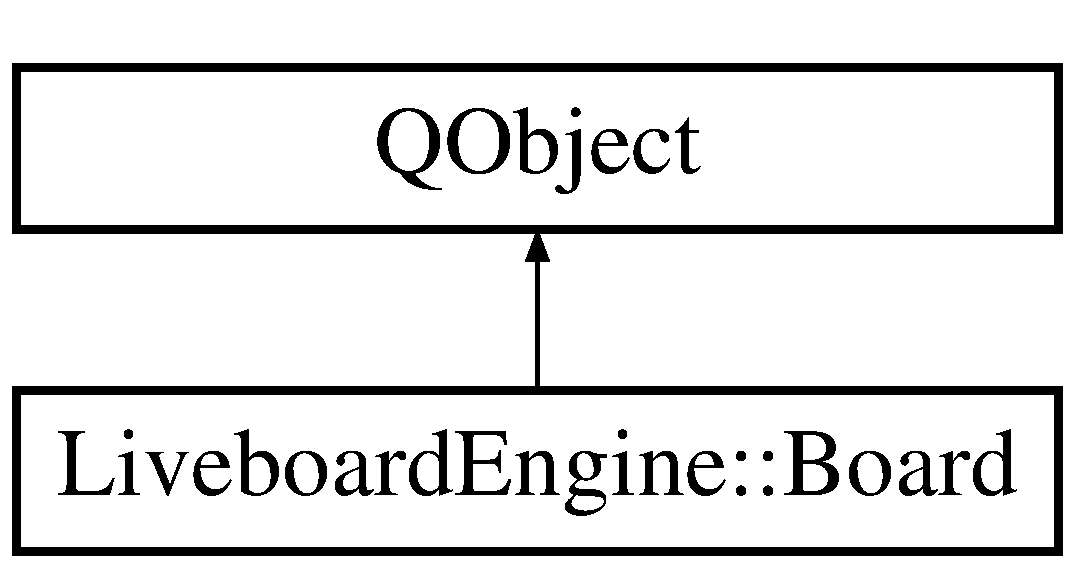
\includegraphics[height=2.000000cm]{classLiveboardEngine_1_1Board}
\end{center}
\end{figure}
\subsection*{Public Types}
\begin{DoxyCompactItemize}
\item 
\mbox{\Hypertarget{classLiveboardEngine_1_1Board_a40e707889f6ba898bc5628dbf251fcdf}\label{classLiveboardEngine_1_1Board_a40e707889f6ba898bc5628dbf251fcdf}} 
enum {\bfseries Mode} \{ {\bfseries A\+R\+R\+I\+V\+A\+LS}, 
{\bfseries D\+E\+P\+A\+R\+T\+U\+R\+ES}
 \}
\end{DoxyCompactItemize}
\subsection*{Signals}
\begin{DoxyCompactItemize}
\item 
\mbox{\Hypertarget{classLiveboardEngine_1_1Board_a3730ecf6b49c607984cccac4a0ec8db0}\label{classLiveboardEngine_1_1Board_a3730ecf6b49c607984cccac4a0ec8db0}} 
void {\bfseries entries\+Changed} ()
\item 
\mbox{\Hypertarget{classLiveboardEngine_1_1Board_acfc6c7e16ad579dbc55e1a1a5189f016}\label{classLiveboardEngine_1_1Board_acfc6c7e16ad579dbc55e1a1a5189f016}} 
void {\bfseries station\+Changed} ()
\item 
\mbox{\Hypertarget{classLiveboardEngine_1_1Board_a531c4cb3e17fda5a4f8144b9f75608cd}\label{classLiveboardEngine_1_1Board_a531c4cb3e17fda5a4f8144b9f75608cd}} 
void {\bfseries from\+Changed} ()
\item 
\mbox{\Hypertarget{classLiveboardEngine_1_1Board_af1e8c4bf8a6ccc7f6a19b7c4f34d7ac1}\label{classLiveboardEngine_1_1Board_af1e8c4bf8a6ccc7f6a19b7c4f34d7ac1}} 
void {\bfseries until\+Changed} ()
\item 
\mbox{\Hypertarget{classLiveboardEngine_1_1Board_addf2a9878bea4937fd1a5021437eef3d}\label{classLiveboardEngine_1_1Board_addf2a9878bea4937fd1a5021437eef3d}} 
void {\bfseries mode\+Changed} ()
\end{DoxyCompactItemize}
\subsection*{Public Member Functions}
\begin{DoxyCompactItemize}
\item 
\mbox{\Hypertarget{classLiveboardEngine_1_1Board_a70370a5f86db87e9edb9ca23de58b38b}\label{classLiveboardEngine_1_1Board_a70370a5f86db87e9edb9ca23de58b38b}} 
{\bfseries Board} (Q\+Object $\ast$parent=nullptr)
\item 
\mbox{\Hypertarget{classLiveboardEngine_1_1Board_ae1f97006ef5590a3b4c6b27f48c83c1f}\label{classLiveboardEngine_1_1Board_ae1f97006ef5590a3b4c6b27f48c83c1f}} 
{\bfseries Board} (const Q\+List$<$ \mbox{\hyperlink{classVehicleEngine_1_1Vehicle}{Vehicle\+Engine\+::\+Vehicle}} $\ast$$>$ \&entries, \mbox{\hyperlink{classStationEngine_1_1Station}{Station\+Engine\+::\+Station}} $\ast$station, const Q\+Date\+Time \&from, const Q\+Date\+Time \&until, Q\+Object $\ast$parent=nullptr)
\item 
\mbox{\Hypertarget{classLiveboardEngine_1_1Board_abda2c74a02ab090986147ef538337645}\label{classLiveboardEngine_1_1Board_abda2c74a02ab090986147ef538337645}} 
void {\bfseries add\+Entry} (\mbox{\hyperlink{classVehicleEngine_1_1Vehicle}{Vehicle\+Engine\+::\+Vehicle}} $\ast$entry)
\item 
\mbox{\Hypertarget{classLiveboardEngine_1_1Board_a73fd7f8c8ff5f69da644ed20798059d1}\label{classLiveboardEngine_1_1Board_a73fd7f8c8ff5f69da644ed20798059d1}} 
Q\+List$<$ \mbox{\hyperlink{classVehicleEngine_1_1Vehicle}{Vehicle\+Engine\+::\+Vehicle}} $\ast$ $>$ {\bfseries entries} () const
\item 
\mbox{\Hypertarget{classLiveboardEngine_1_1Board_a35d5d7a4b24e0f051d1e53ce7bb94761}\label{classLiveboardEngine_1_1Board_a35d5d7a4b24e0f051d1e53ce7bb94761}} 
void {\bfseries set\+Entries} (const Q\+List$<$ \mbox{\hyperlink{classVehicleEngine_1_1Vehicle}{Vehicle\+Engine\+::\+Vehicle}} $\ast$$>$ \&entries)
\item 
\mbox{\Hypertarget{classLiveboardEngine_1_1Board_a1f477aa1637a52fdaff701cb4897c3f0}\label{classLiveboardEngine_1_1Board_a1f477aa1637a52fdaff701cb4897c3f0}} 
\mbox{\hyperlink{classStationEngine_1_1Station}{Station\+Engine\+::\+Station}} $\ast$ {\bfseries station} () const
\item 
\mbox{\Hypertarget{classLiveboardEngine_1_1Board_aa68cbd2bec552af0227238b592e7c048}\label{classLiveboardEngine_1_1Board_aa68cbd2bec552af0227238b592e7c048}} 
void {\bfseries set\+Station} (\mbox{\hyperlink{classStationEngine_1_1Station}{Station\+Engine\+::\+Station}} $\ast$station)
\item 
\mbox{\Hypertarget{classLiveboardEngine_1_1Board_a23f1e2c32589a58dfe13a939cd6b1eae}\label{classLiveboardEngine_1_1Board_a23f1e2c32589a58dfe13a939cd6b1eae}} 
Q\+Date\+Time {\bfseries from} () const
\item 
\mbox{\Hypertarget{classLiveboardEngine_1_1Board_a54367a8ed3f970e4b5a11667e07196e2}\label{classLiveboardEngine_1_1Board_a54367a8ed3f970e4b5a11667e07196e2}} 
void {\bfseries set\+From} (const Q\+Date\+Time \&from)
\item 
\mbox{\Hypertarget{classLiveboardEngine_1_1Board_a37b083f54af4b4950342ef3fb526d4da}\label{classLiveboardEngine_1_1Board_a37b083f54af4b4950342ef3fb526d4da}} 
Q\+Date\+Time {\bfseries until} () const
\item 
\mbox{\Hypertarget{classLiveboardEngine_1_1Board_a9618784ccc0e9a6df84f35f0bcc83785}\label{classLiveboardEngine_1_1Board_a9618784ccc0e9a6df84f35f0bcc83785}} 
void {\bfseries set\+Until} (const Q\+Date\+Time \&until)
\item 
\mbox{\Hypertarget{classLiveboardEngine_1_1Board_ac176d818e8f72ed241852b7487dfc49b}\label{classLiveboardEngine_1_1Board_ac176d818e8f72ed241852b7487dfc49b}} 
Liveboard\+Engine\+::\+Board\+::\+Mode {\bfseries mode} () const
\item 
\mbox{\Hypertarget{classLiveboardEngine_1_1Board_aff2aefd7d785e700e122f21563072e66}\label{classLiveboardEngine_1_1Board_aff2aefd7d785e700e122f21563072e66}} 
void {\bfseries set\+Mode} (const Liveboard\+Engine\+::\+Board\+::\+Mode \&mode)
\end{DoxyCompactItemize}
\subsection*{Private Attributes}
\begin{DoxyCompactItemize}
\item 
\mbox{\Hypertarget{classLiveboardEngine_1_1Board_a0f83c2dd26626f955927bffa92c5f5f5}\label{classLiveboardEngine_1_1Board_a0f83c2dd26626f955927bffa92c5f5f5}} 
Q\+List$<$ \mbox{\hyperlink{classVehicleEngine_1_1Vehicle}{Vehicle\+Engine\+::\+Vehicle}} $\ast$ $>$ {\bfseries m\+\_\+entries}
\item 
\mbox{\Hypertarget{classLiveboardEngine_1_1Board_a1ff93cd110c4d8afd23745500b384e38}\label{classLiveboardEngine_1_1Board_a1ff93cd110c4d8afd23745500b384e38}} 
\mbox{\hyperlink{classStationEngine_1_1Station}{Station\+Engine\+::\+Station}} $\ast$ {\bfseries m\+\_\+station}
\item 
\mbox{\Hypertarget{classLiveboardEngine_1_1Board_aab66196ab496ad45bd07e5652eb24eb2}\label{classLiveboardEngine_1_1Board_aab66196ab496ad45bd07e5652eb24eb2}} 
Q\+Date\+Time {\bfseries m\+\_\+from}
\item 
\mbox{\Hypertarget{classLiveboardEngine_1_1Board_ad68f8d703d1a747b5cb0d8c12abc685d}\label{classLiveboardEngine_1_1Board_ad68f8d703d1a747b5cb0d8c12abc685d}} 
Q\+Date\+Time {\bfseries m\+\_\+until}
\item 
\mbox{\Hypertarget{classLiveboardEngine_1_1Board_a1dde2228349f7f97ddd6191b1df07712}\label{classLiveboardEngine_1_1Board_a1dde2228349f7f97ddd6191b1df07712}} 
Liveboard\+Engine\+::\+Board\+::\+Mode {\bfseries m\+\_\+mode}
\end{DoxyCompactItemize}


The documentation for this class was generated from the following files\+:\begin{DoxyCompactItemize}
\item 
src/include/engines/liveboard/liveboardboard.\+h\item 
src/engines/liveboard/\mbox{\hyperlink{liveboardboard_8cpp}{liveboardboard.\+cpp}}\end{DoxyCompactItemize}

\hypertarget{classLiveboardEngine_1_1Factory}{}\section{Liveboard\+Engine\+:\+:Factory Class Reference}
\label{classLiveboardEngine_1_1Factory}\index{Liveboard\+Engine\+::\+Factory@{Liveboard\+Engine\+::\+Factory}}
Inheritance diagram for Liveboard\+Engine\+:\+:Factory\+:\begin{figure}[H]
\begin{center}
\leavevmode
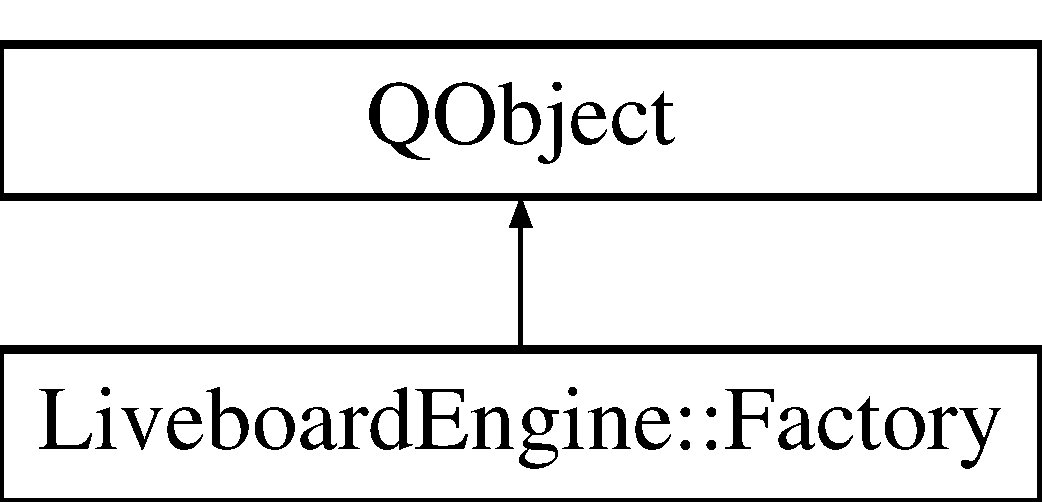
\includegraphics[height=2.000000cm]{classLiveboardEngine_1_1Factory}
\end{center}
\end{figure}
\subsection*{Signals}
\begin{DoxyCompactItemize}
\item 
\mbox{\Hypertarget{classLiveboardEngine_1_1Factory_adfd318c2ca3b7852ae6fb8f2ec6c531d}\label{classLiveboardEngine_1_1Factory_adfd318c2ca3b7852ae6fb8f2ec6c531d}} 
void {\bfseries liveboard\+Ready} (\mbox{\hyperlink{classLiveboardEngine_1_1Board}{Liveboard\+Engine\+::\+Board}} $\ast$liveboard)
\item 
\mbox{\Hypertarget{classLiveboardEngine_1_1Factory_aecd8f5df55d1a7604f9f93f8420df015}\label{classLiveboardEngine_1_1Factory_aecd8f5df55d1a7604f9f93f8420df015}} 
void {\bfseries from\+Changed} ()
\item 
\mbox{\Hypertarget{classLiveboardEngine_1_1Factory_a41c86f68cdef04156116d8519c2fa040}\label{classLiveboardEngine_1_1Factory_a41c86f68cdef04156116d8519c2fa040}} 
void {\bfseries until\+Changed} ()
\item 
\mbox{\Hypertarget{classLiveboardEngine_1_1Factory_ab849fa14c77ca43c0aa62f3e44775d69}\label{classLiveboardEngine_1_1Factory_ab849fa14c77ca43c0aa62f3e44775d69}} 
void {\bfseries station\+U\+R\+I\+Changed} ()
\item 
\mbox{\Hypertarget{classLiveboardEngine_1_1Factory_a7b7b0b3dff6670b4603174c79f0e22fa}\label{classLiveboardEngine_1_1Factory_a7b7b0b3dff6670b4603174c79f0e22fa}} 
void {\bfseries mode\+Changed} ()
\item 
\mbox{\Hypertarget{classLiveboardEngine_1_1Factory_ac688f2fe85e61735f8c8caea1ffacc2b}\label{classLiveboardEngine_1_1Factory_ac688f2fe85e61735f8c8caea1ffacc2b}} 
void {\bfseries page\+Received} (const Q\+Url \&uri)
\item 
\mbox{\Hypertarget{classLiveboardEngine_1_1Factory_a7b90ae3a8251afc0a76316d180fe8d40}\label{classLiveboardEngine_1_1Factory_a7b90ae3a8251afc0a76316d180fe8d40}} 
void {\bfseries page\+Requested} (const Q\+Url \&uri)
\end{DoxyCompactItemize}
\subsection*{Public Member Functions}
\begin{DoxyCompactItemize}
\item 
\mbox{\Hypertarget{classLiveboardEngine_1_1Factory_a806d17edc5fb9687cc56d40e47607c56}\label{classLiveboardEngine_1_1Factory_a806d17edc5fb9687cc56d40e47607c56}} 
void {\bfseries get\+Liveboard\+By\+Station\+U\+RI} (const Q\+Url \&uri, const Liveboard\+Engine\+::\+Board\+::\+Mode \&mode=Liveboard\+Engine\+::\+Board\+::\+Mode\+::\+D\+E\+P\+A\+R\+T\+U\+R\+ES)
\item 
\mbox{\Hypertarget{classLiveboardEngine_1_1Factory_addcb51b3e2aea11e927ea4336d1d8136}\label{classLiveboardEngine_1_1Factory_addcb51b3e2aea11e927ea4336d1d8136}} 
void {\bfseries get\+Liveboard\+By\+Station\+U\+RI} (const Q\+Url \&uri, const Q\+Date\+Time \&from, const Q\+Date\+Time \&until, const Liveboard\+Engine\+::\+Board\+::\+Mode \&mode=Liveboard\+Engine\+::\+Board\+::\+Mode\+::\+D\+E\+P\+A\+R\+T\+U\+R\+ES)
\item 
\mbox{\Hypertarget{classLiveboardEngine_1_1Factory_a8baf19d418f12486528dd107b0e40bff}\label{classLiveboardEngine_1_1Factory_a8baf19d418f12486528dd107b0e40bff}} 
Q\+Date\+Time {\bfseries from} () const
\item 
\mbox{\Hypertarget{classLiveboardEngine_1_1Factory_a42f78670fbec877ac3209fb30d6e5d37}\label{classLiveboardEngine_1_1Factory_a42f78670fbec877ac3209fb30d6e5d37}} 
Q\+Date\+Time {\bfseries until} () const
\item 
\mbox{\Hypertarget{classLiveboardEngine_1_1Factory_aa6b3c6593412c0cdb805a0f64b779035}\label{classLiveboardEngine_1_1Factory_aa6b3c6593412c0cdb805a0f64b779035}} 
Q\+Url {\bfseries station\+U\+RI} () const
\item 
\mbox{\Hypertarget{classLiveboardEngine_1_1Factory_a066656be247d7c91ddd55bd2e0dba9e1}\label{classLiveboardEngine_1_1Factory_a066656be247d7c91ddd55bd2e0dba9e1}} 
Liveboard\+Engine\+::\+Board\+::\+Mode {\bfseries mode} () const
\item 
\mbox{\Hypertarget{classLiveboardEngine_1_1Factory_a65f9e5079dce07a63e68ced303438797}\label{classLiveboardEngine_1_1Factory_a65f9e5079dce07a63e68ced303438797}} 
\mbox{\hyperlink{classLiveboardEngine_1_1Board}{Liveboard\+Engine\+::\+Board}} $\ast$ {\bfseries liveboard} () const
\end{DoxyCompactItemize}
\subsection*{Static Public Member Functions}
\begin{DoxyCompactItemize}
\item 
\mbox{\Hypertarget{classLiveboardEngine_1_1Factory_af5820597b574ffe1a3b20fb2c080aa00}\label{classLiveboardEngine_1_1Factory_af5820597b574ffe1a3b20fb2c080aa00}} 
static \mbox{\hyperlink{classLiveboardEngine_1_1Factory}{Liveboard\+Engine\+::\+Factory}} $\ast$ {\bfseries get\+Instance} ()
\end{DoxyCompactItemize}
\subsection*{Private Slots}
\begin{DoxyCompactItemize}
\item 
\mbox{\Hypertarget{classLiveboardEngine_1_1Factory_a0201463446beff21ab5fceb64f56ad50}\label{classLiveboardEngine_1_1Factory_a0201463446beff21ab5fceb64f56ad50}} 
void {\bfseries page\+Received} (\mbox{\hyperlink{classFragments_1_1Page}{Fragments\+::\+Page}} $\ast$page)
\end{DoxyCompactItemize}
\subsection*{Private Member Functions}
\begin{DoxyCompactItemize}
\item 
\mbox{\Hypertarget{classLiveboardEngine_1_1Factory_ab90c1ee0ead367bbd75ed69823fe486f}\label{classLiveboardEngine_1_1Factory_ab90c1ee0ead367bbd75ed69823fe486f}} 
\mbox{\hyperlink{classFragments_1_1Factory}{Fragments\+::\+Factory}} $\ast$ {\bfseries fragments\+Factory} () const
\item 
\mbox{\Hypertarget{classLiveboardEngine_1_1Factory_a7bfcb03543a49a277347512d81c6db34}\label{classLiveboardEngine_1_1Factory_a7bfcb03543a49a277347512d81c6db34}} 
\mbox{\hyperlink{classStationEngine_1_1Factory}{Station\+Engine\+::\+Factory}} $\ast$ {\bfseries station\+Factory} () const
\item 
\mbox{\Hypertarget{classLiveboardEngine_1_1Factory_ac4e57f9038fdeb983321fd68dc833e6a}\label{classLiveboardEngine_1_1Factory_ac4e57f9038fdeb983321fd68dc833e6a}} 
void {\bfseries set\+Station\+Factory} (\mbox{\hyperlink{classStationEngine_1_1Factory}{Station\+Engine\+::\+Factory}} $\ast$station\+Factory)
\item 
\mbox{\Hypertarget{classLiveboardEngine_1_1Factory_aa806f015edf7a559e3e536d408706006}\label{classLiveboardEngine_1_1Factory_aa806f015edf7a559e3e536d408706006}} 
void {\bfseries parse\+Page} (\mbox{\hyperlink{classFragments_1_1Page}{Fragments\+::\+Page}} $\ast$page, const bool \&finished)
\item 
\mbox{\Hypertarget{classLiveboardEngine_1_1Factory_a279c353aaa01c123521e732b83ffa33d}\label{classLiveboardEngine_1_1Factory_a279c353aaa01c123521e732b83ffa33d}} 
void {\bfseries set\+Fragments\+Factory} (\mbox{\hyperlink{classFragments_1_1Factory}{Fragments\+::\+Factory}} $\ast$fragments\+Factory)
\item 
\mbox{\Hypertarget{classLiveboardEngine_1_1Factory_a7d34790a70c3648bb131a50a6d3e6d89}\label{classLiveboardEngine_1_1Factory_a7d34790a70c3648bb131a50a6d3e6d89}} 
void {\bfseries set\+Mode} (const Liveboard\+Engine\+::\+Board\+::\+Mode \&mode)
\item 
\mbox{\Hypertarget{classLiveboardEngine_1_1Factory_a0f1b6032456353dde732bf7e57801aa8}\label{classLiveboardEngine_1_1Factory_a0f1b6032456353dde732bf7e57801aa8}} 
void {\bfseries set\+Station\+U\+RI} (const Q\+Url \&station\+U\+RI)
\item 
\mbox{\Hypertarget{classLiveboardEngine_1_1Factory_adfb070f58b28a55be0f44a81acc44863}\label{classLiveboardEngine_1_1Factory_adfb070f58b28a55be0f44a81acc44863}} 
void {\bfseries set\+Until} (const Q\+Date\+Time \&until)
\item 
\mbox{\Hypertarget{classLiveboardEngine_1_1Factory_a1cb666c3dd962fd95d7a82faa3c7977b}\label{classLiveboardEngine_1_1Factory_a1cb666c3dd962fd95d7a82faa3c7977b}} 
void {\bfseries set\+From} (const Q\+Date\+Time \&from)
\item 
\mbox{\Hypertarget{classLiveboardEngine_1_1Factory_a2b320b1d62e58d4640adfc28ff3bb1b2}\label{classLiveboardEngine_1_1Factory_a2b320b1d62e58d4640adfc28ff3bb1b2}} 
void {\bfseries set\+Liveboard} (\mbox{\hyperlink{classLiveboardEngine_1_1Board}{Liveboard\+Engine\+::\+Board}} $\ast$liveboard)
\item 
\mbox{\Hypertarget{classLiveboardEngine_1_1Factory_a48031c644406c9f4c5216afccbcd31ae}\label{classLiveboardEngine_1_1Factory_a48031c644406c9f4c5216afccbcd31ae}} 
{\bfseries Factory} (Q\+Object $\ast$parent=nullptr)
\end{DoxyCompactItemize}
\subsection*{Private Attributes}
\begin{DoxyCompactItemize}
\item 
\mbox{\Hypertarget{classLiveboardEngine_1_1Factory_a0bbd9cca03d43800f5d4621d1685fbb1}\label{classLiveboardEngine_1_1Factory_a0bbd9cca03d43800f5d4621d1685fbb1}} 
Q\+Mutex {\bfseries liveboard\+Access\+Mutex}
\item 
\mbox{\Hypertarget{classLiveboardEngine_1_1Factory_ab0c26a56e06ae85f336d57c3cf65c840}\label{classLiveboardEngine_1_1Factory_ab0c26a56e06ae85f336d57c3cf65c840}} 
\mbox{\hyperlink{classLiveboardEngine_1_1Board}{Liveboard\+Engine\+::\+Board}} $\ast$ {\bfseries m\+\_\+liveboard}
\item 
\mbox{\Hypertarget{classLiveboardEngine_1_1Factory_a431320530f78df90fbfab06fb9a19fe1}\label{classLiveboardEngine_1_1Factory_a431320530f78df90fbfab06fb9a19fe1}} 
Q\+Date\+Time {\bfseries m\+\_\+from}
\item 
\mbox{\Hypertarget{classLiveboardEngine_1_1Factory_a784255d4b92213d1a6d3defe68a0e576}\label{classLiveboardEngine_1_1Factory_a784255d4b92213d1a6d3defe68a0e576}} 
Q\+Date\+Time {\bfseries m\+\_\+until}
\item 
\mbox{\Hypertarget{classLiveboardEngine_1_1Factory_a65ba0fc99dc4a73eefcce0cc65db2f8e}\label{classLiveboardEngine_1_1Factory_a65ba0fc99dc4a73eefcce0cc65db2f8e}} 
Q\+Url {\bfseries m\+\_\+station\+U\+RI}
\item 
\mbox{\Hypertarget{classLiveboardEngine_1_1Factory_a76adf5433e6da144ff3b7dd6749ff0c4}\label{classLiveboardEngine_1_1Factory_a76adf5433e6da144ff3b7dd6749ff0c4}} 
Liveboard\+Engine\+::\+Board\+::\+Mode {\bfseries m\+\_\+mode}
\item 
\mbox{\Hypertarget{classLiveboardEngine_1_1Factory_afeb512b65d2c46c3e7b037725a6b7fa4}\label{classLiveboardEngine_1_1Factory_afeb512b65d2c46c3e7b037725a6b7fa4}} 
\mbox{\hyperlink{classFragments_1_1Factory}{Fragments\+::\+Factory}} $\ast$ {\bfseries m\+\_\+fragments\+Factory}
\item 
\mbox{\Hypertarget{classLiveboardEngine_1_1Factory_afddd77a02b368c8147180d7b88a22135}\label{classLiveboardEngine_1_1Factory_afddd77a02b368c8147180d7b88a22135}} 
\mbox{\hyperlink{classStationEngine_1_1Factory}{Station\+Engine\+::\+Factory}} $\ast$ {\bfseries m\+\_\+station\+Factory}
\end{DoxyCompactItemize}
\subsection*{Static Private Attributes}
\begin{DoxyCompactItemize}
\item 
\mbox{\Hypertarget{classLiveboardEngine_1_1Factory_ad5a5c61d1196a8f7433b7e2b8e41ca64}\label{classLiveboardEngine_1_1Factory_ad5a5c61d1196a8f7433b7e2b8e41ca64}} 
static \mbox{\hyperlink{classLiveboardEngine_1_1Factory}{Liveboard\+Engine\+::\+Factory}} $\ast$ {\bfseries m\+\_\+instance} = nullptr
\end{DoxyCompactItemize}


The documentation for this class was generated from the following files\+:\begin{DoxyCompactItemize}
\item 
src/include/engines/liveboard/liveboardfactory.\+h\item 
src/engines/liveboard/\mbox{\hyperlink{liveboardfactory_8cpp}{liveboardfactory.\+cpp}}\end{DoxyCompactItemize}

\hypertarget{classFragments_1_1Factory}{}\section{Fragments\+:\+:Factory Class Reference}
\label{classFragments_1_1Factory}\index{Fragments\+::\+Factory@{Fragments\+::\+Factory}}


{\ttfamily \#include $<$fragmentsfactory.\+h$>$}

Inheritance diagram for Fragments\+:\+:Factory\+:\begin{figure}[H]
\begin{center}
\leavevmode
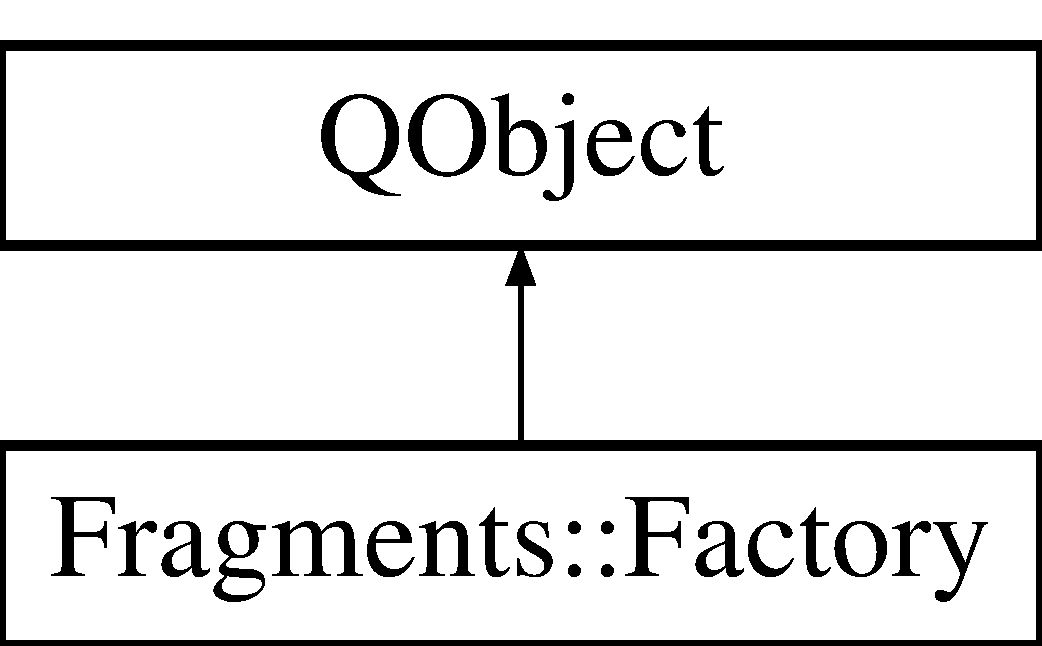
\includegraphics[height=2.000000cm]{classFragments_1_1Factory}
\end{center}
\end{figure}
\subsection*{Signals}
\begin{DoxyCompactItemize}
\item 
void \mbox{\hyperlink{classFragments_1_1Factory_a9559b78a9960c0d4981bf752b47d710a}{page\+Ready}} (\mbox{\hyperlink{classFragments_1_1Page}{Fragments\+::\+Page}} $\ast$page)
\item 
void \mbox{\hyperlink{classFragments_1_1Factory_ac65f072a6cc48bb340e89a61c30688d6}{get\+Resource}} (const Q\+Url \&uri)
\item 
void \mbox{\hyperlink{classFragments_1_1Factory_ab8bdc67290ccbc5444d551fbebc68b17}{error}} (const Q\+String \&message)
\end{DoxyCompactItemize}
\subsection*{Public Member Functions}
\begin{DoxyCompactItemize}
\item 
void \mbox{\hyperlink{classFragments_1_1Factory_a37e59ac23a1a4889a5ef9348f1dfd0bc}{get\+Page}} (const Q\+Url \&uri)
\item 
void \mbox{\hyperlink{classFragments_1_1Factory_a3c9b46f2158e91190305b25616a4bc34}{get\+Page}} (const Q\+Date\+Time \&departure\+Time)
\end{DoxyCompactItemize}
\subsection*{Static Public Member Functions}
\begin{DoxyCompactItemize}
\item 
static \mbox{\hyperlink{classFragments_1_1Factory}{Fragments\+::\+Factory}} $\ast$ \mbox{\hyperlink{classFragments_1_1Factory_a32614388e70b2737a28c045ebbe58e55}{get\+Instance}} (Q\+Object $\ast$parent=nullptr)
\end{DoxyCompactItemize}
\subsection*{Private Slots}
\begin{DoxyCompactItemize}
\item 
void \mbox{\hyperlink{classFragments_1_1Factory_a0ee4ef4c4521a4bce9fe901236a14c84}{process\+H\+T\+T\+P\+Reply}} (Q\+Network\+Reply $\ast$reply)
\end{DoxyCompactItemize}
\subsection*{Private Member Functions}
\begin{DoxyCompactItemize}
\item 
void \mbox{\hyperlink{classFragments_1_1Factory_a9a5923caf97c4e8dba24e23539328deb}{get\+Page\+By\+U\+R\+I\+From\+Network\+Manager}} (const Q\+Url \&uri)
\item 
\mbox{\hyperlink{classFragments_1_1Fragment}{Fragments\+::\+Fragment}} $\ast$ \mbox{\hyperlink{classFragments_1_1Factory_a8f78a634fbeec2b7edb731d778947e97}{generate\+Fragment\+From\+J\+S\+ON}} (const Q\+Json\+Object \&connection)
\item 
bool \mbox{\hyperlink{classFragments_1_1Factory_a62a60fd81fec95b794a8b27188b51824}{validate\+Data}} (const Q\+Json\+Object \&data, const Q\+String\+List \&properties)
\item 
\mbox{\hyperlink{classFragments_1_1Factory_a04aefdf80a3318302fbb839b9322a12e}{Factory}} (Q\+Object $\ast$parent)
\item 
\mbox{\hyperlink{classNetwork_1_1Manager}{Network\+::\+Manager}} $\ast$ \mbox{\hyperlink{classFragments_1_1Factory_ae9f54ac342a7fd5010689d80ef343424}{http}} () const
\item 
void \mbox{\hyperlink{classFragments_1_1Factory_ae5738a3e881b1791dda120e34be3cea9}{set\+Http}} (\mbox{\hyperlink{classNetwork_1_1Manager}{Network\+::\+Manager}} $\ast$\mbox{\hyperlink{classFragments_1_1Factory_ae9f54ac342a7fd5010689d80ef343424}{http}})
\end{DoxyCompactItemize}
\subsection*{Private Attributes}
\begin{DoxyCompactItemize}
\item 
\mbox{\hyperlink{classNetwork_1_1Manager}{Network\+::\+Manager}} $\ast$ \mbox{\hyperlink{classFragments_1_1Factory_aa98b2097fdc55511bdf4fc3bda37e98e}{m\+\_\+http}}
\end{DoxyCompactItemize}
\subsection*{Static Private Attributes}
\begin{DoxyCompactItemize}
\item 
static \mbox{\hyperlink{classFragments_1_1Factory}{Fragments\+::\+Factory}} $\ast$ \mbox{\hyperlink{classFragments_1_1Factory_a7e07aaa093813ab0e1cb50e92ac1386e}{m\+\_\+instance}} = nullptr
\end{DoxyCompactItemize}


\subsection{Constructor \& Destructor Documentation}
\mbox{\Hypertarget{classFragments_1_1Factory_a04aefdf80a3318302fbb839b9322a12e}\label{classFragments_1_1Factory_a04aefdf80a3318302fbb839b9322a12e}} 
\index{Fragments\+::\+Factory@{Fragments\+::\+Factory}!Factory@{Factory}}
\index{Factory@{Factory}!Fragments\+::\+Factory@{Fragments\+::\+Factory}}
\subsubsection{\texorpdfstring{Factory()}{Factory()}}
{\footnotesize\ttfamily Fragments\+::\+Factory\+::\+Factory (\begin{DoxyParamCaption}\item[{Q\+Object $\ast$}]{parent }\end{DoxyParamCaption})\hspace{0.3cm}{\ttfamily [explicit]}, {\ttfamily [private]}}



\subsection{Member Function Documentation}
\mbox{\Hypertarget{classFragments_1_1Factory_ab8bdc67290ccbc5444d551fbebc68b17}\label{classFragments_1_1Factory_ab8bdc67290ccbc5444d551fbebc68b17}} 
\index{Fragments\+::\+Factory@{Fragments\+::\+Factory}!error@{error}}
\index{error@{error}!Fragments\+::\+Factory@{Fragments\+::\+Factory}}
\subsubsection{\texorpdfstring{error}{error}}
{\footnotesize\ttfamily void Fragments\+::\+Factory\+::error (\begin{DoxyParamCaption}\item[{const Q\+String \&}]{message }\end{DoxyParamCaption})\hspace{0.3cm}{\ttfamily [signal]}}

\mbox{\Hypertarget{classFragments_1_1Factory_a8f78a634fbeec2b7edb731d778947e97}\label{classFragments_1_1Factory_a8f78a634fbeec2b7edb731d778947e97}} 
\index{Fragments\+::\+Factory@{Fragments\+::\+Factory}!generate\+Fragment\+From\+J\+S\+ON@{generate\+Fragment\+From\+J\+S\+ON}}
\index{generate\+Fragment\+From\+J\+S\+ON@{generate\+Fragment\+From\+J\+S\+ON}!Fragments\+::\+Factory@{Fragments\+::\+Factory}}
\subsubsection{\texorpdfstring{generate\+Fragment\+From\+J\+S\+O\+N()}{generateFragmentFromJSON()}}
{\footnotesize\ttfamily \mbox{\hyperlink{classFragments_1_1Fragment}{Fragments\+::\+Fragment}} $\ast$ Fragments\+::\+Factory\+::generate\+Fragment\+From\+J\+S\+ON (\begin{DoxyParamCaption}\item[{const Q\+Json\+Object \&}]{connection }\end{DoxyParamCaption})\hspace{0.3cm}{\ttfamily [private]}}

\mbox{\Hypertarget{classFragments_1_1Factory_a32614388e70b2737a28c045ebbe58e55}\label{classFragments_1_1Factory_a32614388e70b2737a28c045ebbe58e55}} 
\index{Fragments\+::\+Factory@{Fragments\+::\+Factory}!get\+Instance@{get\+Instance}}
\index{get\+Instance@{get\+Instance}!Fragments\+::\+Factory@{Fragments\+::\+Factory}}
\subsubsection{\texorpdfstring{get\+Instance()}{getInstance()}}
{\footnotesize\ttfamily \mbox{\hyperlink{classFragments_1_1Factory}{Fragments\+::\+Factory}} $\ast$ Fragments\+::\+Factory\+::get\+Instance (\begin{DoxyParamCaption}\item[{Q\+Object $\ast$}]{parent = {\ttfamily nullptr} }\end{DoxyParamCaption})\hspace{0.3cm}{\ttfamily [static]}}

\mbox{\Hypertarget{classFragments_1_1Factory_a37e59ac23a1a4889a5ef9348f1dfd0bc}\label{classFragments_1_1Factory_a37e59ac23a1a4889a5ef9348f1dfd0bc}} 
\index{Fragments\+::\+Factory@{Fragments\+::\+Factory}!get\+Page@{get\+Page}}
\index{get\+Page@{get\+Page}!Fragments\+::\+Factory@{Fragments\+::\+Factory}}
\subsubsection{\texorpdfstring{get\+Page()}{getPage()}\hspace{0.1cm}{\footnotesize\ttfamily [1/2]}}
{\footnotesize\ttfamily void Fragments\+::\+Factory\+::get\+Page (\begin{DoxyParamCaption}\item[{const Q\+Url \&}]{uri }\end{DoxyParamCaption})}

\mbox{\Hypertarget{classFragments_1_1Factory_a3c9b46f2158e91190305b25616a4bc34}\label{classFragments_1_1Factory_a3c9b46f2158e91190305b25616a4bc34}} 
\index{Fragments\+::\+Factory@{Fragments\+::\+Factory}!get\+Page@{get\+Page}}
\index{get\+Page@{get\+Page}!Fragments\+::\+Factory@{Fragments\+::\+Factory}}
\subsubsection{\texorpdfstring{get\+Page()}{getPage()}\hspace{0.1cm}{\footnotesize\ttfamily [2/2]}}
{\footnotesize\ttfamily void Fragments\+::\+Factory\+::get\+Page (\begin{DoxyParamCaption}\item[{const Q\+Date\+Time \&}]{departure\+Time }\end{DoxyParamCaption})}

\mbox{\Hypertarget{classFragments_1_1Factory_a9a5923caf97c4e8dba24e23539328deb}\label{classFragments_1_1Factory_a9a5923caf97c4e8dba24e23539328deb}} 
\index{Fragments\+::\+Factory@{Fragments\+::\+Factory}!get\+Page\+By\+U\+R\+I\+From\+Network\+Manager@{get\+Page\+By\+U\+R\+I\+From\+Network\+Manager}}
\index{get\+Page\+By\+U\+R\+I\+From\+Network\+Manager@{get\+Page\+By\+U\+R\+I\+From\+Network\+Manager}!Fragments\+::\+Factory@{Fragments\+::\+Factory}}
\subsubsection{\texorpdfstring{get\+Page\+By\+U\+R\+I\+From\+Network\+Manager()}{getPageByURIFromNetworkManager()}}
{\footnotesize\ttfamily void Fragments\+::\+Factory\+::get\+Page\+By\+U\+R\+I\+From\+Network\+Manager (\begin{DoxyParamCaption}\item[{const Q\+Url \&}]{uri }\end{DoxyParamCaption})\hspace{0.3cm}{\ttfamily [private]}}

\mbox{\Hypertarget{classFragments_1_1Factory_ac65f072a6cc48bb340e89a61c30688d6}\label{classFragments_1_1Factory_ac65f072a6cc48bb340e89a61c30688d6}} 
\index{Fragments\+::\+Factory@{Fragments\+::\+Factory}!get\+Resource@{get\+Resource}}
\index{get\+Resource@{get\+Resource}!Fragments\+::\+Factory@{Fragments\+::\+Factory}}
\subsubsection{\texorpdfstring{get\+Resource}{getResource}}
{\footnotesize\ttfamily void Fragments\+::\+Factory\+::get\+Resource (\begin{DoxyParamCaption}\item[{const Q\+Url \&}]{uri }\end{DoxyParamCaption})\hspace{0.3cm}{\ttfamily [signal]}}

\mbox{\Hypertarget{classFragments_1_1Factory_ae9f54ac342a7fd5010689d80ef343424}\label{classFragments_1_1Factory_ae9f54ac342a7fd5010689d80ef343424}} 
\index{Fragments\+::\+Factory@{Fragments\+::\+Factory}!http@{http}}
\index{http@{http}!Fragments\+::\+Factory@{Fragments\+::\+Factory}}
\subsubsection{\texorpdfstring{http()}{http()}}
{\footnotesize\ttfamily \mbox{\hyperlink{classNetwork_1_1Manager}{Network\+::\+Manager}} $\ast$ Fragments\+::\+Factory\+::http (\begin{DoxyParamCaption}{ }\end{DoxyParamCaption}) const\hspace{0.3cm}{\ttfamily [private]}}

\mbox{\Hypertarget{classFragments_1_1Factory_a9559b78a9960c0d4981bf752b47d710a}\label{classFragments_1_1Factory_a9559b78a9960c0d4981bf752b47d710a}} 
\index{Fragments\+::\+Factory@{Fragments\+::\+Factory}!page\+Ready@{page\+Ready}}
\index{page\+Ready@{page\+Ready}!Fragments\+::\+Factory@{Fragments\+::\+Factory}}
\subsubsection{\texorpdfstring{page\+Ready}{pageReady}}
{\footnotesize\ttfamily void Fragments\+::\+Factory\+::page\+Ready (\begin{DoxyParamCaption}\item[{\mbox{\hyperlink{classFragments_1_1Page}{Fragments\+::\+Page}} $\ast$}]{page }\end{DoxyParamCaption})\hspace{0.3cm}{\ttfamily [signal]}}

\mbox{\Hypertarget{classFragments_1_1Factory_a0ee4ef4c4521a4bce9fe901236a14c84}\label{classFragments_1_1Factory_a0ee4ef4c4521a4bce9fe901236a14c84}} 
\index{Fragments\+::\+Factory@{Fragments\+::\+Factory}!process\+H\+T\+T\+P\+Reply@{process\+H\+T\+T\+P\+Reply}}
\index{process\+H\+T\+T\+P\+Reply@{process\+H\+T\+T\+P\+Reply}!Fragments\+::\+Factory@{Fragments\+::\+Factory}}
\subsubsection{\texorpdfstring{process\+H\+T\+T\+P\+Reply}{processHTTPReply}}
{\footnotesize\ttfamily void Fragments\+::\+Factory\+::process\+H\+T\+T\+P\+Reply (\begin{DoxyParamCaption}\item[{Q\+Network\+Reply $\ast$}]{reply }\end{DoxyParamCaption})\hspace{0.3cm}{\ttfamily [private]}, {\ttfamily [slot]}}

\mbox{\Hypertarget{classFragments_1_1Factory_ae5738a3e881b1791dda120e34be3cea9}\label{classFragments_1_1Factory_ae5738a3e881b1791dda120e34be3cea9}} 
\index{Fragments\+::\+Factory@{Fragments\+::\+Factory}!set\+Http@{set\+Http}}
\index{set\+Http@{set\+Http}!Fragments\+::\+Factory@{Fragments\+::\+Factory}}
\subsubsection{\texorpdfstring{set\+Http()}{setHttp()}}
{\footnotesize\ttfamily void Fragments\+::\+Factory\+::set\+Http (\begin{DoxyParamCaption}\item[{\mbox{\hyperlink{classNetwork_1_1Manager}{Network\+::\+Manager}} $\ast$}]{http }\end{DoxyParamCaption})\hspace{0.3cm}{\ttfamily [private]}}

\mbox{\Hypertarget{classFragments_1_1Factory_a62a60fd81fec95b794a8b27188b51824}\label{classFragments_1_1Factory_a62a60fd81fec95b794a8b27188b51824}} 
\index{Fragments\+::\+Factory@{Fragments\+::\+Factory}!validate\+Data@{validate\+Data}}
\index{validate\+Data@{validate\+Data}!Fragments\+::\+Factory@{Fragments\+::\+Factory}}
\subsubsection{\texorpdfstring{validate\+Data()}{validateData()}}
{\footnotesize\ttfamily bool Fragments\+::\+Factory\+::validate\+Data (\begin{DoxyParamCaption}\item[{const Q\+Json\+Object \&}]{data,  }\item[{const Q\+String\+List \&}]{properties }\end{DoxyParamCaption})\hspace{0.3cm}{\ttfamily [private]}}



\subsection{Member Data Documentation}
\mbox{\Hypertarget{classFragments_1_1Factory_aa98b2097fdc55511bdf4fc3bda37e98e}\label{classFragments_1_1Factory_aa98b2097fdc55511bdf4fc3bda37e98e}} 
\index{Fragments\+::\+Factory@{Fragments\+::\+Factory}!m\+\_\+http@{m\+\_\+http}}
\index{m\+\_\+http@{m\+\_\+http}!Fragments\+::\+Factory@{Fragments\+::\+Factory}}
\subsubsection{\texorpdfstring{m\+\_\+http}{m\_http}}
{\footnotesize\ttfamily \mbox{\hyperlink{classNetwork_1_1Manager}{Network\+::\+Manager}}$\ast$ Fragments\+::\+Factory\+::m\+\_\+http\hspace{0.3cm}{\ttfamily [private]}}

\mbox{\Hypertarget{classFragments_1_1Factory_a7e07aaa093813ab0e1cb50e92ac1386e}\label{classFragments_1_1Factory_a7e07aaa093813ab0e1cb50e92ac1386e}} 
\index{Fragments\+::\+Factory@{Fragments\+::\+Factory}!m\+\_\+instance@{m\+\_\+instance}}
\index{m\+\_\+instance@{m\+\_\+instance}!Fragments\+::\+Factory@{Fragments\+::\+Factory}}
\subsubsection{\texorpdfstring{m\+\_\+instance}{m\_instance}}
{\footnotesize\ttfamily \mbox{\hyperlink{classFragments_1_1Factory}{Fragments\+::\+Factory}} $\ast$ Fragments\+::\+Factory\+::m\+\_\+instance = nullptr\hspace{0.3cm}{\ttfamily [static]}, {\ttfamily [private]}}



The documentation for this class was generated from the following files\+:\begin{DoxyCompactItemize}
\item 
src/linkedconnections/fragments/\mbox{\hyperlink{fragmentsfactory_8h}{fragmentsfactory.\+h}}\item 
src/linkedconnections/fragments/\mbox{\hyperlink{fragmentsfactory_8cpp}{fragmentsfactory.\+cpp}}\end{DoxyCompactItemize}

\hypertarget{classStationEngine_1_1Factory}{}\section{Station\+Engine\+:\+:Factory Class Reference}
\label{classStationEngine_1_1Factory}\index{Station\+Engine\+::\+Factory@{Station\+Engine\+::\+Factory}}
Inheritance diagram for Station\+Engine\+:\+:Factory\+:\begin{figure}[H]
\begin{center}
\leavevmode
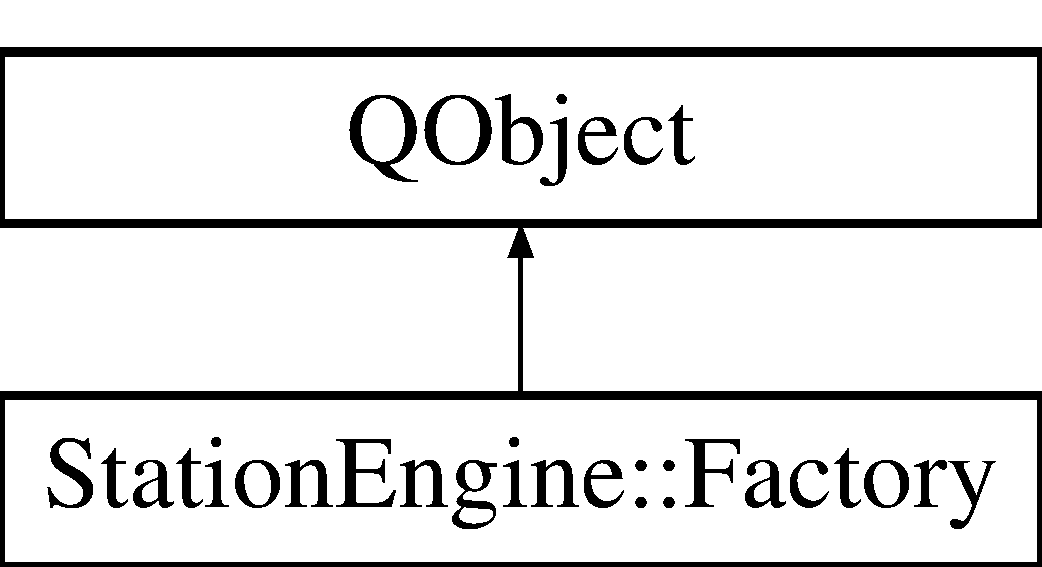
\includegraphics[height=2.000000cm]{classStationEngine_1_1Factory}
\end{center}
\end{figure}
\subsection*{Public Member Functions}
\begin{DoxyCompactItemize}
\item 
\mbox{\Hypertarget{classStationEngine_1_1Factory_ad7b0c3ee3716d2a99643c0c7b0b9a9c0}\label{classStationEngine_1_1Factory_ad7b0c3ee3716d2a99643c0c7b0b9a9c0}} 
\mbox{\hyperlink{classStationEngine_1_1Station}{Station}} $\ast$ {\bfseries get\+Station\+By\+U\+RI} (const Q\+Url \&uri)
\end{DoxyCompactItemize}
\subsection*{Static Public Member Functions}
\begin{DoxyCompactItemize}
\item 
\mbox{\Hypertarget{classStationEngine_1_1Factory_a2bca26c84868868d0a58e8313a70a80c}\label{classStationEngine_1_1Factory_a2bca26c84868868d0a58e8313a70a80c}} 
static \mbox{\hyperlink{classStationEngine_1_1Factory}{Factory}} $\ast$ {\bfseries get\+Instance} ()
\end{DoxyCompactItemize}
\subsection*{Private Member Functions}
\begin{DoxyCompactItemize}
\item 
\mbox{\Hypertarget{classStationEngine_1_1Factory_ae97fddbe0a8ef42024bd1b9a295b5a1a}\label{classStationEngine_1_1Factory_ae97fddbe0a8ef42024bd1b9a295b5a1a}} 
bool {\bfseries init\+Database} ()
\item 
\mbox{\Hypertarget{classStationEngine_1_1Factory_ab8c16d5f36fa5ab4d55f4648e5b9de85}\label{classStationEngine_1_1Factory_ab8c16d5f36fa5ab4d55f4648e5b9de85}} 
Q\+Future$<$ bool $>$ {\bfseries insert\+Station\+With\+Facilities\+Into\+Database} (const Q\+String\+List \&station, const Q\+String\+List \&facilities)
\item 
\mbox{\Hypertarget{classStationEngine_1_1Factory_a390ba2b14c1473025470b077202d095f}\label{classStationEngine_1_1Factory_a390ba2b14c1473025470b077202d095f}} 
Q\+Future$<$ bool $>$ {\bfseries insert\+Station\+Without\+Facilities\+Into\+Database} (const Q\+String\+List \&station)
\item 
\mbox{\Hypertarget{classStationEngine_1_1Factory_abbd0d01d21431b969955e3515848a615}\label{classStationEngine_1_1Factory_abbd0d01d21431b969955e3515848a615}} 
Q\+Future$<$ bool $>$ {\bfseries insert\+Platform\+Into\+Database} (const Q\+String\+List \&stop)
\item 
\mbox{\Hypertarget{classStationEngine_1_1Factory_a3f9a807b6019f8c85b11445f4de8d8ba}\label{classStationEngine_1_1Factory_a3f9a807b6019f8c85b11445f4de8d8ba}} 
\mbox{\hyperlink{classStationEngine_1_1Station}{Station\+Engine\+::\+Station}} $\ast$ {\bfseries fetch\+Station\+From\+Cache} (const Q\+Url \&uri) const
\item 
\mbox{\Hypertarget{classStationEngine_1_1Factory_a4b9c7838d8e88b0ee429d26b3936e464}\label{classStationEngine_1_1Factory_a4b9c7838d8e88b0ee429d26b3936e464}} 
void {\bfseries add\+Station\+To\+Cache} (\mbox{\hyperlink{classStationEngine_1_1Station}{Station\+Engine\+::\+Station}} $\ast$station)
\item 
\mbox{\Hypertarget{classStationEngine_1_1Factory_a35a0cfd90547e76c5d5612073fd7a331}\label{classStationEngine_1_1Factory_a35a0cfd90547e76c5d5612073fd7a331}} 
Q\+Map$<$ Q\+Url, Q\+String $>$ {\bfseries get\+Platforms\+By\+Station\+U\+RI} (const Q\+Url \&uri)
\item 
\mbox{\Hypertarget{classStationEngine_1_1Factory_ab871018160a944731e87db4c772e377e}\label{classStationEngine_1_1Factory_ab871018160a944731e87db4c772e377e}} 
\mbox{\hyperlink{classDatabase_1_1Manager}{Database\+::\+Manager}} $\ast$ {\bfseries db} () const
\item 
\mbox{\Hypertarget{classStationEngine_1_1Factory_a12aaa48831c5baed1f1d275c4a812546}\label{classStationEngine_1_1Factory_a12aaa48831c5baed1f1d275c4a812546}} 
void {\bfseries set\+Db} (\mbox{\hyperlink{classDatabase_1_1Manager}{Database\+::\+Manager}} $\ast$db)
\item 
\mbox{\Hypertarget{classStationEngine_1_1Factory_a5171ed076e2b451562a5a8483f875e2b}\label{classStationEngine_1_1Factory_a5171ed076e2b451562a5a8483f875e2b}} 
{\bfseries Factory} (Q\+Object $\ast$parent=nullptr)
\end{DoxyCompactItemize}
\subsection*{Private Attributes}
\begin{DoxyCompactItemize}
\item 
\mbox{\Hypertarget{classStationEngine_1_1Factory_a5e37413b221a5ef8aeec50adc239029a}\label{classStationEngine_1_1Factory_a5e37413b221a5ef8aeec50adc239029a}} 
\mbox{\hyperlink{classDatabase_1_1Manager}{Database\+::\+Manager}} $\ast$ {\bfseries m\+\_\+db}
\item 
\mbox{\Hypertarget{classStationEngine_1_1Factory_ae267ebb3f7372f61420ff91475204a21}\label{classStationEngine_1_1Factory_ae267ebb3f7372f61420ff91475204a21}} 
Q\+Map$<$ Q\+Url, \mbox{\hyperlink{classStationEngine_1_1Station}{Station\+Engine\+::\+Station}} $\ast$ $>$ {\bfseries m\+\_\+cache}
\end{DoxyCompactItemize}
\subsection*{Static Private Attributes}
\begin{DoxyCompactItemize}
\item 
\mbox{\Hypertarget{classStationEngine_1_1Factory_ab38580988730892e9d2c1553b491609a}\label{classStationEngine_1_1Factory_ab38580988730892e9d2c1553b491609a}} 
static \mbox{\hyperlink{classStationEngine_1_1Factory}{Station\+Engine\+::\+Factory}} $\ast$ {\bfseries m\+\_\+instance} = nullptr
\end{DoxyCompactItemize}


The documentation for this class was generated from the following files\+:\begin{DoxyCompactItemize}
\item 
src/include/engines/station/stationfactory.\+h\item 
src/engines/station/\mbox{\hyperlink{stationfactory_8cpp}{stationfactory.\+cpp}}\end{DoxyCompactItemize}

\hypertarget{classVehicleEngine_1_1Factory}{}\section{Vehicle\+Engine\+:\+:Factory Class Reference}
\label{classVehicleEngine_1_1Factory}\index{Vehicle\+Engine\+::\+Factory@{Vehicle\+Engine\+::\+Factory}}
Inheritance diagram for Vehicle\+Engine\+:\+:Factory\+:\begin{figure}[H]
\begin{center}
\leavevmode
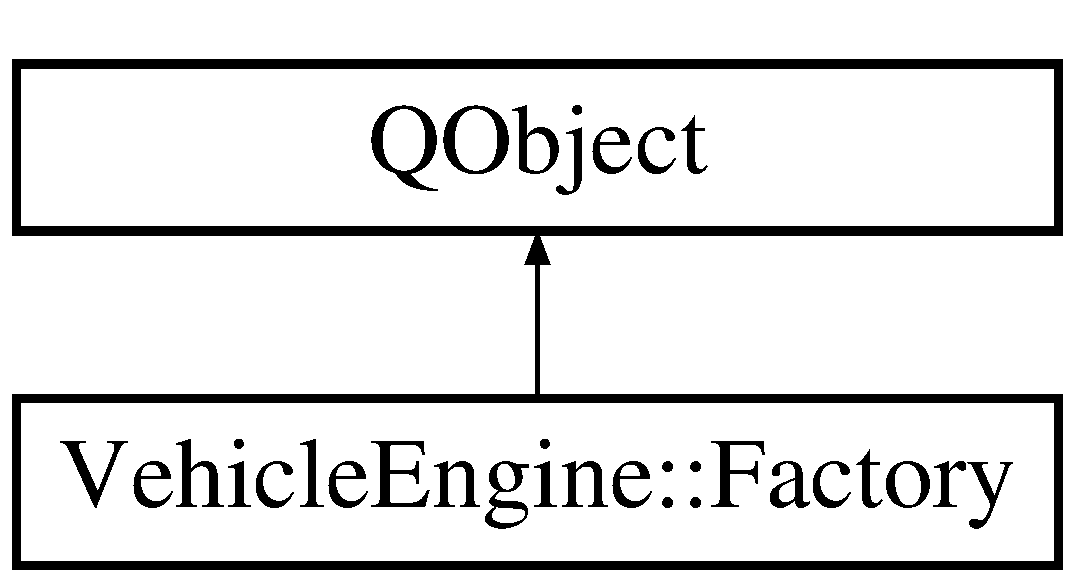
\includegraphics[height=2.000000cm]{classVehicleEngine_1_1Factory}
\end{center}
\end{figure}
\subsection*{Signals}
\begin{DoxyCompactItemize}
\item 
\mbox{\Hypertarget{classVehicleEngine_1_1Factory_af23bdc01d77eb6c9feb7f79f00511c22}\label{classVehicleEngine_1_1Factory_af23bdc01d77eb6c9feb7f79f00511c22}} 
void {\bfseries vehicle\+Ready} (\mbox{\hyperlink{classVehicleEngine_1_1Vehicle}{Vehicle\+Engine\+::\+Vehicle}} $\ast$vehicle)
\item 
\mbox{\Hypertarget{classVehicleEngine_1_1Factory_a72f608e6196d6e0824302c914baf5247}\label{classVehicleEngine_1_1Factory_a72f608e6196d6e0824302c914baf5247}} 
void {\bfseries get\+Resource} (const Q\+Url \&uri)
\item 
\mbox{\Hypertarget{classVehicleEngine_1_1Factory_a6f3a429ae4109615d43d75fb9dc0767d}\label{classVehicleEngine_1_1Factory_a6f3a429ae4109615d43d75fb9dc0767d}} 
void {\bfseries error} (const Q\+String \&message)
\end{DoxyCompactItemize}
\subsection*{Public Member Functions}
\begin{DoxyCompactItemize}
\item 
\mbox{\Hypertarget{classVehicleEngine_1_1Factory_a217155cea1486b498ac22f9f1dbaf5d6}\label{classVehicleEngine_1_1Factory_a217155cea1486b498ac22f9f1dbaf5d6}} 
void {\bfseries get\+Vehicle\+By\+U\+RI} (const Q\+Url \&uri, const Q\+Locale\+::\+Language \&language)
\item 
\mbox{\Hypertarget{classVehicleEngine_1_1Factory_a209085165273b23198942c1ff0253fa9}\label{classVehicleEngine_1_1Factory_a209085165273b23198942c1ff0253fa9}} 
Q\+Locale\+::\+Language {\bfseries language} () const
\item 
\mbox{\Hypertarget{classVehicleEngine_1_1Factory_ad1c125ca1398b70e3be6f8997050823b}\label{classVehicleEngine_1_1Factory_ad1c125ca1398b70e3be6f8997050823b}} 
void {\bfseries set\+Language} (const Q\+Locale\+::\+Language \&language)
\end{DoxyCompactItemize}
\subsection*{Static Public Member Functions}
\begin{DoxyCompactItemize}
\item 
\mbox{\Hypertarget{classVehicleEngine_1_1Factory_aac29410d8cbfa22f0f47f52dd2d8ab3d}\label{classVehicleEngine_1_1Factory_aac29410d8cbfa22f0f47f52dd2d8ab3d}} 
static \mbox{\hyperlink{classVehicleEngine_1_1Factory}{Vehicle\+Engine\+::\+Factory}} $\ast$ {\bfseries get\+Instance} ()
\end{DoxyCompactItemize}
\subsection*{Private Slots}
\begin{DoxyCompactItemize}
\item 
\mbox{\Hypertarget{classVehicleEngine_1_1Factory_acd692b52ab3ccb817ea4a54d427d9226}\label{classVehicleEngine_1_1Factory_acd692b52ab3ccb817ea4a54d427d9226}} 
void {\bfseries process\+H\+T\+T\+P\+Reply} (Q\+Network\+Reply $\ast$reply)
\end{DoxyCompactItemize}
\subsection*{Private Member Functions}
\begin{DoxyCompactItemize}
\item 
\mbox{\Hypertarget{classVehicleEngine_1_1Factory_a2e2e49cee65a409309492354de57b496}\label{classVehicleEngine_1_1Factory_a2e2e49cee65a409309492354de57b496}} 
bool {\bfseries validate\+Data} (const Q\+Json\+Object \&data, const Q\+String\+List \&properties)
\item 
\mbox{\Hypertarget{classVehicleEngine_1_1Factory_ad9754d9052aad8c82d34ab41988b5d88}\label{classVehicleEngine_1_1Factory_ad9754d9052aad8c82d34ab41988b5d88}} 
\mbox{\hyperlink{classNetwork_1_1Manager}{Network\+::\+Manager}} $\ast$ {\bfseries http} () const
\item 
\mbox{\Hypertarget{classVehicleEngine_1_1Factory_ac0be65c70dc1288e6897fcdb4d2f4a30}\label{classVehicleEngine_1_1Factory_ac0be65c70dc1288e6897fcdb4d2f4a30}} 
void {\bfseries set\+Http} (\mbox{\hyperlink{classNetwork_1_1Manager}{Network\+::\+Manager}} $\ast$http)
\item 
\mbox{\Hypertarget{classVehicleEngine_1_1Factory_a8b2dd9ea47df9ed7a62664b6542236fc}\label{classVehicleEngine_1_1Factory_a8b2dd9ea47df9ed7a62664b6542236fc}} 
\mbox{\hyperlink{classStationEngine_1_1Factory}{Station\+Engine\+::\+Factory}} $\ast$ {\bfseries station\+Factory} () const
\item 
\mbox{\Hypertarget{classVehicleEngine_1_1Factory_a2fad7421921f211b993c2271b0e8548a}\label{classVehicleEngine_1_1Factory_a2fad7421921f211b993c2271b0e8548a}} 
void {\bfseries set\+Station\+Factory} (\mbox{\hyperlink{classStationEngine_1_1Factory}{Station\+Engine\+::\+Factory}} $\ast$station\+Factory)
\item 
\mbox{\Hypertarget{classVehicleEngine_1_1Factory_a897b4f8f42d0c57a1aabc36d850d16e5}\label{classVehicleEngine_1_1Factory_a897b4f8f42d0c57a1aabc36d850d16e5}} 
\mbox{\hyperlink{classVehicleEngine_1_1Stop}{Vehicle\+Engine\+::\+Stop}} $\ast$ {\bfseries generate\+Stop\+From\+J\+S\+ON} (const Q\+Json\+Object \&stop)
\item 
\mbox{\Hypertarget{classVehicleEngine_1_1Factory_abc5d1a7173c2f6be23c68a44d575127e}\label{classVehicleEngine_1_1Factory_abc5d1a7173c2f6be23c68a44d575127e}} 
Vehicle\+Engine\+::\+Stop\+::\+Occupancy\+Level {\bfseries generate\+Occupancy\+Level\+From\+J\+S\+ON} (const Q\+Json\+Object \&occupancy) const
\item 
\mbox{\Hypertarget{classVehicleEngine_1_1Factory_ac013f1c3e3089e2c8081897c326098c5}\label{classVehicleEngine_1_1Factory_ac013f1c3e3089e2c8081897c326098c5}} 
{\bfseries Factory} (Q\+Object $\ast$parent=nullptr)
\end{DoxyCompactItemize}
\subsection*{Private Attributes}
\begin{DoxyCompactItemize}
\item 
\mbox{\Hypertarget{classVehicleEngine_1_1Factory_a7db189c0fa5d68eda7f90ffd0d4ed48f}\label{classVehicleEngine_1_1Factory_a7db189c0fa5d68eda7f90ffd0d4ed48f}} 
\mbox{\hyperlink{classNetwork_1_1Manager}{Network\+::\+Manager}} $\ast$ {\bfseries m\+\_\+http}
\item 
\mbox{\Hypertarget{classVehicleEngine_1_1Factory_a2f8e99563781a2901e4814d262453871}\label{classVehicleEngine_1_1Factory_a2f8e99563781a2901e4814d262453871}} 
\mbox{\hyperlink{classStationEngine_1_1Factory}{Station\+Engine\+::\+Factory}} $\ast$ {\bfseries m\+\_\+station\+Factory}
\item 
\mbox{\Hypertarget{classVehicleEngine_1_1Factory_a00ca9db84ea9227d62d201479a9342ff}\label{classVehicleEngine_1_1Factory_a00ca9db84ea9227d62d201479a9342ff}} 
Q\+Locale\+::\+Language {\bfseries m\+\_\+language}
\end{DoxyCompactItemize}
\subsection*{Static Private Attributes}
\begin{DoxyCompactItemize}
\item 
\mbox{\Hypertarget{classVehicleEngine_1_1Factory_a000d443fa44673ab1931a2fa5c1a786c}\label{classVehicleEngine_1_1Factory_a000d443fa44673ab1931a2fa5c1a786c}} 
static \mbox{\hyperlink{classVehicleEngine_1_1Factory}{Vehicle\+Engine\+::\+Factory}} $\ast$ {\bfseries m\+\_\+instance} = nullptr
\end{DoxyCompactItemize}


The documentation for this class was generated from the following files\+:\begin{DoxyCompactItemize}
\item 
src/include/engines/vehicle/\mbox{\hyperlink{vehiclefactory_8h}{vehiclefactory.\+h}}\item 
src/engines/vehicle/\mbox{\hyperlink{vehiclefactory_8cpp}{vehiclefactory.\+cpp}}\end{DoxyCompactItemize}

\hypertarget{classFragments_1_1Fragment}{}\section{Fragments\+:\+:Fragment Class Reference}
\label{classFragments_1_1Fragment}\index{Fragments\+::\+Fragment@{Fragments\+::\+Fragment}}


{\ttfamily \#include $<$fragmentsfragment.\+h$>$}

Inheritance diagram for Fragments\+:\+:Fragment\+:\begin{figure}[H]
\begin{center}
\leavevmode
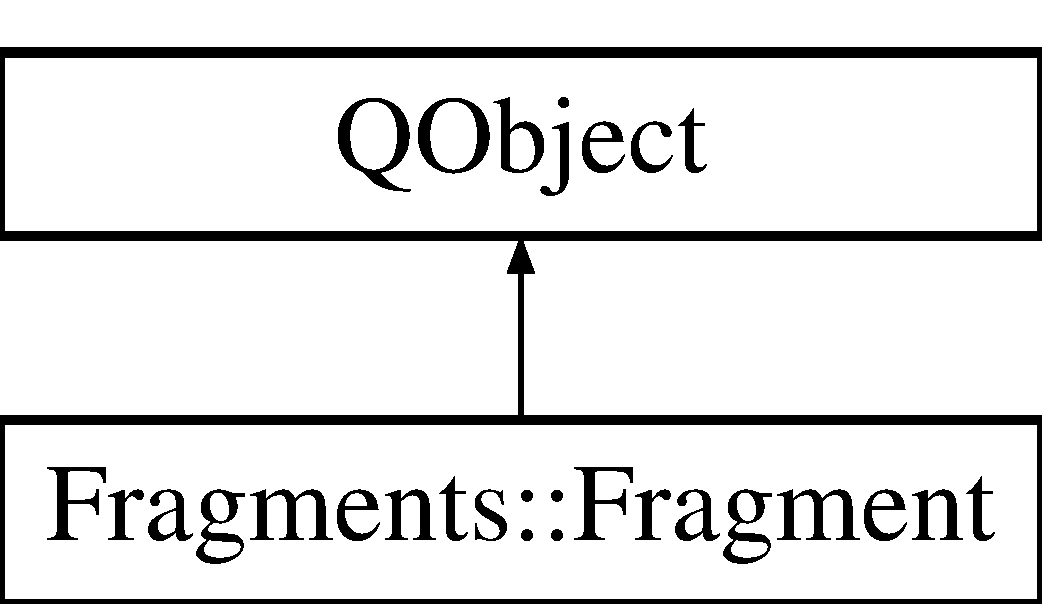
\includegraphics[height=2.000000cm]{classFragments_1_1Fragment}
\end{center}
\end{figure}
\subsection*{Signals}
\begin{DoxyCompactItemize}
\item 
void \mbox{\hyperlink{classFragments_1_1Fragment_ad1d14027cf24dea3982576f160ed61e4}{uri\+Changed}} ()
\item 
void \mbox{\hyperlink{classFragments_1_1Fragment_add02014358cc604a4d5473ff317b9048}{departure\+Station\+U\+R\+I\+Changed}} ()
\item 
void \mbox{\hyperlink{classFragments_1_1Fragment_ab3afd2b0cd0d1fe7a0dc15cd7c358195}{arrival\+Station\+U\+R\+I\+Changed}} ()
\item 
void \mbox{\hyperlink{classFragments_1_1Fragment_a3b4eaf02e54dcf202c5b740c6e3946e6}{departure\+Time\+Changed}} ()
\item 
void \mbox{\hyperlink{classFragments_1_1Fragment_a25530427fe0bc865f7595221a8284ef2}{arrival\+Time\+Changed}} ()
\item 
void \mbox{\hyperlink{classFragments_1_1Fragment_a2f4407d54a869e2a45b514525c582016}{departure\+Delay\+Changed}} ()
\item 
void \mbox{\hyperlink{classFragments_1_1Fragment_a586fd07ea637247637da6971555ed92b}{arrival\+Delay\+Changed}} ()
\item 
void \mbox{\hyperlink{classFragments_1_1Fragment_a80a2dcba09a29a4d375b8900bb6b6be0}{trip\+U\+R\+I\+Changed}} ()
\item 
void \mbox{\hyperlink{classFragments_1_1Fragment_ab220e9fef71bf161e14769afc61f0499}{route\+U\+R\+I\+Changed}} ()
\item 
void \mbox{\hyperlink{classFragments_1_1Fragment_a5956fb561df3842d6d292b46fc16bec2}{direction\+Changed}} ()
\end{DoxyCompactItemize}
\subsection*{Public Member Functions}
\begin{DoxyCompactItemize}
\item 
\mbox{\hyperlink{classFragments_1_1Fragment_a08e16b988d340a5e836c377a13e1c41d}{Fragment}} (Q\+Object $\ast$parent=nullptr)
\item 
\mbox{\hyperlink{classFragments_1_1Fragment_a26ec3793c4162b77e92498a77ae5b7dc}{Fragment}} (const Q\+Url \&\mbox{\hyperlink{classFragments_1_1Fragment_a8123bbbb75221107730898627b99ffec}{uri}}, const Q\+Url \&\mbox{\hyperlink{classFragments_1_1Fragment_aaca4de063cdd1df3f130ade1a0df8dfa}{departure\+Station\+U\+RI}}, const Q\+Url \&\mbox{\hyperlink{classFragments_1_1Fragment_a74d2fae0d687f2389121fb720f8f6505}{arrival\+Station\+U\+RI}}, const Q\+Date\+Time \&\mbox{\hyperlink{classFragments_1_1Fragment_adfcf2bb9a548f41f4ca88ad117c655a3}{departure\+Time}}, const Q\+Date\+Time \&\mbox{\hyperlink{classFragments_1_1Fragment_aa7e96d4d8b9e36c19d3f6134ff3072e9}{arrival\+Time}}, const qint16 \&\mbox{\hyperlink{classFragments_1_1Fragment_a8c8363f22d1aca339a66d342f9e5f0c8}{departure\+Delay}}, const qint16 \&\mbox{\hyperlink{classFragments_1_1Fragment_aec60f571141b0c7aacbc172e83a4a2d3}{arrival\+Delay}}, const Q\+Url \&\mbox{\hyperlink{classFragments_1_1Fragment_aa3b1beb97e501bfa8ecb2127c2729803}{trip\+U\+RI}}, const Q\+Url \&\mbox{\hyperlink{classFragments_1_1Fragment_a58ca3c71db8995b1a60b1eee17d65911}{route\+U\+RI}}, const Q\+String \&\mbox{\hyperlink{classFragments_1_1Fragment_a1c0ff28939d612a28589fdc1f47d0fd5}{direction}}, Q\+Object $\ast$parent=nullptr)
\item 
Q\+Url \mbox{\hyperlink{classFragments_1_1Fragment_a8123bbbb75221107730898627b99ffec}{uri}} () const
\item 
void \mbox{\hyperlink{classFragments_1_1Fragment_ab4ad3107834caa289cfbed904f052fc0}{set\+U\+RI}} (const Q\+Url \&\mbox{\hyperlink{classFragments_1_1Fragment_a8123bbbb75221107730898627b99ffec}{uri}})
\item 
Q\+Url \mbox{\hyperlink{classFragments_1_1Fragment_aaca4de063cdd1df3f130ade1a0df8dfa}{departure\+Station\+U\+RI}} () const
\item 
void \mbox{\hyperlink{classFragments_1_1Fragment_a8c9ffce21e97be8e50e2ca1654da507f}{set\+Departure\+Station\+U\+RI}} (const Q\+Url \&\mbox{\hyperlink{classFragments_1_1Fragment_aaca4de063cdd1df3f130ade1a0df8dfa}{departure\+Station\+U\+RI}})
\item 
Q\+Url \mbox{\hyperlink{classFragments_1_1Fragment_a74d2fae0d687f2389121fb720f8f6505}{arrival\+Station\+U\+RI}} () const
\item 
void \mbox{\hyperlink{classFragments_1_1Fragment_af18c29375ad402d4ec02133fb5534a8e}{set\+Arrival\+Station\+U\+RI}} (const Q\+Url \&\mbox{\hyperlink{classFragments_1_1Fragment_a74d2fae0d687f2389121fb720f8f6505}{arrival\+Station\+U\+RI}})
\item 
Q\+Date\+Time \mbox{\hyperlink{classFragments_1_1Fragment_adfcf2bb9a548f41f4ca88ad117c655a3}{departure\+Time}} () const
\item 
void \mbox{\hyperlink{classFragments_1_1Fragment_a595b2c52c5cbaab0a97ceda63028d91d}{set\+Departure\+Time}} (const Q\+Date\+Time \&\mbox{\hyperlink{classFragments_1_1Fragment_adfcf2bb9a548f41f4ca88ad117c655a3}{departure\+Time}})
\item 
Q\+Date\+Time \mbox{\hyperlink{classFragments_1_1Fragment_aa7e96d4d8b9e36c19d3f6134ff3072e9}{arrival\+Time}} () const
\item 
void \mbox{\hyperlink{classFragments_1_1Fragment_a5b7ed13c7d4417f3b4f3d87aebd68a90}{set\+Arrival\+Time}} (const Q\+Date\+Time \&\mbox{\hyperlink{classFragments_1_1Fragment_aa7e96d4d8b9e36c19d3f6134ff3072e9}{arrival\+Time}})
\item 
qint16 \mbox{\hyperlink{classFragments_1_1Fragment_a8c8363f22d1aca339a66d342f9e5f0c8}{departure\+Delay}} () const
\item 
void \mbox{\hyperlink{classFragments_1_1Fragment_a3293b86baeee32223a5019594fb1ae82}{set\+Departure\+Delay}} (const qint16 \&\mbox{\hyperlink{classFragments_1_1Fragment_a8c8363f22d1aca339a66d342f9e5f0c8}{departure\+Delay}})
\item 
qint16 \mbox{\hyperlink{classFragments_1_1Fragment_aec60f571141b0c7aacbc172e83a4a2d3}{arrival\+Delay}} () const
\item 
void \mbox{\hyperlink{classFragments_1_1Fragment_ae5df59623d6835ec0224d58f9f3903db}{set\+Arrival\+Delay}} (const qint16 \&\mbox{\hyperlink{classFragments_1_1Fragment_aec60f571141b0c7aacbc172e83a4a2d3}{arrival\+Delay}})
\item 
Q\+Date\+Time \mbox{\hyperlink{classFragments_1_1Fragment_a23f4a6f0401e2d2e6aa2f53621beefa0}{departure\+Delayed\+Time}} () const
\item 
Q\+Date\+Time \mbox{\hyperlink{classFragments_1_1Fragment_a9948ab3690d2c290eda2adc89415e2b2}{arrival\+Delayed\+Time}} () const
\item 
Q\+Url \mbox{\hyperlink{classFragments_1_1Fragment_aa3b1beb97e501bfa8ecb2127c2729803}{trip\+U\+RI}} () const
\item 
void \mbox{\hyperlink{classFragments_1_1Fragment_a47c214a918ce0fe7469b309cbecf01a1}{set\+Trip\+U\+RI}} (const Q\+Url \&\mbox{\hyperlink{classFragments_1_1Fragment_aa3b1beb97e501bfa8ecb2127c2729803}{trip\+U\+RI}})
\item 
Q\+Url \mbox{\hyperlink{classFragments_1_1Fragment_a58ca3c71db8995b1a60b1eee17d65911}{route\+U\+RI}} () const
\item 
void \mbox{\hyperlink{classFragments_1_1Fragment_a26880f6f3800e4609685f1316b6db257}{set\+Route\+U\+RI}} (const Q\+Url \&\mbox{\hyperlink{classFragments_1_1Fragment_a58ca3c71db8995b1a60b1eee17d65911}{route\+U\+RI}})
\item 
Q\+String \mbox{\hyperlink{classFragments_1_1Fragment_a1c0ff28939d612a28589fdc1f47d0fd5}{direction}} () const
\item 
void \mbox{\hyperlink{classFragments_1_1Fragment_a0de734da455ac32aad779520d9cc7a10}{set\+Direction}} (const Q\+String \&\mbox{\hyperlink{classFragments_1_1Fragment_a1c0ff28939d612a28589fdc1f47d0fd5}{direction}})
\end{DoxyCompactItemize}
\subsection*{Private Attributes}
\begin{DoxyCompactItemize}
\item 
Q\+Url \mbox{\hyperlink{classFragments_1_1Fragment_a5e60c2e6902a55c1e2a3bb7a97d390f5}{m\+\_\+uri}}
\item 
Q\+Url \mbox{\hyperlink{classFragments_1_1Fragment_ad283a69630de2d45564976d8f4f20494}{m\+\_\+departure\+Station\+U\+RI}}
\item 
Q\+Url \mbox{\hyperlink{classFragments_1_1Fragment_ae7965d7528238e79ad22fd5f07666913}{m\+\_\+arrival\+Station\+U\+RI}}
\item 
Q\+Date\+Time \mbox{\hyperlink{classFragments_1_1Fragment_a0e8fdc91c05e8770524e5069e63a1c8d}{m\+\_\+departure\+Time}}
\item 
Q\+Date\+Time \mbox{\hyperlink{classFragments_1_1Fragment_ae9a5e9389dbe68090f9b14a73cf6ec32}{m\+\_\+arrival\+Time}}
\item 
qint16 \mbox{\hyperlink{classFragments_1_1Fragment_a4191e1af11c31f3b6e87ec860e2a51e1}{m\+\_\+departure\+Delay}}
\item 
qint16 \mbox{\hyperlink{classFragments_1_1Fragment_ab73eb5dd910919a3b74da379489ab51e}{m\+\_\+arrival\+Delay}}
\item 
Q\+Url \mbox{\hyperlink{classFragments_1_1Fragment_abd0750b77264363fe0069764fd7aeb3c}{m\+\_\+trip\+U\+RI}}
\item 
Q\+Url \mbox{\hyperlink{classFragments_1_1Fragment_a7540fc6c97499e59d7bc582bfc142dbb}{m\+\_\+route\+U\+RI}}
\item 
Q\+String \mbox{\hyperlink{classFragments_1_1Fragment_acc9b5abffc1a65636063e42943a9e529}{m\+\_\+direction}}
\end{DoxyCompactItemize}


\subsection{Constructor \& Destructor Documentation}
\mbox{\Hypertarget{classFragments_1_1Fragment_a08e16b988d340a5e836c377a13e1c41d}\label{classFragments_1_1Fragment_a08e16b988d340a5e836c377a13e1c41d}} 
\index{Fragments\+::\+Fragment@{Fragments\+::\+Fragment}!Fragment@{Fragment}}
\index{Fragment@{Fragment}!Fragments\+::\+Fragment@{Fragments\+::\+Fragment}}
\subsubsection{\texorpdfstring{Fragment()}{Fragment()}\hspace{0.1cm}{\footnotesize\ttfamily [1/2]}}
{\footnotesize\ttfamily Fragments\+::\+Fragment\+::\+Fragment (\begin{DoxyParamCaption}\item[{Q\+Object $\ast$}]{parent = {\ttfamily nullptr} }\end{DoxyParamCaption})\hspace{0.3cm}{\ttfamily [explicit]}}

\mbox{\Hypertarget{classFragments_1_1Fragment_a26ec3793c4162b77e92498a77ae5b7dc}\label{classFragments_1_1Fragment_a26ec3793c4162b77e92498a77ae5b7dc}} 
\index{Fragments\+::\+Fragment@{Fragments\+::\+Fragment}!Fragment@{Fragment}}
\index{Fragment@{Fragment}!Fragments\+::\+Fragment@{Fragments\+::\+Fragment}}
\subsubsection{\texorpdfstring{Fragment()}{Fragment()}\hspace{0.1cm}{\footnotesize\ttfamily [2/2]}}
{\footnotesize\ttfamily Fragments\+::\+Fragment\+::\+Fragment (\begin{DoxyParamCaption}\item[{const Q\+Url \&}]{uri,  }\item[{const Q\+Url \&}]{departure\+Station\+U\+RI,  }\item[{const Q\+Url \&}]{arrival\+Station\+U\+RI,  }\item[{const Q\+Date\+Time \&}]{departure\+Time,  }\item[{const Q\+Date\+Time \&}]{arrival\+Time,  }\item[{const qint16 \&}]{departure\+Delay,  }\item[{const qint16 \&}]{arrival\+Delay,  }\item[{const Q\+Url \&}]{trip\+U\+RI,  }\item[{const Q\+Url \&}]{route\+U\+RI,  }\item[{const Q\+String \&}]{direction,  }\item[{Q\+Object $\ast$}]{parent = {\ttfamily nullptr} }\end{DoxyParamCaption})\hspace{0.3cm}{\ttfamily [explicit]}}



\subsection{Member Function Documentation}
\mbox{\Hypertarget{classFragments_1_1Fragment_aec60f571141b0c7aacbc172e83a4a2d3}\label{classFragments_1_1Fragment_aec60f571141b0c7aacbc172e83a4a2d3}} 
\index{Fragments\+::\+Fragment@{Fragments\+::\+Fragment}!arrival\+Delay@{arrival\+Delay}}
\index{arrival\+Delay@{arrival\+Delay}!Fragments\+::\+Fragment@{Fragments\+::\+Fragment}}
\subsubsection{\texorpdfstring{arrival\+Delay()}{arrivalDelay()}}
{\footnotesize\ttfamily qint16 Fragments\+::\+Fragment\+::arrival\+Delay (\begin{DoxyParamCaption}{ }\end{DoxyParamCaption}) const}

\mbox{\Hypertarget{classFragments_1_1Fragment_a586fd07ea637247637da6971555ed92b}\label{classFragments_1_1Fragment_a586fd07ea637247637da6971555ed92b}} 
\index{Fragments\+::\+Fragment@{Fragments\+::\+Fragment}!arrival\+Delay\+Changed@{arrival\+Delay\+Changed}}
\index{arrival\+Delay\+Changed@{arrival\+Delay\+Changed}!Fragments\+::\+Fragment@{Fragments\+::\+Fragment}}
\subsubsection{\texorpdfstring{arrival\+Delay\+Changed}{arrivalDelayChanged}}
{\footnotesize\ttfamily void Fragments\+::\+Fragment\+::arrival\+Delay\+Changed (\begin{DoxyParamCaption}{ }\end{DoxyParamCaption})\hspace{0.3cm}{\ttfamily [signal]}}

\mbox{\Hypertarget{classFragments_1_1Fragment_a9948ab3690d2c290eda2adc89415e2b2}\label{classFragments_1_1Fragment_a9948ab3690d2c290eda2adc89415e2b2}} 
\index{Fragments\+::\+Fragment@{Fragments\+::\+Fragment}!arrival\+Delayed\+Time@{arrival\+Delayed\+Time}}
\index{arrival\+Delayed\+Time@{arrival\+Delayed\+Time}!Fragments\+::\+Fragment@{Fragments\+::\+Fragment}}
\subsubsection{\texorpdfstring{arrival\+Delayed\+Time()}{arrivalDelayedTime()}}
{\footnotesize\ttfamily Q\+Date\+Time Fragments\+::\+Fragment\+::arrival\+Delayed\+Time (\begin{DoxyParamCaption}{ }\end{DoxyParamCaption}) const}

\mbox{\Hypertarget{classFragments_1_1Fragment_a74d2fae0d687f2389121fb720f8f6505}\label{classFragments_1_1Fragment_a74d2fae0d687f2389121fb720f8f6505}} 
\index{Fragments\+::\+Fragment@{Fragments\+::\+Fragment}!arrival\+Station\+U\+RI@{arrival\+Station\+U\+RI}}
\index{arrival\+Station\+U\+RI@{arrival\+Station\+U\+RI}!Fragments\+::\+Fragment@{Fragments\+::\+Fragment}}
\subsubsection{\texorpdfstring{arrival\+Station\+U\+R\+I()}{arrivalStationURI()}}
{\footnotesize\ttfamily Q\+Url Fragments\+::\+Fragment\+::arrival\+Station\+U\+RI (\begin{DoxyParamCaption}{ }\end{DoxyParamCaption}) const}

\mbox{\Hypertarget{classFragments_1_1Fragment_ab3afd2b0cd0d1fe7a0dc15cd7c358195}\label{classFragments_1_1Fragment_ab3afd2b0cd0d1fe7a0dc15cd7c358195}} 
\index{Fragments\+::\+Fragment@{Fragments\+::\+Fragment}!arrival\+Station\+U\+R\+I\+Changed@{arrival\+Station\+U\+R\+I\+Changed}}
\index{arrival\+Station\+U\+R\+I\+Changed@{arrival\+Station\+U\+R\+I\+Changed}!Fragments\+::\+Fragment@{Fragments\+::\+Fragment}}
\subsubsection{\texorpdfstring{arrival\+Station\+U\+R\+I\+Changed}{arrivalStationURIChanged}}
{\footnotesize\ttfamily void Fragments\+::\+Fragment\+::arrival\+Station\+U\+R\+I\+Changed (\begin{DoxyParamCaption}{ }\end{DoxyParamCaption})\hspace{0.3cm}{\ttfamily [signal]}}

\mbox{\Hypertarget{classFragments_1_1Fragment_aa7e96d4d8b9e36c19d3f6134ff3072e9}\label{classFragments_1_1Fragment_aa7e96d4d8b9e36c19d3f6134ff3072e9}} 
\index{Fragments\+::\+Fragment@{Fragments\+::\+Fragment}!arrival\+Time@{arrival\+Time}}
\index{arrival\+Time@{arrival\+Time}!Fragments\+::\+Fragment@{Fragments\+::\+Fragment}}
\subsubsection{\texorpdfstring{arrival\+Time()}{arrivalTime()}}
{\footnotesize\ttfamily Q\+Date\+Time Fragments\+::\+Fragment\+::arrival\+Time (\begin{DoxyParamCaption}{ }\end{DoxyParamCaption}) const}

\mbox{\Hypertarget{classFragments_1_1Fragment_a25530427fe0bc865f7595221a8284ef2}\label{classFragments_1_1Fragment_a25530427fe0bc865f7595221a8284ef2}} 
\index{Fragments\+::\+Fragment@{Fragments\+::\+Fragment}!arrival\+Time\+Changed@{arrival\+Time\+Changed}}
\index{arrival\+Time\+Changed@{arrival\+Time\+Changed}!Fragments\+::\+Fragment@{Fragments\+::\+Fragment}}
\subsubsection{\texorpdfstring{arrival\+Time\+Changed}{arrivalTimeChanged}}
{\footnotesize\ttfamily void Fragments\+::\+Fragment\+::arrival\+Time\+Changed (\begin{DoxyParamCaption}{ }\end{DoxyParamCaption})\hspace{0.3cm}{\ttfamily [signal]}}

\mbox{\Hypertarget{classFragments_1_1Fragment_a8c8363f22d1aca339a66d342f9e5f0c8}\label{classFragments_1_1Fragment_a8c8363f22d1aca339a66d342f9e5f0c8}} 
\index{Fragments\+::\+Fragment@{Fragments\+::\+Fragment}!departure\+Delay@{departure\+Delay}}
\index{departure\+Delay@{departure\+Delay}!Fragments\+::\+Fragment@{Fragments\+::\+Fragment}}
\subsubsection{\texorpdfstring{departure\+Delay()}{departureDelay()}}
{\footnotesize\ttfamily qint16 Fragments\+::\+Fragment\+::departure\+Delay (\begin{DoxyParamCaption}{ }\end{DoxyParamCaption}) const}

\mbox{\Hypertarget{classFragments_1_1Fragment_a2f4407d54a869e2a45b514525c582016}\label{classFragments_1_1Fragment_a2f4407d54a869e2a45b514525c582016}} 
\index{Fragments\+::\+Fragment@{Fragments\+::\+Fragment}!departure\+Delay\+Changed@{departure\+Delay\+Changed}}
\index{departure\+Delay\+Changed@{departure\+Delay\+Changed}!Fragments\+::\+Fragment@{Fragments\+::\+Fragment}}
\subsubsection{\texorpdfstring{departure\+Delay\+Changed}{departureDelayChanged}}
{\footnotesize\ttfamily void Fragments\+::\+Fragment\+::departure\+Delay\+Changed (\begin{DoxyParamCaption}{ }\end{DoxyParamCaption})\hspace{0.3cm}{\ttfamily [signal]}}

\mbox{\Hypertarget{classFragments_1_1Fragment_a23f4a6f0401e2d2e6aa2f53621beefa0}\label{classFragments_1_1Fragment_a23f4a6f0401e2d2e6aa2f53621beefa0}} 
\index{Fragments\+::\+Fragment@{Fragments\+::\+Fragment}!departure\+Delayed\+Time@{departure\+Delayed\+Time}}
\index{departure\+Delayed\+Time@{departure\+Delayed\+Time}!Fragments\+::\+Fragment@{Fragments\+::\+Fragment}}
\subsubsection{\texorpdfstring{departure\+Delayed\+Time()}{departureDelayedTime()}}
{\footnotesize\ttfamily Q\+Date\+Time Fragments\+::\+Fragment\+::departure\+Delayed\+Time (\begin{DoxyParamCaption}{ }\end{DoxyParamCaption}) const}

\mbox{\Hypertarget{classFragments_1_1Fragment_aaca4de063cdd1df3f130ade1a0df8dfa}\label{classFragments_1_1Fragment_aaca4de063cdd1df3f130ade1a0df8dfa}} 
\index{Fragments\+::\+Fragment@{Fragments\+::\+Fragment}!departure\+Station\+U\+RI@{departure\+Station\+U\+RI}}
\index{departure\+Station\+U\+RI@{departure\+Station\+U\+RI}!Fragments\+::\+Fragment@{Fragments\+::\+Fragment}}
\subsubsection{\texorpdfstring{departure\+Station\+U\+R\+I()}{departureStationURI()}}
{\footnotesize\ttfamily Q\+Url Fragments\+::\+Fragment\+::departure\+Station\+U\+RI (\begin{DoxyParamCaption}{ }\end{DoxyParamCaption}) const}

\mbox{\Hypertarget{classFragments_1_1Fragment_add02014358cc604a4d5473ff317b9048}\label{classFragments_1_1Fragment_add02014358cc604a4d5473ff317b9048}} 
\index{Fragments\+::\+Fragment@{Fragments\+::\+Fragment}!departure\+Station\+U\+R\+I\+Changed@{departure\+Station\+U\+R\+I\+Changed}}
\index{departure\+Station\+U\+R\+I\+Changed@{departure\+Station\+U\+R\+I\+Changed}!Fragments\+::\+Fragment@{Fragments\+::\+Fragment}}
\subsubsection{\texorpdfstring{departure\+Station\+U\+R\+I\+Changed}{departureStationURIChanged}}
{\footnotesize\ttfamily void Fragments\+::\+Fragment\+::departure\+Station\+U\+R\+I\+Changed (\begin{DoxyParamCaption}{ }\end{DoxyParamCaption})\hspace{0.3cm}{\ttfamily [signal]}}

\mbox{\Hypertarget{classFragments_1_1Fragment_adfcf2bb9a548f41f4ca88ad117c655a3}\label{classFragments_1_1Fragment_adfcf2bb9a548f41f4ca88ad117c655a3}} 
\index{Fragments\+::\+Fragment@{Fragments\+::\+Fragment}!departure\+Time@{departure\+Time}}
\index{departure\+Time@{departure\+Time}!Fragments\+::\+Fragment@{Fragments\+::\+Fragment}}
\subsubsection{\texorpdfstring{departure\+Time()}{departureTime()}}
{\footnotesize\ttfamily Q\+Date\+Time Fragments\+::\+Fragment\+::departure\+Time (\begin{DoxyParamCaption}{ }\end{DoxyParamCaption}) const}

\mbox{\Hypertarget{classFragments_1_1Fragment_a3b4eaf02e54dcf202c5b740c6e3946e6}\label{classFragments_1_1Fragment_a3b4eaf02e54dcf202c5b740c6e3946e6}} 
\index{Fragments\+::\+Fragment@{Fragments\+::\+Fragment}!departure\+Time\+Changed@{departure\+Time\+Changed}}
\index{departure\+Time\+Changed@{departure\+Time\+Changed}!Fragments\+::\+Fragment@{Fragments\+::\+Fragment}}
\subsubsection{\texorpdfstring{departure\+Time\+Changed}{departureTimeChanged}}
{\footnotesize\ttfamily void Fragments\+::\+Fragment\+::departure\+Time\+Changed (\begin{DoxyParamCaption}{ }\end{DoxyParamCaption})\hspace{0.3cm}{\ttfamily [signal]}}

\mbox{\Hypertarget{classFragments_1_1Fragment_a1c0ff28939d612a28589fdc1f47d0fd5}\label{classFragments_1_1Fragment_a1c0ff28939d612a28589fdc1f47d0fd5}} 
\index{Fragments\+::\+Fragment@{Fragments\+::\+Fragment}!direction@{direction}}
\index{direction@{direction}!Fragments\+::\+Fragment@{Fragments\+::\+Fragment}}
\subsubsection{\texorpdfstring{direction()}{direction()}}
{\footnotesize\ttfamily Q\+String Fragments\+::\+Fragment\+::direction (\begin{DoxyParamCaption}{ }\end{DoxyParamCaption}) const}

\mbox{\Hypertarget{classFragments_1_1Fragment_a5956fb561df3842d6d292b46fc16bec2}\label{classFragments_1_1Fragment_a5956fb561df3842d6d292b46fc16bec2}} 
\index{Fragments\+::\+Fragment@{Fragments\+::\+Fragment}!direction\+Changed@{direction\+Changed}}
\index{direction\+Changed@{direction\+Changed}!Fragments\+::\+Fragment@{Fragments\+::\+Fragment}}
\subsubsection{\texorpdfstring{direction\+Changed}{directionChanged}}
{\footnotesize\ttfamily void Fragments\+::\+Fragment\+::direction\+Changed (\begin{DoxyParamCaption}{ }\end{DoxyParamCaption})\hspace{0.3cm}{\ttfamily [signal]}}

\mbox{\Hypertarget{classFragments_1_1Fragment_a58ca3c71db8995b1a60b1eee17d65911}\label{classFragments_1_1Fragment_a58ca3c71db8995b1a60b1eee17d65911}} 
\index{Fragments\+::\+Fragment@{Fragments\+::\+Fragment}!route\+U\+RI@{route\+U\+RI}}
\index{route\+U\+RI@{route\+U\+RI}!Fragments\+::\+Fragment@{Fragments\+::\+Fragment}}
\subsubsection{\texorpdfstring{route\+U\+R\+I()}{routeURI()}}
{\footnotesize\ttfamily Q\+Url Fragments\+::\+Fragment\+::route\+U\+RI (\begin{DoxyParamCaption}{ }\end{DoxyParamCaption}) const}

\mbox{\Hypertarget{classFragments_1_1Fragment_ab220e9fef71bf161e14769afc61f0499}\label{classFragments_1_1Fragment_ab220e9fef71bf161e14769afc61f0499}} 
\index{Fragments\+::\+Fragment@{Fragments\+::\+Fragment}!route\+U\+R\+I\+Changed@{route\+U\+R\+I\+Changed}}
\index{route\+U\+R\+I\+Changed@{route\+U\+R\+I\+Changed}!Fragments\+::\+Fragment@{Fragments\+::\+Fragment}}
\subsubsection{\texorpdfstring{route\+U\+R\+I\+Changed}{routeURIChanged}}
{\footnotesize\ttfamily void Fragments\+::\+Fragment\+::route\+U\+R\+I\+Changed (\begin{DoxyParamCaption}{ }\end{DoxyParamCaption})\hspace{0.3cm}{\ttfamily [signal]}}

\mbox{\Hypertarget{classFragments_1_1Fragment_ae5df59623d6835ec0224d58f9f3903db}\label{classFragments_1_1Fragment_ae5df59623d6835ec0224d58f9f3903db}} 
\index{Fragments\+::\+Fragment@{Fragments\+::\+Fragment}!set\+Arrival\+Delay@{set\+Arrival\+Delay}}
\index{set\+Arrival\+Delay@{set\+Arrival\+Delay}!Fragments\+::\+Fragment@{Fragments\+::\+Fragment}}
\subsubsection{\texorpdfstring{set\+Arrival\+Delay()}{setArrivalDelay()}}
{\footnotesize\ttfamily void Fragments\+::\+Fragment\+::set\+Arrival\+Delay (\begin{DoxyParamCaption}\item[{const qint16 \&}]{arrival\+Delay }\end{DoxyParamCaption})}

\mbox{\Hypertarget{classFragments_1_1Fragment_af18c29375ad402d4ec02133fb5534a8e}\label{classFragments_1_1Fragment_af18c29375ad402d4ec02133fb5534a8e}} 
\index{Fragments\+::\+Fragment@{Fragments\+::\+Fragment}!set\+Arrival\+Station\+U\+RI@{set\+Arrival\+Station\+U\+RI}}
\index{set\+Arrival\+Station\+U\+RI@{set\+Arrival\+Station\+U\+RI}!Fragments\+::\+Fragment@{Fragments\+::\+Fragment}}
\subsubsection{\texorpdfstring{set\+Arrival\+Station\+U\+R\+I()}{setArrivalStationURI()}}
{\footnotesize\ttfamily void Fragments\+::\+Fragment\+::set\+Arrival\+Station\+U\+RI (\begin{DoxyParamCaption}\item[{const Q\+Url \&}]{arrival\+Station\+U\+RI }\end{DoxyParamCaption})}

\mbox{\Hypertarget{classFragments_1_1Fragment_a5b7ed13c7d4417f3b4f3d87aebd68a90}\label{classFragments_1_1Fragment_a5b7ed13c7d4417f3b4f3d87aebd68a90}} 
\index{Fragments\+::\+Fragment@{Fragments\+::\+Fragment}!set\+Arrival\+Time@{set\+Arrival\+Time}}
\index{set\+Arrival\+Time@{set\+Arrival\+Time}!Fragments\+::\+Fragment@{Fragments\+::\+Fragment}}
\subsubsection{\texorpdfstring{set\+Arrival\+Time()}{setArrivalTime()}}
{\footnotesize\ttfamily void Fragments\+::\+Fragment\+::set\+Arrival\+Time (\begin{DoxyParamCaption}\item[{const Q\+Date\+Time \&}]{arrival\+Time }\end{DoxyParamCaption})}

\mbox{\Hypertarget{classFragments_1_1Fragment_a3293b86baeee32223a5019594fb1ae82}\label{classFragments_1_1Fragment_a3293b86baeee32223a5019594fb1ae82}} 
\index{Fragments\+::\+Fragment@{Fragments\+::\+Fragment}!set\+Departure\+Delay@{set\+Departure\+Delay}}
\index{set\+Departure\+Delay@{set\+Departure\+Delay}!Fragments\+::\+Fragment@{Fragments\+::\+Fragment}}
\subsubsection{\texorpdfstring{set\+Departure\+Delay()}{setDepartureDelay()}}
{\footnotesize\ttfamily void Fragments\+::\+Fragment\+::set\+Departure\+Delay (\begin{DoxyParamCaption}\item[{const qint16 \&}]{departure\+Delay }\end{DoxyParamCaption})}

\mbox{\Hypertarget{classFragments_1_1Fragment_a8c9ffce21e97be8e50e2ca1654da507f}\label{classFragments_1_1Fragment_a8c9ffce21e97be8e50e2ca1654da507f}} 
\index{Fragments\+::\+Fragment@{Fragments\+::\+Fragment}!set\+Departure\+Station\+U\+RI@{set\+Departure\+Station\+U\+RI}}
\index{set\+Departure\+Station\+U\+RI@{set\+Departure\+Station\+U\+RI}!Fragments\+::\+Fragment@{Fragments\+::\+Fragment}}
\subsubsection{\texorpdfstring{set\+Departure\+Station\+U\+R\+I()}{setDepartureStationURI()}}
{\footnotesize\ttfamily void Fragments\+::\+Fragment\+::set\+Departure\+Station\+U\+RI (\begin{DoxyParamCaption}\item[{const Q\+Url \&}]{departure\+Station\+U\+RI }\end{DoxyParamCaption})}

\mbox{\Hypertarget{classFragments_1_1Fragment_a595b2c52c5cbaab0a97ceda63028d91d}\label{classFragments_1_1Fragment_a595b2c52c5cbaab0a97ceda63028d91d}} 
\index{Fragments\+::\+Fragment@{Fragments\+::\+Fragment}!set\+Departure\+Time@{set\+Departure\+Time}}
\index{set\+Departure\+Time@{set\+Departure\+Time}!Fragments\+::\+Fragment@{Fragments\+::\+Fragment}}
\subsubsection{\texorpdfstring{set\+Departure\+Time()}{setDepartureTime()}}
{\footnotesize\ttfamily void Fragments\+::\+Fragment\+::set\+Departure\+Time (\begin{DoxyParamCaption}\item[{const Q\+Date\+Time \&}]{departure\+Time }\end{DoxyParamCaption})}

\mbox{\Hypertarget{classFragments_1_1Fragment_a0de734da455ac32aad779520d9cc7a10}\label{classFragments_1_1Fragment_a0de734da455ac32aad779520d9cc7a10}} 
\index{Fragments\+::\+Fragment@{Fragments\+::\+Fragment}!set\+Direction@{set\+Direction}}
\index{set\+Direction@{set\+Direction}!Fragments\+::\+Fragment@{Fragments\+::\+Fragment}}
\subsubsection{\texorpdfstring{set\+Direction()}{setDirection()}}
{\footnotesize\ttfamily void Fragments\+::\+Fragment\+::set\+Direction (\begin{DoxyParamCaption}\item[{const Q\+String \&}]{direction }\end{DoxyParamCaption})}

\mbox{\Hypertarget{classFragments_1_1Fragment_a26880f6f3800e4609685f1316b6db257}\label{classFragments_1_1Fragment_a26880f6f3800e4609685f1316b6db257}} 
\index{Fragments\+::\+Fragment@{Fragments\+::\+Fragment}!set\+Route\+U\+RI@{set\+Route\+U\+RI}}
\index{set\+Route\+U\+RI@{set\+Route\+U\+RI}!Fragments\+::\+Fragment@{Fragments\+::\+Fragment}}
\subsubsection{\texorpdfstring{set\+Route\+U\+R\+I()}{setRouteURI()}}
{\footnotesize\ttfamily void Fragments\+::\+Fragment\+::set\+Route\+U\+RI (\begin{DoxyParamCaption}\item[{const Q\+Url \&}]{route\+U\+RI }\end{DoxyParamCaption})}

\mbox{\Hypertarget{classFragments_1_1Fragment_a47c214a918ce0fe7469b309cbecf01a1}\label{classFragments_1_1Fragment_a47c214a918ce0fe7469b309cbecf01a1}} 
\index{Fragments\+::\+Fragment@{Fragments\+::\+Fragment}!set\+Trip\+U\+RI@{set\+Trip\+U\+RI}}
\index{set\+Trip\+U\+RI@{set\+Trip\+U\+RI}!Fragments\+::\+Fragment@{Fragments\+::\+Fragment}}
\subsubsection{\texorpdfstring{set\+Trip\+U\+R\+I()}{setTripURI()}}
{\footnotesize\ttfamily void Fragments\+::\+Fragment\+::set\+Trip\+U\+RI (\begin{DoxyParamCaption}\item[{const Q\+Url \&}]{trip\+U\+RI }\end{DoxyParamCaption})}

\mbox{\Hypertarget{classFragments_1_1Fragment_ab4ad3107834caa289cfbed904f052fc0}\label{classFragments_1_1Fragment_ab4ad3107834caa289cfbed904f052fc0}} 
\index{Fragments\+::\+Fragment@{Fragments\+::\+Fragment}!set\+U\+RI@{set\+U\+RI}}
\index{set\+U\+RI@{set\+U\+RI}!Fragments\+::\+Fragment@{Fragments\+::\+Fragment}}
\subsubsection{\texorpdfstring{set\+U\+R\+I()}{setURI()}}
{\footnotesize\ttfamily void Fragments\+::\+Fragment\+::set\+U\+RI (\begin{DoxyParamCaption}\item[{const Q\+Url \&}]{uri }\end{DoxyParamCaption})}

\mbox{\Hypertarget{classFragments_1_1Fragment_aa3b1beb97e501bfa8ecb2127c2729803}\label{classFragments_1_1Fragment_aa3b1beb97e501bfa8ecb2127c2729803}} 
\index{Fragments\+::\+Fragment@{Fragments\+::\+Fragment}!trip\+U\+RI@{trip\+U\+RI}}
\index{trip\+U\+RI@{trip\+U\+RI}!Fragments\+::\+Fragment@{Fragments\+::\+Fragment}}
\subsubsection{\texorpdfstring{trip\+U\+R\+I()}{tripURI()}}
{\footnotesize\ttfamily Q\+Url Fragments\+::\+Fragment\+::trip\+U\+RI (\begin{DoxyParamCaption}{ }\end{DoxyParamCaption}) const}

\mbox{\Hypertarget{classFragments_1_1Fragment_a80a2dcba09a29a4d375b8900bb6b6be0}\label{classFragments_1_1Fragment_a80a2dcba09a29a4d375b8900bb6b6be0}} 
\index{Fragments\+::\+Fragment@{Fragments\+::\+Fragment}!trip\+U\+R\+I\+Changed@{trip\+U\+R\+I\+Changed}}
\index{trip\+U\+R\+I\+Changed@{trip\+U\+R\+I\+Changed}!Fragments\+::\+Fragment@{Fragments\+::\+Fragment}}
\subsubsection{\texorpdfstring{trip\+U\+R\+I\+Changed}{tripURIChanged}}
{\footnotesize\ttfamily void Fragments\+::\+Fragment\+::trip\+U\+R\+I\+Changed (\begin{DoxyParamCaption}{ }\end{DoxyParamCaption})\hspace{0.3cm}{\ttfamily [signal]}}

\mbox{\Hypertarget{classFragments_1_1Fragment_a8123bbbb75221107730898627b99ffec}\label{classFragments_1_1Fragment_a8123bbbb75221107730898627b99ffec}} 
\index{Fragments\+::\+Fragment@{Fragments\+::\+Fragment}!uri@{uri}}
\index{uri@{uri}!Fragments\+::\+Fragment@{Fragments\+::\+Fragment}}
\subsubsection{\texorpdfstring{uri()}{uri()}}
{\footnotesize\ttfamily Q\+Url Fragments\+::\+Fragment\+::uri (\begin{DoxyParamCaption}{ }\end{DoxyParamCaption}) const}

\mbox{\Hypertarget{classFragments_1_1Fragment_ad1d14027cf24dea3982576f160ed61e4}\label{classFragments_1_1Fragment_ad1d14027cf24dea3982576f160ed61e4}} 
\index{Fragments\+::\+Fragment@{Fragments\+::\+Fragment}!uri\+Changed@{uri\+Changed}}
\index{uri\+Changed@{uri\+Changed}!Fragments\+::\+Fragment@{Fragments\+::\+Fragment}}
\subsubsection{\texorpdfstring{uri\+Changed}{uriChanged}}
{\footnotesize\ttfamily void Fragments\+::\+Fragment\+::uri\+Changed (\begin{DoxyParamCaption}{ }\end{DoxyParamCaption})\hspace{0.3cm}{\ttfamily [signal]}}



\subsection{Member Data Documentation}
\mbox{\Hypertarget{classFragments_1_1Fragment_ab73eb5dd910919a3b74da379489ab51e}\label{classFragments_1_1Fragment_ab73eb5dd910919a3b74da379489ab51e}} 
\index{Fragments\+::\+Fragment@{Fragments\+::\+Fragment}!m\+\_\+arrival\+Delay@{m\+\_\+arrival\+Delay}}
\index{m\+\_\+arrival\+Delay@{m\+\_\+arrival\+Delay}!Fragments\+::\+Fragment@{Fragments\+::\+Fragment}}
\subsubsection{\texorpdfstring{m\+\_\+arrival\+Delay}{m\_arrivalDelay}}
{\footnotesize\ttfamily qint16 Fragments\+::\+Fragment\+::m\+\_\+arrival\+Delay\hspace{0.3cm}{\ttfamily [private]}}

\mbox{\Hypertarget{classFragments_1_1Fragment_ae7965d7528238e79ad22fd5f07666913}\label{classFragments_1_1Fragment_ae7965d7528238e79ad22fd5f07666913}} 
\index{Fragments\+::\+Fragment@{Fragments\+::\+Fragment}!m\+\_\+arrival\+Station\+U\+RI@{m\+\_\+arrival\+Station\+U\+RI}}
\index{m\+\_\+arrival\+Station\+U\+RI@{m\+\_\+arrival\+Station\+U\+RI}!Fragments\+::\+Fragment@{Fragments\+::\+Fragment}}
\subsubsection{\texorpdfstring{m\+\_\+arrival\+Station\+U\+RI}{m\_arrivalStationURI}}
{\footnotesize\ttfamily Q\+Url Fragments\+::\+Fragment\+::m\+\_\+arrival\+Station\+U\+RI\hspace{0.3cm}{\ttfamily [private]}}

\mbox{\Hypertarget{classFragments_1_1Fragment_ae9a5e9389dbe68090f9b14a73cf6ec32}\label{classFragments_1_1Fragment_ae9a5e9389dbe68090f9b14a73cf6ec32}} 
\index{Fragments\+::\+Fragment@{Fragments\+::\+Fragment}!m\+\_\+arrival\+Time@{m\+\_\+arrival\+Time}}
\index{m\+\_\+arrival\+Time@{m\+\_\+arrival\+Time}!Fragments\+::\+Fragment@{Fragments\+::\+Fragment}}
\subsubsection{\texorpdfstring{m\+\_\+arrival\+Time}{m\_arrivalTime}}
{\footnotesize\ttfamily Q\+Date\+Time Fragments\+::\+Fragment\+::m\+\_\+arrival\+Time\hspace{0.3cm}{\ttfamily [private]}}

\mbox{\Hypertarget{classFragments_1_1Fragment_a4191e1af11c31f3b6e87ec860e2a51e1}\label{classFragments_1_1Fragment_a4191e1af11c31f3b6e87ec860e2a51e1}} 
\index{Fragments\+::\+Fragment@{Fragments\+::\+Fragment}!m\+\_\+departure\+Delay@{m\+\_\+departure\+Delay}}
\index{m\+\_\+departure\+Delay@{m\+\_\+departure\+Delay}!Fragments\+::\+Fragment@{Fragments\+::\+Fragment}}
\subsubsection{\texorpdfstring{m\+\_\+departure\+Delay}{m\_departureDelay}}
{\footnotesize\ttfamily qint16 Fragments\+::\+Fragment\+::m\+\_\+departure\+Delay\hspace{0.3cm}{\ttfamily [private]}}

\mbox{\Hypertarget{classFragments_1_1Fragment_ad283a69630de2d45564976d8f4f20494}\label{classFragments_1_1Fragment_ad283a69630de2d45564976d8f4f20494}} 
\index{Fragments\+::\+Fragment@{Fragments\+::\+Fragment}!m\+\_\+departure\+Station\+U\+RI@{m\+\_\+departure\+Station\+U\+RI}}
\index{m\+\_\+departure\+Station\+U\+RI@{m\+\_\+departure\+Station\+U\+RI}!Fragments\+::\+Fragment@{Fragments\+::\+Fragment}}
\subsubsection{\texorpdfstring{m\+\_\+departure\+Station\+U\+RI}{m\_departureStationURI}}
{\footnotesize\ttfamily Q\+Url Fragments\+::\+Fragment\+::m\+\_\+departure\+Station\+U\+RI\hspace{0.3cm}{\ttfamily [private]}}

\mbox{\Hypertarget{classFragments_1_1Fragment_a0e8fdc91c05e8770524e5069e63a1c8d}\label{classFragments_1_1Fragment_a0e8fdc91c05e8770524e5069e63a1c8d}} 
\index{Fragments\+::\+Fragment@{Fragments\+::\+Fragment}!m\+\_\+departure\+Time@{m\+\_\+departure\+Time}}
\index{m\+\_\+departure\+Time@{m\+\_\+departure\+Time}!Fragments\+::\+Fragment@{Fragments\+::\+Fragment}}
\subsubsection{\texorpdfstring{m\+\_\+departure\+Time}{m\_departureTime}}
{\footnotesize\ttfamily Q\+Date\+Time Fragments\+::\+Fragment\+::m\+\_\+departure\+Time\hspace{0.3cm}{\ttfamily [private]}}

\mbox{\Hypertarget{classFragments_1_1Fragment_acc9b5abffc1a65636063e42943a9e529}\label{classFragments_1_1Fragment_acc9b5abffc1a65636063e42943a9e529}} 
\index{Fragments\+::\+Fragment@{Fragments\+::\+Fragment}!m\+\_\+direction@{m\+\_\+direction}}
\index{m\+\_\+direction@{m\+\_\+direction}!Fragments\+::\+Fragment@{Fragments\+::\+Fragment}}
\subsubsection{\texorpdfstring{m\+\_\+direction}{m\_direction}}
{\footnotesize\ttfamily Q\+String Fragments\+::\+Fragment\+::m\+\_\+direction\hspace{0.3cm}{\ttfamily [private]}}

\mbox{\Hypertarget{classFragments_1_1Fragment_a7540fc6c97499e59d7bc582bfc142dbb}\label{classFragments_1_1Fragment_a7540fc6c97499e59d7bc582bfc142dbb}} 
\index{Fragments\+::\+Fragment@{Fragments\+::\+Fragment}!m\+\_\+route\+U\+RI@{m\+\_\+route\+U\+RI}}
\index{m\+\_\+route\+U\+RI@{m\+\_\+route\+U\+RI}!Fragments\+::\+Fragment@{Fragments\+::\+Fragment}}
\subsubsection{\texorpdfstring{m\+\_\+route\+U\+RI}{m\_routeURI}}
{\footnotesize\ttfamily Q\+Url Fragments\+::\+Fragment\+::m\+\_\+route\+U\+RI\hspace{0.3cm}{\ttfamily [private]}}

\mbox{\Hypertarget{classFragments_1_1Fragment_abd0750b77264363fe0069764fd7aeb3c}\label{classFragments_1_1Fragment_abd0750b77264363fe0069764fd7aeb3c}} 
\index{Fragments\+::\+Fragment@{Fragments\+::\+Fragment}!m\+\_\+trip\+U\+RI@{m\+\_\+trip\+U\+RI}}
\index{m\+\_\+trip\+U\+RI@{m\+\_\+trip\+U\+RI}!Fragments\+::\+Fragment@{Fragments\+::\+Fragment}}
\subsubsection{\texorpdfstring{m\+\_\+trip\+U\+RI}{m\_tripURI}}
{\footnotesize\ttfamily Q\+Url Fragments\+::\+Fragment\+::m\+\_\+trip\+U\+RI\hspace{0.3cm}{\ttfamily [private]}}

\mbox{\Hypertarget{classFragments_1_1Fragment_a5e60c2e6902a55c1e2a3bb7a97d390f5}\label{classFragments_1_1Fragment_a5e60c2e6902a55c1e2a3bb7a97d390f5}} 
\index{Fragments\+::\+Fragment@{Fragments\+::\+Fragment}!m\+\_\+uri@{m\+\_\+uri}}
\index{m\+\_\+uri@{m\+\_\+uri}!Fragments\+::\+Fragment@{Fragments\+::\+Fragment}}
\subsubsection{\texorpdfstring{m\+\_\+uri}{m\_uri}}
{\footnotesize\ttfamily Q\+Url Fragments\+::\+Fragment\+::m\+\_\+uri\hspace{0.3cm}{\ttfamily [private]}}



The documentation for this class was generated from the following files\+:\begin{DoxyCompactItemize}
\item 
src/linkedconnections/fragments/\mbox{\hyperlink{fragmentsfragment_8h}{fragmentsfragment.\+h}}\item 
src/linkedconnections/fragments/\mbox{\hyperlink{fragmentsfragment_8cpp}{fragmentsfragment.\+cpp}}\end{DoxyCompactItemize}

\hypertarget{classNetwork_1_1Manager}{}\section{Network\+:\+:Manager Class Reference}
\label{classNetwork_1_1Manager}\index{Network\+::\+Manager@{Network\+::\+Manager}}
Inheritance diagram for Network\+:\+:Manager\+:\begin{figure}[H]
\begin{center}
\leavevmode
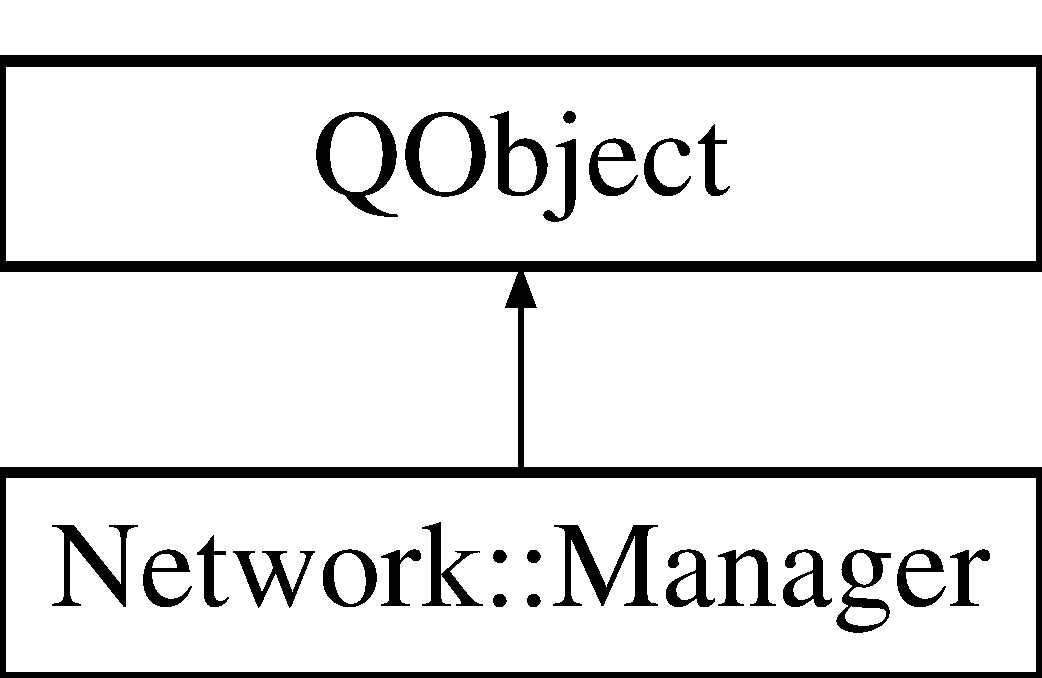
\includegraphics[height=2.000000cm]{classNetwork_1_1Manager}
\end{center}
\end{figure}
\subsection*{Public Slots}
\begin{DoxyCompactItemize}
\item 
\mbox{\Hypertarget{classNetwork_1_1Manager_aa8df583727aa598ee39e6de18b438abe}\label{classNetwork_1_1Manager_aa8df583727aa598ee39e6de18b438abe}} 
void {\bfseries get\+Resource} (const Q\+Url \&url)
\item 
\mbox{\Hypertarget{classNetwork_1_1Manager_a88e7de8604594cf6c2689e8b7a0a6e6e}\label{classNetwork_1_1Manager_a88e7de8604594cf6c2689e8b7a0a6e6e}} 
void {\bfseries post\+Resource} (const Q\+Url \&url, const Q\+Byte\+Array \&data)
\item 
\mbox{\Hypertarget{classNetwork_1_1Manager_adef1a35e5066157068800847c9366c09}\label{classNetwork_1_1Manager_adef1a35e5066157068800847c9366c09}} 
void {\bfseries delete\+Resource} (const Q\+Url \&url)
\item 
\mbox{\Hypertarget{classNetwork_1_1Manager_a42ef9df33cf238b62e66a5759c316432}\label{classNetwork_1_1Manager_a42ef9df33cf238b62e66a5759c316432}} 
void {\bfseries head\+Resource} (const Q\+Url \&url)
\end{DoxyCompactItemize}
\subsection*{Signals}
\begin{DoxyCompactItemize}
\item 
\mbox{\Hypertarget{classNetwork_1_1Manager_a1863c9a52ea6587387c8a688b92a2204}\label{classNetwork_1_1Manager_a1863c9a52ea6587387c8a688b92a2204}} 
void {\bfseries request\+Completed} (Q\+Network\+Reply $\ast$reply)
\item 
\mbox{\Hypertarget{classNetwork_1_1Manager_a4fd0af58f8fcd61b2c17d2dd368693c6}\label{classNetwork_1_1Manager_a4fd0af58f8fcd61b2c17d2dd368693c6}} 
Q\+List$<$ Q\+Ssl\+Error $>$ {\bfseries ssl\+Errors\+Received} (Q\+Network\+Reply $\ast$reply, Q\+List$<$ Q\+Ssl\+Error $>$ ssl\+Error)
\item 
\mbox{\Hypertarget{classNetwork_1_1Manager_a39de38077117c92e1e9d6aea325b9537}\label{classNetwork_1_1Manager_a39de38077117c92e1e9d6aea325b9537}} 
Q\+Network\+Access\+Manager\+::\+Network\+Accessibility {\bfseries network\+Accessible\+Changed} (Q\+Network\+Access\+Manager\+::\+Network\+Accessibility state)
\item 
\mbox{\Hypertarget{classNetwork_1_1Manager_ad8dd2cecf77ca5869e46b4268e6e0c9a}\label{classNetwork_1_1Manager_ad8dd2cecf77ca5869e46b4268e6e0c9a}} 
void {\bfseries user\+Agent\+Changed} ()
\item 
\mbox{\Hypertarget{classNetwork_1_1Manager_a1f37b9f5fe58a613d5095893e7c9ddb7}\label{classNetwork_1_1Manager_a1f37b9f5fe58a613d5095893e7c9ddb7}} 
void {\bfseries accept\+Header\+Changed} ()
\end{DoxyCompactItemize}
\subsection*{Public Member Functions}
\begin{DoxyCompactItemize}
\item 
\mbox{\Hypertarget{classNetwork_1_1Manager_aa4f7e5630c9c95932146f0f97eb38ca1}\label{classNetwork_1_1Manager_aa4f7e5630c9c95932146f0f97eb38ca1}} 
Q\+String {\bfseries user\+Agent} () const
\item 
\mbox{\Hypertarget{classNetwork_1_1Manager_acb21aaf997144be186e7e07043cd04ba}\label{classNetwork_1_1Manager_acb21aaf997144be186e7e07043cd04ba}} 
void {\bfseries set\+User\+Agent} (const Q\+String \&user\+Agent)
\item 
\mbox{\Hypertarget{classNetwork_1_1Manager_ac0db9092d325d920fff7a2d095cf506b}\label{classNetwork_1_1Manager_ac0db9092d325d920fff7a2d095cf506b}} 
Q\+String {\bfseries accept\+Header} () const
\item 
\mbox{\Hypertarget{classNetwork_1_1Manager_ab2c4f941034a92beae89f5657777f992}\label{classNetwork_1_1Manager_ab2c4f941034a92beae89f5657777f992}} 
void {\bfseries set\+Accept\+Header} (const Q\+String \&accept\+Header)
\end{DoxyCompactItemize}
\subsection*{Static Public Member Functions}
\begin{DoxyCompactItemize}
\item 
\mbox{\Hypertarget{classNetwork_1_1Manager_adeda284a39ae4c942656ec87295cf024}\label{classNetwork_1_1Manager_adeda284a39ae4c942656ec87295cf024}} 
static \mbox{\hyperlink{classNetwork_1_1Manager}{Manager}} $\ast$ {\bfseries get\+Instance} ()
\end{DoxyCompactItemize}
\subsection*{Private Member Functions}
\begin{DoxyCompactItemize}
\item 
\mbox{\Hypertarget{classNetwork_1_1Manager_ad3499eea3fd823034264277f9e0cf6a9}\label{classNetwork_1_1Manager_ad3499eea3fd823034264277f9e0cf6a9}} 
{\bfseries Manager} (Q\+Object $\ast$parent=nullptr)
\item 
\mbox{\Hypertarget{classNetwork_1_1Manager_aa9c1081a6e3ec9b937c3bbb9a7f7202f}\label{classNetwork_1_1Manager_aa9c1081a6e3ec9b937c3bbb9a7f7202f}} 
Q\+Network\+Request {\bfseries prepare\+Request} (const Q\+Url \&url)
\item 
\mbox{\Hypertarget{classNetwork_1_1Manager_a105b541b83fa32472b40730a885154ef}\label{classNetwork_1_1Manager_a105b541b83fa32472b40730a885154ef}} 
Q\+Network\+Access\+Manager $\ast$ {\bfseries Q\+N\+AM} () const
\item 
\mbox{\Hypertarget{classNetwork_1_1Manager_aaf5a945f52e51e357b53cacdc7319ab2}\label{classNetwork_1_1Manager_aaf5a945f52e51e357b53cacdc7319ab2}} 
void {\bfseries set\+Q\+N\+AM} (Q\+Network\+Access\+Manager $\ast$value)
\item 
\mbox{\Hypertarget{classNetwork_1_1Manager_a4aea14959afca0afd4b91208033da401}\label{classNetwork_1_1Manager_a4aea14959afca0afd4b91208033da401}} 
Q\+Abstract\+Network\+Cache $\ast$ {\bfseries cache} () const
\item 
\mbox{\Hypertarget{classNetwork_1_1Manager_ab73570326de530e3cdd09f6bf3f195d0}\label{classNetwork_1_1Manager_ab73570326de530e3cdd09f6bf3f195d0}} 
void {\bfseries set\+Cache} (Q\+Abstract\+Network\+Cache $\ast$cache)
\end{DoxyCompactItemize}
\subsection*{Static Private Member Functions}
\begin{DoxyCompactItemize}
\item 
\mbox{\Hypertarget{classNetwork_1_1Manager_a42c71474900c4d1e68740ae8d73db848}\label{classNetwork_1_1Manager_a42c71474900c4d1e68740ae8d73db848}} 
static \mbox{\hyperlink{classNetwork_1_1Manager}{Manager}} $\ast$ {\bfseries manager} ()
\item 
\mbox{\Hypertarget{classNetwork_1_1Manager_a1bc97c8b2dc5a4be751005d6a5dcf0a0}\label{classNetwork_1_1Manager_a1bc97c8b2dc5a4be751005d6a5dcf0a0}} 
static void {\bfseries set\+Manager} (const \mbox{\hyperlink{classNetwork_1_1Manager}{Manager}} $\ast$manager)
\end{DoxyCompactItemize}
\subsection*{Private Attributes}
\begin{DoxyCompactItemize}
\item 
\mbox{\Hypertarget{classNetwork_1_1Manager_a6f69f8099c8706abebd1a4497e5038f8}\label{classNetwork_1_1Manager_a6f69f8099c8706abebd1a4497e5038f8}} 
Q\+Network\+Access\+Manager $\ast$ {\bfseries m\+\_\+\+Q\+N\+AM}
\item 
\mbox{\Hypertarget{classNetwork_1_1Manager_aa99fb56d9b2a75b5f5a63a191002f461}\label{classNetwork_1_1Manager_aa99fb56d9b2a75b5f5a63a191002f461}} 
Q\+Abstract\+Network\+Cache $\ast$ {\bfseries m\+\_\+cache}
\item 
\mbox{\Hypertarget{classNetwork_1_1Manager_a59e8c58e1efd376525f400750ee87943}\label{classNetwork_1_1Manager_a59e8c58e1efd376525f400750ee87943}} 
Q\+String {\bfseries m\+\_\+user\+Agent}
\item 
\mbox{\Hypertarget{classNetwork_1_1Manager_a04138b3a1b6b6d9a0c8816de74ab50a2}\label{classNetwork_1_1Manager_a04138b3a1b6b6d9a0c8816de74ab50a2}} 
Q\+String {\bfseries m\+\_\+accept\+Header}
\end{DoxyCompactItemize}
\subsection*{Static Private Attributes}
\begin{DoxyCompactItemize}
\item 
\mbox{\Hypertarget{classNetwork_1_1Manager_a02ab401c85b17ffca2b9f3f69a4bae3b}\label{classNetwork_1_1Manager_a02ab401c85b17ffca2b9f3f69a4bae3b}} 
static \mbox{\hyperlink{classNetwork_1_1Manager}{Manager}} $\ast$ {\bfseries m\+\_\+instance} = nullptr
\end{DoxyCompactItemize}


The documentation for this class was generated from the following files\+:\begin{DoxyCompactItemize}
\item 
src/include/network/networkmanager.\+h\item 
src/network/\mbox{\hyperlink{networkmanager_8cpp}{networkmanager.\+cpp}}\end{DoxyCompactItemize}

\hypertarget{classDatabase_1_1Manager}{}\section{Database\+:\+:Manager Class Reference}
\label{classDatabase_1_1Manager}\index{Database\+::\+Manager@{Database\+::\+Manager}}


{\ttfamily \#include $<$databasemanager.\+h$>$}

Inheritance diagram for Database\+:\+:Manager\+:\begin{figure}[H]
\begin{center}
\leavevmode
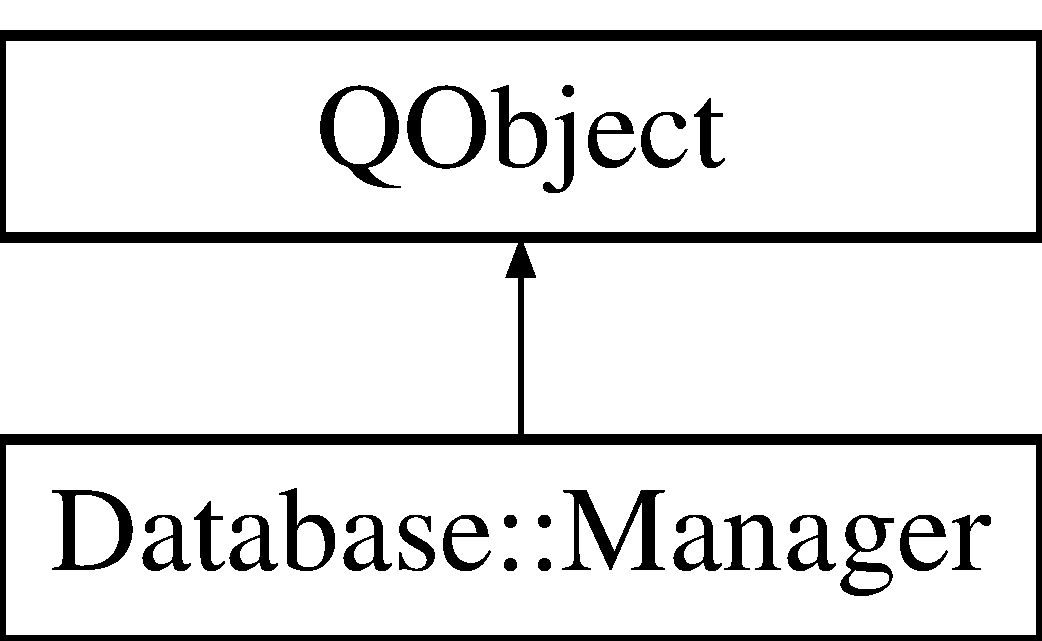
\includegraphics[height=2.000000cm]{classDatabase_1_1Manager}
\end{center}
\end{figure}
\subsection*{Public Member Functions}
\begin{DoxyCompactItemize}
\item 
bool \mbox{\hyperlink{classDatabase_1_1Manager_a0afd7a0884097a8dcff61b0444f39fb4}{execute}} (Q\+Sql\+Query \&query)
\item 
bool \mbox{\hyperlink{classDatabase_1_1Manager_adbe8be75b47c9770556464859bcc3017}{start\+Transaction}} ()
\item 
bool \mbox{\hyperlink{classDatabase_1_1Manager_a08dc190a448c555f8334bdd60d32b26e}{end\+Transaction}} ()
\item 
Q\+Sql\+Database \mbox{\hyperlink{classDatabase_1_1Manager_aecc5a00737bf6392cccda37a99138d8c}{database}} () const
\end{DoxyCompactItemize}
\subsection*{Static Public Member Functions}
\begin{DoxyCompactItemize}
\item 
static \mbox{\hyperlink{classDatabase_1_1Manager}{Manager}} $\ast$ \mbox{\hyperlink{classDatabase_1_1Manager_a6f8f8635c67e8d6e3ee86410006d22f3}{get\+Instance}} (const Q\+String \&path, Q\+Object $\ast$parent=nullptr)
\end{DoxyCompactItemize}
\subsection*{Private Member Functions}
\begin{DoxyCompactItemize}
\item 
\mbox{\hyperlink{classDatabase_1_1Manager_a3046834f78e2c3c5bce479b8eba31df4}{Manager}} (const Q\+String \&path, Q\+Object $\ast$parent)
\item 
void \mbox{\hyperlink{classDatabase_1_1Manager_af7f86ed5807bd6299fe4aa594b72013c}{set\+Database}} (const Q\+Sql\+Database \&\mbox{\hyperlink{classDatabase_1_1Manager_aecc5a00737bf6392cccda37a99138d8c}{database}})
\end{DoxyCompactItemize}
\subsection*{Private Attributes}
\begin{DoxyCompactItemize}
\item 
Q\+Sql\+Database \mbox{\hyperlink{classDatabase_1_1Manager_a4de33edd790c0d8320c0a2a5990f5169}{m\+\_\+database}}
\end{DoxyCompactItemize}
\subsection*{Static Private Attributes}
\begin{DoxyCompactItemize}
\item 
static \mbox{\hyperlink{classDatabase_1_1Manager}{Manager}} $\ast$ \mbox{\hyperlink{classDatabase_1_1Manager_a35e8446687862c34ae818636f953f54e}{m\+\_\+instance}} = nullptr
\end{DoxyCompactItemize}


\subsection{Constructor \& Destructor Documentation}
\mbox{\Hypertarget{classDatabase_1_1Manager_a3046834f78e2c3c5bce479b8eba31df4}\label{classDatabase_1_1Manager_a3046834f78e2c3c5bce479b8eba31df4}} 
\index{Database\+::\+Manager@{Database\+::\+Manager}!Manager@{Manager}}
\index{Manager@{Manager}!Database\+::\+Manager@{Database\+::\+Manager}}
\subsubsection{\texorpdfstring{Manager()}{Manager()}}
{\footnotesize\ttfamily Database\+::\+Manager\+::\+Manager (\begin{DoxyParamCaption}\item[{const Q\+String \&}]{path,  }\item[{Q\+Object $\ast$}]{parent }\end{DoxyParamCaption})\hspace{0.3cm}{\ttfamily [explicit]}, {\ttfamily [private]}}



\subsection{Member Function Documentation}
\mbox{\Hypertarget{classDatabase_1_1Manager_aecc5a00737bf6392cccda37a99138d8c}\label{classDatabase_1_1Manager_aecc5a00737bf6392cccda37a99138d8c}} 
\index{Database\+::\+Manager@{Database\+::\+Manager}!database@{database}}
\index{database@{database}!Database\+::\+Manager@{Database\+::\+Manager}}
\subsubsection{\texorpdfstring{database()}{database()}}
{\footnotesize\ttfamily Q\+Sql\+Database Database\+::\+Manager\+::database (\begin{DoxyParamCaption}{ }\end{DoxyParamCaption}) const}

\mbox{\Hypertarget{classDatabase_1_1Manager_a08dc190a448c555f8334bdd60d32b26e}\label{classDatabase_1_1Manager_a08dc190a448c555f8334bdd60d32b26e}} 
\index{Database\+::\+Manager@{Database\+::\+Manager}!end\+Transaction@{end\+Transaction}}
\index{end\+Transaction@{end\+Transaction}!Database\+::\+Manager@{Database\+::\+Manager}}
\subsubsection{\texorpdfstring{end\+Transaction()}{endTransaction()}}
{\footnotesize\ttfamily bool Database\+::\+Manager\+::end\+Transaction (\begin{DoxyParamCaption}{ }\end{DoxyParamCaption})}

\mbox{\Hypertarget{classDatabase_1_1Manager_a0afd7a0884097a8dcff61b0444f39fb4}\label{classDatabase_1_1Manager_a0afd7a0884097a8dcff61b0444f39fb4}} 
\index{Database\+::\+Manager@{Database\+::\+Manager}!execute@{execute}}
\index{execute@{execute}!Database\+::\+Manager@{Database\+::\+Manager}}
\subsubsection{\texorpdfstring{execute()}{execute()}}
{\footnotesize\ttfamily bool Database\+::\+Manager\+::execute (\begin{DoxyParamCaption}\item[{Q\+Sql\+Query \&}]{query }\end{DoxyParamCaption})}

\mbox{\Hypertarget{classDatabase_1_1Manager_a6f8f8635c67e8d6e3ee86410006d22f3}\label{classDatabase_1_1Manager_a6f8f8635c67e8d6e3ee86410006d22f3}} 
\index{Database\+::\+Manager@{Database\+::\+Manager}!get\+Instance@{get\+Instance}}
\index{get\+Instance@{get\+Instance}!Database\+::\+Manager@{Database\+::\+Manager}}
\subsubsection{\texorpdfstring{get\+Instance()}{getInstance()}}
{\footnotesize\ttfamily \mbox{\hyperlink{classDatabase_1_1Manager}{Database\+::\+Manager}} $\ast$ Database\+::\+Manager\+::get\+Instance (\begin{DoxyParamCaption}\item[{const Q\+String \&}]{path,  }\item[{Q\+Object $\ast$}]{parent = {\ttfamily nullptr} }\end{DoxyParamCaption})\hspace{0.3cm}{\ttfamily [static]}}

\mbox{\Hypertarget{classDatabase_1_1Manager_af7f86ed5807bd6299fe4aa594b72013c}\label{classDatabase_1_1Manager_af7f86ed5807bd6299fe4aa594b72013c}} 
\index{Database\+::\+Manager@{Database\+::\+Manager}!set\+Database@{set\+Database}}
\index{set\+Database@{set\+Database}!Database\+::\+Manager@{Database\+::\+Manager}}
\subsubsection{\texorpdfstring{set\+Database()}{setDatabase()}}
{\footnotesize\ttfamily void Database\+::\+Manager\+::set\+Database (\begin{DoxyParamCaption}\item[{const Q\+Sql\+Database \&}]{database }\end{DoxyParamCaption})\hspace{0.3cm}{\ttfamily [private]}}

\mbox{\Hypertarget{classDatabase_1_1Manager_adbe8be75b47c9770556464859bcc3017}\label{classDatabase_1_1Manager_adbe8be75b47c9770556464859bcc3017}} 
\index{Database\+::\+Manager@{Database\+::\+Manager}!start\+Transaction@{start\+Transaction}}
\index{start\+Transaction@{start\+Transaction}!Database\+::\+Manager@{Database\+::\+Manager}}
\subsubsection{\texorpdfstring{start\+Transaction()}{startTransaction()}}
{\footnotesize\ttfamily bool Database\+::\+Manager\+::start\+Transaction (\begin{DoxyParamCaption}{ }\end{DoxyParamCaption})}



\subsection{Member Data Documentation}
\mbox{\Hypertarget{classDatabase_1_1Manager_a4de33edd790c0d8320c0a2a5990f5169}\label{classDatabase_1_1Manager_a4de33edd790c0d8320c0a2a5990f5169}} 
\index{Database\+::\+Manager@{Database\+::\+Manager}!m\+\_\+database@{m\+\_\+database}}
\index{m\+\_\+database@{m\+\_\+database}!Database\+::\+Manager@{Database\+::\+Manager}}
\subsubsection{\texorpdfstring{m\+\_\+database}{m\_database}}
{\footnotesize\ttfamily Q\+Sql\+Database Database\+::\+Manager\+::m\+\_\+database\hspace{0.3cm}{\ttfamily [private]}}

\mbox{\Hypertarget{classDatabase_1_1Manager_a35e8446687862c34ae818636f953f54e}\label{classDatabase_1_1Manager_a35e8446687862c34ae818636f953f54e}} 
\index{Database\+::\+Manager@{Database\+::\+Manager}!m\+\_\+instance@{m\+\_\+instance}}
\index{m\+\_\+instance@{m\+\_\+instance}!Database\+::\+Manager@{Database\+::\+Manager}}
\subsubsection{\texorpdfstring{m\+\_\+instance}{m\_instance}}
{\footnotesize\ttfamily \mbox{\hyperlink{classDatabase_1_1Manager}{Database\+::\+Manager}} $\ast$ Database\+::\+Manager\+::m\+\_\+instance = nullptr\hspace{0.3cm}{\ttfamily [static]}, {\ttfamily [private]}}



The documentation for this class was generated from the following files\+:\begin{DoxyCompactItemize}
\item 
src/database/\mbox{\hyperlink{databasemanager_8h}{databasemanager.\+h}}\item 
src/database/\mbox{\hyperlink{databasemanager_8cpp}{databasemanager.\+cpp}}\end{DoxyCompactItemize}

\hypertarget{classAlertsEngine_1_1Message}{}\section{Alerts\+Engine\+:\+:Message Class Reference}
\label{classAlertsEngine_1_1Message}\index{Alerts\+Engine\+::\+Message@{Alerts\+Engine\+::\+Message}}
Inheritance diagram for Alerts\+Engine\+:\+:Message\+:\begin{figure}[H]
\begin{center}
\leavevmode
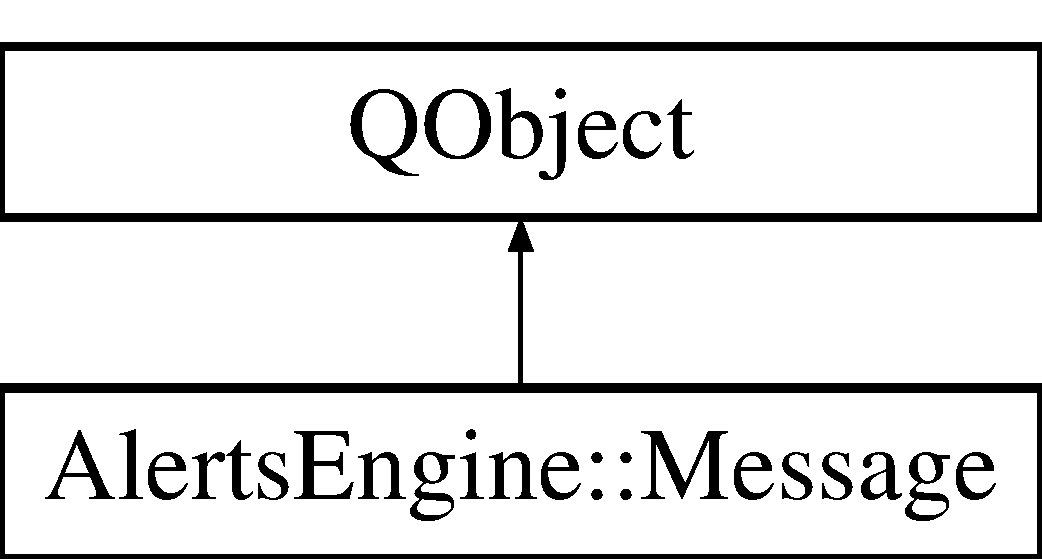
\includegraphics[height=2.000000cm]{classAlertsEngine_1_1Message}
\end{center}
\end{figure}
\subsection*{Signals}
\begin{DoxyCompactItemize}
\item 
\mbox{\Hypertarget{classAlertsEngine_1_1Message_a3473a72eeb26ff623481efc13018c846}\label{classAlertsEngine_1_1Message_a3473a72eeb26ff623481efc13018c846}} 
void {\bfseries header\+Changed} ()
\item 
\mbox{\Hypertarget{classAlertsEngine_1_1Message_a0064ac8f44048fd34f1c53a7d64af58f}\label{classAlertsEngine_1_1Message_a0064ac8f44048fd34f1c53a7d64af58f}} 
void {\bfseries description\+Changed} ()
\item 
\mbox{\Hypertarget{classAlertsEngine_1_1Message_af268d538b313ac7f625c98de03d6389f}\label{classAlertsEngine_1_1Message_af268d538b313ac7f625c98de03d6389f}} 
void {\bfseries lead\+Changed} ()
\item 
\mbox{\Hypertarget{classAlertsEngine_1_1Message_a6010da9ca6fd506cb12b2b4ba9459aeb}\label{classAlertsEngine_1_1Message_a6010da9ca6fd506cb12b2b4ba9459aeb}} 
void {\bfseries link\+Changed} ()
\end{DoxyCompactItemize}
\subsection*{Public Member Functions}
\begin{DoxyCompactItemize}
\item 
\mbox{\Hypertarget{classAlertsEngine_1_1Message_aa5678fba37f1eb3917b639dba45649bd}\label{classAlertsEngine_1_1Message_aa5678fba37f1eb3917b639dba45649bd}} 
{\bfseries Message} (const Q\+String \&header, const Q\+String \&description, const Q\+String \&lead, const Q\+Url \&link, Q\+Object $\ast$parent=nullptr)
\item 
\mbox{\Hypertarget{classAlertsEngine_1_1Message_a5cd29b13fa9414b81b40746f13c8a8f6}\label{classAlertsEngine_1_1Message_a5cd29b13fa9414b81b40746f13c8a8f6}} 
{\bfseries Message} (const Q\+String \&header, const Q\+String \&description, Q\+Object $\ast$parent=nullptr)
\item 
\mbox{\Hypertarget{classAlertsEngine_1_1Message_abe2167f76ca26a33049b9c4161bb3f70}\label{classAlertsEngine_1_1Message_abe2167f76ca26a33049b9c4161bb3f70}} 
Q\+String {\bfseries header} () const
\item 
\mbox{\Hypertarget{classAlertsEngine_1_1Message_a1b6364415df2677d4f2f97ba4a60fbc6}\label{classAlertsEngine_1_1Message_a1b6364415df2677d4f2f97ba4a60fbc6}} 
void {\bfseries set\+Header} (const Q\+String \&header)
\item 
\mbox{\Hypertarget{classAlertsEngine_1_1Message_a9179c8055fbaf7dc8d435831dd22faab}\label{classAlertsEngine_1_1Message_a9179c8055fbaf7dc8d435831dd22faab}} 
Q\+String {\bfseries description} () const
\item 
\mbox{\Hypertarget{classAlertsEngine_1_1Message_ac06351f3c3e17a03f6ee34e9c2a24752}\label{classAlertsEngine_1_1Message_ac06351f3c3e17a03f6ee34e9c2a24752}} 
void {\bfseries set\+Description} (const Q\+String \&description)
\item 
\mbox{\Hypertarget{classAlertsEngine_1_1Message_a5a1769dd0d4add541246bab3c33b4008}\label{classAlertsEngine_1_1Message_a5a1769dd0d4add541246bab3c33b4008}} 
Q\+String {\bfseries lead} () const
\item 
\mbox{\Hypertarget{classAlertsEngine_1_1Message_a5ded2d853725b517bda49bdae59f26ee}\label{classAlertsEngine_1_1Message_a5ded2d853725b517bda49bdae59f26ee}} 
void {\bfseries set\+Lead} (const Q\+String \&lead)
\item 
\mbox{\Hypertarget{classAlertsEngine_1_1Message_aea81d49a5b776d58e9dbee8ac1708e84}\label{classAlertsEngine_1_1Message_aea81d49a5b776d58e9dbee8ac1708e84}} 
Q\+Url {\bfseries link} () const
\item 
\mbox{\Hypertarget{classAlertsEngine_1_1Message_a1a8aaf9ec0c56af40d418318e0340b54}\label{classAlertsEngine_1_1Message_a1a8aaf9ec0c56af40d418318e0340b54}} 
void {\bfseries set\+Link} (const Q\+Url \&link)
\end{DoxyCompactItemize}
\subsection*{Private Attributes}
\begin{DoxyCompactItemize}
\item 
\mbox{\Hypertarget{classAlertsEngine_1_1Message_ad6a3061911f65418a0d3b47f4e296cfd}\label{classAlertsEngine_1_1Message_ad6a3061911f65418a0d3b47f4e296cfd}} 
Q\+String {\bfseries m\+\_\+header}
\item 
\mbox{\Hypertarget{classAlertsEngine_1_1Message_ac5e8f3c8cd7c891ff82113cbc29573b3}\label{classAlertsEngine_1_1Message_ac5e8f3c8cd7c891ff82113cbc29573b3}} 
Q\+String {\bfseries m\+\_\+description}
\item 
\mbox{\Hypertarget{classAlertsEngine_1_1Message_a6bff02029f8c7ecbf7f6d0d921a39f05}\label{classAlertsEngine_1_1Message_a6bff02029f8c7ecbf7f6d0d921a39f05}} 
Q\+String {\bfseries m\+\_\+lead}
\item 
\mbox{\Hypertarget{classAlertsEngine_1_1Message_ab45be7942acc34c94047983a43ab8340}\label{classAlertsEngine_1_1Message_ab45be7942acc34c94047983a43ab8340}} 
Q\+Url {\bfseries m\+\_\+link}
\end{DoxyCompactItemize}


The documentation for this class was generated from the following files\+:\begin{DoxyCompactItemize}
\item 
src/include/engines/alerts/alertsmessage.\+h\item 
src/engines/alerts/\mbox{\hyperlink{alertsmessage_8cpp}{alertsmessage.\+cpp}}\end{DoxyCompactItemize}

\hypertarget{classStationEngine_1_1NullStation}{}\section{Station\+Engine\+:\+:Null\+Station Class Reference}
\label{classStationEngine_1_1NullStation}\index{Station\+Engine\+::\+Null\+Station@{Station\+Engine\+::\+Null\+Station}}
Inheritance diagram for Station\+Engine\+:\+:Null\+Station\+:\begin{figure}[H]
\begin{center}
\leavevmode
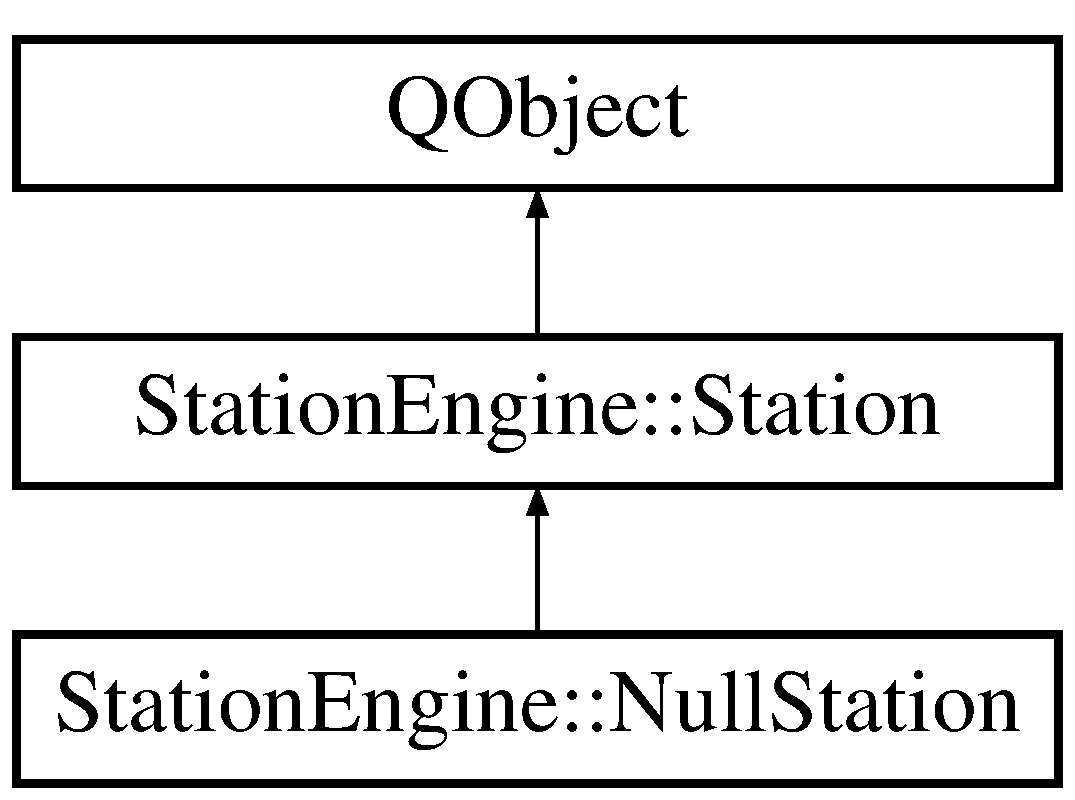
\includegraphics[height=3.000000cm]{classStationEngine_1_1NullStation}
\end{center}
\end{figure}
\subsection*{Static Public Member Functions}
\begin{DoxyCompactItemize}
\item 
\mbox{\Hypertarget{classStationEngine_1_1NullStation_a620d1cc84bf91ad1c2cadf1f810c9832}\label{classStationEngine_1_1NullStation_a620d1cc84bf91ad1c2cadf1f810c9832}} 
static \mbox{\hyperlink{classStationEngine_1_1NullStation}{Null\+Station}} $\ast$ {\bfseries get\+Instance} ()
\end{DoxyCompactItemize}
\subsection*{Private Member Functions}
\begin{DoxyCompactItemize}
\item 
\mbox{\Hypertarget{classStationEngine_1_1NullStation_a3fb4fcd10147e1b301c74c8391c1ab9b}\label{classStationEngine_1_1NullStation_a3fb4fcd10147e1b301c74c8391c1ab9b}} 
{\bfseries Null\+Station} (const Q\+Url \&uri, const Q\+Map$<$ Q\+Locale\+::\+Language, Q\+String $>$ \&name, const Q\+Locale\+::\+Country \&country, const Q\+Geo\+Coordinate \&position, const Q\+Geo\+Address \&address, const bool \&has\+Ticket\+Vending\+Machine, const bool \&has\+Luggage\+Lockers, const bool \&has\+Free\+Parking, const bool \&has\+Taxi, const bool \&has\+Bicycle\+Spots, const bool \&has\+Blue\+Bike, const bool \&has\+Bus, const bool \&has\+Tram, const bool \&has\+Metro, const bool \&has\+Wheelchair\+Available, const bool \&has\+Ramp, const qint16 \&disabled\+Parking\+Spots, const bool \&has\+Elevated\+Platform, const bool \&has\+Escalator\+Up, const bool \&has\+Escalator\+Down, const bool \&has\+Elevator\+Platform, const bool \&has\+Hearing\+Aid\+Signal, const Q\+Map$<$ Station\+Engine\+::\+Station\+::\+Day, Q\+Pair$<$ Q\+Time, Q\+Time $>$$>$ \&opening\+Hours, const qreal \&average\+Stop\+Times, Q\+Object $\ast$parent=nullptr)
\end{DoxyCompactItemize}
\subsection*{Static Private Attributes}
\begin{DoxyCompactItemize}
\item 
\mbox{\Hypertarget{classStationEngine_1_1NullStation_ab5a0e3840dc39b8e7e62c56c4847fbd3}\label{classStationEngine_1_1NullStation_ab5a0e3840dc39b8e7e62c56c4847fbd3}} 
static \mbox{\hyperlink{classStationEngine_1_1NullStation}{Station\+Engine\+::\+Null\+Station}} $\ast$ {\bfseries m\+\_\+instance} = nullptr
\end{DoxyCompactItemize}
\subsection*{Additional Inherited Members}


The documentation for this class was generated from the following files\+:\begin{DoxyCompactItemize}
\item 
src/include/engines/station/stationnullstation.\+h\item 
src/engines/station/stationnullstation.\+cpp\end{DoxyCompactItemize}

\hypertarget{classOS}{}\section{OS Class Reference}
\label{classOS}\index{OS@{OS}}
Inheritance diagram for OS\+:\begin{figure}[H]
\begin{center}
\leavevmode
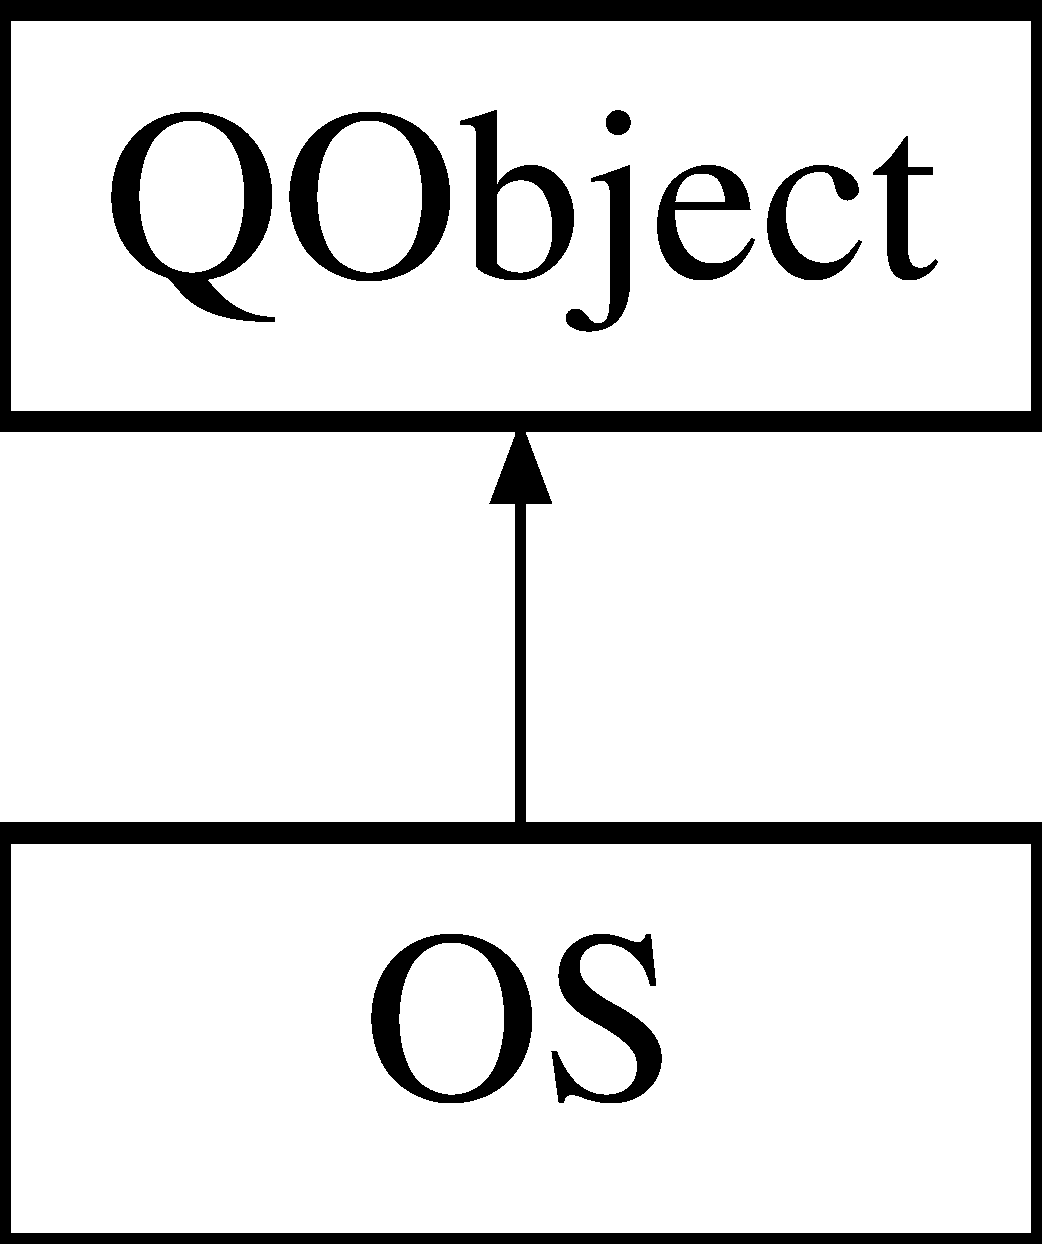
\includegraphics[height=2.000000cm]{classOS}
\end{center}
\end{figure}
\subsection*{Signals}
\begin{DoxyCompactItemize}
\item 
\mbox{\Hypertarget{classOS_a58369b88b24b1701b020bd0971d99c03}\label{classOS_a58369b88b24b1701b020bd0971d99c03}} 
void {\bfseries release\+Changed} ()
\item 
\mbox{\Hypertarget{classOS_a2bb282eb19c9eaa0c787dabc434a9fca}\label{classOS_a2bb282eb19c9eaa0c787dabc434a9fca}} 
void {\bfseries version\+Changed} ()
\item 
\mbox{\Hypertarget{classOS_ad55c57724a077d427b89ede6e1f8b235}\label{classOS_ad55c57724a077d427b89ede6e1f8b235}} 
void {\bfseries app\+Name\+Changed} ()
\item 
\mbox{\Hypertarget{classOS_a21d29e6b9eef2bccc62db0d29d56b4c5}\label{classOS_a21d29e6b9eef2bccc62db0d29d56b4c5}} 
void {\bfseries app\+Name\+Pretty\+Changed} ()
\item 
\mbox{\Hypertarget{classOS_a39f7a3688e008fde1008e6b7e5b5ebcb}\label{classOS_a39f7a3688e008fde1008e6b7e5b5ebcb}} 
void {\bfseries app\+Version\+Changed} ()
\item 
\mbox{\Hypertarget{classOS_a0ecbe56e6ec612ba6f78af5086505751}\label{classOS_a0ecbe56e6ec612ba6f78af5086505751}} 
void {\bfseries devicepixelratio\+Changed} ()
\end{DoxyCompactItemize}
\subsection*{Public Member Functions}
\begin{DoxyCompactItemize}
\item 
\mbox{\Hypertarget{classOS_ac21113cbcd347809f657c6a27a0278f6}\label{classOS_ac21113cbcd347809f657c6a27a0278f6}} 
Q\+\_\+\+I\+N\+V\+O\+K\+A\+B\+LE void {\bfseries create\+Notification} (Q\+String title, Q\+String text, Q\+String feedback, Q\+String category)
\item 
\mbox{\Hypertarget{classOS_a949a6aa1c2f8cd63d27cd6b8869da8fc}\label{classOS_a949a6aa1c2f8cd63d27cd6b8869da8fc}} 
Q\+\_\+\+I\+N\+V\+O\+K\+A\+B\+LE void {\bfseries create\+Toaster} (Q\+String text, Q\+String icon, Q\+String category)
\item 
\mbox{\Hypertarget{classOS_a8ab936784f48408f14ad73f10ae5afb8}\label{classOS_a8ab936784f48408f14ad73f10ae5afb8}} 
Q\+\_\+\+I\+N\+V\+O\+K\+A\+B\+LE void {\bfseries close\+Notification\+By\+Category} (Q\+String category)
\item 
\mbox{\Hypertarget{classOS_a8cc3c6824e01ae679819c8c3daf7842e}\label{classOS_a8cc3c6824e01ae679819c8c3daf7842e}} 
Q\+\_\+\+I\+N\+V\+O\+K\+A\+B\+LE void {\bfseries close\+Notification\+By\+Replaces\+Id} (Q\+String replaces\+Id)
\item 
\mbox{\Hypertarget{classOS_a16c6da56d519e2c2bccbdeaf5c4ff29b}\label{classOS_a16c6da56d519e2c2bccbdeaf5c4ff29b}} 
Q\+\_\+\+I\+N\+V\+O\+K\+A\+B\+LE void {\bfseries close\+Notification\+All} ()
\item 
\mbox{\Hypertarget{classOS_a1d00cd418f5d83cc174492326f7cd604}\label{classOS_a1d00cd418f5d83cc174492326f7cd604}} 
Q\+String {\bfseries release} ()
\item 
\mbox{\Hypertarget{classOS_a4cd043becb244d8f40bdcc55c0417a71}\label{classOS_a4cd043becb244d8f40bdcc55c0417a71}} 
Q\+String {\bfseries version} ()
\item 
\mbox{\Hypertarget{classOS_a800e819bbb7aa20945893d138b2a1bb3}\label{classOS_a800e819bbb7aa20945893d138b2a1bb3}} 
Q\+String {\bfseries device} ()
\item 
\mbox{\Hypertarget{classOS_a44dcb6a2ee199b111d98eb1e364bfef7}\label{classOS_a44dcb6a2ee199b111d98eb1e364bfef7}} 
Q\+String {\bfseries cache\+Location} ()
\item 
\mbox{\Hypertarget{classOS_ae8a69330410d1b615443920baa19cea7}\label{classOS_ae8a69330410d1b615443920baa19cea7}} 
Q\+String {\bfseries data\+Location} ()
\item 
\mbox{\Hypertarget{classOS_ae319d1766558e1a93f0d2736d7f898b2}\label{classOS_ae319d1766558e1a93f0d2736d7f898b2}} 
Q\+String {\bfseries config\+Location} ()
\item 
\mbox{\Hypertarget{classOS_afa7ce7d8541fbbd43d82f09f8662af44}\label{classOS_afa7ce7d8541fbbd43d82f09f8662af44}} 
Q\+String {\bfseries photo\+Location} ()
\item 
\mbox{\Hypertarget{classOS_a611cc2d2496f6974b5087e8e2d3085e6}\label{classOS_a611cc2d2496f6974b5087e8e2d3085e6}} 
Q\+String {\bfseries music\+Location} ()
\item 
\mbox{\Hypertarget{classOS_a88ba12fba1acd2557506942e0099634b}\label{classOS_a88ba12fba1acd2557506942e0099634b}} 
Q\+String {\bfseries document\+Location} ()
\item 
\mbox{\Hypertarget{classOS_afdfd88fe0b70d4ed51508e7dc364b1d4}\label{classOS_afdfd88fe0b70d4ed51508e7dc364b1d4}} 
Q\+String {\bfseries video\+Location} ()
\item 
\mbox{\Hypertarget{classOS_a0dac0a86aca0d89d27b9596999506713}\label{classOS_a0dac0a86aca0d89d27b9596999506713}} 
Q\+String {\bfseries download\+Location} ()
\item 
\mbox{\Hypertarget{classOS_a5f0bcd7c973d5875be519ec3a06629f2}\label{classOS_a5f0bcd7c973d5875be519ec3a06629f2}} 
Q\+String {\bfseries log\+Location} ()
\item 
\mbox{\Hypertarget{classOS_a85848812c46025d92b9a061df85d9bce}\label{classOS_a85848812c46025d92b9a061df85d9bce}} 
Q\+String {\bfseries log\+File} ()
\item 
\mbox{\Hypertarget{classOS_a414805ecb488dd84a111fb2c8c6b9401}\label{classOS_a414805ecb488dd84a111fb2c8c6b9401}} 
Q\+String {\bfseries app\+Name} ()
\item 
\mbox{\Hypertarget{classOS_af545da4fea44bc32a873f7021498b9fc}\label{classOS_af545da4fea44bc32a873f7021498b9fc}} 
Q\+String {\bfseries app\+Name\+Pretty} ()
\item 
\mbox{\Hypertarget{classOS_ad216acfae668255c7e307e965e5e3a50}\label{classOS_ad216acfae668255c7e307e965e5e3a50}} 
Q\+String {\bfseries app\+Version} ()
\item 
\mbox{\Hypertarget{classOS_abec33b96eb8c7def86f6f918dc1849c0}\label{classOS_abec33b96eb8c7def86f6f918dc1849c0}} 
qreal {\bfseries devicepixelratio} ()
\end{DoxyCompactItemize}
\subsection*{Properties}
\begin{DoxyCompactItemize}
\item 
\mbox{\Hypertarget{classOS_ac78395d05ca770df0e6136dca18cf682}\label{classOS_ac78395d05ca770df0e6136dca18cf682}} 
Q\+String {\bfseries release}
\item 
\mbox{\Hypertarget{classOS_af9d3ad8c99dd34d874634eae3163dcc3}\label{classOS_af9d3ad8c99dd34d874634eae3163dcc3}} 
Q\+String {\bfseries version}
\item 
\mbox{\Hypertarget{classOS_af9d6295c5361884c9c7c25b13db70720}\label{classOS_af9d6295c5361884c9c7c25b13db70720}} 
Q\+String {\bfseries app\+Name}
\item 
\mbox{\Hypertarget{classOS_a5ecf65ef8f4ac491323d1590c2cb4e67}\label{classOS_a5ecf65ef8f4ac491323d1590c2cb4e67}} 
Q\+String {\bfseries app\+Name\+Pretty}
\item 
\mbox{\Hypertarget{classOS_a8162949b8a268b409967ae356947e059}\label{classOS_a8162949b8a268b409967ae356947e059}} 
Q\+String {\bfseries app\+Version}
\item 
\mbox{\Hypertarget{classOS_aa40d035f4f4b1f67c6c103cd3b3cfc08}\label{classOS_aa40d035f4f4b1f67c6c103cd3b3cfc08}} 
Q\+String {\bfseries devicepixelratio}
\end{DoxyCompactItemize}
\subsection*{Private Member Functions}
\begin{DoxyCompactItemize}
\item 
\mbox{\Hypertarget{classOS_a5703fdddfbee21d53e71906d509df442}\label{classOS_a5703fdddfbee21d53e71906d509df442}} 
Q\+List$<$ Q\+Pair$<$ Q\+String, Q\+String $>$ $>$ {\bfseries extract\+File\+Data} (Q\+String location, Q\+String\+List querry\+List)
\end{DoxyCompactItemize}
\subsection*{Private Attributes}
\begin{DoxyCompactItemize}
\item 
\mbox{\Hypertarget{classOS_a61a80d72fb7d8be61c14a0363e81176a}\label{classOS_a61a80d72fb7d8be61c14a0363e81176a}} 
Q\+String {\bfseries m\+\_\+release}
\item 
\mbox{\Hypertarget{classOS_a483dfd8fcc3c9e240f05638f01c697fa}\label{classOS_a483dfd8fcc3c9e240f05638f01c697fa}} 
Q\+String {\bfseries m\+\_\+version}
\item 
\mbox{\Hypertarget{classOS_aae83217d6785449722cae783468cb6ba}\label{classOS_aae83217d6785449722cae783468cb6ba}} 
Q\+String {\bfseries m\+\_\+device}
\end{DoxyCompactItemize}


The documentation for this class was generated from the following files\+:\begin{DoxyCompactItemize}
\item 
src/os.\+h\item 
src/os.\+cpp\end{DoxyCompactItemize}

\hypertarget{classFragments_1_1Page}{}\section{Fragments\+:\+:Page Class Reference}
\label{classFragments_1_1Page}\index{Fragments\+::\+Page@{Fragments\+::\+Page}}
Inheritance diagram for Fragments\+:\+:Page\+:\begin{figure}[H]
\begin{center}
\leavevmode
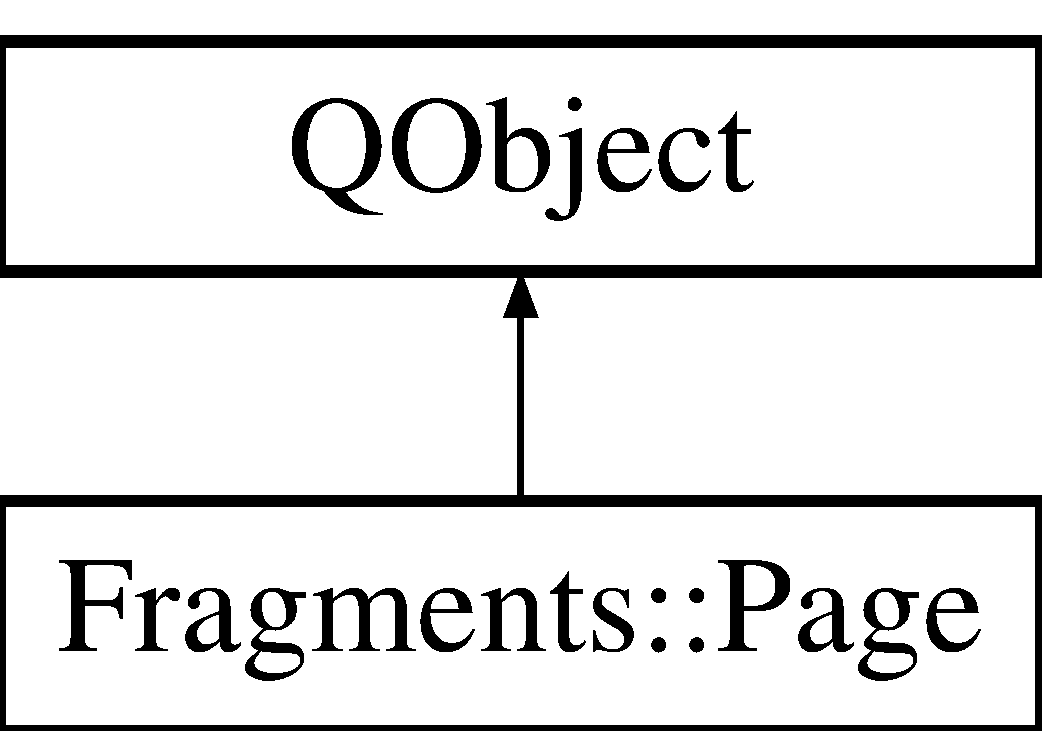
\includegraphics[height=2.000000cm]{classFragments_1_1Page}
\end{center}
\end{figure}
\subsection*{Signals}
\begin{DoxyCompactItemize}
\item 
\mbox{\Hypertarget{classFragments_1_1Page_a03f40d5c9520331432c9f1c7ab9f805c}\label{classFragments_1_1Page_a03f40d5c9520331432c9f1c7ab9f805c}} 
void {\bfseries uri\+Changed} ()
\item 
\mbox{\Hypertarget{classFragments_1_1Page_acfdd19abc8342361f975b4d9d10e2e64}\label{classFragments_1_1Page_acfdd19abc8342361f975b4d9d10e2e64}} 
void {\bfseries timestamp\+Changed} ()
\item 
\mbox{\Hypertarget{classFragments_1_1Page_a0b56ee63d18b43654cdfebd6a39c8d4f}\label{classFragments_1_1Page_a0b56ee63d18b43654cdfebd6a39c8d4f}} 
void {\bfseries hydra\+Next\+Changed} ()
\item 
\mbox{\Hypertarget{classFragments_1_1Page_a6f63a3428523cfa79ab30bfce32c0509}\label{classFragments_1_1Page_a6f63a3428523cfa79ab30bfce32c0509}} 
void {\bfseries hydra\+Previous\+Changed} ()
\item 
\mbox{\Hypertarget{classFragments_1_1Page_a6d449124d048af31d3e1e24a66c34636}\label{classFragments_1_1Page_a6d449124d048af31d3e1e24a66c34636}} 
void {\bfseries fragments\+Changed} ()
\end{DoxyCompactItemize}
\subsection*{Public Member Functions}
\begin{DoxyCompactItemize}
\item 
\mbox{\Hypertarget{classFragments_1_1Page_af61cfda59ee42caa75e373471ac91ae6}\label{classFragments_1_1Page_af61cfda59ee42caa75e373471ac91ae6}} 
{\bfseries Page} (Q\+Object $\ast$parent=nullptr)
\item 
\mbox{\Hypertarget{classFragments_1_1Page_ac345c0f46af8796c9f7fa702f71f240c}\label{classFragments_1_1Page_ac345c0f46af8796c9f7fa702f71f240c}} 
{\bfseries Page} (const Q\+Url \&uri, const Q\+Date\+Time \&timestamp, const Q\+Url \&hydra\+Next, const Q\+Url \&hydra\+Previous, const Q\+List$<$ \mbox{\hyperlink{classFragments_1_1Fragment}{Fragments\+::\+Fragment}} $\ast$$>$ \&fragments, Q\+Object $\ast$parent=nullptr)
\item 
\mbox{\Hypertarget{classFragments_1_1Page_a1185c1fb78c1d28eee03dba926fefcb8}\label{classFragments_1_1Page_a1185c1fb78c1d28eee03dba926fefcb8}} 
Q\+Url {\bfseries uri} () const
\item 
\mbox{\Hypertarget{classFragments_1_1Page_a13d34067ae20ee41b3003a6c2084fe2c}\label{classFragments_1_1Page_a13d34067ae20ee41b3003a6c2084fe2c}} 
void {\bfseries set\+U\+RI} (const Q\+Url \&uri)
\item 
\mbox{\Hypertarget{classFragments_1_1Page_a44cf4faf8776d3344bc4296d37b1f7ae}\label{classFragments_1_1Page_a44cf4faf8776d3344bc4296d37b1f7ae}} 
Q\+Date\+Time {\bfseries timestamp} () const
\item 
\mbox{\Hypertarget{classFragments_1_1Page_a5f771039432d7c46a7da56d34474bb8a}\label{classFragments_1_1Page_a5f771039432d7c46a7da56d34474bb8a}} 
void {\bfseries set\+Timestamp} (const Q\+Date\+Time \&timestamp)
\item 
\mbox{\Hypertarget{classFragments_1_1Page_a822bbc500bf1e5540582cdf258d73b20}\label{classFragments_1_1Page_a822bbc500bf1e5540582cdf258d73b20}} 
Q\+Url {\bfseries hydra\+Next} () const
\item 
\mbox{\Hypertarget{classFragments_1_1Page_a241195084d7c53ce0c8ad2fff67d9698}\label{classFragments_1_1Page_a241195084d7c53ce0c8ad2fff67d9698}} 
void {\bfseries set\+Hydra\+Next} (const Q\+Url \&hydra\+Next)
\item 
\mbox{\Hypertarget{classFragments_1_1Page_a102aada029299dbe7f8b55116eda0933}\label{classFragments_1_1Page_a102aada029299dbe7f8b55116eda0933}} 
Q\+Url {\bfseries hydra\+Previous} () const
\item 
\mbox{\Hypertarget{classFragments_1_1Page_a262f978bd4837db5e1c50b59a7984608}\label{classFragments_1_1Page_a262f978bd4837db5e1c50b59a7984608}} 
void {\bfseries set\+Hydra\+Previous} (const Q\+Url \&hydra\+Previous)
\item 
\mbox{\Hypertarget{classFragments_1_1Page_ab2460084209c3fe9211f70689ad78019}\label{classFragments_1_1Page_ab2460084209c3fe9211f70689ad78019}} 
Q\+List$<$ \mbox{\hyperlink{classFragments_1_1Fragment}{Fragments\+::\+Fragment}} $\ast$ $>$ {\bfseries fragments} () const
\item 
\mbox{\Hypertarget{classFragments_1_1Page_a41d271ad74d1aaf0b5de36d8619306f5}\label{classFragments_1_1Page_a41d271ad74d1aaf0b5de36d8619306f5}} 
void {\bfseries set\+Fragments} (const Q\+List$<$ \mbox{\hyperlink{classFragments_1_1Fragment}{Fragments\+::\+Fragment}} $\ast$$>$ \&fragments)
\end{DoxyCompactItemize}
\subsection*{Private Attributes}
\begin{DoxyCompactItemize}
\item 
\mbox{\Hypertarget{classFragments_1_1Page_ac674951355ab6c5e9c1aa7d8eeb7dbff}\label{classFragments_1_1Page_ac674951355ab6c5e9c1aa7d8eeb7dbff}} 
Q\+Url {\bfseries m\+\_\+uri}
\item 
\mbox{\Hypertarget{classFragments_1_1Page_a0bbe4f3dd97422b2e70936394fa755c6}\label{classFragments_1_1Page_a0bbe4f3dd97422b2e70936394fa755c6}} 
Q\+Date\+Time {\bfseries m\+\_\+timestamp}
\item 
\mbox{\Hypertarget{classFragments_1_1Page_aa6f58f42bfe8678444a170d1cbbe9902}\label{classFragments_1_1Page_aa6f58f42bfe8678444a170d1cbbe9902}} 
Q\+Url {\bfseries m\+\_\+hydra\+Next}
\item 
\mbox{\Hypertarget{classFragments_1_1Page_a3f6de09ddfb6d757b675f252c12bd4d8}\label{classFragments_1_1Page_a3f6de09ddfb6d757b675f252c12bd4d8}} 
Q\+Url {\bfseries m\+\_\+hydra\+Previous}
\item 
\mbox{\Hypertarget{classFragments_1_1Page_aac92876ae3e054b37430ee03b877d6b9}\label{classFragments_1_1Page_aac92876ae3e054b37430ee03b877d6b9}} 
Q\+List$<$ \mbox{\hyperlink{classFragments_1_1Fragment}{Fragments\+::\+Fragment}} $\ast$ $>$ {\bfseries m\+\_\+fragments}
\end{DoxyCompactItemize}


The documentation for this class was generated from the following files\+:\begin{DoxyCompactItemize}
\item 
src/include/fragments/fragmentspage.\+h\item 
src/fragments/\mbox{\hyperlink{fragmentspage_8cpp}{fragmentspage.\+cpp}}\end{DoxyCompactItemize}

\hypertarget{classRouterEngine_1_1Planner}{}\section{Router\+Engine\+:\+:Planner Class Reference}
\label{classRouterEngine_1_1Planner}\index{Router\+Engine\+::\+Planner@{Router\+Engine\+::\+Planner}}
Inheritance diagram for Router\+Engine\+:\+:Planner\+:\begin{figure}[H]
\begin{center}
\leavevmode
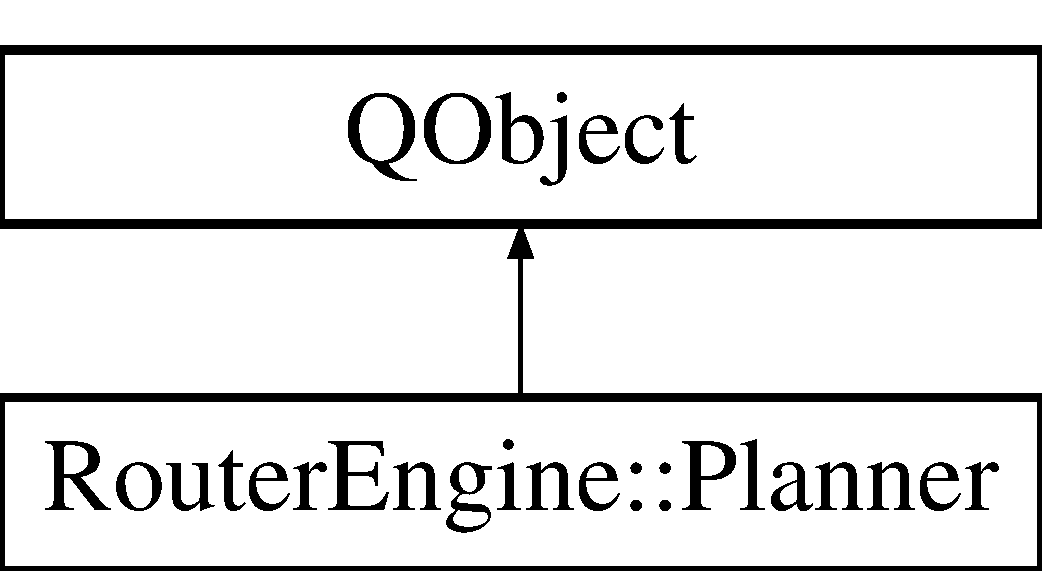
\includegraphics[height=2.000000cm]{classRouterEngine_1_1Planner}
\end{center}
\end{figure}
\subsection*{Signals}
\begin{DoxyCompactItemize}
\item 
\mbox{\Hypertarget{classRouterEngine_1_1Planner_a5c655efeb575e8842cf20bdd16fc025e}\label{classRouterEngine_1_1Planner_a5c655efeb575e8842cf20bdd16fc025e}} 
void {\bfseries routes\+Found} (const Q\+List$<$ \mbox{\hyperlink{classRouterEngine_1_1Route}{Router\+Engine\+::\+Route}} $\ast$$>$ \&routes)
\item 
\mbox{\Hypertarget{classRouterEngine_1_1Planner_a26d92d9ae44cdffae0e3b37765b1708e}\label{classRouterEngine_1_1Planner_a26d92d9ae44cdffae0e3b37765b1708e}} 
void {\bfseries error} (const Q\+String \&message)
\item 
\mbox{\Hypertarget{classRouterEngine_1_1Planner_ab4a2c861d1ed9561499a7036b809eb94}\label{classRouterEngine_1_1Planner_ab4a2c861d1ed9561499a7036b809eb94}} 
void {\bfseries page\+Requested} (const Q\+Url \&page\+U\+RI)
\item 
\mbox{\Hypertarget{classRouterEngine_1_1Planner_a081f70dd778700e47328330acffdbd6b}\label{classRouterEngine_1_1Planner_a081f70dd778700e47328330acffdbd6b}} 
void {\bfseries page\+Received} (const Q\+Url \&page\+U\+RI)
\item 
\mbox{\Hypertarget{classRouterEngine_1_1Planner_a64a706ca570771d9d9967a5288721219}\label{classRouterEngine_1_1Planner_a64a706ca570771d9d9967a5288721219}} 
void {\bfseries page\+Progress} (const Q\+Url \&page\+U\+RI, const qint16 \&progress)
\end{DoxyCompactItemize}
\subsection*{Public Member Functions}
\begin{DoxyCompactItemize}
\item 
\mbox{\Hypertarget{classRouterEngine_1_1Planner_ad4d13efc9958b6641489808b0bc2895e}\label{classRouterEngine_1_1Planner_ad4d13efc9958b6641489808b0bc2895e}} 
void {\bfseries get\+Connections} (const Q\+Url \&departure\+Station, const Q\+Url \&arrival\+Station, const Q\+Date\+Time \&departure\+Time, const qint16 \&max\+Transfers)
\item 
\mbox{\Hypertarget{classRouterEngine_1_1Planner_aabc46d28d07f0972ff20a41a69d11922}\label{classRouterEngine_1_1Planner_aabc46d28d07f0972ff20a41a69d11922}} 
Q\+Date\+Time {\bfseries calculate\+Arrival\+Time} (const Q\+Date\+Time \&departure\+Time)
\item 
\mbox{\Hypertarget{classRouterEngine_1_1Planner_aacb44fb55e948fd01378e7a8b5fe38dc}\label{classRouterEngine_1_1Planner_aacb44fb55e948fd01378e7a8b5fe38dc}} 
Q\+Date\+Time {\bfseries departure\+Time} () const
\item 
\mbox{\Hypertarget{classRouterEngine_1_1Planner_ac9dec0f6e45efb87a601c78e561e9eb5}\label{classRouterEngine_1_1Planner_ac9dec0f6e45efb87a601c78e561e9eb5}} 
Q\+Date\+Time {\bfseries arrival\+Time} () const
\item 
\mbox{\Hypertarget{classRouterEngine_1_1Planner_af9f2bb74f0b4a557b3eed7ae8488b143}\label{classRouterEngine_1_1Planner_af9f2bb74f0b4a557b3eed7ae8488b143}} 
qint16 {\bfseries max\+Transfers} () const
\item 
\mbox{\Hypertarget{classRouterEngine_1_1Planner_a0aae4b211672051dadf9c8a832b0cb2b}\label{classRouterEngine_1_1Planner_a0aae4b211672051dadf9c8a832b0cb2b}} 
Q\+Url {\bfseries departure\+Station\+U\+RI} () const
\item 
\mbox{\Hypertarget{classRouterEngine_1_1Planner_a246e95794a7af90b9fffc41a36de4b89}\label{classRouterEngine_1_1Planner_a246e95794a7af90b9fffc41a36de4b89}} 
Q\+Url {\bfseries arrival\+Station\+U\+RI} () const
\end{DoxyCompactItemize}
\subsection*{Static Public Member Functions}
\begin{DoxyCompactItemize}
\item 
\mbox{\Hypertarget{classRouterEngine_1_1Planner_a28f31342a3167eb681b689898b784cc7}\label{classRouterEngine_1_1Planner_a28f31342a3167eb681b689898b784cc7}} 
static \mbox{\hyperlink{classRouterEngine_1_1Planner}{Planner}} $\ast$ {\bfseries get\+Instance} ()
\end{DoxyCompactItemize}
\subsection*{Private Slots}
\begin{DoxyCompactItemize}
\item 
\mbox{\Hypertarget{classRouterEngine_1_1Planner_afadfcb054f08ac1b338e143e7a84cc95}\label{classRouterEngine_1_1Planner_afadfcb054f08ac1b338e143e7a84cc95}} 
void {\bfseries page\+Received} (\mbox{\hyperlink{classFragments_1_1Page}{Fragments\+::\+Page}} $\ast$page)
\end{DoxyCompactItemize}
\subsection*{Private Member Functions}
\begin{DoxyCompactItemize}
\item 
\mbox{\Hypertarget{classRouterEngine_1_1Planner_a8bf6486e4b0d55b3aa7433b147bda6b6}\label{classRouterEngine_1_1Planner_a8bf6486e4b0d55b3aa7433b147bda6b6}} 
{\bfseries Planner} (Q\+Object $\ast$parent=nullptr)
\item 
\mbox{\Hypertarget{classRouterEngine_1_1Planner_a582610961b633f5787084f8a666b6e37}\label{classRouterEngine_1_1Planner_a582610961b633f5787084f8a666b6e37}} 
void {\bfseries parse\+Page} (\mbox{\hyperlink{classFragments_1_1Page}{Fragments\+::\+Page}} $\ast$page)
\item 
\mbox{\Hypertarget{classRouterEngine_1_1Planner_a68a39695218135f3270680c4870fb4fa}\label{classRouterEngine_1_1Planner_a68a39695218135f3270680c4870fb4fa}} 
\mbox{\hyperlink{classRouterEngine_1_1StationStopProfile}{Station\+Stop\+Profile}} $\ast$ {\bfseries get\+First\+Reachable\+Connection} (\mbox{\hyperlink{classRouterEngine_1_1StationStopProfile}{Station\+Stop\+Profile}} $\ast$arrival\+Profile)
\item 
\mbox{\Hypertarget{classRouterEngine_1_1Planner_a9e97d9af0619e8ee39d94ab5ce23971b}\label{classRouterEngine_1_1Planner_a9e97d9af0619e8ee39d94ab5ce23971b}} 
\mbox{\hyperlink{classFragments_1_1Factory}{Fragments\+::\+Factory}} $\ast$ {\bfseries fragments\+Factory} () const
\item 
\mbox{\Hypertarget{classRouterEngine_1_1Planner_a5eda6f379ae74d0be89eb80507cab31e}\label{classRouterEngine_1_1Planner_a5eda6f379ae74d0be89eb80507cab31e}} 
void {\bfseries set\+Fragments\+Factory} (\mbox{\hyperlink{classFragments_1_1Factory}{Fragments\+::\+Factory}} $\ast$value)
\item 
\mbox{\Hypertarget{classRouterEngine_1_1Planner_af2e50833a9f093a2a6e7cabea054cdd5}\label{classRouterEngine_1_1Planner_af2e50833a9f093a2a6e7cabea054cdd5}} 
\mbox{\hyperlink{classStationEngine_1_1Factory}{Station\+Engine\+::\+Factory}} $\ast$ {\bfseries station\+Factory} () const
\item 
\mbox{\Hypertarget{classRouterEngine_1_1Planner_a0767e4341aa97bb7451de5ec0fd87563}\label{classRouterEngine_1_1Planner_a0767e4341aa97bb7451de5ec0fd87563}} 
void {\bfseries set\+Station\+Factory} (\mbox{\hyperlink{classStationEngine_1_1Factory}{Station\+Engine\+::\+Factory}} $\ast$station\+Factory)
\item 
\mbox{\Hypertarget{classRouterEngine_1_1Planner_a5fc863694446aa45cb56bb3c3ab4c5b4}\label{classRouterEngine_1_1Planner_a5fc863694446aa45cb56bb3c3ab4c5b4}} 
Q\+List$<$ \mbox{\hyperlink{classRouterEngine_1_1Route}{Router\+Engine\+::\+Route}} $\ast$ $>$ {\bfseries routes} () const
\item 
\mbox{\Hypertarget{classRouterEngine_1_1Planner_a78127dc66f833ddc7263e2fca0b19b92}\label{classRouterEngine_1_1Planner_a78127dc66f833ddc7263e2fca0b19b92}} 
void {\bfseries set\+Routes} (const Q\+List$<$ \mbox{\hyperlink{classRouterEngine_1_1Route}{Router\+Engine\+::\+Route}} $\ast$$>$ \&routes)
\item 
\mbox{\Hypertarget{classRouterEngine_1_1Planner_a362360a5e60ee3f07e830e819d33110a}\label{classRouterEngine_1_1Planner_a362360a5e60ee3f07e830e819d33110a}} 
Q\+Map$<$ Q\+Url, Q\+List$<$ \mbox{\hyperlink{classRouterEngine_1_1StationStopProfile}{Router\+Engine\+::\+Station\+Stop\+Profile}} $\ast$ $>$ $>$ {\bfseries S\+Array} () const
\item 
\mbox{\Hypertarget{classRouterEngine_1_1Planner_aa199bf872a554e9088e0c76646fe4924}\label{classRouterEngine_1_1Planner_aa199bf872a554e9088e0c76646fe4924}} 
void {\bfseries set\+S\+Array} (const Q\+Map$<$ Q\+Url, Q\+List$<$ \mbox{\hyperlink{classRouterEngine_1_1StationStopProfile}{Router\+Engine\+::\+Station\+Stop\+Profile}} $\ast$$>$ $>$ \&S\+Array)
\item 
\mbox{\Hypertarget{classRouterEngine_1_1Planner_ac09c55292b81273f4b338debb2e1e5ce}\label{classRouterEngine_1_1Planner_ac09c55292b81273f4b338debb2e1e5ce}} 
Q\+Map$<$ Q\+Url, \mbox{\hyperlink{classRouterEngine_1_1TrainProfile}{Router\+Engine\+::\+Train\+Profile}} $\ast$ $>$ {\bfseries T\+Array} () const
\item 
\mbox{\Hypertarget{classRouterEngine_1_1Planner_a5feff3fff4cba045a4964bea34309ee8}\label{classRouterEngine_1_1Planner_a5feff3fff4cba045a4964bea34309ee8}} 
void {\bfseries set\+T\+Array} (const Q\+Map$<$ Q\+Url, \mbox{\hyperlink{classRouterEngine_1_1TrainProfile}{Router\+Engine\+::\+Train\+Profile}} $\ast$$>$ \&T\+Array)
\item 
\mbox{\Hypertarget{classRouterEngine_1_1Planner_a4f6a6a4045e0fe51e2cb21b3e8108c83}\label{classRouterEngine_1_1Planner_a4f6a6a4045e0fe51e2cb21b3e8108c83}} 
void {\bfseries set\+Departure\+Time} (const Q\+Date\+Time \&departure\+Time)
\item 
\mbox{\Hypertarget{classRouterEngine_1_1Planner_a9cf4483fd3fdf2b35965574c86eea2ac}\label{classRouterEngine_1_1Planner_a9cf4483fd3fdf2b35965574c86eea2ac}} 
void {\bfseries set\+Arrival\+Time} (const Q\+Date\+Time \&arrival\+Time)
\item 
\mbox{\Hypertarget{classRouterEngine_1_1Planner_a66109426415a09e0558363aa498c5a17}\label{classRouterEngine_1_1Planner_a66109426415a09e0558363aa498c5a17}} 
void {\bfseries set\+Max\+Transfers} (const qint16 \&max\+Transfers)
\item 
\mbox{\Hypertarget{classRouterEngine_1_1Planner_a3f8722660a6e751de7c2d2540aba6eb0}\label{classRouterEngine_1_1Planner_a3f8722660a6e751de7c2d2540aba6eb0}} 
void {\bfseries set\+Departure\+Station\+U\+RI} (const Q\+Url \&departure\+Station\+U\+RI)
\item 
\mbox{\Hypertarget{classRouterEngine_1_1Planner_ac9deb497ddeffd9bc50fe395f1f98713}\label{classRouterEngine_1_1Planner_ac9deb497ddeffd9bc50fe395f1f98713}} 
void {\bfseries set\+Arrival\+Station\+U\+RI} (const Q\+Url \&arrival\+Station\+U\+RI)
\end{DoxyCompactItemize}
\subsection*{Private Attributes}
\begin{DoxyCompactItemize}
\item 
\mbox{\Hypertarget{classRouterEngine_1_1Planner_a300ad4d86bb8bee65a09d95ade239b04}\label{classRouterEngine_1_1Planner_a300ad4d86bb8bee65a09d95ade239b04}} 
Q\+Mutex {\bfseries sync\+Thread\+Mutex}
\item 
\mbox{\Hypertarget{classRouterEngine_1_1Planner_aa6ac71038550885954fb2ddc4016ec98}\label{classRouterEngine_1_1Planner_aa6ac71038550885954fb2ddc4016ec98}} 
\mbox{\hyperlink{classFragments_1_1Factory}{Fragments\+::\+Factory}} $\ast$ {\bfseries m\+\_\+fragments\+Factory}
\item 
\mbox{\Hypertarget{classRouterEngine_1_1Planner_a859a3820c95133884c85050991072802}\label{classRouterEngine_1_1Planner_a859a3820c95133884c85050991072802}} 
\mbox{\hyperlink{classStationEngine_1_1Factory}{Station\+Engine\+::\+Factory}} $\ast$ {\bfseries m\+\_\+station\+Factory}
\item 
\mbox{\Hypertarget{classRouterEngine_1_1Planner_ae76db90c07a6b5ea5034e534400f097f}\label{classRouterEngine_1_1Planner_ae76db90c07a6b5ea5034e534400f097f}} 
Q\+Url {\bfseries m\+\_\+departure\+Station\+U\+RI}
\item 
\mbox{\Hypertarget{classRouterEngine_1_1Planner_aafdf34c8a3faf1eda36a42b89fb54000}\label{classRouterEngine_1_1Planner_aafdf34c8a3faf1eda36a42b89fb54000}} 
Q\+Url {\bfseries m\+\_\+arrival\+Station\+U\+RI}
\item 
\mbox{\Hypertarget{classRouterEngine_1_1Planner_adcbafe913337cf8cc5b3bf685372d9d6}\label{classRouterEngine_1_1Planner_adcbafe913337cf8cc5b3bf685372d9d6}} 
Q\+Date\+Time {\bfseries m\+\_\+departure\+Time}
\item 
\mbox{\Hypertarget{classRouterEngine_1_1Planner_acd8cb28d41f982c3e636270e58a1e096}\label{classRouterEngine_1_1Planner_acd8cb28d41f982c3e636270e58a1e096}} 
Q\+Date\+Time {\bfseries m\+\_\+arrival\+Time}
\item 
\mbox{\Hypertarget{classRouterEngine_1_1Planner_a263254f46248fcf0fc9939dcfa34ac08}\label{classRouterEngine_1_1Planner_a263254f46248fcf0fc9939dcfa34ac08}} 
qint16 {\bfseries m\+\_\+max\+Transfers}
\item 
\mbox{\Hypertarget{classRouterEngine_1_1Planner_a07d50392392d758b092c2fc0f0b01230}\label{classRouterEngine_1_1Planner_a07d50392392d758b092c2fc0f0b01230}} 
Q\+List$<$ \mbox{\hyperlink{classRouterEngine_1_1Route}{Router\+Engine\+::\+Route}} $\ast$ $>$ {\bfseries m\+\_\+routes}
\item 
\mbox{\Hypertarget{classRouterEngine_1_1Planner_a0e87ce62e7806454f72dfe3dc5a79c00}\label{classRouterEngine_1_1Planner_a0e87ce62e7806454f72dfe3dc5a79c00}} 
Q\+Map$<$ Q\+Url, Q\+List$<$ \mbox{\hyperlink{classRouterEngine_1_1StationStopProfile}{Router\+Engine\+::\+Station\+Stop\+Profile}} $\ast$ $>$ $>$ {\bfseries m\+\_\+\+S\+Array}
\item 
\mbox{\Hypertarget{classRouterEngine_1_1Planner_a14f0e0c95b7404fec05648ad34f5285e}\label{classRouterEngine_1_1Planner_a14f0e0c95b7404fec05648ad34f5285e}} 
Q\+Map$<$ Q\+Url, \mbox{\hyperlink{classRouterEngine_1_1TrainProfile}{Router\+Engine\+::\+Train\+Profile}} $\ast$ $>$ {\bfseries m\+\_\+\+T\+Array}
\end{DoxyCompactItemize}
\subsection*{Static Private Attributes}
\begin{DoxyCompactItemize}
\item 
\mbox{\Hypertarget{classRouterEngine_1_1Planner_a49a7ba0c183633e522d4d7ba674ecc18}\label{classRouterEngine_1_1Planner_a49a7ba0c183633e522d4d7ba674ecc18}} 
static \mbox{\hyperlink{classRouterEngine_1_1Planner}{Router\+Engine\+::\+Planner}} $\ast$ {\bfseries m\+\_\+instance} = nullptr
\end{DoxyCompactItemize}


The documentation for this class was generated from the following files\+:\begin{DoxyCompactItemize}
\item 
src/include/engines/router/routerplanner.\+h\item 
src/engines/router/\mbox{\hyperlink{routerplanner_8cpp}{routerplanner.\+cpp}}\end{DoxyCompactItemize}

\hypertarget{classRouterEngine_1_1Route}{}\section{Router\+Engine\+:\+:Route Class Reference}
\label{classRouterEngine_1_1Route}\index{Router\+Engine\+::\+Route@{Router\+Engine\+::\+Route}}
Inheritance diagram for Router\+Engine\+:\+:Route\+:\begin{figure}[H]
\begin{center}
\leavevmode
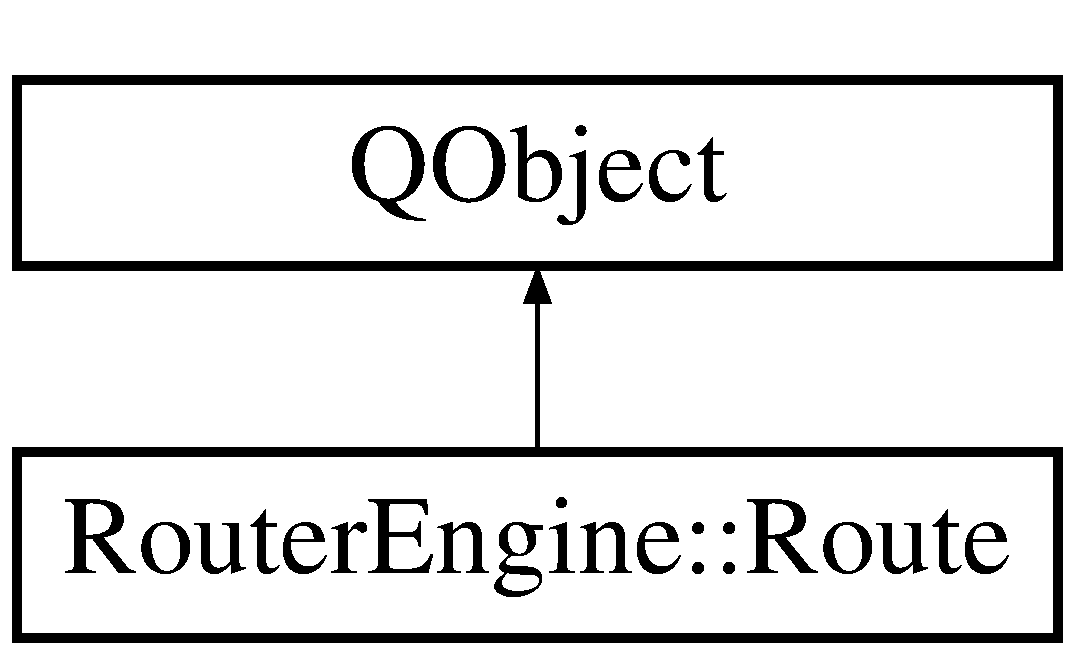
\includegraphics[height=2.000000cm]{classRouterEngine_1_1Route}
\end{center}
\end{figure}
\subsection*{Signals}
\begin{DoxyCompactItemize}
\item 
\mbox{\Hypertarget{classRouterEngine_1_1Route_a25ecf4bea955cc54810e48ed72b47146}\label{classRouterEngine_1_1Route_a25ecf4bea955cc54810e48ed72b47146}} 
void {\bfseries legs\+Changed} ()
\item 
\mbox{\Hypertarget{classRouterEngine_1_1Route_a5f23c83b0200aec7369ab1beff6edb21}\label{classRouterEngine_1_1Route_a5f23c83b0200aec7369ab1beff6edb21}} 
void {\bfseries transfers\+Changed} ()
\item 
\mbox{\Hypertarget{classRouterEngine_1_1Route_a4dd9643a1f7991afdcb167296d9f2fac}\label{classRouterEngine_1_1Route_a4dd9643a1f7991afdcb167296d9f2fac}} 
void {\bfseries trip\+Alerts\+Changed} ()
\item 
\mbox{\Hypertarget{classRouterEngine_1_1Route_a1ea5875ee80dca0f253caee323f23410}\label{classRouterEngine_1_1Route_a1ea5875ee80dca0f253caee323f23410}} 
void {\bfseries vehicle\+Alerts\+Changed} ()
\item 
\mbox{\Hypertarget{classRouterEngine_1_1Route_a42ba6dd381b51f8c9fb31bfd18386674}\label{classRouterEngine_1_1Route_a42ba6dd381b51f8c9fb31bfd18386674}} 
void {\bfseries remarks\+Changed} ()
\end{DoxyCompactItemize}
\subsection*{Public Member Functions}
\begin{DoxyCompactItemize}
\item 
\mbox{\Hypertarget{classRouterEngine_1_1Route_af55797a1f0895e2c361aa48c7b17a83c}\label{classRouterEngine_1_1Route_af55797a1f0895e2c361aa48c7b17a83c}} 
{\bfseries Route} (const Q\+List$<$ \mbox{\hyperlink{classRouterEngine_1_1RouteLeg}{Router\+Engine\+::\+Route\+Leg}} $\ast$$>$ \&legs, const Q\+List$<$ \mbox{\hyperlink{classRouterEngine_1_1Transfer}{Router\+Engine\+::\+Transfer}} $\ast$$>$ \&transfers, const Q\+List$<$ \mbox{\hyperlink{classAlertsEngine_1_1Message}{Alerts\+Engine\+::\+Message}} $\ast$$>$ \&trip\+Alerts, const Q\+List$<$ \mbox{\hyperlink{classAlertsEngine_1_1Message}{Alerts\+Engine\+::\+Message}} $\ast$$>$ \&vehicle\+Alerts, const Q\+List$<$ \mbox{\hyperlink{classAlertsEngine_1_1Message}{Alerts\+Engine\+::\+Message}} $\ast$$>$ \&remarks, Q\+Object $\ast$parent=nullptr)
\item 
\mbox{\Hypertarget{classRouterEngine_1_1Route_a4b2d697502c5de4298cb8f6cfc14e22c}\label{classRouterEngine_1_1Route_a4b2d697502c5de4298cb8f6cfc14e22c}} 
{\bfseries Route} (const Q\+List$<$ \mbox{\hyperlink{classRouterEngine_1_1RouteLeg}{Route\+Leg}} $\ast$$>$ \&legs, Q\+Object $\ast$parent=nullptr)
\item 
\mbox{\Hypertarget{classRouterEngine_1_1Route_a552677b912038bcaea9f2bf877cf05ce}\label{classRouterEngine_1_1Route_a552677b912038bcaea9f2bf877cf05ce}} 
Q\+List$<$ \mbox{\hyperlink{classRouterEngine_1_1RouteLeg}{Router\+Engine\+::\+Route\+Leg}} $\ast$ $>$ {\bfseries legs} () const
\item 
\mbox{\Hypertarget{classRouterEngine_1_1Route_ad51ae14971b6ce3ef88d79d088327b24}\label{classRouterEngine_1_1Route_ad51ae14971b6ce3ef88d79d088327b24}} 
void {\bfseries set\+Legs} (const Q\+List$<$ \mbox{\hyperlink{classRouterEngine_1_1RouteLeg}{Route\+Leg}} $\ast$$>$ \&legs)
\item 
\mbox{\Hypertarget{classRouterEngine_1_1Route_a1bdf547bd8b4d36c1fa7073b8a66e3a0}\label{classRouterEngine_1_1Route_a1bdf547bd8b4d36c1fa7073b8a66e3a0}} 
Q\+List$<$ \mbox{\hyperlink{classRouterEngine_1_1Transfer}{Router\+Engine\+::\+Transfer}} $\ast$ $>$ {\bfseries transfers} () const
\item 
\mbox{\Hypertarget{classRouterEngine_1_1Route_a26d4b164819441f1df27b0ef7c237e9c}\label{classRouterEngine_1_1Route_a26d4b164819441f1df27b0ef7c237e9c}} 
void {\bfseries set\+Transfers} (const Q\+List$<$ \mbox{\hyperlink{classRouterEngine_1_1Transfer}{Router\+Engine\+::\+Transfer}} $\ast$$>$ \&transfers)
\item 
\mbox{\Hypertarget{classRouterEngine_1_1Route_aa92be26a084deed2d391db6ca01fe3e9}\label{classRouterEngine_1_1Route_aa92be26a084deed2d391db6ca01fe3e9}} 
Q\+List$<$ \mbox{\hyperlink{classAlertsEngine_1_1Message}{Alerts\+Engine\+::\+Message}} $\ast$ $>$ {\bfseries trip\+Alerts} () const
\item 
\mbox{\Hypertarget{classRouterEngine_1_1Route_a546761b42b316b6e7ca2b8294fa06f79}\label{classRouterEngine_1_1Route_a546761b42b316b6e7ca2b8294fa06f79}} 
void {\bfseries set\+Trip\+Alerts} (const Q\+List$<$ \mbox{\hyperlink{classAlertsEngine_1_1Message}{Alerts\+Engine\+::\+Message}} $\ast$$>$ \&trip\+Alerts)
\item 
\mbox{\Hypertarget{classRouterEngine_1_1Route_a2d3c6fd345bd099e769ad06896199bc6}\label{classRouterEngine_1_1Route_a2d3c6fd345bd099e769ad06896199bc6}} 
Q\+List$<$ \mbox{\hyperlink{classAlertsEngine_1_1Message}{Alerts\+Engine\+::\+Message}} $\ast$ $>$ {\bfseries vehicle\+Alerts} () const
\item 
\mbox{\Hypertarget{classRouterEngine_1_1Route_a9f8e7a91afcd6e84cdca7870d7d6d8e4}\label{classRouterEngine_1_1Route_a9f8e7a91afcd6e84cdca7870d7d6d8e4}} 
void {\bfseries set\+Vehicle\+Alerts} (const Q\+List$<$ \mbox{\hyperlink{classAlertsEngine_1_1Message}{Alerts\+Engine\+::\+Message}} $\ast$$>$ \&vehicle\+Alerts)
\item 
\mbox{\Hypertarget{classRouterEngine_1_1Route_a003a75085fca704ade0509ccc09ce0e6}\label{classRouterEngine_1_1Route_a003a75085fca704ade0509ccc09ce0e6}} 
Q\+List$<$ \mbox{\hyperlink{classAlertsEngine_1_1Message}{Alerts\+Engine\+::\+Message}} $\ast$ $>$ {\bfseries remarks} () const
\item 
\mbox{\Hypertarget{classRouterEngine_1_1Route_ad007e0843cf6315fbbd3a2e3ec0bedce}\label{classRouterEngine_1_1Route_ad007e0843cf6315fbbd3a2e3ec0bedce}} 
void {\bfseries set\+Remarks} (const Q\+List$<$ \mbox{\hyperlink{classAlertsEngine_1_1Message}{Alerts\+Engine\+::\+Message}} $\ast$$>$ \&remarks)
\item 
\mbox{\Hypertarget{classRouterEngine_1_1Route_ad5b5241574cdf253e388c32e48e8f76c}\label{classRouterEngine_1_1Route_ad5b5241574cdf253e388c32e48e8f76c}} 
qint64 {\bfseries duration} () const
\item 
\mbox{\Hypertarget{classRouterEngine_1_1Route_a9d863b61b3ae63d327f0f6b39c50f2e6}\label{classRouterEngine_1_1Route_a9d863b61b3ae63d327f0f6b39c50f2e6}} 
qint64 {\bfseries duration\+With\+Delays} () const
\item 
\mbox{\Hypertarget{classRouterEngine_1_1Route_a50cf1f2f69b7f7a2f8b80e335f69789f}\label{classRouterEngine_1_1Route_a50cf1f2f69b7f7a2f8b80e335f69789f}} 
Q\+Date\+Time {\bfseries departure\+Time} () const
\item 
\mbox{\Hypertarget{classRouterEngine_1_1Route_a0faef1fc72bc4e1975d7036bc07aa6aa}\label{classRouterEngine_1_1Route_a0faef1fc72bc4e1975d7036bc07aa6aa}} 
qint16 {\bfseries departure\+Delay} () const
\item 
\mbox{\Hypertarget{classRouterEngine_1_1Route_a3eb15593ee1a363754828d0254cc4630}\label{classRouterEngine_1_1Route_a3eb15593ee1a363754828d0254cc4630}} 
Q\+Date\+Time {\bfseries arrival\+Time} () const
\item 
\mbox{\Hypertarget{classRouterEngine_1_1Route_a353a840fae9c1a1e4643a75f523ea969}\label{classRouterEngine_1_1Route_a353a840fae9c1a1e4643a75f523ea969}} 
qint16 {\bfseries arrival\+Delay} () const
\item 
\mbox{\Hypertarget{classRouterEngine_1_1Route_abd2ebc855744a545250f40ea959f585e}\label{classRouterEngine_1_1Route_abd2ebc855744a545250f40ea959f585e}} 
qint16 {\bfseries transfer\+Count} () const
\item 
\mbox{\Hypertarget{classRouterEngine_1_1Route_accb0f33bbb00a81500b545368cbe19c8}\label{classRouterEngine_1_1Route_accb0f33bbb00a81500b545368cbe19c8}} 
qint16 {\bfseries station\+Count} () const
\item 
\mbox{\Hypertarget{classRouterEngine_1_1Route_a9f4cdb95f949fc8607382cf7760d908c}\label{classRouterEngine_1_1Route_a9f4cdb95f949fc8607382cf7760d908c}} 
Q\+String {\bfseries departure\+Platform} () const
\item 
\mbox{\Hypertarget{classRouterEngine_1_1Route_a28bc0b5a2c1571e24b97e8826ae3e904}\label{classRouterEngine_1_1Route_a28bc0b5a2c1571e24b97e8826ae3e904}} 
bool {\bfseries is\+Departure\+Platform\+Normal} () const
\item 
\mbox{\Hypertarget{classRouterEngine_1_1Route_a504fbafeda1f8a5ef3466eb511ff3611}\label{classRouterEngine_1_1Route_a504fbafeda1f8a5ef3466eb511ff3611}} 
Q\+String {\bfseries arrival\+Platform} () const
\item 
\mbox{\Hypertarget{classRouterEngine_1_1Route_a7ce1a7f317253de637c9e13463a49940}\label{classRouterEngine_1_1Route_a7ce1a7f317253de637c9e13463a49940}} 
bool {\bfseries is\+Arrival\+Platform\+Normal} () const
\item 
\mbox{\Hypertarget{classRouterEngine_1_1Route_a360aac800ab7ff241a274c162fc634de}\label{classRouterEngine_1_1Route_a360aac800ab7ff241a274c162fc634de}} 
\mbox{\hyperlink{classRouterEngine_1_1Transfer}{Router\+Engine\+::\+Transfer}} $\ast$ {\bfseries departure\+Station} () const
\item 
\mbox{\Hypertarget{classRouterEngine_1_1Route_a7d8ed78f4287f2df45f14b0bbeb5ec23}\label{classRouterEngine_1_1Route_a7d8ed78f4287f2df45f14b0bbeb5ec23}} 
\mbox{\hyperlink{classRouterEngine_1_1Transfer}{Router\+Engine\+::\+Transfer}} $\ast$ {\bfseries arrival\+Station} () const
\item 
\mbox{\Hypertarget{classRouterEngine_1_1Route_a6d4bee0d56c75836510337d2d4e952bc}\label{classRouterEngine_1_1Route_a6d4bee0d56c75836510337d2d4e952bc}} 
bool {\bfseries is\+Partially\+Canceled} () const
\end{DoxyCompactItemize}
\subsection*{Private Attributes}
\begin{DoxyCompactItemize}
\item 
\mbox{\Hypertarget{classRouterEngine_1_1Route_aae1f4b3f94a5f3a9b4130a440cd38dfd}\label{classRouterEngine_1_1Route_aae1f4b3f94a5f3a9b4130a440cd38dfd}} 
Q\+List$<$ \mbox{\hyperlink{classRouterEngine_1_1RouteLeg}{Router\+Engine\+::\+Route\+Leg}} $\ast$ $>$ {\bfseries m\+\_\+legs}
\item 
\mbox{\Hypertarget{classRouterEngine_1_1Route_a44ca2440c72766809c21452cf4ec91c9}\label{classRouterEngine_1_1Route_a44ca2440c72766809c21452cf4ec91c9}} 
Q\+List$<$ \mbox{\hyperlink{classRouterEngine_1_1Transfer}{Router\+Engine\+::\+Transfer}} $\ast$ $>$ {\bfseries m\+\_\+transfers}
\item 
\mbox{\Hypertarget{classRouterEngine_1_1Route_a62219fa709ea150e5a92f75dd344b295}\label{classRouterEngine_1_1Route_a62219fa709ea150e5a92f75dd344b295}} 
Q\+List$<$ \mbox{\hyperlink{classAlertsEngine_1_1Message}{Alerts\+Engine\+::\+Message}} $\ast$ $>$ {\bfseries m\+\_\+trip\+Alerts}
\item 
\mbox{\Hypertarget{classRouterEngine_1_1Route_a78c36b4967b80623b424d5e4a9c77d9b}\label{classRouterEngine_1_1Route_a78c36b4967b80623b424d5e4a9c77d9b}} 
Q\+List$<$ \mbox{\hyperlink{classAlertsEngine_1_1Message}{Alerts\+Engine\+::\+Message}} $\ast$ $>$ {\bfseries m\+\_\+vehicle\+Alerts}
\item 
\mbox{\Hypertarget{classRouterEngine_1_1Route_a13f053604f806a1094f015a396aaa416}\label{classRouterEngine_1_1Route_a13f053604f806a1094f015a396aaa416}} 
Q\+List$<$ \mbox{\hyperlink{classAlertsEngine_1_1Message}{Alerts\+Engine\+::\+Message}} $\ast$ $>$ {\bfseries m\+\_\+remarks}
\end{DoxyCompactItemize}


The documentation for this class was generated from the following files\+:\begin{DoxyCompactItemize}
\item 
src/include/engines/router/routerroute.\+h\item 
src/engines/router/\mbox{\hyperlink{routerroute_8cpp}{routerroute.\+cpp}}\end{DoxyCompactItemize}

\hypertarget{classRouterEngine_1_1RouteLeg}{}\section{Router\+Engine\+:\+:Route\+Leg Class Reference}
\label{classRouterEngine_1_1RouteLeg}\index{Router\+Engine\+::\+Route\+Leg@{Router\+Engine\+::\+Route\+Leg}}
Inheritance diagram for Router\+Engine\+:\+:Route\+Leg\+:\begin{figure}[H]
\begin{center}
\leavevmode
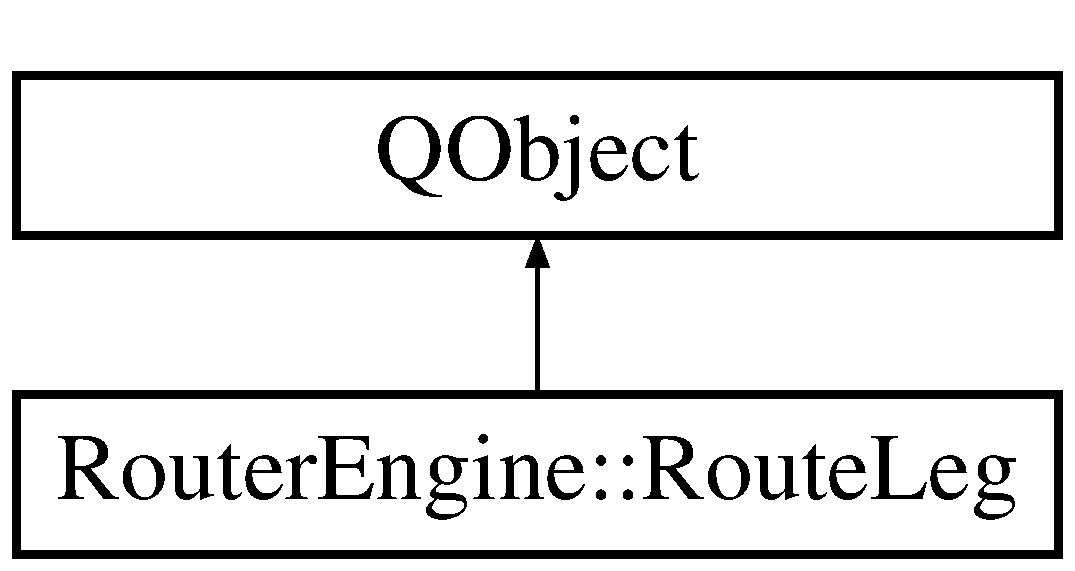
\includegraphics[height=2.000000cm]{classRouterEngine_1_1RouteLeg}
\end{center}
\end{figure}
\subsection*{Public Types}
\begin{DoxyCompactItemize}
\item 
\mbox{\Hypertarget{classRouterEngine_1_1RouteLeg_acdcc25212c113c641ee3fbaebb52a7bd}\label{classRouterEngine_1_1RouteLeg_acdcc25212c113c641ee3fbaebb52a7bd}} 
enum {\bfseries Type} \{ \newline
{\bfseries W\+A\+L\+K\+I\+NG}, 
{\bfseries B\+I\+C\+Y\+C\+LE}, 
{\bfseries B\+US}, 
{\bfseries T\+R\+AM}, 
\newline
{\bfseries M\+E\+T\+RO}, 
{\bfseries B\+O\+AT}, 
{\bfseries T\+A\+XI}, 
{\bfseries T\+R\+A\+IN}
 \}
\end{DoxyCompactItemize}
\subsection*{Signals}
\begin{DoxyCompactItemize}
\item 
\mbox{\Hypertarget{classRouterEngine_1_1RouteLeg_afbed2dc6199e75b1ac36111465f6f3d4}\label{classRouterEngine_1_1RouteLeg_afbed2dc6199e75b1ac36111465f6f3d4}} 
void {\bfseries type\+Changed} ()
\item 
\mbox{\Hypertarget{classRouterEngine_1_1RouteLeg_a11952e3a2fee4fa1d9f4fb56e69f0507}\label{classRouterEngine_1_1RouteLeg_a11952e3a2fee4fa1d9f4fb56e69f0507}} 
void {\bfseries vehicle\+Information\+Changed} ()
\item 
\mbox{\Hypertarget{classRouterEngine_1_1RouteLeg_a1d28c018a24f8eed64064d685a1f6a09}\label{classRouterEngine_1_1RouteLeg_a1d28c018a24f8eed64064d685a1f6a09}} 
void {\bfseries stops\+Changed} ()
\item 
\mbox{\Hypertarget{classRouterEngine_1_1RouteLeg_a8422dd38411600b6ffc2aa490633115b}\label{classRouterEngine_1_1RouteLeg_a8422dd38411600b6ffc2aa490633115b}} 
void {\bfseries departure\+Changed} ()
\item 
\mbox{\Hypertarget{classRouterEngine_1_1RouteLeg_abc2b662f878119adb9ded14f3d1fd5f9}\label{classRouterEngine_1_1RouteLeg_abc2b662f878119adb9ded14f3d1fd5f9}} 
void {\bfseries arrival\+Changed} ()
\item 
\mbox{\Hypertarget{classRouterEngine_1_1RouteLeg_a670f844ac7c005ae2dd3a18b42bff29a}\label{classRouterEngine_1_1RouteLeg_a670f844ac7c005ae2dd3a18b42bff29a}} 
void {\bfseries station\+Changed} ()
\end{DoxyCompactItemize}
\subsection*{Public Member Functions}
\begin{DoxyCompactItemize}
\item 
\mbox{\Hypertarget{classRouterEngine_1_1RouteLeg_a1c2b7ecc87cab7b5a4ff69d07f4e646a}\label{classRouterEngine_1_1RouteLeg_a1c2b7ecc87cab7b5a4ff69d07f4e646a}} 
{\bfseries Route\+Leg} (const Router\+Engine\+::\+Route\+Leg\+::\+Type \&type, \mbox{\hyperlink{classVehicleEngine_1_1Vehicle}{Vehicle\+Engine\+::\+Vehicle}} $\ast$vehicle\+Information, \mbox{\hyperlink{classRouterEngine_1_1RouteLegEnd}{Router\+Engine\+::\+Route\+Leg\+End}} $\ast$departure, \mbox{\hyperlink{classRouterEngine_1_1RouteLegEnd}{Router\+Engine\+::\+Route\+Leg\+End}} $\ast$arrival, Q\+Object $\ast$parent=nullptr)
\item 
\mbox{\Hypertarget{classRouterEngine_1_1RouteLeg_a30acf2e2a57217cd2f588475ea3c6e80}\label{classRouterEngine_1_1RouteLeg_a30acf2e2a57217cd2f588475ea3c6e80}} 
Router\+Engine\+::\+Route\+Leg\+::\+Type {\bfseries type} () const
\item 
\mbox{\Hypertarget{classRouterEngine_1_1RouteLeg_ada52c9281e1b545753e0beeded6f8e4a}\label{classRouterEngine_1_1RouteLeg_ada52c9281e1b545753e0beeded6f8e4a}} 
void {\bfseries set\+Type} (const Router\+Engine\+::\+Route\+Leg\+::\+Type \&type)
\item 
\mbox{\Hypertarget{classRouterEngine_1_1RouteLeg_a086d61b828cd572797ec327710eb4088}\label{classRouterEngine_1_1RouteLeg_a086d61b828cd572797ec327710eb4088}} 
\mbox{\hyperlink{classVehicleEngine_1_1Vehicle}{Vehicle\+Engine\+::\+Vehicle}} $\ast$ {\bfseries vehicle\+Information} () const
\item 
\mbox{\Hypertarget{classRouterEngine_1_1RouteLeg_a535891ef84cac1a875b3f1a58404c227}\label{classRouterEngine_1_1RouteLeg_a535891ef84cac1a875b3f1a58404c227}} 
void {\bfseries set\+Vehicle\+Information} (\mbox{\hyperlink{classVehicleEngine_1_1Vehicle}{Vehicle\+Engine\+::\+Vehicle}} $\ast$vehicle\+Information)
\item 
\mbox{\Hypertarget{classRouterEngine_1_1RouteLeg_a77dd1b04134b55cbc6dc031f5e6d6379}\label{classRouterEngine_1_1RouteLeg_a77dd1b04134b55cbc6dc031f5e6d6379}} 
\mbox{\hyperlink{classRouterEngine_1_1RouteLegEnd}{Router\+Engine\+::\+Route\+Leg\+End}} $\ast$ {\bfseries departure} () const
\item 
\mbox{\Hypertarget{classRouterEngine_1_1RouteLeg_a80f8a85b74c662e1832313677a5bc7f3}\label{classRouterEngine_1_1RouteLeg_a80f8a85b74c662e1832313677a5bc7f3}} 
void {\bfseries set\+Departure} (\mbox{\hyperlink{classRouterEngine_1_1RouteLegEnd}{Router\+Engine\+::\+Route\+Leg\+End}} $\ast$departure)
\item 
\mbox{\Hypertarget{classRouterEngine_1_1RouteLeg_a82998f111cb81b20e043e45e1e8c0ebc}\label{classRouterEngine_1_1RouteLeg_a82998f111cb81b20e043e45e1e8c0ebc}} 
\mbox{\hyperlink{classRouterEngine_1_1RouteLegEnd}{Router\+Engine\+::\+Route\+Leg\+End}} $\ast$ {\bfseries arrival} () const
\item 
\mbox{\Hypertarget{classRouterEngine_1_1RouteLeg_aca6d3ade15e711e0bfe963b58de7a20f}\label{classRouterEngine_1_1RouteLeg_aca6d3ade15e711e0bfe963b58de7a20f}} 
void {\bfseries set\+Arrival} (\mbox{\hyperlink{classRouterEngine_1_1RouteLegEnd}{Router\+Engine\+::\+Route\+Leg\+End}} $\ast$arrival)
\item 
\mbox{\Hypertarget{classRouterEngine_1_1RouteLeg_a5643c5924f06246dd7e3ae9b07b70bca}\label{classRouterEngine_1_1RouteLeg_a5643c5924f06246dd7e3ae9b07b70bca}} 
\mbox{\hyperlink{classStationEngine_1_1Station}{Station\+Engine\+::\+Station}} $\ast$ {\bfseries station} () const
\end{DoxyCompactItemize}
\subsection*{Private Attributes}
\begin{DoxyCompactItemize}
\item 
\mbox{\Hypertarget{classRouterEngine_1_1RouteLeg_abefba3e1870352470f547966736261d0}\label{classRouterEngine_1_1RouteLeg_abefba3e1870352470f547966736261d0}} 
Router\+Engine\+::\+Route\+Leg\+::\+Type {\bfseries m\+\_\+type}
\item 
\mbox{\Hypertarget{classRouterEngine_1_1RouteLeg_a602cdb13e3929a0378506661ed7336a7}\label{classRouterEngine_1_1RouteLeg_a602cdb13e3929a0378506661ed7336a7}} 
\mbox{\hyperlink{classVehicleEngine_1_1Vehicle}{Vehicle\+Engine\+::\+Vehicle}} $\ast$ {\bfseries m\+\_\+vehicle\+Information}
\item 
\mbox{\Hypertarget{classRouterEngine_1_1RouteLeg_a3a3354a3f654f5c923339a30beba7339}\label{classRouterEngine_1_1RouteLeg_a3a3354a3f654f5c923339a30beba7339}} 
\mbox{\hyperlink{classRouterEngine_1_1RouteLegEnd}{Router\+Engine\+::\+Route\+Leg\+End}} $\ast$ {\bfseries m\+\_\+departure}
\item 
\mbox{\Hypertarget{classRouterEngine_1_1RouteLeg_a85b14ef10073dec49d7fa2e20e35e54e}\label{classRouterEngine_1_1RouteLeg_a85b14ef10073dec49d7fa2e20e35e54e}} 
\mbox{\hyperlink{classRouterEngine_1_1RouteLegEnd}{Router\+Engine\+::\+Route\+Leg\+End}} $\ast$ {\bfseries m\+\_\+arrival}
\end{DoxyCompactItemize}


The documentation for this class was generated from the following files\+:\begin{DoxyCompactItemize}
\item 
src/include/engines/router/routerrouteleg.\+h\item 
src/engines/router/\mbox{\hyperlink{routerrouteleg_8cpp}{routerrouteleg.\+cpp}}\end{DoxyCompactItemize}

\hypertarget{classRouterEngine_1_1RouteLegEnd}{}\section{Router\+Engine\+:\+:Route\+Leg\+End Class Reference}
\label{classRouterEngine_1_1RouteLegEnd}\index{Router\+Engine\+::\+Route\+Leg\+End@{Router\+Engine\+::\+Route\+Leg\+End}}
Inheritance diagram for Router\+Engine\+:\+:Route\+Leg\+End\+:\begin{figure}[H]
\begin{center}
\leavevmode
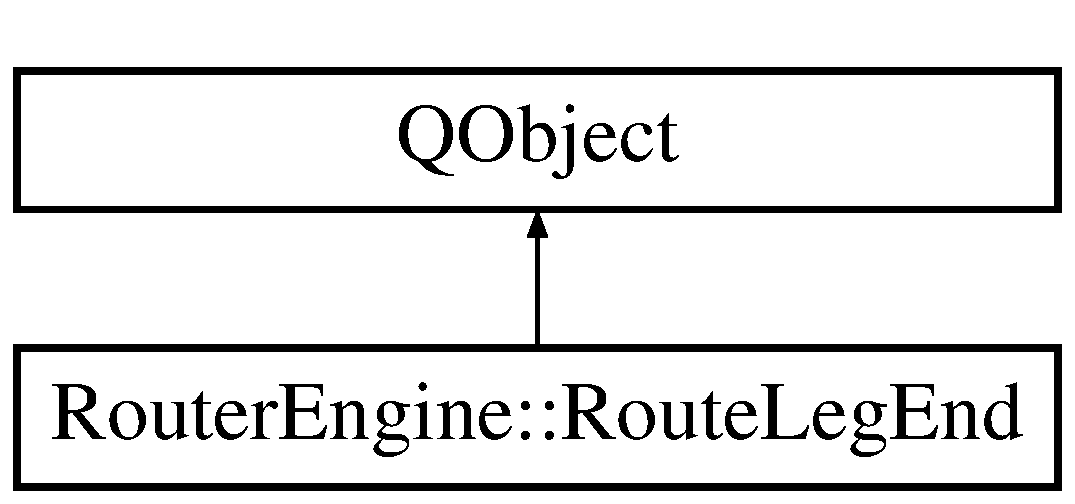
\includegraphics[height=2.000000cm]{classRouterEngine_1_1RouteLegEnd}
\end{center}
\end{figure}
\subsection*{Signals}
\begin{DoxyCompactItemize}
\item 
\mbox{\Hypertarget{classRouterEngine_1_1RouteLegEnd_a7c2f6e278e8c36277cd7375d404f9da7}\label{classRouterEngine_1_1RouteLegEnd_a7c2f6e278e8c36277cd7375d404f9da7}} 
void {\bfseries uri\+Changed} ()
\item 
\mbox{\Hypertarget{classRouterEngine_1_1RouteLegEnd_add70393bdb51cd803515054a865cb4cc}\label{classRouterEngine_1_1RouteLegEnd_add70393bdb51cd803515054a865cb4cc}} 
void {\bfseries time\+Changed} ()
\item 
\mbox{\Hypertarget{classRouterEngine_1_1RouteLegEnd_acd19ab71a7074629246ba2fa21e74b1b}\label{classRouterEngine_1_1RouteLegEnd_acd19ab71a7074629246ba2fa21e74b1b}} 
void {\bfseries station\+Changed} ()
\item 
\mbox{\Hypertarget{classRouterEngine_1_1RouteLegEnd_a5ebc7a99f6c9feb9e7a4f8200b85af64}\label{classRouterEngine_1_1RouteLegEnd_a5ebc7a99f6c9feb9e7a4f8200b85af64}} 
void {\bfseries platform\+Changed} ()
\item 
\mbox{\Hypertarget{classRouterEngine_1_1RouteLegEnd_a7ec769dededbb588e5d389df9d5492fa}\label{classRouterEngine_1_1RouteLegEnd_a7ec769dededbb588e5d389df9d5492fa}} 
void {\bfseries is\+Normal\+Platform\+Changed} ()
\item 
\mbox{\Hypertarget{classRouterEngine_1_1RouteLegEnd_aa8d92db59e92c6925c4d380a3bbd4d7a}\label{classRouterEngine_1_1RouteLegEnd_aa8d92db59e92c6925c4d380a3bbd4d7a}} 
void {\bfseries delay\+Changed} ()
\item 
\mbox{\Hypertarget{classRouterEngine_1_1RouteLegEnd_a885f3487bcd25266619ee6f803190c68}\label{classRouterEngine_1_1RouteLegEnd_a885f3487bcd25266619ee6f803190c68}} 
void {\bfseries is\+Canceled\+Changed} ()
\item 
\mbox{\Hypertarget{classRouterEngine_1_1RouteLegEnd_a8d4b0ade9234f22a423a0b4b3f3153f9}\label{classRouterEngine_1_1RouteLegEnd_a8d4b0ade9234f22a423a0b4b3f3153f9}} 
void {\bfseries is\+Passed\+Changed} ()
\item 
\mbox{\Hypertarget{classRouterEngine_1_1RouteLegEnd_a9be6e797f6c63cb45e258df5b43f1ceb}\label{classRouterEngine_1_1RouteLegEnd_a9be6e797f6c63cb45e258df5b43f1ceb}} 
void {\bfseries occupancy\+Level\+Changed} ()
\end{DoxyCompactItemize}
\subsection*{Public Member Functions}
\begin{DoxyCompactItemize}
\item 
\mbox{\Hypertarget{classRouterEngine_1_1RouteLegEnd_ac8d5c3ffe9d65a83cae8c7de5962e818}\label{classRouterEngine_1_1RouteLegEnd_ac8d5c3ffe9d65a83cae8c7de5962e818}} 
{\bfseries Route\+Leg\+End} (const Q\+Url \&uri, const Q\+Date\+Time \&time, \mbox{\hyperlink{classStationEngine_1_1Station}{Station\+Engine\+::\+Station}} $\ast$station, const Q\+String \&platform, const bool \&is\+Normal\+Platform, const qint16 \&delay, const bool \&is\+Canceled, const bool \&is\+Passed, const Vehicle\+Engine\+::\+Stop\+::\+Occupancy\+Level \&occupancy\+Level, Q\+Object $\ast$parent=nullptr)
\item 
\mbox{\Hypertarget{classRouterEngine_1_1RouteLegEnd_a5a6b2f91b5503c7dfb410e1e426ed721}\label{classRouterEngine_1_1RouteLegEnd_a5a6b2f91b5503c7dfb410e1e426ed721}} 
Q\+Url {\bfseries uri} () const
\item 
\mbox{\Hypertarget{classRouterEngine_1_1RouteLegEnd_aaa056987791da9ae776100926dd8141f}\label{classRouterEngine_1_1RouteLegEnd_aaa056987791da9ae776100926dd8141f}} 
void {\bfseries set\+Uri} (const Q\+Url \&uri)
\item 
\mbox{\Hypertarget{classRouterEngine_1_1RouteLegEnd_aa3050fc8b747490c3c06f7e451e9dba1}\label{classRouterEngine_1_1RouteLegEnd_aa3050fc8b747490c3c06f7e451e9dba1}} 
Q\+Date\+Time {\bfseries time} () const
\item 
\mbox{\Hypertarget{classRouterEngine_1_1RouteLegEnd_ae56d26ce44fa8261ca43834cbdd79a7d}\label{classRouterEngine_1_1RouteLegEnd_ae56d26ce44fa8261ca43834cbdd79a7d}} 
void {\bfseries set\+Time} (const Q\+Date\+Time \&time)
\item 
\mbox{\Hypertarget{classRouterEngine_1_1RouteLegEnd_ac79a006d8c9d4cbcd97567beec83784a}\label{classRouterEngine_1_1RouteLegEnd_ac79a006d8c9d4cbcd97567beec83784a}} 
\mbox{\hyperlink{classStationEngine_1_1Station}{Station\+Engine\+::\+Station}} $\ast$ {\bfseries station} () const
\item 
\mbox{\Hypertarget{classRouterEngine_1_1RouteLegEnd_a49fb362e35a88711cc794c95d8c94c4e}\label{classRouterEngine_1_1RouteLegEnd_a49fb362e35a88711cc794c95d8c94c4e}} 
void {\bfseries set\+Station} (\mbox{\hyperlink{classStationEngine_1_1Station}{Station\+Engine\+::\+Station}} $\ast$station)
\item 
\mbox{\Hypertarget{classRouterEngine_1_1RouteLegEnd_a5cd38e1cde6c5632b60a183226825732}\label{classRouterEngine_1_1RouteLegEnd_a5cd38e1cde6c5632b60a183226825732}} 
Q\+String {\bfseries platform} () const
\item 
\mbox{\Hypertarget{classRouterEngine_1_1RouteLegEnd_ab44931f5c47e9497355d47ba44b896e5}\label{classRouterEngine_1_1RouteLegEnd_ab44931f5c47e9497355d47ba44b896e5}} 
void {\bfseries set\+Platform} (const Q\+String \&platform)
\item 
\mbox{\Hypertarget{classRouterEngine_1_1RouteLegEnd_a24879496826d9e513cf6ffb393237db8}\label{classRouterEngine_1_1RouteLegEnd_a24879496826d9e513cf6ffb393237db8}} 
bool {\bfseries is\+Normal\+Platform} () const
\item 
\mbox{\Hypertarget{classRouterEngine_1_1RouteLegEnd_acfa2dac12a3e1e3f7a8bab5e9f55482b}\label{classRouterEngine_1_1RouteLegEnd_acfa2dac12a3e1e3f7a8bab5e9f55482b}} 
void {\bfseries set\+Is\+Normal\+Platform} (bool is\+Normal\+Platform)
\item 
\mbox{\Hypertarget{classRouterEngine_1_1RouteLegEnd_ae8c0b35f77c5a66d5d5afa96f7eb4625}\label{classRouterEngine_1_1RouteLegEnd_ae8c0b35f77c5a66d5d5afa96f7eb4625}} 
qint16 {\bfseries delay} () const
\item 
\mbox{\Hypertarget{classRouterEngine_1_1RouteLegEnd_a693365fb2083839ddd5ebf17d5032121}\label{classRouterEngine_1_1RouteLegEnd_a693365fb2083839ddd5ebf17d5032121}} 
void {\bfseries set\+Delay} (const qint16 \&delay)
\item 
\mbox{\Hypertarget{classRouterEngine_1_1RouteLegEnd_afb87a99a388b7dd36c5357f57aeb361b}\label{classRouterEngine_1_1RouteLegEnd_afb87a99a388b7dd36c5357f57aeb361b}} 
bool {\bfseries is\+Canceled} () const
\item 
\mbox{\Hypertarget{classRouterEngine_1_1RouteLegEnd_ace382e058479c3ec424d8321df838667}\label{classRouterEngine_1_1RouteLegEnd_ace382e058479c3ec424d8321df838667}} 
void {\bfseries set\+Is\+Canceled} (bool is\+Canceled)
\item 
\mbox{\Hypertarget{classRouterEngine_1_1RouteLegEnd_afb7a50823d8529b913832bd358bf4983}\label{classRouterEngine_1_1RouteLegEnd_afb7a50823d8529b913832bd358bf4983}} 
bool {\bfseries is\+Passed} () const
\item 
\mbox{\Hypertarget{classRouterEngine_1_1RouteLegEnd_af96b512dc585624f8d9bbaed165dafb8}\label{classRouterEngine_1_1RouteLegEnd_af96b512dc585624f8d9bbaed165dafb8}} 
void {\bfseries set\+Is\+Passed} (bool is\+Passed)
\item 
\mbox{\Hypertarget{classRouterEngine_1_1RouteLegEnd_ad5ddf5854bee2bf268728707b405ae4c}\label{classRouterEngine_1_1RouteLegEnd_ad5ddf5854bee2bf268728707b405ae4c}} 
Vehicle\+Engine\+::\+Stop\+::\+Occupancy\+Level {\bfseries occupancy\+Level} () const
\item 
\mbox{\Hypertarget{classRouterEngine_1_1RouteLegEnd_ad71a1a0c0d96125eb1833bc63cd4abbf}\label{classRouterEngine_1_1RouteLegEnd_ad71a1a0c0d96125eb1833bc63cd4abbf}} 
void {\bfseries set\+Occupancy\+Level} (const Vehicle\+Engine\+::\+Stop\+::\+Occupancy\+Level \&occupancy\+Level)
\end{DoxyCompactItemize}
\subsection*{Private Attributes}
\begin{DoxyCompactItemize}
\item 
\mbox{\Hypertarget{classRouterEngine_1_1RouteLegEnd_ad3d85af3fde972892bdd47239a402bd5}\label{classRouterEngine_1_1RouteLegEnd_ad3d85af3fde972892bdd47239a402bd5}} 
Q\+Url {\bfseries m\+\_\+uri}
\item 
\mbox{\Hypertarget{classRouterEngine_1_1RouteLegEnd_a63593b8c83639b2afad706a12bfeafa1}\label{classRouterEngine_1_1RouteLegEnd_a63593b8c83639b2afad706a12bfeafa1}} 
Q\+Date\+Time {\bfseries m\+\_\+time}
\item 
\mbox{\Hypertarget{classRouterEngine_1_1RouteLegEnd_ad8d8b12f9ea85211e3cf61939f9c3757}\label{classRouterEngine_1_1RouteLegEnd_ad8d8b12f9ea85211e3cf61939f9c3757}} 
\mbox{\hyperlink{classStationEngine_1_1Station}{Station\+Engine\+::\+Station}} $\ast$ {\bfseries m\+\_\+station}
\item 
\mbox{\Hypertarget{classRouterEngine_1_1RouteLegEnd_a2365b77544223ce133f77a9b5d64435c}\label{classRouterEngine_1_1RouteLegEnd_a2365b77544223ce133f77a9b5d64435c}} 
Q\+String {\bfseries m\+\_\+platform}
\item 
\mbox{\Hypertarget{classRouterEngine_1_1RouteLegEnd_a229d67e5fc1a6085f445d6413a7a6079}\label{classRouterEngine_1_1RouteLegEnd_a229d67e5fc1a6085f445d6413a7a6079}} 
bool {\bfseries m\+\_\+is\+Normal\+Platform}
\item 
\mbox{\Hypertarget{classRouterEngine_1_1RouteLegEnd_a91b8ffd54ecdc215cd4a1e7dfc2b4f96}\label{classRouterEngine_1_1RouteLegEnd_a91b8ffd54ecdc215cd4a1e7dfc2b4f96}} 
qint16 {\bfseries m\+\_\+delay}
\item 
\mbox{\Hypertarget{classRouterEngine_1_1RouteLegEnd_a33d2a432407bc94aa1dd3a6b5a062611}\label{classRouterEngine_1_1RouteLegEnd_a33d2a432407bc94aa1dd3a6b5a062611}} 
bool {\bfseries m\+\_\+is\+Canceled}
\item 
\mbox{\Hypertarget{classRouterEngine_1_1RouteLegEnd_a8c9e800864e99015e3e7a8f7ba2c8601}\label{classRouterEngine_1_1RouteLegEnd_a8c9e800864e99015e3e7a8f7ba2c8601}} 
bool {\bfseries m\+\_\+is\+Passed}
\item 
\mbox{\Hypertarget{classRouterEngine_1_1RouteLegEnd_ad4ebf526d4f94ae30418613e7eeb2b9d}\label{classRouterEngine_1_1RouteLegEnd_ad4ebf526d4f94ae30418613e7eeb2b9d}} 
Vehicle\+Engine\+::\+Stop\+::\+Occupancy\+Level {\bfseries m\+\_\+occupancy\+Level}
\end{DoxyCompactItemize}


The documentation for this class was generated from the following files\+:\begin{DoxyCompactItemize}
\item 
src/include/engines/router/routerroutelegend.\+h\item 
src/engines/router/\mbox{\hyperlink{routerroutelegend_8cpp}{routerroutelegend.\+cpp}}\end{DoxyCompactItemize}

\hypertarget{classStationEngine_1_1Station}{}\section{Station\+Engine\+:\+:Station Class Reference}
\label{classStationEngine_1_1Station}\index{Station\+Engine\+::\+Station@{Station\+Engine\+::\+Station}}
Inheritance diagram for Station\+Engine\+:\+:Station\+:\begin{figure}[H]
\begin{center}
\leavevmode
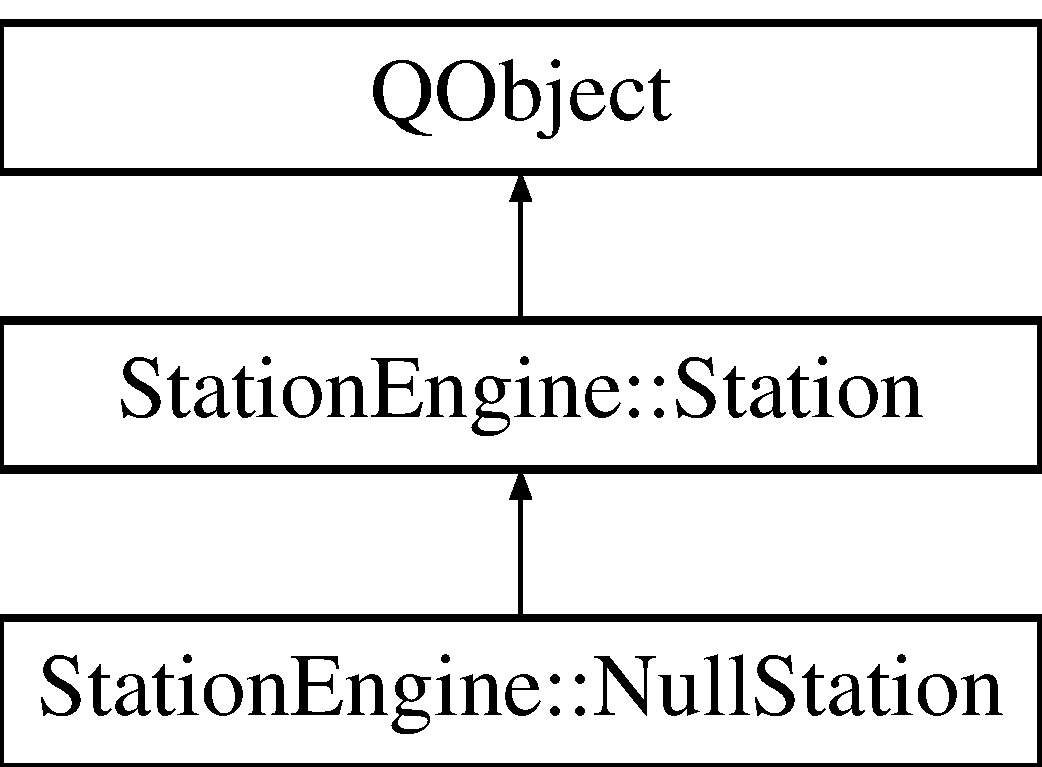
\includegraphics[height=3.000000cm]{classStationEngine_1_1Station}
\end{center}
\end{figure}
\subsection*{Public Types}
\begin{DoxyCompactItemize}
\item 
\mbox{\Hypertarget{classStationEngine_1_1Station_ac1bf5d8c9bbff48cb22a16ecb070e2ff}\label{classStationEngine_1_1Station_ac1bf5d8c9bbff48cb22a16ecb070e2ff}} 
enum {\bfseries Day} \{ \newline
{\bfseries M\+O\+N\+D\+AY}, 
{\bfseries T\+U\+E\+S\+D\+AY}, 
{\bfseries W\+E\+D\+N\+E\+S\+D\+AY}, 
{\bfseries T\+H\+U\+R\+S\+D\+AY}, 
\newline
{\bfseries F\+R\+I\+D\+AY}, 
{\bfseries S\+A\+T\+U\+R\+D\+AY}, 
{\bfseries S\+U\+N\+D\+AY}
 \}
\end{DoxyCompactItemize}
\subsection*{Signals}
\begin{DoxyCompactItemize}
\item 
\mbox{\Hypertarget{classStationEngine_1_1Station_a9768f01f112c58ebe3fdec8f7123bd7f}\label{classStationEngine_1_1Station_a9768f01f112c58ebe3fdec8f7123bd7f}} 
void {\bfseries uri\+Changed} ()
\item 
\mbox{\Hypertarget{classStationEngine_1_1Station_a61b7232a177c331c2b68634cf401fdce}\label{classStationEngine_1_1Station_a61b7232a177c331c2b68634cf401fdce}} 
void {\bfseries name\+Changed} ()
\item 
\mbox{\Hypertarget{classStationEngine_1_1Station_aaf68890e19657a56536af541f92036d2}\label{classStationEngine_1_1Station_aaf68890e19657a56536af541f92036d2}} 
void {\bfseries country\+Changed} ()
\item 
\mbox{\Hypertarget{classStationEngine_1_1Station_a5baf5f393c99bfecf52a65ad8913e901}\label{classStationEngine_1_1Station_a5baf5f393c99bfecf52a65ad8913e901}} 
void {\bfseries position\+Changed} ()
\item 
\mbox{\Hypertarget{classStationEngine_1_1Station_a5df6eee3f8c6c9a5d80605ade7eb1859}\label{classStationEngine_1_1Station_a5df6eee3f8c6c9a5d80605ade7eb1859}} 
void {\bfseries address\+Changed} ()
\item 
\mbox{\Hypertarget{classStationEngine_1_1Station_a0d096cd9af6f827a61301fc33ae67e33}\label{classStationEngine_1_1Station_a0d096cd9af6f827a61301fc33ae67e33}} 
void {\bfseries has\+Ticket\+Vending\+Machine\+Changed} ()
\item 
\mbox{\Hypertarget{classStationEngine_1_1Station_accf725debefd301f181e302b2d7929f9}\label{classStationEngine_1_1Station_accf725debefd301f181e302b2d7929f9}} 
void {\bfseries has\+Luggage\+Lockers\+Changed} ()
\item 
\mbox{\Hypertarget{classStationEngine_1_1Station_a4a31e8e1ce8ea6cb4cad9e968fe62933}\label{classStationEngine_1_1Station_a4a31e8e1ce8ea6cb4cad9e968fe62933}} 
void {\bfseries has\+Free\+Parking\+Changed} ()
\item 
\mbox{\Hypertarget{classStationEngine_1_1Station_acaf18dd75aa9d4b91778fae49ab70f3c}\label{classStationEngine_1_1Station_acaf18dd75aa9d4b91778fae49ab70f3c}} 
void {\bfseries has\+Taxi\+Changed} ()
\item 
\mbox{\Hypertarget{classStationEngine_1_1Station_ab9ccdadf3595ed110811dc89b1f978be}\label{classStationEngine_1_1Station_ab9ccdadf3595ed110811dc89b1f978be}} 
void {\bfseries has\+Bicylce\+Spots\+Changed} ()
\item 
\mbox{\Hypertarget{classStationEngine_1_1Station_a9195d51336bed5d0e8d3b53be4700d8b}\label{classStationEngine_1_1Station_a9195d51336bed5d0e8d3b53be4700d8b}} 
void {\bfseries has\+Blue\+Bike\+Changed} ()
\item 
\mbox{\Hypertarget{classStationEngine_1_1Station_a29614c5ef79f890a26c3e4f9193dbbbf}\label{classStationEngine_1_1Station_a29614c5ef79f890a26c3e4f9193dbbbf}} 
void {\bfseries has\+Bus\+Changed} ()
\item 
\mbox{\Hypertarget{classStationEngine_1_1Station_a0c50f6727a72e5a6b5dc024a9247d13d}\label{classStationEngine_1_1Station_a0c50f6727a72e5a6b5dc024a9247d13d}} 
void {\bfseries has\+Tram\+Changed} ()
\item 
\mbox{\Hypertarget{classStationEngine_1_1Station_ade4d9362d4f216810cb079f9bb4b6eeb}\label{classStationEngine_1_1Station_ade4d9362d4f216810cb079f9bb4b6eeb}} 
void {\bfseries has\+Metro\+Changed} ()
\item 
\mbox{\Hypertarget{classStationEngine_1_1Station_ae441a570b80a2ae4b341e224dd227e6f}\label{classStationEngine_1_1Station_ae441a570b80a2ae4b341e224dd227e6f}} 
void {\bfseries has\+Wheelchair\+Available\+Changed} ()
\item 
\mbox{\Hypertarget{classStationEngine_1_1Station_a4d75a1840b822b2a139486e95642cf88}\label{classStationEngine_1_1Station_a4d75a1840b822b2a139486e95642cf88}} 
void {\bfseries has\+Ramp\+Changed} ()
\item 
\mbox{\Hypertarget{classStationEngine_1_1Station_ab4f4bd762178514381f143fa18c17e95}\label{classStationEngine_1_1Station_ab4f4bd762178514381f143fa18c17e95}} 
void {\bfseries disabled\+Parking\+Spots\+Changed} ()
\item 
\mbox{\Hypertarget{classStationEngine_1_1Station_a05fea4dc58a6bbd128982cd6c57bb284}\label{classStationEngine_1_1Station_a05fea4dc58a6bbd128982cd6c57bb284}} 
void {\bfseries has\+Elevated\+Platform\+Changed} ()
\item 
\mbox{\Hypertarget{classStationEngine_1_1Station_a7209e0626829813742720a6d15f85cc3}\label{classStationEngine_1_1Station_a7209e0626829813742720a6d15f85cc3}} 
void {\bfseries has\+Escalator\+Up\+Changed} ()
\item 
\mbox{\Hypertarget{classStationEngine_1_1Station_aa3b3f3bce2829dbce79171dab951bd48}\label{classStationEngine_1_1Station_aa3b3f3bce2829dbce79171dab951bd48}} 
void {\bfseries has\+Escalator\+Down\+Changed} ()
\item 
\mbox{\Hypertarget{classStationEngine_1_1Station_a420f00930b1a9b96d28c2b285f6cd161}\label{classStationEngine_1_1Station_a420f00930b1a9b96d28c2b285f6cd161}} 
void {\bfseries has\+Hearing\+Aid\+Signal\+Changed} ()
\item 
\mbox{\Hypertarget{classStationEngine_1_1Station_a5859689456c15402abc729ba5c0043eb}\label{classStationEngine_1_1Station_a5859689456c15402abc729ba5c0043eb}} 
void {\bfseries opening\+Hours\+Changed} ()
\item 
\mbox{\Hypertarget{classStationEngine_1_1Station_a4430aeea8a5cb2f88a33ed83906e2daa}\label{classStationEngine_1_1Station_a4430aeea8a5cb2f88a33ed83906e2daa}} 
void {\bfseries average\+Stop\+Times\+Changed} ()
\item 
\mbox{\Hypertarget{classStationEngine_1_1Station_abef14b603790b897d6c6fa6a0bd59636}\label{classStationEngine_1_1Station_abef14b603790b897d6c6fa6a0bd59636}} 
void {\bfseries platforms\+Changed} ()
\end{DoxyCompactItemize}
\subsection*{Public Member Functions}
\begin{DoxyCompactItemize}
\item 
\mbox{\Hypertarget{classStationEngine_1_1Station_a54542aa8514f0662ea794ec2107fe4b7}\label{classStationEngine_1_1Station_a54542aa8514f0662ea794ec2107fe4b7}} 
{\bfseries Station} (Q\+Object $\ast$parent=nullptr)
\item 
\mbox{\Hypertarget{classStationEngine_1_1Station_af26ab1794c2fbb8284f03b550fe7e55e}\label{classStationEngine_1_1Station_af26ab1794c2fbb8284f03b550fe7e55e}} 
{\bfseries Station} (const Q\+Url \&uri, const Q\+Map$<$ Q\+Locale\+::\+Language, Q\+String $>$ \&name, const Q\+Locale\+::\+Country \&country, const Q\+Geo\+Coordinate \&position, const qreal \&average\+Stop\+Times, Q\+Object $\ast$parent=nullptr)
\item 
\mbox{\Hypertarget{classStationEngine_1_1Station_a0e070e893487439f6754a327e18290e7}\label{classStationEngine_1_1Station_a0e070e893487439f6754a327e18290e7}} 
{\bfseries Station} (const Q\+Url \&uri, const Q\+Map$<$ Q\+Locale\+::\+Language, Q\+String $>$ \&name, const Q\+Locale\+::\+Country \&country, const Q\+Geo\+Coordinate \&position, const Q\+Geo\+Address \&address, const bool \&has\+Ticket\+Vending\+Machine, const bool \&has\+Luggage\+Lockers, const bool \&has\+Free\+Parking, const bool \&has\+Taxi, const bool \&has\+Bicycle\+Spots, const bool \&has\+Blue\+Bike, const bool \&has\+Bus, const bool \&has\+Tram, const bool \&has\+Metro, const bool \&has\+Wheelchair\+Available, const bool \&has\+Ramp, const qint16 \&disabled\+Parking\+Spots, const bool \&has\+Elevated\+Platform, const bool \&has\+Escalator\+Up, const bool \&has\+Escalator\+Down, const bool \&has\+Elevator\+Platform, const bool \&has\+Hearing\+Aid\+Signal, const Q\+Map$<$ Station\+Engine\+::\+Station\+::\+Day, Q\+Pair$<$ Q\+Time, Q\+Time $>$$>$ \&opening\+Hours, const qreal \&average\+Stop\+Times, Q\+Object $\ast$parent=nullptr)
\item 
\mbox{\Hypertarget{classStationEngine_1_1Station_ae2a76b5d0ad7ab11db0a8ef519ac6d3e}\label{classStationEngine_1_1Station_ae2a76b5d0ad7ab11db0a8ef519ac6d3e}} 
{\bfseries Station} (const Q\+Url \&uri, const Q\+Map$<$ Q\+Locale\+::\+Language, Q\+String $>$ \&name, const Q\+Locale\+::\+Country \&country, const Q\+Geo\+Coordinate \&position, const qreal \&average\+Stop\+Times, const Q\+Map$<$ Q\+Url, Q\+String $>$ \&platforms, Q\+Object $\ast$parent=nullptr)
\item 
\mbox{\Hypertarget{classStationEngine_1_1Station_a4b2f5290d898b2362fd444610ab6cf0a}\label{classStationEngine_1_1Station_a4b2f5290d898b2362fd444610ab6cf0a}} 
{\bfseries Station} (const Q\+Url \&uri, const Q\+Map$<$ Q\+Locale\+::\+Language, Q\+String $>$ \&name, const Q\+Locale\+::\+Country \&country, const Q\+Geo\+Coordinate \&position, const Q\+Geo\+Address \&address, const bool \&has\+Ticket\+Vending\+Machine, const bool \&has\+Luggage\+Lockers, const bool \&has\+Free\+Parking, const bool \&has\+Taxi, const bool \&has\+Bicycle\+Spots, const bool \&has\+Blue\+Bike, const bool \&has\+Bus, const bool \&has\+Tram, const bool \&has\+Metro, const bool \&has\+Wheelchair\+Available, const bool \&has\+Ramp, const qint16 \&disabled\+Parking\+Spots, const bool \&has\+Elevated\+Platform, const bool \&has\+Escalator\+Up, const bool \&has\+Escalator\+Down, const bool \&has\+Elevator\+Platform, const bool \&has\+Hearing\+Aid\+Signal, const Q\+Map$<$ Station\+Engine\+::\+Station\+::\+Day, Q\+Pair$<$ Q\+Time, Q\+Time $>$$>$ \&opening\+Hours, const qreal \&average\+Stop\+Times, const Q\+Map$<$ Q\+Url, Q\+String $>$ \&platforms, Q\+Object $\ast$parent=nullptr)
\item 
\mbox{\Hypertarget{classStationEngine_1_1Station_a7ccf866501e2f547935c152b67d192f6}\label{classStationEngine_1_1Station_a7ccf866501e2f547935c152b67d192f6}} 
Q\+Url {\bfseries uri} () const
\item 
\mbox{\Hypertarget{classStationEngine_1_1Station_ab9ae86000a0b84a224dd0ea32256bd27}\label{classStationEngine_1_1Station_ab9ae86000a0b84a224dd0ea32256bd27}} 
void {\bfseries set\+Uri} (const Q\+Url \&uri)
\item 
\mbox{\Hypertarget{classStationEngine_1_1Station_a8c1f3e4a33f26db9f6ca31798b115338}\label{classStationEngine_1_1Station_a8c1f3e4a33f26db9f6ca31798b115338}} 
Q\+Map$<$ Q\+Locale\+::\+Language, Q\+String $>$ {\bfseries name} () const
\item 
\mbox{\Hypertarget{classStationEngine_1_1Station_aaa0f5a430b2d1ffd520285c2f00cea53}\label{classStationEngine_1_1Station_aaa0f5a430b2d1ffd520285c2f00cea53}} 
void {\bfseries set\+Name} (const Q\+Map$<$ Q\+Locale\+::\+Language, Q\+String $>$ \&name)
\item 
\mbox{\Hypertarget{classStationEngine_1_1Station_a07e74b4f39a2fc67d20243a39226f0db}\label{classStationEngine_1_1Station_a07e74b4f39a2fc67d20243a39226f0db}} 
Q\+Locale\+::\+Country {\bfseries country} () const
\item 
\mbox{\Hypertarget{classStationEngine_1_1Station_ac3c107913f4b23d9c0f2a63c20e2a3e9}\label{classStationEngine_1_1Station_ac3c107913f4b23d9c0f2a63c20e2a3e9}} 
void {\bfseries set\+Country} (const Q\+Locale\+::\+Country \&country)
\item 
\mbox{\Hypertarget{classStationEngine_1_1Station_a139e180c6a82519db7b4b6249aa4b353}\label{classStationEngine_1_1Station_a139e180c6a82519db7b4b6249aa4b353}} 
Q\+Geo\+Coordinate {\bfseries position} () const
\item 
\mbox{\Hypertarget{classStationEngine_1_1Station_ae336cacb81a3a6832e74a6a6c7c81242}\label{classStationEngine_1_1Station_ae336cacb81a3a6832e74a6a6c7c81242}} 
void {\bfseries set\+Position} (const Q\+Geo\+Coordinate \&position)
\item 
\mbox{\Hypertarget{classStationEngine_1_1Station_ad0ca1a356a5b3b97a7f3506a21963a17}\label{classStationEngine_1_1Station_ad0ca1a356a5b3b97a7f3506a21963a17}} 
Q\+Geo\+Address {\bfseries address} () const
\item 
\mbox{\Hypertarget{classStationEngine_1_1Station_a186b3fb78bdd5dfbd169ff6d09b55d9a}\label{classStationEngine_1_1Station_a186b3fb78bdd5dfbd169ff6d09b55d9a}} 
void {\bfseries set\+Address} (const Q\+Geo\+Address \&address)
\item 
\mbox{\Hypertarget{classStationEngine_1_1Station_a686c92468373024b437f0589192668aa}\label{classStationEngine_1_1Station_a686c92468373024b437f0589192668aa}} 
bool {\bfseries has\+Ticket\+Vending\+Machine} () const
\item 
\mbox{\Hypertarget{classStationEngine_1_1Station_a9791d7b50eed4fad65f2fe5a2ca87876}\label{classStationEngine_1_1Station_a9791d7b50eed4fad65f2fe5a2ca87876}} 
void {\bfseries set\+Has\+Ticket\+Vending\+Machine} (const bool \&has\+Ticket\+Vending\+Machine)
\item 
\mbox{\Hypertarget{classStationEngine_1_1Station_a09182a137537232a38bc44f00e274355}\label{classStationEngine_1_1Station_a09182a137537232a38bc44f00e274355}} 
bool {\bfseries has\+Luggage\+Lockers} () const
\item 
\mbox{\Hypertarget{classStationEngine_1_1Station_a55fe035b25a59286aa257113c70b6d01}\label{classStationEngine_1_1Station_a55fe035b25a59286aa257113c70b6d01}} 
void {\bfseries set\+Has\+Luggage\+Lockers} (const bool \&has\+Luggage\+Lockers)
\item 
\mbox{\Hypertarget{classStationEngine_1_1Station_adacc2051c657557f3494168e12cd9809}\label{classStationEngine_1_1Station_adacc2051c657557f3494168e12cd9809}} 
bool {\bfseries has\+Free\+Parking} () const
\item 
\mbox{\Hypertarget{classStationEngine_1_1Station_a19b10db4449466770ca0a210ef0b400a}\label{classStationEngine_1_1Station_a19b10db4449466770ca0a210ef0b400a}} 
void {\bfseries set\+Has\+Free\+Parking} (const bool \&has\+Free\+Parking)
\item 
\mbox{\Hypertarget{classStationEngine_1_1Station_a898d71b83cb5deca0f024cbef343c373}\label{classStationEngine_1_1Station_a898d71b83cb5deca0f024cbef343c373}} 
bool {\bfseries has\+Taxi} () const
\item 
\mbox{\Hypertarget{classStationEngine_1_1Station_a50c9fcc45a2f96e58e1058ab6b723dc0}\label{classStationEngine_1_1Station_a50c9fcc45a2f96e58e1058ab6b723dc0}} 
void {\bfseries set\+Has\+Taxi} (const bool \&has\+Taxi)
\item 
\mbox{\Hypertarget{classStationEngine_1_1Station_adce0ee13730ec3e93866854af6e9048a}\label{classStationEngine_1_1Station_adce0ee13730ec3e93866854af6e9048a}} 
bool {\bfseries has\+Bicycle\+Spots} () const
\item 
\mbox{\Hypertarget{classStationEngine_1_1Station_ac6859b73232d1d6d185fdfe5a6426da7}\label{classStationEngine_1_1Station_ac6859b73232d1d6d185fdfe5a6426da7}} 
void {\bfseries set\+Has\+Bicycle\+Spots} (const bool \&has\+Bicycle\+Spots)
\item 
\mbox{\Hypertarget{classStationEngine_1_1Station_a9c710a576b7834006ab714a3f298c6e6}\label{classStationEngine_1_1Station_a9c710a576b7834006ab714a3f298c6e6}} 
bool {\bfseries has\+Blue\+Bike} () const
\item 
\mbox{\Hypertarget{classStationEngine_1_1Station_a9a0738e9df95033eef7b88a1abb1e1cb}\label{classStationEngine_1_1Station_a9a0738e9df95033eef7b88a1abb1e1cb}} 
void {\bfseries set\+Has\+Blue\+Bike} (const bool \&has\+Blue\+Bike)
\item 
\mbox{\Hypertarget{classStationEngine_1_1Station_ab373623fb7c16bd0e4de09a2c8ab3fed}\label{classStationEngine_1_1Station_ab373623fb7c16bd0e4de09a2c8ab3fed}} 
bool {\bfseries has\+Bus} () const
\item 
\mbox{\Hypertarget{classStationEngine_1_1Station_a21d3d32a85308ceecfa4588fab2d50d0}\label{classStationEngine_1_1Station_a21d3d32a85308ceecfa4588fab2d50d0}} 
void {\bfseries set\+Has\+Bus} (const bool \&has\+Bus)
\item 
\mbox{\Hypertarget{classStationEngine_1_1Station_a18cc82bbb307cdc0f1ef6db28a664fe5}\label{classStationEngine_1_1Station_a18cc82bbb307cdc0f1ef6db28a664fe5}} 
bool {\bfseries has\+Tram} () const
\item 
\mbox{\Hypertarget{classStationEngine_1_1Station_ac60188d8fd67689dbda07bd24391ea65}\label{classStationEngine_1_1Station_ac60188d8fd67689dbda07bd24391ea65}} 
void {\bfseries set\+Has\+Tram} (const bool \&has\+Tram)
\item 
\mbox{\Hypertarget{classStationEngine_1_1Station_ae3bfe0ae7f6c042e199c0d5a6e2dd669}\label{classStationEngine_1_1Station_ae3bfe0ae7f6c042e199c0d5a6e2dd669}} 
bool {\bfseries has\+Metro} () const
\item 
\mbox{\Hypertarget{classStationEngine_1_1Station_a108681c01bd97529f10fc19c40122910}\label{classStationEngine_1_1Station_a108681c01bd97529f10fc19c40122910}} 
void {\bfseries set\+Has\+Metro} (const bool \&has\+Metro)
\item 
\mbox{\Hypertarget{classStationEngine_1_1Station_a5f199ba2479501715c96d41ce27bc4c8}\label{classStationEngine_1_1Station_a5f199ba2479501715c96d41ce27bc4c8}} 
bool {\bfseries has\+Wheelchair\+Available} () const
\item 
\mbox{\Hypertarget{classStationEngine_1_1Station_a6cd5dbb113aedfd7fe6e46fdedb26e9b}\label{classStationEngine_1_1Station_a6cd5dbb113aedfd7fe6e46fdedb26e9b}} 
void {\bfseries set\+Has\+Wheelchair\+Available} (const bool \&has\+Wheelchair\+Available)
\item 
\mbox{\Hypertarget{classStationEngine_1_1Station_a477fb013f192d1f7c0e6858008e42c0a}\label{classStationEngine_1_1Station_a477fb013f192d1f7c0e6858008e42c0a}} 
bool {\bfseries has\+Ramp} () const
\item 
\mbox{\Hypertarget{classStationEngine_1_1Station_a4a5bd6731d4f53284f92f4eb0487944f}\label{classStationEngine_1_1Station_a4a5bd6731d4f53284f92f4eb0487944f}} 
void {\bfseries set\+Has\+Ramp} (const bool \&has\+Ramp)
\item 
\mbox{\Hypertarget{classStationEngine_1_1Station_a462fa31e61a725a498055b3fcba8cce5}\label{classStationEngine_1_1Station_a462fa31e61a725a498055b3fcba8cce5}} 
qint16 {\bfseries disabled\+Parking\+Spots} () const
\item 
\mbox{\Hypertarget{classStationEngine_1_1Station_a2b3e193aee01e6379e8f91b27172f391}\label{classStationEngine_1_1Station_a2b3e193aee01e6379e8f91b27172f391}} 
void {\bfseries set\+Disabled\+Parking\+Spots} (const qint16 \&disabled\+Parking\+Spots)
\item 
\mbox{\Hypertarget{classStationEngine_1_1Station_a406d35e41d5d6aa21d1d6270315b0020}\label{classStationEngine_1_1Station_a406d35e41d5d6aa21d1d6270315b0020}} 
bool {\bfseries has\+Elevated\+Platform} () const
\item 
\mbox{\Hypertarget{classStationEngine_1_1Station_a3c7125cae3e2524e3ebab483d607c952}\label{classStationEngine_1_1Station_a3c7125cae3e2524e3ebab483d607c952}} 
void {\bfseries set\+Has\+Elevated\+Platform} (const bool \&has\+Elevated\+Platform)
\item 
\mbox{\Hypertarget{classStationEngine_1_1Station_ab89210b5f7e821c7b426022328d33871}\label{classStationEngine_1_1Station_ab89210b5f7e821c7b426022328d33871}} 
bool {\bfseries has\+Escalator\+Up} () const
\item 
\mbox{\Hypertarget{classStationEngine_1_1Station_abcd22776685752bf1f2a3cfa0f84bcc0}\label{classStationEngine_1_1Station_abcd22776685752bf1f2a3cfa0f84bcc0}} 
void {\bfseries set\+Has\+Escalator\+Up} (const bool \&has\+Escalator\+Up)
\item 
\mbox{\Hypertarget{classStationEngine_1_1Station_abc49d1258d3dd4b7b3915c37eec8ce8b}\label{classStationEngine_1_1Station_abc49d1258d3dd4b7b3915c37eec8ce8b}} 
bool {\bfseries has\+Escalator\+Down} () const
\item 
\mbox{\Hypertarget{classStationEngine_1_1Station_a13d18cc2d7b1ceb4e855c686780f5fe4}\label{classStationEngine_1_1Station_a13d18cc2d7b1ceb4e855c686780f5fe4}} 
void {\bfseries set\+Has\+Escalator\+Down} (const bool \&has\+Escalator\+Down)
\item 
\mbox{\Hypertarget{classStationEngine_1_1Station_ad942fab0cd4c1bd8bac2858b767cbd8d}\label{classStationEngine_1_1Station_ad942fab0cd4c1bd8bac2858b767cbd8d}} 
bool {\bfseries has\+Elevator\+Platform} () const
\item 
\mbox{\Hypertarget{classStationEngine_1_1Station_a0b35cc4aa9f9ae7dc9503c7ea0919cb1}\label{classStationEngine_1_1Station_a0b35cc4aa9f9ae7dc9503c7ea0919cb1}} 
void {\bfseries set\+Has\+Elevator\+Platform} (const bool \&has\+Elevator\+Platform)
\item 
\mbox{\Hypertarget{classStationEngine_1_1Station_a971f2d09863474606867de1bffc5e0f8}\label{classStationEngine_1_1Station_a971f2d09863474606867de1bffc5e0f8}} 
bool {\bfseries has\+Hearing\+Aid\+Signal} () const
\item 
\mbox{\Hypertarget{classStationEngine_1_1Station_a6e03b24ad070910e8ac4dcdbbaa0c034}\label{classStationEngine_1_1Station_a6e03b24ad070910e8ac4dcdbbaa0c034}} 
void {\bfseries set\+Has\+Hearing\+Aid\+Signal} (const bool \&has\+Hearing\+Aid\+Signal)
\item 
\mbox{\Hypertarget{classStationEngine_1_1Station_a952190a3454e31982d35cc3afd7d7d34}\label{classStationEngine_1_1Station_a952190a3454e31982d35cc3afd7d7d34}} 
Q\+Map$<$ Station\+Engine\+::\+Station\+::\+Day, Q\+Pair$<$ Q\+Time, Q\+Time $>$ $>$ {\bfseries opening\+Hours} () const
\item 
\mbox{\Hypertarget{classStationEngine_1_1Station_a77c5ed806a41ad53afa4c03f96525bad}\label{classStationEngine_1_1Station_a77c5ed806a41ad53afa4c03f96525bad}} 
void {\bfseries set\+Opening\+Hours} (const Q\+Map$<$ Station\+Engine\+::\+Station\+::\+Day, Q\+Pair$<$ Q\+Time, Q\+Time $>$ $>$ \&opening\+Hours)
\item 
\mbox{\Hypertarget{classStationEngine_1_1Station_a4747748868a77baad4dd01daac657fcf}\label{classStationEngine_1_1Station_a4747748868a77baad4dd01daac657fcf}} 
qreal {\bfseries average\+Stop\+Times} () const
\item 
\mbox{\Hypertarget{classStationEngine_1_1Station_a18cdb01a71d2b17cbfdcc2a67a028a8a}\label{classStationEngine_1_1Station_a18cdb01a71d2b17cbfdcc2a67a028a8a}} 
void {\bfseries set\+Average\+Stop\+Times} (const qreal \&average\+Stop\+Times)
\item 
\mbox{\Hypertarget{classStationEngine_1_1Station_abc2d6647137da855d877a7061a261bc8}\label{classStationEngine_1_1Station_abc2d6647137da855d877a7061a261bc8}} 
Q\+Map$<$ Q\+Url, Q\+String $>$ {\bfseries platforms} () const
\item 
\mbox{\Hypertarget{classStationEngine_1_1Station_ab275347465eb810b7c8f2a6e1802feb4}\label{classStationEngine_1_1Station_ab275347465eb810b7c8f2a6e1802feb4}} 
void {\bfseries set\+Platforms} (const Q\+Map$<$ Q\+Url, Q\+String $>$ \&platforms)
\end{DoxyCompactItemize}
\subsection*{Private Attributes}
\begin{DoxyCompactItemize}
\item 
\mbox{\Hypertarget{classStationEngine_1_1Station_abc99eecfc04710a5f74c9f3f8e6abc41}\label{classStationEngine_1_1Station_abc99eecfc04710a5f74c9f3f8e6abc41}} 
Q\+Url {\bfseries m\+\_\+uri}
\item 
\mbox{\Hypertarget{classStationEngine_1_1Station_adf0d40cbc3e311d39b43cf54908220e6}\label{classStationEngine_1_1Station_adf0d40cbc3e311d39b43cf54908220e6}} 
Q\+Map$<$ Q\+Locale\+::\+Language, Q\+String $>$ {\bfseries m\+\_\+name}
\item 
\mbox{\Hypertarget{classStationEngine_1_1Station_a529f8a792b1e09637d10e492b478e155}\label{classStationEngine_1_1Station_a529f8a792b1e09637d10e492b478e155}} 
Q\+Locale\+::\+Country {\bfseries m\+\_\+country}
\item 
\mbox{\Hypertarget{classStationEngine_1_1Station_af34113a0afb0761a935aca4a5e4a5319}\label{classStationEngine_1_1Station_af34113a0afb0761a935aca4a5e4a5319}} 
Q\+Geo\+Coordinate {\bfseries m\+\_\+position}
\item 
\mbox{\Hypertarget{classStationEngine_1_1Station_a5a9a26f37ced339aa5e98f3b6549673e}\label{classStationEngine_1_1Station_a5a9a26f37ced339aa5e98f3b6549673e}} 
Q\+Geo\+Address {\bfseries m\+\_\+address}
\item 
\mbox{\Hypertarget{classStationEngine_1_1Station_a7bf35478426698746ed5978f36af5fdb}\label{classStationEngine_1_1Station_a7bf35478426698746ed5978f36af5fdb}} 
bool {\bfseries m\+\_\+has\+Ticket\+Vending\+Machine}
\item 
\mbox{\Hypertarget{classStationEngine_1_1Station_a514bdca0fe29d7cee275c6731fa90854}\label{classStationEngine_1_1Station_a514bdca0fe29d7cee275c6731fa90854}} 
bool {\bfseries m\+\_\+has\+Luggage\+Lockers}
\item 
\mbox{\Hypertarget{classStationEngine_1_1Station_af1dbda47c4bd273d56fcbfa3ce119cd8}\label{classStationEngine_1_1Station_af1dbda47c4bd273d56fcbfa3ce119cd8}} 
bool {\bfseries m\+\_\+has\+Free\+Parking}
\item 
\mbox{\Hypertarget{classStationEngine_1_1Station_ab690f6111cd6130be03d1aa52498ad33}\label{classStationEngine_1_1Station_ab690f6111cd6130be03d1aa52498ad33}} 
bool {\bfseries m\+\_\+has\+Taxi}
\item 
\mbox{\Hypertarget{classStationEngine_1_1Station_a72391e5ea24c3f9342b2617920754204}\label{classStationEngine_1_1Station_a72391e5ea24c3f9342b2617920754204}} 
bool {\bfseries m\+\_\+has\+Bicycle\+Spots}
\item 
\mbox{\Hypertarget{classStationEngine_1_1Station_a8a53efae45eec15a07c600f574426bae}\label{classStationEngine_1_1Station_a8a53efae45eec15a07c600f574426bae}} 
bool {\bfseries m\+\_\+has\+Blue\+Bike}
\item 
\mbox{\Hypertarget{classStationEngine_1_1Station_a22a2e2d34d51d52dac64269eb12ffdbf}\label{classStationEngine_1_1Station_a22a2e2d34d51d52dac64269eb12ffdbf}} 
bool {\bfseries m\+\_\+has\+Bus}
\item 
\mbox{\Hypertarget{classStationEngine_1_1Station_aa475f641a9884aa4e0c145a5bf0ef4d8}\label{classStationEngine_1_1Station_aa475f641a9884aa4e0c145a5bf0ef4d8}} 
bool {\bfseries m\+\_\+has\+Tram}
\item 
\mbox{\Hypertarget{classStationEngine_1_1Station_a5c9c0fa011485394ed8d96cee203caeb}\label{classStationEngine_1_1Station_a5c9c0fa011485394ed8d96cee203caeb}} 
bool {\bfseries m\+\_\+has\+Metro}
\item 
\mbox{\Hypertarget{classStationEngine_1_1Station_aa839f6feb6fad19eb2e0ce9485c24e00}\label{classStationEngine_1_1Station_aa839f6feb6fad19eb2e0ce9485c24e00}} 
bool {\bfseries m\+\_\+has\+Wheelchair\+Available}
\item 
\mbox{\Hypertarget{classStationEngine_1_1Station_aca02c755e3164ca24d89fa62d780479f}\label{classStationEngine_1_1Station_aca02c755e3164ca24d89fa62d780479f}} 
bool {\bfseries m\+\_\+has\+Ramp}
\item 
\mbox{\Hypertarget{classStationEngine_1_1Station_a88b6fecb5b9f94daed2beeee93b0315f}\label{classStationEngine_1_1Station_a88b6fecb5b9f94daed2beeee93b0315f}} 
qint16 {\bfseries m\+\_\+disabled\+Parking\+Spots}
\item 
\mbox{\Hypertarget{classStationEngine_1_1Station_a23ab0540125f8edc4d4554e2c762ccfb}\label{classStationEngine_1_1Station_a23ab0540125f8edc4d4554e2c762ccfb}} 
bool {\bfseries m\+\_\+has\+Elevated\+Platform}
\item 
\mbox{\Hypertarget{classStationEngine_1_1Station_a1cb03b4452aaca375b974a96259886f7}\label{classStationEngine_1_1Station_a1cb03b4452aaca375b974a96259886f7}} 
bool {\bfseries m\+\_\+has\+Escalator\+Up}
\item 
\mbox{\Hypertarget{classStationEngine_1_1Station_afe8cd4eee47c5b1b2728219fb938fae9}\label{classStationEngine_1_1Station_afe8cd4eee47c5b1b2728219fb938fae9}} 
bool {\bfseries m\+\_\+has\+Escalator\+Down}
\item 
\mbox{\Hypertarget{classStationEngine_1_1Station_a34813c3b5254981bf5b11613818edaf5}\label{classStationEngine_1_1Station_a34813c3b5254981bf5b11613818edaf5}} 
bool {\bfseries m\+\_\+has\+Elevator\+Platform}
\item 
\mbox{\Hypertarget{classStationEngine_1_1Station_a15ea22b7205742dcb196e6b49922dc76}\label{classStationEngine_1_1Station_a15ea22b7205742dcb196e6b49922dc76}} 
bool {\bfseries m\+\_\+has\+Hearing\+Aid\+Signal}
\item 
\mbox{\Hypertarget{classStationEngine_1_1Station_ada389e0f4c4648dfe96c9dcf3c46450c}\label{classStationEngine_1_1Station_ada389e0f4c4648dfe96c9dcf3c46450c}} 
Q\+Map$<$ Station\+Engine\+::\+Station\+::\+Day, Q\+Pair$<$ Q\+Time, Q\+Time $>$ $>$ {\bfseries m\+\_\+opening\+Hours}
\item 
\mbox{\Hypertarget{classStationEngine_1_1Station_ad6549063a2dd4ce545a84b78a27be74c}\label{classStationEngine_1_1Station_ad6549063a2dd4ce545a84b78a27be74c}} 
qreal {\bfseries m\+\_\+average\+Stop\+Times}
\item 
\mbox{\Hypertarget{classStationEngine_1_1Station_a78e76176b7fed426f1a131c05541a521}\label{classStationEngine_1_1Station_a78e76176b7fed426f1a131c05541a521}} 
Q\+Map$<$ Q\+Url, Q\+String $>$ {\bfseries m\+\_\+platforms}
\end{DoxyCompactItemize}


The documentation for this class was generated from the following files\+:\begin{DoxyCompactItemize}
\item 
src/include/engines/station/stationstation.\+h\item 
src/engines/station/stationstation.\+cpp\end{DoxyCompactItemize}

\hypertarget{classRouterEngine_1_1StationStopProfile}{}\section{Router\+Engine\+:\+:Station\+Stop\+Profile Class Reference}
\label{classRouterEngine_1_1StationStopProfile}\index{Router\+Engine\+::\+Station\+Stop\+Profile@{Router\+Engine\+::\+Station\+Stop\+Profile}}
Inheritance diagram for Router\+Engine\+:\+:Station\+Stop\+Profile\+:\begin{figure}[H]
\begin{center}
\leavevmode
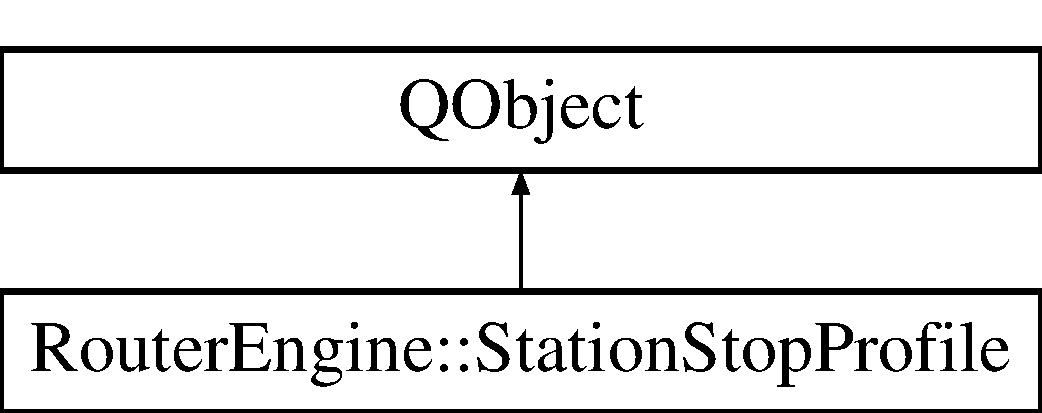
\includegraphics[height=2.000000cm]{classRouterEngine_1_1StationStopProfile}
\end{center}
\end{figure}
\subsection*{Signals}
\begin{DoxyCompactItemize}
\item 
\mbox{\Hypertarget{classRouterEngine_1_1StationStopProfile_ad33864259b9724e75d7f3187d233c5e5}\label{classRouterEngine_1_1StationStopProfile_ad33864259b9724e75d7f3187d233c5e5}} 
void {\bfseries departure\+Time\+Changed} ()
\item 
\mbox{\Hypertarget{classRouterEngine_1_1StationStopProfile_a9e7f64d4bd79947ee31a83152da41832}\label{classRouterEngine_1_1StationStopProfile_a9e7f64d4bd79947ee31a83152da41832}} 
void {\bfseries arrival\+Time\+Changed} ()
\item 
\mbox{\Hypertarget{classRouterEngine_1_1StationStopProfile_a84eeb659c20b5119c3020e8ed5d65b26}\label{classRouterEngine_1_1StationStopProfile_a84eeb659c20b5119c3020e8ed5d65b26}} 
void {\bfseries departure\+Connection\+Changed} ()
\item 
\mbox{\Hypertarget{classRouterEngine_1_1StationStopProfile_a6d5895b452b8af08cfa65633db189dd3}\label{classRouterEngine_1_1StationStopProfile_a6d5895b452b8af08cfa65633db189dd3}} 
void {\bfseries arrival\+Connection\+Changed} ()
\item 
\mbox{\Hypertarget{classRouterEngine_1_1StationStopProfile_ab102b2d4b7e4f8f9f987784006c6810c}\label{classRouterEngine_1_1StationStopProfile_ab102b2d4b7e4f8f9f987784006c6810c}} 
void {\bfseries transfers\+Changed} ()
\end{DoxyCompactItemize}
\subsection*{Public Member Functions}
\begin{DoxyCompactItemize}
\item 
\mbox{\Hypertarget{classRouterEngine_1_1StationStopProfile_a2a3218afe09a357c0d3285c8967d1869}\label{classRouterEngine_1_1StationStopProfile_a2a3218afe09a357c0d3285c8967d1869}} 
{\bfseries Station\+Stop\+Profile} (const Q\+Date\+Time \&departure\+Time, const Q\+Date\+Time \&arrival\+Time, \mbox{\hyperlink{classFragments_1_1Fragment}{Fragments\+::\+Fragment}} $\ast$departure\+Connection, \mbox{\hyperlink{classFragments_1_1Fragment}{Fragments\+::\+Fragment}} $\ast$arrival\+Connection, const qint16 transfers, Q\+Object $\ast$parent=nullptr)
\item 
\mbox{\Hypertarget{classRouterEngine_1_1StationStopProfile_a33812d3bad70605339ef02e9daf5420e}\label{classRouterEngine_1_1StationStopProfile_a33812d3bad70605339ef02e9daf5420e}} 
Q\+Date\+Time {\bfseries departure\+Time} () const
\item 
\mbox{\Hypertarget{classRouterEngine_1_1StationStopProfile_a9c734fbc59ba68448e725fd6c958f52e}\label{classRouterEngine_1_1StationStopProfile_a9c734fbc59ba68448e725fd6c958f52e}} 
void {\bfseries set\+Departure\+Time} (const Q\+Date\+Time \&departure\+Time)
\item 
\mbox{\Hypertarget{classRouterEngine_1_1StationStopProfile_ad578fd8f9e9d5040cd298050ea07400a}\label{classRouterEngine_1_1StationStopProfile_ad578fd8f9e9d5040cd298050ea07400a}} 
Q\+Date\+Time {\bfseries arrival\+Time} () const
\item 
\mbox{\Hypertarget{classRouterEngine_1_1StationStopProfile_a1e3def0943616522a1fdeeb17dba701a}\label{classRouterEngine_1_1StationStopProfile_a1e3def0943616522a1fdeeb17dba701a}} 
void {\bfseries set\+Arrival\+Time} (const Q\+Date\+Time \&arrival\+Time)
\item 
\mbox{\Hypertarget{classRouterEngine_1_1StationStopProfile_a78721007d3603be9e9ec705d5c41cd49}\label{classRouterEngine_1_1StationStopProfile_a78721007d3603be9e9ec705d5c41cd49}} 
\mbox{\hyperlink{classFragments_1_1Fragment}{Fragments\+::\+Fragment}} $\ast$ {\bfseries departure\+Connection} () const
\item 
\mbox{\Hypertarget{classRouterEngine_1_1StationStopProfile_acdd818e9cdc82cb6f54beab215de322e}\label{classRouterEngine_1_1StationStopProfile_acdd818e9cdc82cb6f54beab215de322e}} 
void {\bfseries set\+Departure\+Connection} (\mbox{\hyperlink{classFragments_1_1Fragment}{Fragments\+::\+Fragment}} $\ast$departure\+Connection)
\item 
\mbox{\Hypertarget{classRouterEngine_1_1StationStopProfile_a6ee8ca835f4e35c854f216feb04c18be}\label{classRouterEngine_1_1StationStopProfile_a6ee8ca835f4e35c854f216feb04c18be}} 
\mbox{\hyperlink{classFragments_1_1Fragment}{Fragments\+::\+Fragment}} $\ast$ {\bfseries arrival\+Connection} () const
\item 
\mbox{\Hypertarget{classRouterEngine_1_1StationStopProfile_acdd5cf23ce995fb0c00d511af94221be}\label{classRouterEngine_1_1StationStopProfile_acdd5cf23ce995fb0c00d511af94221be}} 
void {\bfseries set\+Arrival\+Connection} (\mbox{\hyperlink{classFragments_1_1Fragment}{Fragments\+::\+Fragment}} $\ast$arrival\+Connection)
\item 
\mbox{\Hypertarget{classRouterEngine_1_1StationStopProfile_a30cebe57a2d83b2bccc7096e718a20db}\label{classRouterEngine_1_1StationStopProfile_a30cebe57a2d83b2bccc7096e718a20db}} 
qint16 {\bfseries transfers} () const
\item 
\mbox{\Hypertarget{classRouterEngine_1_1StationStopProfile_a2ed64bade1f468a94185a14efd495e37}\label{classRouterEngine_1_1StationStopProfile_a2ed64bade1f468a94185a14efd495e37}} 
void {\bfseries set\+Transfers} (const qint16 \&transfers)
\end{DoxyCompactItemize}
\subsection*{Private Attributes}
\begin{DoxyCompactItemize}
\item 
\mbox{\Hypertarget{classRouterEngine_1_1StationStopProfile_a97eb98be57364fdd9e77e29de14579b5}\label{classRouterEngine_1_1StationStopProfile_a97eb98be57364fdd9e77e29de14579b5}} 
Q\+Date\+Time {\bfseries m\+\_\+departure\+Time}
\item 
\mbox{\Hypertarget{classRouterEngine_1_1StationStopProfile_a354f6857e93c542d6fbb08113d33e611}\label{classRouterEngine_1_1StationStopProfile_a354f6857e93c542d6fbb08113d33e611}} 
Q\+Date\+Time {\bfseries m\+\_\+arrival\+Time}
\item 
\mbox{\Hypertarget{classRouterEngine_1_1StationStopProfile_a99630a13e3e7fd440d28e61fa29ab56b}\label{classRouterEngine_1_1StationStopProfile_a99630a13e3e7fd440d28e61fa29ab56b}} 
\mbox{\hyperlink{classFragments_1_1Fragment}{Fragments\+::\+Fragment}} $\ast$ {\bfseries m\+\_\+departure\+Connection}
\item 
\mbox{\Hypertarget{classRouterEngine_1_1StationStopProfile_a7623369a846a96a0cf5fc3e9e23b8aaa}\label{classRouterEngine_1_1StationStopProfile_a7623369a846a96a0cf5fc3e9e23b8aaa}} 
\mbox{\hyperlink{classFragments_1_1Fragment}{Fragments\+::\+Fragment}} $\ast$ {\bfseries m\+\_\+arrival\+Connection}
\item 
\mbox{\Hypertarget{classRouterEngine_1_1StationStopProfile_adbafbfbe7205c1983575102a5eea0b53}\label{classRouterEngine_1_1StationStopProfile_adbafbfbe7205c1983575102a5eea0b53}} 
qint16 {\bfseries m\+\_\+transfers}
\end{DoxyCompactItemize}


The documentation for this class was generated from the following files\+:\begin{DoxyCompactItemize}
\item 
src/include/engines/router/routerstationstopprofile.\+h\item 
src/engines/router/\mbox{\hyperlink{routerstationstopprofile_8cpp}{routerstationstopprofile.\+cpp}}\end{DoxyCompactItemize}

\hypertarget{classVehicleEngine_1_1Stop}{}\section{Vehicle\+Engine\+:\+:Stop Class Reference}
\label{classVehicleEngine_1_1Stop}\index{Vehicle\+Engine\+::\+Stop@{Vehicle\+Engine\+::\+Stop}}
Inheritance diagram for Vehicle\+Engine\+:\+:Stop\+:\begin{figure}[H]
\begin{center}
\leavevmode
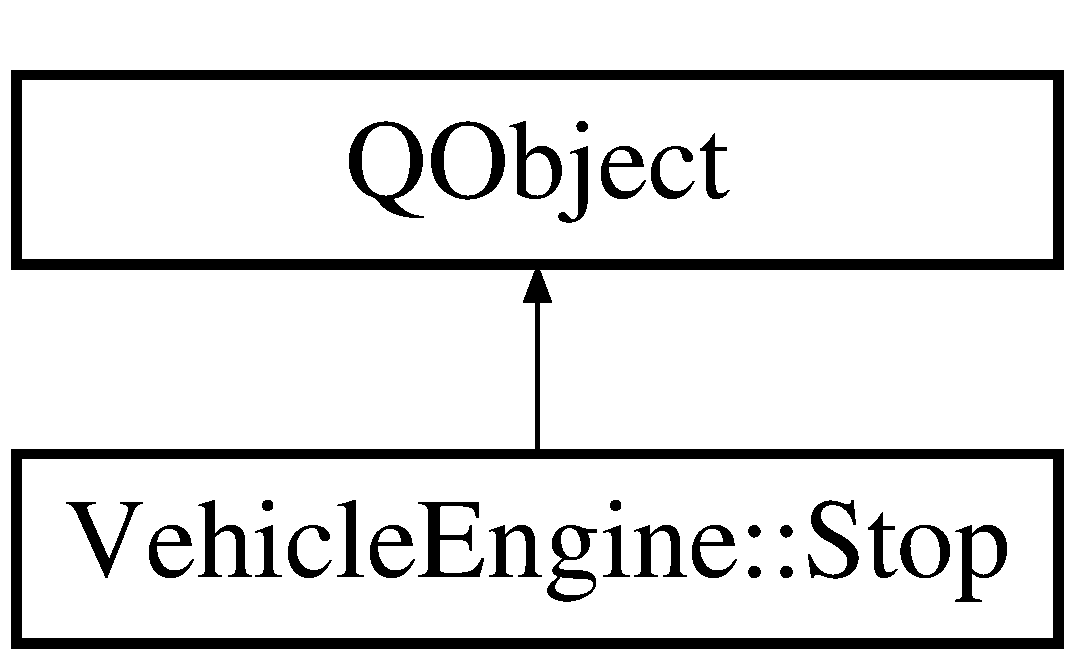
\includegraphics[height=2.000000cm]{classVehicleEngine_1_1Stop}
\end{center}
\end{figure}
\subsection*{Public Types}
\begin{DoxyCompactItemize}
\item 
\mbox{\Hypertarget{classVehicleEngine_1_1Stop_ae0c7ddc417639975e00b58181c3ee458}\label{classVehicleEngine_1_1Stop_ae0c7ddc417639975e00b58181c3ee458}} 
enum {\bfseries Type} \{ {\bfseries A\+R\+R\+I\+V\+AL}, 
{\bfseries D\+E\+P\+A\+R\+T\+U\+RE}, 
{\bfseries S\+T\+OP}, 
{\bfseries U\+N\+K\+N\+O\+WN}
 \}
\item 
\mbox{\Hypertarget{classVehicleEngine_1_1Stop_acdfae8b416558c41043261aaa02fdfe6}\label{classVehicleEngine_1_1Stop_acdfae8b416558c41043261aaa02fdfe6}} 
enum {\bfseries Occupancy\+Level} \{ \newline
{\bfseries U\+N\+S\+U\+P\+P\+O\+R\+T\+ED}, 
{\bfseries U\+N\+K\+N\+O\+WN}, 
{\bfseries L\+OW}, 
{\bfseries M\+E\+D\+I\+UM}, 
\newline
{\bfseries H\+I\+GH}
 \}
\end{DoxyCompactItemize}
\subsection*{Signals}
\begin{DoxyCompactItemize}
\item 
\mbox{\Hypertarget{classVehicleEngine_1_1Stop_a28011155a566266668c1fc939959d974}\label{classVehicleEngine_1_1Stop_a28011155a566266668c1fc939959d974}} 
void {\bfseries station\+Changed} ()
\item 
\mbox{\Hypertarget{classVehicleEngine_1_1Stop_ac090bda4b85a935d3f6ed4b1ad0c8ca7}\label{classVehicleEngine_1_1Stop_ac090bda4b85a935d3f6ed4b1ad0c8ca7}} 
void {\bfseries platform\+Changed} ()
\item 
\mbox{\Hypertarget{classVehicleEngine_1_1Stop_a60bf636375dabe9f7baa5d17d03af3ed}\label{classVehicleEngine_1_1Stop_a60bf636375dabe9f7baa5d17d03af3ed}} 
void {\bfseries is\+Platform\+Normal\+Changed} ()
\item 
\mbox{\Hypertarget{classVehicleEngine_1_1Stop_a17c68b7992490a38224e3a5d60fa1abc}\label{classVehicleEngine_1_1Stop_a17c68b7992490a38224e3a5d60fa1abc}} 
void {\bfseries has\+Left\+Changed} ()
\item 
\mbox{\Hypertarget{classVehicleEngine_1_1Stop_a580a8694f4fe7afab904fb57c7129039}\label{classVehicleEngine_1_1Stop_a580a8694f4fe7afab904fb57c7129039}} 
void {\bfseries departure\+Time\+Changed} ()
\item 
\mbox{\Hypertarget{classVehicleEngine_1_1Stop_a2fa5230630ea092be163683761584837}\label{classVehicleEngine_1_1Stop_a2fa5230630ea092be163683761584837}} 
void {\bfseries departure\+Delay\+Changed} ()
\item 
\mbox{\Hypertarget{classVehicleEngine_1_1Stop_a76c69b4d6ed8f200f0654ff51cf120f3}\label{classVehicleEngine_1_1Stop_a76c69b4d6ed8f200f0654ff51cf120f3}} 
void {\bfseries is\+Departure\+Canceled\+Changed} ()
\item 
\mbox{\Hypertarget{classVehicleEngine_1_1Stop_a96abb07fd64037cf2a797ae5a620b902}\label{classVehicleEngine_1_1Stop_a96abb07fd64037cf2a797ae5a620b902}} 
void {\bfseries arrival\+Time\+Changed} ()
\item 
\mbox{\Hypertarget{classVehicleEngine_1_1Stop_a2fa2b4c3d4f41e14d7e8c898fbae0ec4}\label{classVehicleEngine_1_1Stop_a2fa2b4c3d4f41e14d7e8c898fbae0ec4}} 
void {\bfseries arrival\+Delay\+Changed} ()
\item 
\mbox{\Hypertarget{classVehicleEngine_1_1Stop_accaa04f92666356ed48cfec72f341b1a}\label{classVehicleEngine_1_1Stop_accaa04f92666356ed48cfec72f341b1a}} 
void {\bfseries is\+Arrival\+Canceled\+Changed} ()
\item 
\mbox{\Hypertarget{classVehicleEngine_1_1Stop_a4c48ce2e195fd78cf0143eb39622633e}\label{classVehicleEngine_1_1Stop_a4c48ce2e195fd78cf0143eb39622633e}} 
void {\bfseries is\+Extra\+Stop\+Changed} ()
\item 
\mbox{\Hypertarget{classVehicleEngine_1_1Stop_a5cd6e6ecc6c6d88ead8e7a89afd9c684}\label{classVehicleEngine_1_1Stop_a5cd6e6ecc6c6d88ead8e7a89afd9c684}} 
void {\bfseries occupancy\+Level\+Changed} ()
\item 
\mbox{\Hypertarget{classVehicleEngine_1_1Stop_a0d6575b465d76e8bbabd125683111e1a}\label{classVehicleEngine_1_1Stop_a0d6575b465d76e8bbabd125683111e1a}} 
void {\bfseries type\+Changed} ()
\end{DoxyCompactItemize}
\subsection*{Public Member Functions}
\begin{DoxyCompactItemize}
\item 
\mbox{\Hypertarget{classVehicleEngine_1_1Stop_a0fc51aa36267d6fb067d8375d9c171b2}\label{classVehicleEngine_1_1Stop_a0fc51aa36267d6fb067d8375d9c171b2}} 
{\bfseries Stop} (Q\+Object $\ast$parent=nullptr)
\item 
\mbox{\Hypertarget{classVehicleEngine_1_1Stop_aeeccf29d98be9ccbe845a293738fa264}\label{classVehicleEngine_1_1Stop_aeeccf29d98be9ccbe845a293738fa264}} 
{\bfseries Stop} (\mbox{\hyperlink{classStationEngine_1_1Station}{Station\+Engine\+::\+Station}} $\ast$station, const Q\+String \&platform, const bool \&is\+Platform\+Normal, const bool \&has\+Left, const Q\+Date\+Time \&departure\+Time, const qint16 \&departure\+Delay, const bool \&is\+Departure\+Canceled, const Q\+Date\+Time \&arrival\+Time, const qint16 \&arrival\+Delay, const bool \&is\+Arrival\+Canceled, const bool \&is\+Extra\+Stop, const Vehicle\+Engine\+::\+Stop\+::\+Occupancy\+Level \&occupancy\+Level, const Vehicle\+Engine\+::\+Stop\+::\+Type \&type, Q\+Object $\ast$parent=nullptr)
\item 
\mbox{\Hypertarget{classVehicleEngine_1_1Stop_adadd380fc70cab6138d8804438f68dfa}\label{classVehicleEngine_1_1Stop_adadd380fc70cab6138d8804438f68dfa}} 
\mbox{\hyperlink{classStationEngine_1_1Station}{Station\+Engine\+::\+Station}} $\ast$ {\bfseries station} () const
\item 
\mbox{\Hypertarget{classVehicleEngine_1_1Stop_a3d9c4cdb63e71499efd6d7b7365c79db}\label{classVehicleEngine_1_1Stop_a3d9c4cdb63e71499efd6d7b7365c79db}} 
void {\bfseries set\+Station} (\mbox{\hyperlink{classStationEngine_1_1Station}{Station\+Engine\+::\+Station}} $\ast$station)
\item 
\mbox{\Hypertarget{classVehicleEngine_1_1Stop_a9e41b74478b3170c290821135350744c}\label{classVehicleEngine_1_1Stop_a9e41b74478b3170c290821135350744c}} 
Q\+String {\bfseries platform} () const
\item 
\mbox{\Hypertarget{classVehicleEngine_1_1Stop_a53858d3ec0183e9492b25427d4c694d0}\label{classVehicleEngine_1_1Stop_a53858d3ec0183e9492b25427d4c694d0}} 
void {\bfseries set\+Platform} (const Q\+String \&platform)
\item 
\mbox{\Hypertarget{classVehicleEngine_1_1Stop_a665852ce9a856667be28b3adc69f72c3}\label{classVehicleEngine_1_1Stop_a665852ce9a856667be28b3adc69f72c3}} 
bool {\bfseries is\+Platform\+Normal} () const
\item 
\mbox{\Hypertarget{classVehicleEngine_1_1Stop_ae87db218cc65ddff2768e8c7284a3b1e}\label{classVehicleEngine_1_1Stop_ae87db218cc65ddff2768e8c7284a3b1e}} 
void {\bfseries set\+Is\+Platform\+Normal} (const bool \&is\+Platform\+Normal)
\item 
\mbox{\Hypertarget{classVehicleEngine_1_1Stop_a5abdef3141a5ecae9f80bafcb2ef059a}\label{classVehicleEngine_1_1Stop_a5abdef3141a5ecae9f80bafcb2ef059a}} 
bool {\bfseries has\+Left} () const
\item 
\mbox{\Hypertarget{classVehicleEngine_1_1Stop_a2fb0dec57862278edcec9a0d5a299702}\label{classVehicleEngine_1_1Stop_a2fb0dec57862278edcec9a0d5a299702}} 
void {\bfseries set\+Has\+Left} (const bool \&has\+Left)
\item 
\mbox{\Hypertarget{classVehicleEngine_1_1Stop_a02e2288d7de6a29f1d1c0d0538da8af6}\label{classVehicleEngine_1_1Stop_a02e2288d7de6a29f1d1c0d0538da8af6}} 
Q\+Date\+Time {\bfseries departure\+Time} () const
\item 
\mbox{\Hypertarget{classVehicleEngine_1_1Stop_afd2e78ce7eaf448d5f62f98a037d42a4}\label{classVehicleEngine_1_1Stop_afd2e78ce7eaf448d5f62f98a037d42a4}} 
void {\bfseries set\+Departure\+Time} (const Q\+Date\+Time \&departure\+Time)
\item 
\mbox{\Hypertarget{classVehicleEngine_1_1Stop_a7b6c5d2802b9694dc3b01b5f6bf8f3dd}\label{classVehicleEngine_1_1Stop_a7b6c5d2802b9694dc3b01b5f6bf8f3dd}} 
qint16 {\bfseries departure\+Delay} () const
\item 
\mbox{\Hypertarget{classVehicleEngine_1_1Stop_a284ce9074018f03319855c12a1e831e9}\label{classVehicleEngine_1_1Stop_a284ce9074018f03319855c12a1e831e9}} 
void {\bfseries set\+Departure\+Delay} (const qint16 \&departure\+Delay)
\item 
\mbox{\Hypertarget{classVehicleEngine_1_1Stop_a59323c8dfb1c2715efeb00810ab99418}\label{classVehicleEngine_1_1Stop_a59323c8dfb1c2715efeb00810ab99418}} 
bool {\bfseries is\+Departure\+Canceled} () const
\item 
\mbox{\Hypertarget{classVehicleEngine_1_1Stop_aa609dc4b54e919f081da57754bbbf8d3}\label{classVehicleEngine_1_1Stop_aa609dc4b54e919f081da57754bbbf8d3}} 
void {\bfseries set\+Is\+Departure\+Canceled} (const bool \&is\+Departure\+Canceled)
\item 
\mbox{\Hypertarget{classVehicleEngine_1_1Stop_a473c5d32f259d7ec9096fd9b1938d915}\label{classVehicleEngine_1_1Stop_a473c5d32f259d7ec9096fd9b1938d915}} 
Q\+Date\+Time {\bfseries arrival\+Time} () const
\item 
\mbox{\Hypertarget{classVehicleEngine_1_1Stop_aba98fbc0338e7cb670c7b9448527f930}\label{classVehicleEngine_1_1Stop_aba98fbc0338e7cb670c7b9448527f930}} 
void {\bfseries set\+Arrival\+Time} (const Q\+Date\+Time \&arrival\+Time)
\item 
\mbox{\Hypertarget{classVehicleEngine_1_1Stop_a8e995e2fc7499d80173d4d1cd10d4dbb}\label{classVehicleEngine_1_1Stop_a8e995e2fc7499d80173d4d1cd10d4dbb}} 
qint16 {\bfseries arrival\+Delay} () const
\item 
\mbox{\Hypertarget{classVehicleEngine_1_1Stop_a20d19dc15cafbcbee2f1d785eded2ff9}\label{classVehicleEngine_1_1Stop_a20d19dc15cafbcbee2f1d785eded2ff9}} 
void {\bfseries set\+Arrival\+Delay} (const qint16 \&arrival\+Delay)
\item 
\mbox{\Hypertarget{classVehicleEngine_1_1Stop_a8972227e9ae5873a6654e02a32bd22b6}\label{classVehicleEngine_1_1Stop_a8972227e9ae5873a6654e02a32bd22b6}} 
bool {\bfseries is\+Arrival\+Canceled} () const
\item 
\mbox{\Hypertarget{classVehicleEngine_1_1Stop_a63f08dbf9b5414222d9c051aa92afe08}\label{classVehicleEngine_1_1Stop_a63f08dbf9b5414222d9c051aa92afe08}} 
void {\bfseries set\+Is\+Arrival\+Canceled} (const bool \&is\+Arrival\+Canceled)
\item 
\mbox{\Hypertarget{classVehicleEngine_1_1Stop_a5d9a2a26b199e711b3b98e384ed334ba}\label{classVehicleEngine_1_1Stop_a5d9a2a26b199e711b3b98e384ed334ba}} 
Vehicle\+Engine\+::\+Stop\+::\+Occupancy\+Level {\bfseries occupancy\+Level} () const
\item 
\mbox{\Hypertarget{classVehicleEngine_1_1Stop_a27bd665e9e64ecc2032e29d8ae037273}\label{classVehicleEngine_1_1Stop_a27bd665e9e64ecc2032e29d8ae037273}} 
void {\bfseries set\+Occupancy\+Level} (const Vehicle\+Engine\+::\+Stop\+::\+Occupancy\+Level \&occupancy\+Level)
\item 
\mbox{\Hypertarget{classVehicleEngine_1_1Stop_a25ba5081c1a2040c4394a6e2914c9069}\label{classVehicleEngine_1_1Stop_a25ba5081c1a2040c4394a6e2914c9069}} 
Vehicle\+Engine\+::\+Stop\+::\+Type {\bfseries type} () const
\item 
\mbox{\Hypertarget{classVehicleEngine_1_1Stop_a592019fa1501f1ac63f17b3d73841737}\label{classVehicleEngine_1_1Stop_a592019fa1501f1ac63f17b3d73841737}} 
void {\bfseries set\+Type} (const Vehicle\+Engine\+::\+Stop\+::\+Type \&type)
\item 
\mbox{\Hypertarget{classVehicleEngine_1_1Stop_a318dcdad4c17ea6598809691229e5070}\label{classVehicleEngine_1_1Stop_a318dcdad4c17ea6598809691229e5070}} 
bool {\bfseries is\+Extra\+Stop} () const
\item 
\mbox{\Hypertarget{classVehicleEngine_1_1Stop_afdcf6af7fe9638f8fb1caf1dd71df6a1}\label{classVehicleEngine_1_1Stop_afdcf6af7fe9638f8fb1caf1dd71df6a1}} 
void {\bfseries set\+Is\+Extra\+Stop} (const bool \&is\+Extra\+Stop)
\end{DoxyCompactItemize}
\subsection*{Private Attributes}
\begin{DoxyCompactItemize}
\item 
\mbox{\Hypertarget{classVehicleEngine_1_1Stop_a55b5bdb40835731950b91d55c64ff3fe}\label{classVehicleEngine_1_1Stop_a55b5bdb40835731950b91d55c64ff3fe}} 
\mbox{\hyperlink{classStationEngine_1_1Station}{Station\+Engine\+::\+Station}} $\ast$ {\bfseries m\+\_\+station}
\item 
\mbox{\Hypertarget{classVehicleEngine_1_1Stop_a0ec7b253aafb3b3ea9daf1bf99233f3e}\label{classVehicleEngine_1_1Stop_a0ec7b253aafb3b3ea9daf1bf99233f3e}} 
Q\+String {\bfseries m\+\_\+platform}
\item 
\mbox{\Hypertarget{classVehicleEngine_1_1Stop_abd6070c0ad5d83174803a626196e003e}\label{classVehicleEngine_1_1Stop_abd6070c0ad5d83174803a626196e003e}} 
bool {\bfseries m\+\_\+is\+Platform\+Normal}
\item 
\mbox{\Hypertarget{classVehicleEngine_1_1Stop_a5c3d5e134e85657263054be4d4445b6f}\label{classVehicleEngine_1_1Stop_a5c3d5e134e85657263054be4d4445b6f}} 
bool {\bfseries m\+\_\+has\+Left}
\item 
\mbox{\Hypertarget{classVehicleEngine_1_1Stop_a642eaa73dd202447df29bf15e74ecb27}\label{classVehicleEngine_1_1Stop_a642eaa73dd202447df29bf15e74ecb27}} 
Q\+Date\+Time {\bfseries m\+\_\+departure\+Time}
\item 
\mbox{\Hypertarget{classVehicleEngine_1_1Stop_ade5170166e85de34d929860e7ec8462b}\label{classVehicleEngine_1_1Stop_ade5170166e85de34d929860e7ec8462b}} 
qint16 {\bfseries m\+\_\+departure\+Delay}
\item 
\mbox{\Hypertarget{classVehicleEngine_1_1Stop_a3c86e5d98aaebc84f0c902de85eaebf1}\label{classVehicleEngine_1_1Stop_a3c86e5d98aaebc84f0c902de85eaebf1}} 
bool {\bfseries m\+\_\+is\+Departure\+Canceled}
\item 
\mbox{\Hypertarget{classVehicleEngine_1_1Stop_aaa18a1b4ea522d405440b372b40cf870}\label{classVehicleEngine_1_1Stop_aaa18a1b4ea522d405440b372b40cf870}} 
Q\+Date\+Time {\bfseries m\+\_\+arrival\+Time}
\item 
\mbox{\Hypertarget{classVehicleEngine_1_1Stop_a7b9ff6375e2f34aa24b552e1a8a30304}\label{classVehicleEngine_1_1Stop_a7b9ff6375e2f34aa24b552e1a8a30304}} 
qint16 {\bfseries m\+\_\+arrival\+Delay}
\item 
\mbox{\Hypertarget{classVehicleEngine_1_1Stop_ae80861122b29f10c983192d1f2443274}\label{classVehicleEngine_1_1Stop_ae80861122b29f10c983192d1f2443274}} 
bool {\bfseries m\+\_\+is\+Arrival\+Canceled}
\item 
\mbox{\Hypertarget{classVehicleEngine_1_1Stop_aba84b74fdf970bff43427887a7153d04}\label{classVehicleEngine_1_1Stop_aba84b74fdf970bff43427887a7153d04}} 
bool {\bfseries m\+\_\+is\+Extra\+Stop}
\item 
\mbox{\Hypertarget{classVehicleEngine_1_1Stop_a011edd566f330f6b7786a4839e2626c3}\label{classVehicleEngine_1_1Stop_a011edd566f330f6b7786a4839e2626c3}} 
Vehicle\+Engine\+::\+Stop\+::\+Occupancy\+Level {\bfseries m\+\_\+occupancy\+Level}
\item 
\mbox{\Hypertarget{classVehicleEngine_1_1Stop_ae65e93f8605a1a5b25383241da4749fe}\label{classVehicleEngine_1_1Stop_ae65e93f8605a1a5b25383241da4749fe}} 
Vehicle\+Engine\+::\+Stop\+::\+Type {\bfseries m\+\_\+type}
\end{DoxyCompactItemize}


The documentation for this class was generated from the following files\+:\begin{DoxyCompactItemize}
\item 
src/include/engines/vehicle/vehiclestop.\+h\item 
src/engines/vehicle/\mbox{\hyperlink{vehiclestop_8cpp}{vehiclestop.\+cpp}}\end{DoxyCompactItemize}

\hypertarget{classRouterEngine_1_1TrainProfile}{}\section{Router\+Engine\+:\+:Train\+Profile Class Reference}
\label{classRouterEngine_1_1TrainProfile}\index{Router\+Engine\+::\+Train\+Profile@{Router\+Engine\+::\+Train\+Profile}}
Inheritance diagram for Router\+Engine\+:\+:Train\+Profile\+:\begin{figure}[H]
\begin{center}
\leavevmode
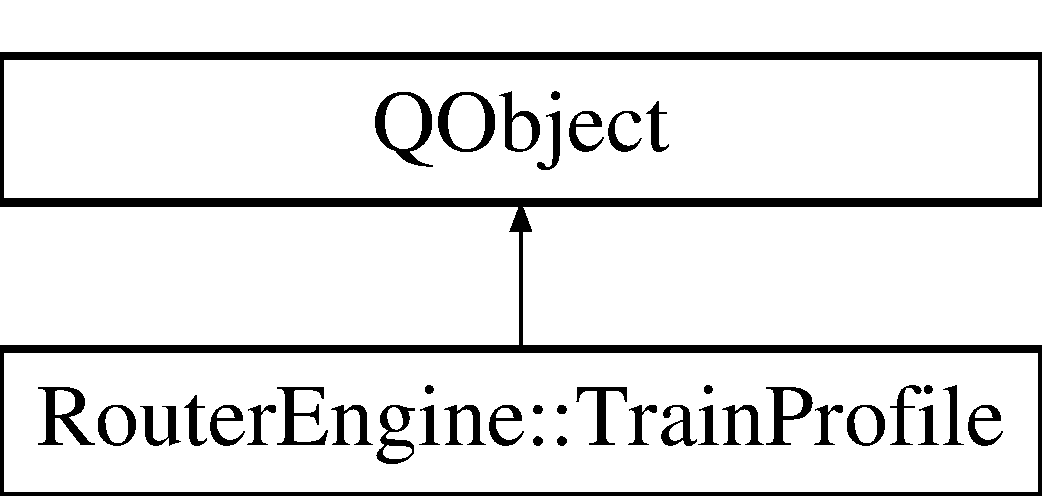
\includegraphics[height=2.000000cm]{classRouterEngine_1_1TrainProfile}
\end{center}
\end{figure}
\subsection*{Signals}
\begin{DoxyCompactItemize}
\item 
\mbox{\Hypertarget{classRouterEngine_1_1TrainProfile_afe0f0d59e98011a26d04182cc6c22f4b}\label{classRouterEngine_1_1TrainProfile_afe0f0d59e98011a26d04182cc6c22f4b}} 
void {\bfseries arrival\+Time\+Changed} ()
\item 
\mbox{\Hypertarget{classRouterEngine_1_1TrainProfile_ab15c6b13b788f6cceb3ec1ad6be6efc2}\label{classRouterEngine_1_1TrainProfile_ab15c6b13b788f6cceb3ec1ad6be6efc2}} 
void {\bfseries arrival\+Connection\+Changed} ()
\item 
\mbox{\Hypertarget{classRouterEngine_1_1TrainProfile_a8830ecbd04b1b6e9dae3123687faef87}\label{classRouterEngine_1_1TrainProfile_a8830ecbd04b1b6e9dae3123687faef87}} 
void {\bfseries transfers\+Changed} ()
\end{DoxyCompactItemize}
\subsection*{Public Member Functions}
\begin{DoxyCompactItemize}
\item 
\mbox{\Hypertarget{classRouterEngine_1_1TrainProfile_abe728c1cb1f8a8e280b6700beed6296c}\label{classRouterEngine_1_1TrainProfile_abe728c1cb1f8a8e280b6700beed6296c}} 
{\bfseries Train\+Profile} (const Q\+Date\+Time \&arrival\+Time, \mbox{\hyperlink{classFragments_1_1Fragment}{Fragments\+::\+Fragment}} $\ast$arrival\+Connection, const qint16 transfers, Q\+Object $\ast$parent=nullptr)
\item 
\mbox{\Hypertarget{classRouterEngine_1_1TrainProfile_a1b691f0fa3e969ecfd8693e0b1b5c6b7}\label{classRouterEngine_1_1TrainProfile_a1b691f0fa3e969ecfd8693e0b1b5c6b7}} 
Q\+Date\+Time {\bfseries arrival\+Time} () const
\item 
\mbox{\Hypertarget{classRouterEngine_1_1TrainProfile_a0fdb44416f8eb5298174516f33b8afaf}\label{classRouterEngine_1_1TrainProfile_a0fdb44416f8eb5298174516f33b8afaf}} 
void {\bfseries set\+Arrival\+Time} (const Q\+Date\+Time \&arrival\+Time)
\item 
\mbox{\Hypertarget{classRouterEngine_1_1TrainProfile_a58a6062ec5bac5ae68b4e7b3cc9536b3}\label{classRouterEngine_1_1TrainProfile_a58a6062ec5bac5ae68b4e7b3cc9536b3}} 
\mbox{\hyperlink{classFragments_1_1Fragment}{Fragments\+::\+Fragment}} $\ast$ {\bfseries arrival\+Connection} () const
\item 
\mbox{\Hypertarget{classRouterEngine_1_1TrainProfile_ad8087ee9128e34f41c28396036cb1999}\label{classRouterEngine_1_1TrainProfile_ad8087ee9128e34f41c28396036cb1999}} 
void {\bfseries set\+Arrival\+Connection} (\mbox{\hyperlink{classFragments_1_1Fragment}{Fragments\+::\+Fragment}} $\ast$arrival\+Connection)
\item 
\mbox{\Hypertarget{classRouterEngine_1_1TrainProfile_aa92906e1a0aed20b6e4d141bc3b4f418}\label{classRouterEngine_1_1TrainProfile_aa92906e1a0aed20b6e4d141bc3b4f418}} 
qint16 {\bfseries transfers} () const
\item 
\mbox{\Hypertarget{classRouterEngine_1_1TrainProfile_a4250ad7dd40ebaf9c37ba4c89824118b}\label{classRouterEngine_1_1TrainProfile_a4250ad7dd40ebaf9c37ba4c89824118b}} 
void {\bfseries set\+Transfers} (const qint16 \&transfers)
\end{DoxyCompactItemize}
\subsection*{Private Attributes}
\begin{DoxyCompactItemize}
\item 
\mbox{\Hypertarget{classRouterEngine_1_1TrainProfile_a5098409febd73d98a3d2093cbef8ca14}\label{classRouterEngine_1_1TrainProfile_a5098409febd73d98a3d2093cbef8ca14}} 
Q\+Date\+Time {\bfseries m\+\_\+arrival\+Time}
\item 
\mbox{\Hypertarget{classRouterEngine_1_1TrainProfile_a0e06b9aee6702dcdd4005ed46a3a342f}\label{classRouterEngine_1_1TrainProfile_a0e06b9aee6702dcdd4005ed46a3a342f}} 
\mbox{\hyperlink{classFragments_1_1Fragment}{Fragments\+::\+Fragment}} $\ast$ {\bfseries m\+\_\+arrival\+Connection}
\item 
\mbox{\Hypertarget{classRouterEngine_1_1TrainProfile_a59168106ca14045e79395be000c4012a}\label{classRouterEngine_1_1TrainProfile_a59168106ca14045e79395be000c4012a}} 
qint16 {\bfseries m\+\_\+transfers}
\end{DoxyCompactItemize}


The documentation for this class was generated from the following files\+:\begin{DoxyCompactItemize}
\item 
src/include/engines/router/routertrainprofile.\+h\item 
src/engines/router/\mbox{\hyperlink{routertrainprofile_8cpp}{routertrainprofile.\+cpp}}\end{DoxyCompactItemize}

\hypertarget{classRouterEngine_1_1Transfer}{}\section{Router\+Engine\+:\+:Transfer Class Reference}
\label{classRouterEngine_1_1Transfer}\index{Router\+Engine\+::\+Transfer@{Router\+Engine\+::\+Transfer}}
Inheritance diagram for Router\+Engine\+:\+:Transfer\+:\begin{figure}[H]
\begin{center}
\leavevmode
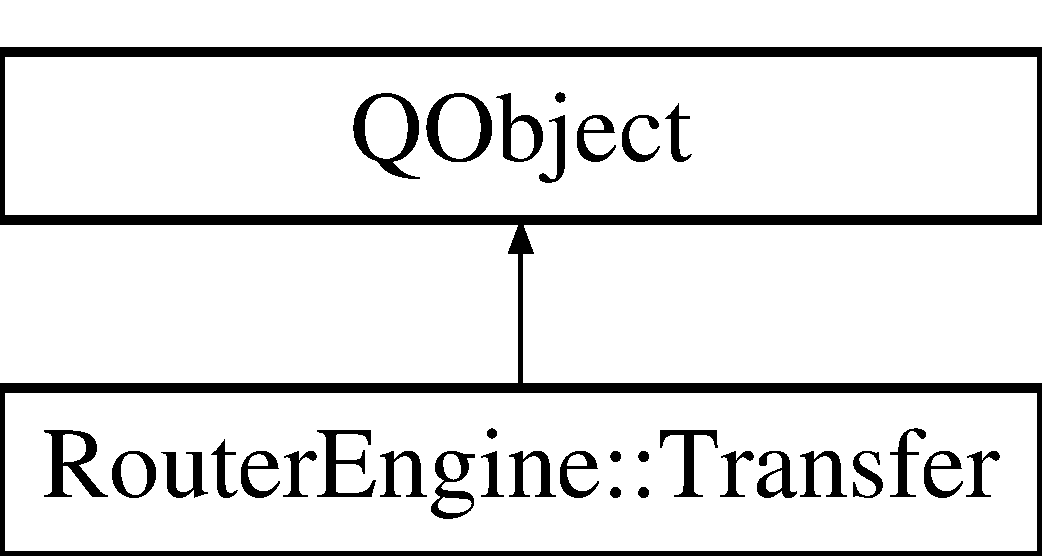
\includegraphics[height=2.000000cm]{classRouterEngine_1_1Transfer}
\end{center}
\end{figure}
\subsection*{Public Types}
\begin{DoxyCompactItemize}
\item 
\mbox{\Hypertarget{classRouterEngine_1_1Transfer_a2b79055b3dc55c7d9631a0d3e68155c5}\label{classRouterEngine_1_1Transfer_a2b79055b3dc55c7d9631a0d3e68155c5}} 
enum {\bfseries Type} \{ {\bfseries A\+R\+R\+I\+V\+AL}, 
{\bfseries D\+E\+P\+A\+R\+T\+U\+RE}, 
{\bfseries T\+R\+A\+N\+S\+F\+ER}, 
{\bfseries I\+N\+V\+A\+L\+ID}
 \}
\end{DoxyCompactItemize}
\subsection*{Signals}
\begin{DoxyCompactItemize}
\item 
\mbox{\Hypertarget{classRouterEngine_1_1Transfer_a727ff091ea2464cc1e6a5fa41dd38a9e}\label{classRouterEngine_1_1Transfer_a727ff091ea2464cc1e6a5fa41dd38a9e}} 
void {\bfseries departure\+Leg\+Changed} ()
\item 
\mbox{\Hypertarget{classRouterEngine_1_1Transfer_a40b2a38cb0fcc48cc867409139242655}\label{classRouterEngine_1_1Transfer_a40b2a38cb0fcc48cc867409139242655}} 
void {\bfseries arrival\+Leg\+Changed} ()
\item 
\mbox{\Hypertarget{classRouterEngine_1_1Transfer_ad82484af56ccf65ef26862da23f96e78}\label{classRouterEngine_1_1Transfer_ad82484af56ccf65ef26862da23f96e78}} 
void {\bfseries departure\+Changed} ()
\item 
\mbox{\Hypertarget{classRouterEngine_1_1Transfer_a7832205361f2f6273d2de37a33f8e5ac}\label{classRouterEngine_1_1Transfer_a7832205361f2f6273d2de37a33f8e5ac}} 
void {\bfseries arrival\+Changed} ()
\item 
\mbox{\Hypertarget{classRouterEngine_1_1Transfer_a366c6e5188577967c89d4c52898cc652}\label{classRouterEngine_1_1Transfer_a366c6e5188577967c89d4c52898cc652}} 
void {\bfseries type\+Changed} ()
\end{DoxyCompactItemize}
\subsection*{Public Member Functions}
\begin{DoxyCompactItemize}
\item 
\mbox{\Hypertarget{classRouterEngine_1_1Transfer_a4dfa4a9e6d843c7a2a050e0767560917}\label{classRouterEngine_1_1Transfer_a4dfa4a9e6d843c7a2a050e0767560917}} 
{\bfseries Transfer} (\mbox{\hyperlink{classRouterEngine_1_1RouteLeg}{Router\+Engine\+::\+Route\+Leg}} $\ast$departure\+Leg=nullptr, \mbox{\hyperlink{classRouterEngine_1_1RouteLeg}{Router\+Engine\+::\+Route\+Leg}} $\ast$arrival\+Leg=nullptr, Q\+Object $\ast$parent=nullptr)
\item 
\mbox{\Hypertarget{classRouterEngine_1_1Transfer_ab4ba2b3ce728923052331bf326fe5ee4}\label{classRouterEngine_1_1Transfer_ab4ba2b3ce728923052331bf326fe5ee4}} 
\mbox{\hyperlink{classRouterEngine_1_1RouteLeg}{Router\+Engine\+::\+Route\+Leg}} $\ast$ {\bfseries departure\+Leg} () const
\item 
\mbox{\Hypertarget{classRouterEngine_1_1Transfer_a0a21c2e3ea7d76323445a942820a36cc}\label{classRouterEngine_1_1Transfer_a0a21c2e3ea7d76323445a942820a36cc}} 
void {\bfseries set\+Departure\+Leg} (\mbox{\hyperlink{classRouterEngine_1_1RouteLeg}{Router\+Engine\+::\+Route\+Leg}} $\ast$departure\+Leg)
\item 
\mbox{\Hypertarget{classRouterEngine_1_1Transfer_a1eb0676f65b56cb2669c5273524ee87d}\label{classRouterEngine_1_1Transfer_a1eb0676f65b56cb2669c5273524ee87d}} 
\mbox{\hyperlink{classRouterEngine_1_1RouteLeg}{Router\+Engine\+::\+Route\+Leg}} $\ast$ {\bfseries arrival\+Leg} () const
\item 
\mbox{\Hypertarget{classRouterEngine_1_1Transfer_aaf6ae64e23f5b6a21b445c16810bdbd0}\label{classRouterEngine_1_1Transfer_aaf6ae64e23f5b6a21b445c16810bdbd0}} 
void {\bfseries set\+Arrival\+Leg} (\mbox{\hyperlink{classRouterEngine_1_1RouteLeg}{Router\+Engine\+::\+Route\+Leg}} $\ast$arrival\+Leg)
\item 
\mbox{\Hypertarget{classRouterEngine_1_1Transfer_a9de49b6229b08774c59a35e069241382}\label{classRouterEngine_1_1Transfer_a9de49b6229b08774c59a35e069241382}} 
\mbox{\hyperlink{classRouterEngine_1_1RouteLegEnd}{Router\+Engine\+::\+Route\+Leg\+End}} $\ast$ {\bfseries departure} () const
\item 
\mbox{\Hypertarget{classRouterEngine_1_1Transfer_a07c651c052bcc4d12adf1d8fe8558473}\label{classRouterEngine_1_1Transfer_a07c651c052bcc4d12adf1d8fe8558473}} 
void {\bfseries set\+Departure} (\mbox{\hyperlink{classRouterEngine_1_1RouteLegEnd}{Router\+Engine\+::\+Route\+Leg\+End}} $\ast$departure)
\item 
\mbox{\Hypertarget{classRouterEngine_1_1Transfer_add9dd9f32aeb0a03643b4b3c7f9af752}\label{classRouterEngine_1_1Transfer_add9dd9f32aeb0a03643b4b3c7f9af752}} 
\mbox{\hyperlink{classRouterEngine_1_1RouteLegEnd}{Router\+Engine\+::\+Route\+Leg\+End}} $\ast$ {\bfseries arrival} () const
\item 
\mbox{\Hypertarget{classRouterEngine_1_1Transfer_acbb38fde6669e70006edd8cfadda4aa9}\label{classRouterEngine_1_1Transfer_acbb38fde6669e70006edd8cfadda4aa9}} 
void {\bfseries set\+Arrival} (\mbox{\hyperlink{classRouterEngine_1_1RouteLegEnd}{Router\+Engine\+::\+Route\+Leg\+End}} $\ast$arrival)
\item 
\mbox{\Hypertarget{classRouterEngine_1_1Transfer_aa68b42bfaacfe79b9d085c6a94aae2f8}\label{classRouterEngine_1_1Transfer_aa68b42bfaacfe79b9d085c6a94aae2f8}} 
Router\+Engine\+::\+Transfer\+::\+Type {\bfseries type} () const
\item 
\mbox{\Hypertarget{classRouterEngine_1_1Transfer_a2fd8d8f407490ad51b4604b3b379230e}\label{classRouterEngine_1_1Transfer_a2fd8d8f407490ad51b4604b3b379230e}} 
void {\bfseries set\+Type} (const Router\+Engine\+::\+Transfer\+::\+Type \&type)
\item 
\mbox{\Hypertarget{classRouterEngine_1_1Transfer_a9951403dc91e9e9be8a11cef284f7df8}\label{classRouterEngine_1_1Transfer_a9951403dc91e9e9be8a11cef284f7df8}} 
Q\+Url {\bfseries uri} () const
\item 
\mbox{\Hypertarget{classRouterEngine_1_1Transfer_a25dc4c790111fea727fdfe37413d0600}\label{classRouterEngine_1_1Transfer_a25dc4c790111fea727fdfe37413d0600}} 
\mbox{\hyperlink{classStationEngine_1_1Station}{Station\+Engine\+::\+Station}} $\ast$ {\bfseries station} () const
\item 
\mbox{\Hypertarget{classRouterEngine_1_1Transfer_ae3a407001d9a4f1324dc4421d5d41bfb}\label{classRouterEngine_1_1Transfer_ae3a407001d9a4f1324dc4421d5d41bfb}} 
Q\+Date\+Time {\bfseries time} () const
\item 
\mbox{\Hypertarget{classRouterEngine_1_1Transfer_a0453774c1c6b2ba31cb2aafdaa60487d}\label{classRouterEngine_1_1Transfer_a0453774c1c6b2ba31cb2aafdaa60487d}} 
qint16 {\bfseries delay} () const
\item 
\mbox{\Hypertarget{classRouterEngine_1_1Transfer_a20b15b42fe19d1cf2d139b33242c7d02}\label{classRouterEngine_1_1Transfer_a20b15b42fe19d1cf2d139b33242c7d02}} 
Q\+Date\+Time {\bfseries delayed\+Time} () const
\item 
\mbox{\Hypertarget{classRouterEngine_1_1Transfer_a74ddb24be5e96f945a7ac946b1201e9e}\label{classRouterEngine_1_1Transfer_a74ddb24be5e96f945a7ac946b1201e9e}} 
Q\+String {\bfseries platform} () const
\item 
\mbox{\Hypertarget{classRouterEngine_1_1Transfer_aff9e03cce26d0bee9e8871b796f5b0f3}\label{classRouterEngine_1_1Transfer_aff9e03cce26d0bee9e8871b796f5b0f3}} 
bool {\bfseries is\+Canceled} () const
\item 
\mbox{\Hypertarget{classRouterEngine_1_1Transfer_aafcb639e843877555b6181ce8fe05e3c}\label{classRouterEngine_1_1Transfer_aafcb639e843877555b6181ce8fe05e3c}} 
bool {\bfseries is\+Normal\+Platform} () const
\item 
\mbox{\Hypertarget{classRouterEngine_1_1Transfer_adb3a0639e91faff1efed72fd37732f47}\label{classRouterEngine_1_1Transfer_adb3a0639e91faff1efed72fd37732f47}} 
bool {\bfseries is\+Passed} () const
\item 
\mbox{\Hypertarget{classRouterEngine_1_1Transfer_ac5a0ffecfe78455585ff85c221e3441c}\label{classRouterEngine_1_1Transfer_ac5a0ffecfe78455585ff85c221e3441c}} 
Vehicle\+Engine\+::\+Stop\+::\+Occupancy\+Level {\bfseries occupancy\+Level} () const
\end{DoxyCompactItemize}
\subsection*{Private Attributes}
\begin{DoxyCompactItemize}
\item 
\mbox{\Hypertarget{classRouterEngine_1_1Transfer_a40772fc03d985aa0f8820c9ad414e50a}\label{classRouterEngine_1_1Transfer_a40772fc03d985aa0f8820c9ad414e50a}} 
\mbox{\hyperlink{classRouterEngine_1_1RouteLeg}{Router\+Engine\+::\+Route\+Leg}} $\ast$ {\bfseries m\+\_\+departure\+Leg}
\item 
\mbox{\Hypertarget{classRouterEngine_1_1Transfer_a3104b73a0130558587111a7ec4a6cfff}\label{classRouterEngine_1_1Transfer_a3104b73a0130558587111a7ec4a6cfff}} 
\mbox{\hyperlink{classRouterEngine_1_1RouteLeg}{Router\+Engine\+::\+Route\+Leg}} $\ast$ {\bfseries m\+\_\+arrival\+Leg}
\item 
\mbox{\Hypertarget{classRouterEngine_1_1Transfer_ac33555843efa0815443c47324c55480c}\label{classRouterEngine_1_1Transfer_ac33555843efa0815443c47324c55480c}} 
\mbox{\hyperlink{classRouterEngine_1_1RouteLegEnd}{Router\+Engine\+::\+Route\+Leg\+End}} $\ast$ {\bfseries m\+\_\+departure}
\item 
\mbox{\Hypertarget{classRouterEngine_1_1Transfer_a28ddd26907a602c03614ff89c78667ef}\label{classRouterEngine_1_1Transfer_a28ddd26907a602c03614ff89c78667ef}} 
\mbox{\hyperlink{classRouterEngine_1_1RouteLegEnd}{Router\+Engine\+::\+Route\+Leg\+End}} $\ast$ {\bfseries m\+\_\+arrival}
\item 
\mbox{\Hypertarget{classRouterEngine_1_1Transfer_a029f1581f2c05784924898946fff9dc3}\label{classRouterEngine_1_1Transfer_a029f1581f2c05784924898946fff9dc3}} 
Router\+Engine\+::\+Transfer\+::\+Type {\bfseries m\+\_\+type}
\end{DoxyCompactItemize}


The documentation for this class was generated from the following files\+:\begin{DoxyCompactItemize}
\item 
src/include/engines/router/routertransfer.\+h\item 
src/engines/router/\mbox{\hyperlink{routertransfer_8cpp}{routertransfer.\+cpp}}\end{DoxyCompactItemize}

\hypertarget{classVehicleEngine_1_1Vehicle}{}\section{Vehicle\+Engine\+:\+:Vehicle Class Reference}
\label{classVehicleEngine_1_1Vehicle}\index{Vehicle\+Engine\+::\+Vehicle@{Vehicle\+Engine\+::\+Vehicle}}
Inheritance diagram for Vehicle\+Engine\+:\+:Vehicle\+:\begin{figure}[H]
\begin{center}
\leavevmode
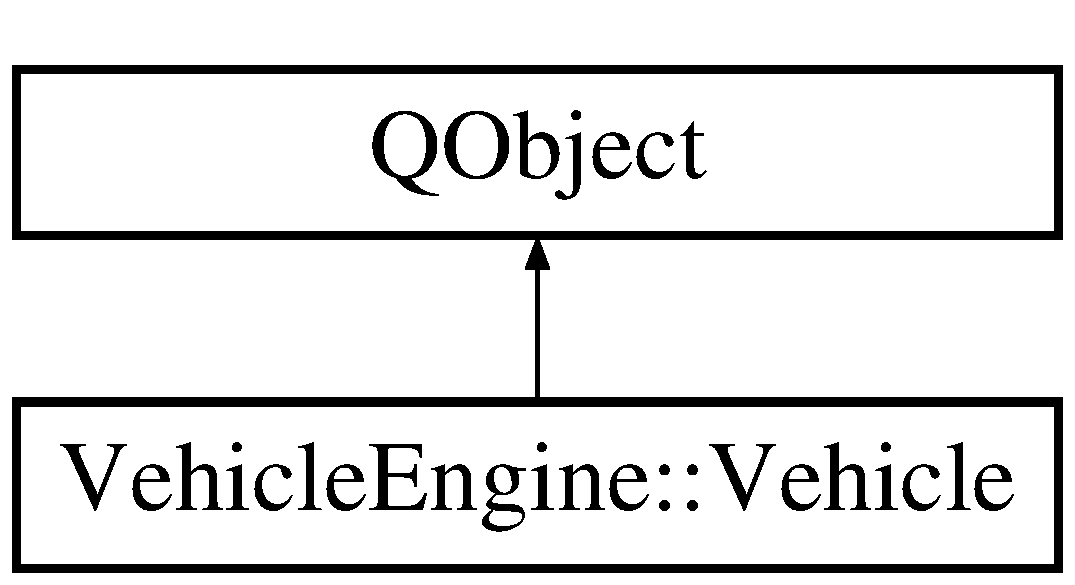
\includegraphics[height=2.000000cm]{classVehicleEngine_1_1Vehicle}
\end{center}
\end{figure}
\subsection*{Signals}
\begin{DoxyCompactItemize}
\item 
\mbox{\Hypertarget{classVehicleEngine_1_1Vehicle_a424944591db3168c779f29e7a57f53d3}\label{classVehicleEngine_1_1Vehicle_a424944591db3168c779f29e7a57f53d3}} 
void {\bfseries uri\+Changed} ()
\item 
\mbox{\Hypertarget{classVehicleEngine_1_1Vehicle_a6326f1db5b6232dab0102aa5023a4c4c}\label{classVehicleEngine_1_1Vehicle_a6326f1db5b6232dab0102aa5023a4c4c}} 
void {\bfseries trip\+U\+R\+I\+Changed} ()
\item 
\mbox{\Hypertarget{classVehicleEngine_1_1Vehicle_af99cdf961767ec0c230936ed062017de}\label{classVehicleEngine_1_1Vehicle_af99cdf961767ec0c230936ed062017de}} 
void {\bfseries headsign\+Changed} ()
\item 
\mbox{\Hypertarget{classVehicleEngine_1_1Vehicle_a7e493b3cb817e60368bff73d6e09b4c9}\label{classVehicleEngine_1_1Vehicle_a7e493b3cb817e60368bff73d6e09b4c9}} 
void {\bfseries intermediary\+Stops\+Changed} ()
\end{DoxyCompactItemize}
\subsection*{Public Member Functions}
\begin{DoxyCompactItemize}
\item 
\mbox{\Hypertarget{classVehicleEngine_1_1Vehicle_a208c46e84099d0f24ebcf699aedf9ca2}\label{classVehicleEngine_1_1Vehicle_a208c46e84099d0f24ebcf699aedf9ca2}} 
{\bfseries Vehicle} (Q\+Object $\ast$parent=nullptr)
\item 
\mbox{\Hypertarget{classVehicleEngine_1_1Vehicle_a637a49b74131270fdf0d73a6268e2716}\label{classVehicleEngine_1_1Vehicle_a637a49b74131270fdf0d73a6268e2716}} 
{\bfseries Vehicle} (const Q\+Url \&uri, const Q\+Url \&trip\+U\+RI, const Q\+String \&headsign, Q\+Object $\ast$parent=nullptr)
\item 
\mbox{\Hypertarget{classVehicleEngine_1_1Vehicle_ac3b5f107da52e20512f9fca88a9ef3b3}\label{classVehicleEngine_1_1Vehicle_ac3b5f107da52e20512f9fca88a9ef3b3}} 
{\bfseries Vehicle} (const Q\+Url \&uri, const Q\+Url \&trip\+U\+RI, const Q\+String \&headsign, const Q\+List$<$ \mbox{\hyperlink{classVehicleEngine_1_1Stop}{Vehicle\+Engine\+::\+Stop}} $\ast$$>$ \&intermediary\+Stops, Q\+Object $\ast$parent=nullptr)
\item 
\mbox{\Hypertarget{classVehicleEngine_1_1Vehicle_aa28bd729ce87ee0640c774f84a1ff93c}\label{classVehicleEngine_1_1Vehicle_aa28bd729ce87ee0640c774f84a1ff93c}} 
Q\+Url {\bfseries uri} () const
\item 
\mbox{\Hypertarget{classVehicleEngine_1_1Vehicle_a8196649a042f595230bb09b345d2ef18}\label{classVehicleEngine_1_1Vehicle_a8196649a042f595230bb09b345d2ef18}} 
void {\bfseries set\+Uri} (const Q\+Url \&uri)
\item 
\mbox{\Hypertarget{classVehicleEngine_1_1Vehicle_a4c9503af7c7b35d2d5cfbc20f8601209}\label{classVehicleEngine_1_1Vehicle_a4c9503af7c7b35d2d5cfbc20f8601209}} 
Q\+String {\bfseries headsign} () const
\item 
\mbox{\Hypertarget{classVehicleEngine_1_1Vehicle_abaeb138ff93f006df951c6f2ca7e352a}\label{classVehicleEngine_1_1Vehicle_abaeb138ff93f006df951c6f2ca7e352a}} 
void {\bfseries set\+Headsign} (const Q\+String \&headsign)
\item 
\mbox{\Hypertarget{classVehicleEngine_1_1Vehicle_a205ffe1cda249e0c888c9f925c6b7e9b}\label{classVehicleEngine_1_1Vehicle_a205ffe1cda249e0c888c9f925c6b7e9b}} 
Q\+List$<$ \mbox{\hyperlink{classVehicleEngine_1_1Stop}{Vehicle\+Engine\+::\+Stop}} $\ast$ $>$ {\bfseries intermediary\+Stops} () const
\item 
\mbox{\Hypertarget{classVehicleEngine_1_1Vehicle_ad2c644c2414a66b3a222620fcbf536ff}\label{classVehicleEngine_1_1Vehicle_ad2c644c2414a66b3a222620fcbf536ff}} 
void {\bfseries set\+Intermediary\+Stops} (const Q\+List$<$ \mbox{\hyperlink{classVehicleEngine_1_1Stop}{Vehicle\+Engine\+::\+Stop}} $\ast$$>$ \&intermediary\+Stops)
\item 
\mbox{\Hypertarget{classVehicleEngine_1_1Vehicle_ab5b7daeb46c8f0b1c080fc4141e2018b}\label{classVehicleEngine_1_1Vehicle_ab5b7daeb46c8f0b1c080fc4141e2018b}} 
Q\+Url {\bfseries trip\+U\+RI} () const
\item 
\mbox{\Hypertarget{classVehicleEngine_1_1Vehicle_a6d1d511465c92754999b20adba56ec61}\label{classVehicleEngine_1_1Vehicle_a6d1d511465c92754999b20adba56ec61}} 
void {\bfseries set\+Trip\+U\+RI} (const Q\+Url \&trip\+U\+RI)
\end{DoxyCompactItemize}
\subsection*{Private Attributes}
\begin{DoxyCompactItemize}
\item 
\mbox{\Hypertarget{classVehicleEngine_1_1Vehicle_a6edf7c8ad9c1e2d613f4815d4075141a}\label{classVehicleEngine_1_1Vehicle_a6edf7c8ad9c1e2d613f4815d4075141a}} 
Q\+Url {\bfseries m\+\_\+uri}
\item 
\mbox{\Hypertarget{classVehicleEngine_1_1Vehicle_a85bbbb01dc06798d44f0af97eb438b66}\label{classVehicleEngine_1_1Vehicle_a85bbbb01dc06798d44f0af97eb438b66}} 
Q\+Url {\bfseries m\+\_\+trip\+U\+RI}
\item 
\mbox{\Hypertarget{classVehicleEngine_1_1Vehicle_a7267b7a62e44238959665efaee646f92}\label{classVehicleEngine_1_1Vehicle_a7267b7a62e44238959665efaee646f92}} 
Q\+String {\bfseries m\+\_\+headsign}
\item 
\mbox{\Hypertarget{classVehicleEngine_1_1Vehicle_ab287cb6c07de0f514d3076cac6f7eb5b}\label{classVehicleEngine_1_1Vehicle_ab287cb6c07de0f514d3076cac6f7eb5b}} 
Q\+List$<$ \mbox{\hyperlink{classVehicleEngine_1_1Stop}{Vehicle\+Engine\+::\+Stop}} $\ast$ $>$ {\bfseries m\+\_\+intermediary\+Stops}
\end{DoxyCompactItemize}


The documentation for this class was generated from the following files\+:\begin{DoxyCompactItemize}
\item 
src/include/engines/vehicle/vehiclevehicle.\+h\item 
src/engines/vehicle/\mbox{\hyperlink{vehiclevehicle_8cpp}{vehiclevehicle.\+cpp}}\end{DoxyCompactItemize}

\chapter{File Documentation}
\hypertarget{databasemanager_8cpp}{}\section{src/database/databasemanager.cpp File Reference}
\label{databasemanager_8cpp}\index{src/database/databasemanager.\+cpp@{src/database/databasemanager.\+cpp}}


Manager facade constructor.  


{\ttfamily \#include \char`\"{}database/databasemanager.\+h\char`\"{}}\newline
\subsection*{Namespaces}
\begin{DoxyCompactItemize}
\item 
 \mbox{\hyperlink{namespaceDatabase}{Database}}
\end{DoxyCompactItemize}


\subsection{Detailed Description}
Manager facade constructor. 

Gets the current Q\+Sql\+Database database.

Sets the Q\+Sql\+Database database.

Ends the transaction.

Starts the transaction.

Executes a given Q\+Sql\+Query asynchronous.

Executes a given Q\+Sql\+Query.

Gets a \mbox{\hyperlink{classDatabase_1_1Manager}{Database\+::\+Manager}} instance.

\begin{DoxyAuthor}{Author}
Dylan Van Assche 
\end{DoxyAuthor}
\begin{DoxyDate}{Date}
20 Jul 2018 
\end{DoxyDate}

\begin{DoxyParams}{Parameters}
{\em Q\+Object} & $\ast$parent \\
\hline
{\em Q\+String} & path\\
\hline
\end{DoxyParams}
\begin{DoxyAuthor}{Author}
Dylan Van Assche 
\end{DoxyAuthor}
\begin{DoxyDate}{Date}
21 Jul 2018 
\end{DoxyDate}
\begin{DoxyReturn}{Returns}
\mbox{\hyperlink{classDatabase_1_1Manager}{Database\+::\+Manager}} $\ast$manager
\end{DoxyReturn}
\begin{DoxyAuthor}{Author}
Dylan Van Assche 
\end{DoxyAuthor}
\begin{DoxyDate}{Date}
20 Jul 2018 
\end{DoxyDate}

\begin{DoxyParams}{Parameters}
{\em Q\+Sql\+Query} & query \\
\hline
\end{DoxyParams}
\begin{DoxyReturn}{Returns}
bool success
\end{DoxyReturn}
\begin{DoxyAuthor}{Author}
Dylan Van Assche 
\end{DoxyAuthor}
\begin{DoxyDate}{Date}
13 Aug 2018 
\end{DoxyDate}

\begin{DoxyParams}{Parameters}
{\em Q\+Sql\+Query} & query \\
\hline
\end{DoxyParams}
\begin{DoxyReturn}{Returns}
bool success
\end{DoxyReturn}
\begin{DoxyAuthor}{Author}
Dylan Van Assche 
\end{DoxyAuthor}
\begin{DoxyDate}{Date}
9 Aug 2018 
\end{DoxyDate}
\begin{DoxyReturn}{Returns}
bool success
\end{DoxyReturn}
\begin{DoxyAuthor}{Author}
Dylan Van Assche 
\end{DoxyAuthor}
\begin{DoxyDate}{Date}
20 Jul 2018 
\end{DoxyDate}

\begin{DoxyParams}{Parameters}
{\em const} & Q\+Sql\+Database \&database\\
\hline
\end{DoxyParams}
\begin{DoxyAuthor}{Author}
Dylan Van Assche 
\end{DoxyAuthor}
\begin{DoxyDate}{Date}
20 Jul 2018 
\end{DoxyDate}
\begin{DoxyReturn}{Returns}
Q\+Sql\+Database database 
\end{DoxyReturn}

\hypertarget{alertsmessage_8cpp}{}\section{src/engines/alerts/alertsmessage.cpp File Reference}
\label{alertsmessage_8cpp}\index{src/engines/alerts/alertsmessage.cpp@{src/engines/alerts/alertsmessage.cpp}}


Sets the description.  


{\ttfamily \#include \char`\"{}engines/alerts/alertsmessage.\+h\char`\"{}}\newline
\subsection*{Namespaces}
\begin{DoxyCompactItemize}
\item 
 \mbox{\hyperlink{namespaceAlertsEngine}{Alerts\+Engine}}
\begin{DoxyCompactList}\small\item\em Sets the description of the message to the given Q\+String \&description. \end{DoxyCompactList}\end{DoxyCompactItemize}


\subsection{Detailed Description}
Sets the description. 

Sets the link.

Gets the link.

Sets the lead.

Gets the lead.

\begin{DoxyAuthor}{Author}
Dylan Van Assche 
\end{DoxyAuthor}
\begin{DoxyDate}{Date}
09 Aug 2018 
\end{DoxyDate}

\begin{DoxyParams}{Parameters}
{\em const} & Q\+String \&description\\
\hline
\end{DoxyParams}
\begin{DoxyAuthor}{Author}
Dylan Van Assche 
\end{DoxyAuthor}
\begin{DoxyDate}{Date}
09 Aug 2018 
\end{DoxyDate}
\begin{DoxyReturn}{Returns}
const Q\+String lead
\end{DoxyReturn}
\begin{DoxyAuthor}{Author}
Dylan Van Assche 
\end{DoxyAuthor}
\begin{DoxyDate}{Date}
09 Aug 2018 
\end{DoxyDate}

\begin{DoxyParams}{Parameters}
{\em const} & Q\+String \&lead\\
\hline
\end{DoxyParams}
\begin{DoxyAuthor}{Author}
Dylan Van Assche 
\end{DoxyAuthor}
\begin{DoxyDate}{Date}
09 Aug 2018 
\end{DoxyDate}
\begin{DoxyReturn}{Returns}
const Q\+Url link
\end{DoxyReturn}
\begin{DoxyAuthor}{Author}
Dylan Van Assche 
\end{DoxyAuthor}
\begin{DoxyDate}{Date}
09 Aug 2018 
\end{DoxyDate}

\begin{DoxyParams}{Parameters}
{\em const} & Q\+Url \&link \\
\hline
\end{DoxyParams}

\hypertarget{liveboardboard_8cpp}{}\section{src/engines/liveboard/liveboardboard.cpp File Reference}
\label{liveboardboard_8cpp}\index{src/engines/liveboard/liveboardboard.cpp@{src/engines/liveboard/liveboardboard.cpp}}


Gets the until time.  


{\ttfamily \#include \char`\"{}engines/liveboard/liveboardboard.\+h\char`\"{}}\newline
\subsection*{Namespaces}
\begin{DoxyCompactItemize}
\item 
 \mbox{\hyperlink{namespaceLiveboard}{Liveboard}}
\begin{DoxyCompactList}\small\item\em Gets the until time and returns it. \end{DoxyCompactList}\end{DoxyCompactItemize}


\subsection{Detailed Description}
Gets the until time. 

Sets the entries.

Gets the entries.

Sets the from time.

Gets the from time.

Sets the mode.

Gets the mode.

Sets the until time.

\begin{DoxyAuthor}{Author}
Dylan Van Assche 
\end{DoxyAuthor}
\begin{DoxyDate}{Date}
21 Aug 2018 
\end{DoxyDate}
\begin{DoxyReturn}{Returns}
const Q\+Date\+Time until
\end{DoxyReturn}
\begin{DoxyAuthor}{Author}
Dylan Van Assche 
\end{DoxyAuthor}
\begin{DoxyDate}{Date}
21 Aug 2018 
\end{DoxyDate}

\begin{DoxyParams}{Parameters}
{\em const} & Q\+Date\+Time \&until\\
\hline
\end{DoxyParams}
\begin{DoxyAuthor}{Author}
Dylan Van Assche 
\end{DoxyAuthor}
\begin{DoxyDate}{Date}
21 Aug 2018 
\end{DoxyDate}
\begin{DoxyReturn}{Returns}
const \mbox{\hyperlink{classQRail_1_1LiveboardEngine_1_1Board_a0ab6d318f405895f62c6e98cb2d86c6e}{Q\+Rail\+::\+Liveboard\+Engine\+::\+Board\+::\+Mode}} mode
\end{DoxyReturn}
\begin{DoxyAuthor}{Author}
Dylan Van Assche 
\end{DoxyAuthor}
\begin{DoxyDate}{Date}
21 Aug 2018 
\end{DoxyDate}

\begin{DoxyParams}{Parameters}
{\em const} & \mbox{\hyperlink{classQRail_1_1LiveboardEngine_1_1Board_a0ab6d318f405895f62c6e98cb2d86c6e}{Q\+Rail\+::\+Liveboard\+Engine\+::\+Board\+::\+Mode}} \&mode\\
\hline
\end{DoxyParams}
\begin{DoxyAuthor}{Author}
Dylan Van Assche 
\end{DoxyAuthor}
\begin{DoxyDate}{Date}
21 Aug 2018 
\end{DoxyDate}
\begin{DoxyReturn}{Returns}
const Q\+Date\+Time from
\end{DoxyReturn}
\begin{DoxyAuthor}{Author}
Dylan Van Assche 
\end{DoxyAuthor}
\begin{DoxyDate}{Date}
21 Aug 2018 
\end{DoxyDate}

\begin{DoxyParams}{Parameters}
{\em const} & Q\+Date\+Time \&from\\
\hline
\end{DoxyParams}
\begin{DoxyAuthor}{Author}
Dylan Van Assche 
\end{DoxyAuthor}
\begin{DoxyDate}{Date}
21 Aug 2018 
\end{DoxyDate}
\begin{DoxyReturn}{Returns}
const Q\+List$<$\+Q\+Rail\+::\+Vehicle\+Engine\+::\+Vehicle $\ast$$>$ entries
\end{DoxyReturn}
\begin{DoxyAuthor}{Author}
Dylan Van Assche 
\end{DoxyAuthor}
\begin{DoxyDate}{Date}
21 Aug 2018 
\end{DoxyDate}

\begin{DoxyParams}{Parameters}
{\em const} & Q\+List$<$\+Q\+Rail\+::\+Vehicle\+Engine\+::\+Vehicle $\ast$$>$ \&entries \\
\hline
\end{DoxyParams}

\hypertarget{liveboardfactory_8cpp}{}\section{src/engines/liveboard/liveboardfactory.cpp File Reference}
\label{liveboardfactory_8cpp}\index{src/engines/liveboard/liveboardfactory.cpp@{src/engines/liveboard/liveboardfactory.cpp}}


\mbox{\hyperlink{classQRail_1_1LiveboardEngine_1_1Factory}{Q\+Rail\+::\+Liveboard\+Engine\+::\+Factory}} constructor.  


{\ttfamily \#include \char`\"{}engines/liveboard/liveboardfactory.\+h\char`\"{}}\newline
\subsection*{Namespaces}
\begin{DoxyCompactItemize}
\item 
 \mbox{\hyperlink{namespaceLiveboard}{Liveboard}}
\begin{DoxyCompactList}\small\item\em Gets the until time and returns it. \end{DoxyCompactList}\end{DoxyCompactItemize}


\subsection{Detailed Description}
\mbox{\hyperlink{classQRail_1_1LiveboardEngine_1_1Factory}{Q\+Rail\+::\+Liveboard\+Engine\+::\+Factory}} constructor. 

Sets the \mbox{\hyperlink{classQRail_1_1Fragments_1_1Factory}{Q\+Rail\+::\+Fragments\+::\+Factory}} instance.

Gets the \mbox{\hyperlink{classQRail_1_1Fragments_1_1Factory}{Q\+Rail\+::\+Fragments\+::\+Factory}} instance.

Sets the from time.

Gets the from time.

Sets the until time.

Gets the until time.

Sets the station U\+RI.

Gets the station U\+RI.

Sets the mode.

Gets the \mbox{\hyperlink{classQRail_1_1LiveboardEngine_1_1Board_a0ab6d318f405895f62c6e98cb2d86c6e}{Q\+Rail\+::\+Liveboard\+Engine\+::\+Board\+::\+Mode}} mode.

Sets the Station\+Engine\+::\+Factory instance.

Gets the Station\+Engine\+::\+Factory instance.

Sets the \mbox{\hyperlink{classQRail_1_1LiveboardEngine_1_1Board}{Q\+Rail\+::\+Liveboard\+Engine\+::\+Board}} instance.

Gets the \mbox{\hyperlink{classQRail_1_1LiveboardEngine_1_1Board}{Q\+Rail\+::\+Liveboard\+Engine\+::\+Board}} instance.

Parser thread for the received pages.

Handler for the received \mbox{\hyperlink{classQRail_1_1Fragments_1_1Page}{Q\+Rail\+::\+Fragments\+::\+Page}} pages.

Cancel the current operation.

Retrieves a liveboard by a station U\+RI and a time range.

Retrieves a liveboard by a station U\+RI.

Gets a \mbox{\hyperlink{classQRail_1_1LiveboardEngine_1_1Factory}{Q\+Rail\+::\+Liveboard\+Engine\+::\+Factory}} instance.

\begin{DoxyAuthor}{Author}
Dylan Van Assche 
\end{DoxyAuthor}
\begin{DoxyDate}{Date}
21 Aug 2018 
\end{DoxyDate}

\begin{DoxyParams}{Parameters}
{\em Q\+Object} & $\ast$parent = nullptr\\
\hline
\end{DoxyParams}
\begin{DoxyAuthor}{Author}
Dylan Van Assche 
\end{DoxyAuthor}
\begin{DoxyDate}{Date}
21 Aug 2018 
\end{DoxyDate}

\begin{DoxyParams}{Parameters}
{\em Q\+Object} & $\ast$parent = nullptr \\
\hline
\end{DoxyParams}
\begin{DoxyReturn}{Returns}
\mbox{\hyperlink{classQRail_1_1LiveboardEngine_1_1Factory}{Q\+Rail\+::\+Liveboard\+Engine\+::\+Factory}} $\ast$factory
\end{DoxyReturn}
\begin{DoxyAuthor}{Author}
Dylan Van Assche 
\end{DoxyAuthor}
\begin{DoxyDate}{Date}
21 Aug 2018 
\end{DoxyDate}

\begin{DoxyParams}{Parameters}
{\em const} & Q\+Url \&url \\
\hline
{\em const} & \mbox{\hyperlink{classQRail_1_1LiveboardEngine_1_1Board_a0ab6d318f405895f62c6e98cb2d86c6e}{Q\+Rail\+::\+Liveboard\+Engine\+::\+Board\+::\+Mode}} \&mode\\
\hline
\end{DoxyParams}
\begin{DoxyAuthor}{Author}
Dylan Van Assche 
\end{DoxyAuthor}
\begin{DoxyDate}{Date}
21 Aug 2018 
\end{DoxyDate}

\begin{DoxyParams}{Parameters}
{\em const} & Q\+Url \&url \\
\hline
{\em const} & Q\+Date\+Time \&from \\
\hline
{\em const} & Q\+Date\+Time \&until \\
\hline
{\em const} & \mbox{\hyperlink{classQRail_1_1LiveboardEngine_1_1Board_a0ab6d318f405895f62c6e98cb2d86c6e}{Q\+Rail\+::\+Liveboard\+Engine\+::\+Board\+::\+Mode}} \&mode\\
\hline
\end{DoxyParams}
\begin{DoxyAuthor}{Author}
Dylan Van Assche 
\end{DoxyAuthor}
\begin{DoxyDate}{Date}
25 Nov 2018
\end{DoxyDate}
\begin{DoxyAuthor}{Author}
Dylan Van Assche 
\end{DoxyAuthor}
\begin{DoxyDate}{Date}
21 Aug 2018 
\end{DoxyDate}

\begin{DoxyParams}{Parameters}
{\em \mbox{\hyperlink{classQRail_1_1Fragments_1_1Page}{Q\+Rail\+::\+Fragments\+::\+Page}}} & $\ast$page\\
\hline
\end{DoxyParams}
\begin{DoxyAuthor}{Author}
Dylan Van Assche 
\end{DoxyAuthor}
\begin{DoxyDate}{Date}
21 Aug 2018 
\end{DoxyDate}

\begin{DoxyParams}{Parameters}
{\em \mbox{\hyperlink{classQRail_1_1Fragments_1_1Page}{Q\+Rail\+::\+Fragments\+::\+Page}}} & $\ast$page \\
\hline
{\em const} & bool \&finished\\
\hline
\end{DoxyParams}
\begin{DoxyAuthor}{Author}
Dylan Van Assche 
\end{DoxyAuthor}
\begin{DoxyDate}{Date}
21 Aug 2018 
\end{DoxyDate}
\begin{DoxyReturn}{Returns}
\mbox{\hyperlink{classQRail_1_1LiveboardEngine_1_1Board}{Q\+Rail\+::\+Liveboard\+Engine\+::\+Board}} $\ast$liveboard
\end{DoxyReturn}
\begin{DoxyAuthor}{Author}
Dylan Van Assche 
\end{DoxyAuthor}
\begin{DoxyDate}{Date}
21 Aug 2018 
\end{DoxyDate}

\begin{DoxyParams}{Parameters}
{\em \mbox{\hyperlink{classQRail_1_1LiveboardEngine_1_1Board}{Q\+Rail\+::\+Liveboard\+Engine\+::\+Board}}} & $\ast$liveboard\\
\hline
\end{DoxyParams}
\begin{DoxyAuthor}{Author}
Dylan Van Assche 
\end{DoxyAuthor}
\begin{DoxyDate}{Date}
21 Aug 2018 
\end{DoxyDate}
\begin{DoxyReturn}{Returns}
Station\+Engine\+::\+Factory $\ast$factory
\end{DoxyReturn}
\begin{DoxyAuthor}{Author}
Dylan Van Assche 
\end{DoxyAuthor}
\begin{DoxyDate}{Date}
21 Aug 2018 
\end{DoxyDate}

\begin{DoxyParams}{Parameters}
{\em Station\+Engine\+::\+Factory} & $\ast$factory\\
\hline
\end{DoxyParams}
\begin{DoxyAuthor}{Author}
Dylan Van Assche 
\end{DoxyAuthor}
\begin{DoxyDate}{Date}
21 Aug 2018 
\end{DoxyDate}
\begin{DoxyReturn}{Returns}
const \mbox{\hyperlink{classQRail_1_1LiveboardEngine_1_1Board_a0ab6d318f405895f62c6e98cb2d86c6e}{Q\+Rail\+::\+Liveboard\+Engine\+::\+Board\+::\+Mode}} mode
\end{DoxyReturn}
\begin{DoxyAuthor}{Author}
Dylan Van Assche 
\end{DoxyAuthor}
\begin{DoxyDate}{Date}
21 Aug 2018 
\end{DoxyDate}

\begin{DoxyParams}{Parameters}
{\em const} & \mbox{\hyperlink{classQRail_1_1LiveboardEngine_1_1Board_a0ab6d318f405895f62c6e98cb2d86c6e}{Q\+Rail\+::\+Liveboard\+Engine\+::\+Board\+::\+Mode}} \&mode\\
\hline
\end{DoxyParams}
\begin{DoxyAuthor}{Author}
Dylan Van Assche 
\end{DoxyAuthor}
\begin{DoxyDate}{Date}
21 Aug 2018 
\end{DoxyDate}
\begin{DoxyReturn}{Returns}
const Q\+Url station\+U\+RI
\end{DoxyReturn}
\begin{DoxyAuthor}{Author}
Dylan Van Assche 
\end{DoxyAuthor}
\begin{DoxyDate}{Date}
21 Aug 2018 
\end{DoxyDate}

\begin{DoxyParams}{Parameters}
{\em const} & Q\+Url \&station\+U\+RI\\
\hline
\end{DoxyParams}
\begin{DoxyAuthor}{Author}
Dylan Van Assche 
\end{DoxyAuthor}
\begin{DoxyDate}{Date}
21 Aug 2018 
\end{DoxyDate}
\begin{DoxyReturn}{Returns}
const Q\+Date\+Time until
\end{DoxyReturn}
\begin{DoxyAuthor}{Author}
Dylan Van Assche 
\end{DoxyAuthor}
\begin{DoxyDate}{Date}
21 Aug 2018 
\end{DoxyDate}

\begin{DoxyParams}{Parameters}
{\em const} & Q\+Date\+Time \&until\\
\hline
\end{DoxyParams}
\begin{DoxyAuthor}{Author}
Dylan Van Assche 
\end{DoxyAuthor}
\begin{DoxyDate}{Date}
21 Aug 2018 
\end{DoxyDate}
\begin{DoxyReturn}{Returns}
const Q\+Date\+Time from
\end{DoxyReturn}
\begin{DoxyAuthor}{Author}
Dylan Van Assche 
\end{DoxyAuthor}
\begin{DoxyDate}{Date}
21 Aug 2018 
\end{DoxyDate}

\begin{DoxyParams}{Parameters}
{\em const} & Q\+Date\+Time \&from\\
\hline
\end{DoxyParams}
\begin{DoxyAuthor}{Author}
Dylan Van Assche 
\end{DoxyAuthor}
\begin{DoxyDate}{Date}
21 Aug 2018 
\end{DoxyDate}
\begin{DoxyReturn}{Returns}
\mbox{\hyperlink{classQRail_1_1Fragments_1_1Factory}{Q\+Rail\+::\+Fragments\+::\+Factory}} $\ast$factory
\end{DoxyReturn}
\begin{DoxyAuthor}{Author}
Dylan Van Assche 
\end{DoxyAuthor}
\begin{DoxyDate}{Date}
21 Aug 2018 
\end{DoxyDate}

\begin{DoxyParams}{Parameters}
{\em \mbox{\hyperlink{classQRail_1_1Fragments_1_1Factory}{Q\+Rail\+::\+Fragments\+::\+Factory}}} & $\ast$factory \\
\hline
\end{DoxyParams}

\hypertarget{routerplanner_8cpp}{}\section{src/engines/router/routerplanner.cpp File Reference}
\label{routerplanner_8cpp}\index{src/engines/router/routerplanner.cpp@{src/engines/router/routerplanner.cpp}}


Planner constructor.  


{\ttfamily \#include \char`\"{}engines/router/routerplanner.\+h\char`\"{}}\newline
\subsection*{Namespaces}
\begin{DoxyCompactItemize}
\item 
 \mbox{\hyperlink{namespaceRouterEngine}{Router\+Engine}}
\begin{DoxyCompactList}\small\item\em Constructs a Router\+Engine\+::\+Null\+Journey according to the Null design pattern. \end{DoxyCompactList}\end{DoxyCompactItemize}


\subsection{Detailed Description}
Planner constructor. 

Sets the Station\+Engine\+::\+Factory instance.

Gets the Station\+Engine\+::\+Factory instance.

Sets the \mbox{\hyperlink{classQRail_1_1Fragments_1_1Factory}{Q\+Rail\+::\+Fragments\+::\+Factory}} instance.

Gets the \mbox{\hyperlink{classQRail_1_1Fragments_1_1Factory}{Q\+Rail\+::\+Fragments\+::\+Factory}} instance.

Guesses the arrival time.

Received page handler.

Gets the first reachable connection.

Plans a single page.

Retrieves the connections between 2 G\+PS positions.

Retrieves the connections between 2 stations.

Gets a \mbox{\hyperlink{classQRail_1_1RouterEngine_1_1Planner}{Q\+Rail\+::\+Router\+Engine\+::\+Planner}} instance.

\begin{DoxyAuthor}{Author}
Dylan Van Assche 
\end{DoxyAuthor}
\begin{DoxyDate}{Date}
09 Aug 2018 
\end{DoxyDate}

\begin{DoxyParams}{Parameters}
{\em Q\+Object} & $\ast$parent\\
\hline
\end{DoxyParams}
\begin{DoxyAuthor}{Author}
Dylan Van Assche 
\end{DoxyAuthor}
\begin{DoxyDate}{Date}
09 Aug 2018 
\end{DoxyDate}

\begin{DoxyParams}{Parameters}
{\em Q\+Object} & $\ast$parent = nullptr \\
\hline
\end{DoxyParams}
\begin{DoxyReturn}{Returns}
\mbox{\hyperlink{classQRail_1_1RouterEngine_1_1Planner}{Q\+Rail\+::\+Router\+Engine\+::\+Planner}} $\ast$planner
\end{DoxyReturn}
\begin{DoxyAuthor}{Author}
Dylan Van Assche 
\end{DoxyAuthor}
\begin{DoxyDate}{Date}
09 Aug 2018 
\end{DoxyDate}

\begin{DoxyParams}{Parameters}
{\em const} & Q\+Url \&departure\+Station \\
\hline
{\em const} & Q\+Url \&arrival\+Station \\
\hline
{\em const} & Q\+Date\+Time \&departure\+Time \\
\hline
{\em const} & qint16 \&max\+Transfers\\
\hline
\end{DoxyParams}
\begin{DoxyAuthor}{Author}
Dylan Van Assche 
\end{DoxyAuthor}
\begin{DoxyDate}{Date}
07 Oct 2018 
\end{DoxyDate}

\begin{DoxyParams}{Parameters}
{\em const} & Q\+Geo\+Coordinate \&departure\+Position \\
\hline
{\em const} & Q\+Geo\+Coordinate \&arrival\+Position \\
\hline
{\em const} & Q\+Date\+Time \&departure\+Time \\
\hline
{\em const} & qint16 \&max\+Transfers\\
\hline
\end{DoxyParams}
\begin{DoxyAuthor}{Author}
Dylan Van Assche 
\end{DoxyAuthor}
\begin{DoxyDate}{Date}
09 Aug 2018 
\end{DoxyDate}

\begin{DoxyParams}{Parameters}
{\em \mbox{\hyperlink{classQRail_1_1Fragments_1_1Page}{Q\+Rail\+::\+Fragments\+::\+Page}}} & $\ast$page\\
\hline
\end{DoxyParams}
\begin{DoxyAuthor}{Author}
Dylan Van Assche 
\end{DoxyAuthor}
\begin{DoxyDate}{Date}
09 Aug 2018 
\end{DoxyDate}

\begin{DoxyParams}{Parameters}
{\em \mbox{\hyperlink{classQRail_1_1RouterEngine_1_1StationStopProfile}{Q\+Rail\+::\+Router\+Engine\+::\+Station\+Stop\+Profile}}} & $\ast$arrival\+Profile \\
\hline
\end{DoxyParams}
\begin{DoxyReturn}{Returns}
\mbox{\hyperlink{classQRail_1_1RouterEngine_1_1StationStopProfile}{Q\+Rail\+::\+Router\+Engine\+::\+Station\+Stop\+Profile}} $\ast$profile
\end{DoxyReturn}
\begin{DoxyAuthor}{Author}
Dylan Van Assche 
\end{DoxyAuthor}
\begin{DoxyDate}{Date}
09 Aug 2018 
\end{DoxyDate}

\begin{DoxyParams}{Parameters}
{\em const} & Q\+Date\+Time \&departure\+Time\\
\hline
\end{DoxyParams}
\begin{DoxyAuthor}{Author}
Dylan Van Assche 
\end{DoxyAuthor}
\begin{DoxyDate}{Date}
09 Aug 2018 
\end{DoxyDate}
\begin{DoxyReturn}{Returns}
\mbox{\hyperlink{classQRail_1_1Fragments_1_1Factory}{Q\+Rail\+::\+Fragments\+::\+Factory}} $\ast$factory
\end{DoxyReturn}
\begin{DoxyAuthor}{Author}
Dylan Van Assche 
\end{DoxyAuthor}
\begin{DoxyDate}{Date}
09 Aug 2018 
\end{DoxyDate}

\begin{DoxyParams}{Parameters}
{\em const} & \mbox{\hyperlink{classQRail_1_1Fragments_1_1Factory}{Q\+Rail\+::\+Fragments\+::\+Factory}} $\ast$factory\\
\hline
\end{DoxyParams}
\begin{DoxyAuthor}{Author}
Dylan Van Assche 
\end{DoxyAuthor}
\begin{DoxyDate}{Date}
09 Aug 2018 
\end{DoxyDate}
\begin{DoxyReturn}{Returns}
Station\+Engine\+::\+Factory $\ast$factory
\end{DoxyReturn}
\begin{DoxyAuthor}{Author}
Dylan Van Assche 
\end{DoxyAuthor}
\begin{DoxyDate}{Date}
09 Aug 2018 
\end{DoxyDate}

\begin{DoxyParams}{Parameters}
{\em const} & Station\+Engine\+::\+Factory $\ast$value \\
\hline
\end{DoxyParams}

\hypertarget{routerroute_8cpp}{}\section{src/engines/router/routerroute.cpp File Reference}
\label{routerroute_8cpp}\index{src/engines/router/routerroute.cpp@{src/engines/router/routerroute.cpp}}


Route constructor\+: full.  


{\ttfamily \#include \char`\"{}engines/router/routerroute.\+h\char`\"{}}\newline
\subsection*{Namespaces}
\begin{DoxyCompactItemize}
\item 
 \mbox{\hyperlink{namespaceRouterEngine}{Router\+Engine}}
\begin{DoxyCompactList}\small\item\em Constructs a Router\+Engine\+::\+Null\+Journey according to the Null design pattern. \end{DoxyCompactList}\end{DoxyCompactItemize}


\subsection{Detailed Description}
Route constructor\+: full. 

Gets the is\+Partially\+Canceled.

Gets the \mbox{\hyperlink{classQRail_1_1RouterEngine_1_1Transfer}{Q\+Rail\+::\+Router\+Engine\+::\+Transfer}} arrival\+Station.

Gets the \mbox{\hyperlink{classQRail_1_1RouterEngine_1_1Transfer}{Q\+Rail\+::\+Router\+Engine\+::\+Transfer}} departure\+Station.

Gets the is\+Arrival\+Platform\+Normal.

Gets the platform for the arrival.

Gets the is\+Departure\+Platform\+Normal.

Gets the platform for the departure.

Gets the number of stations.

Gets the number of transfers.

Gets the arrival delay.

Gets the arrival time.

Gets the departure delay.

Gets the departure time.

Gets the duration.

Sets the list of remarks.

Gets the list of remarks.

Sets the list of vehicle alerts.

Gets the list of vehicle alerts.

Sets the list of trip alerts.

Gets the list of trip alerts.

Sets the list of transfers.

Gets the list of transfers.

Sets the list of legs.

Gets the list of legs.

\begin{DoxyAuthor}{Author}
Dylan Van Assche 
\end{DoxyAuthor}
\begin{DoxyDate}{Date}
09 Aug 2018 
\end{DoxyDate}

\begin{DoxyParams}{Parameters}
{\em const} & Q\+List$<$\+Q\+Rail\+::\+Router\+Engine\+::\+Route\+Leg $\ast$$>$ \&legs \\
\hline
{\em const} & Q\+List$<$\+Q\+Rail\+::\+Router\+Engine\+::\+Transfer $\ast$$>$ \&transfers \\
\hline
{\em const} & Q\+List$<$\+Q\+Rail\+::\+Alerts\+Engine\+::\+Message $\ast$$>$ \&trip\+Alerts \\
\hline
{\em const} & Q\+List$<$\+Q\+Rail\+::\+Alerts\+Engine\+::\+Message $\ast$$>$ \&vehicle\+Alerts \\
\hline
{\em const} & Q\+List$<$\+Q\+Rail\+::\+Alerts\+Engine\+::\+Message $\ast$$>$ \&remarks \\
\hline
{\em Q\+Object} & $\ast$parent\\
\hline
\end{DoxyParams}
\begin{DoxyAuthor}{Author}
Dylan Van Assche 
\end{DoxyAuthor}
\begin{DoxyDate}{Date}
09 Aug 2018 
\end{DoxyDate}

\begin{DoxyParams}{Parameters}
{\em const} & Q\+List$<$\+Q\+Rail\+::\+Router\+Engine\+::\+Route\+Leg $\ast$$>$ \&legs \\
\hline
{\em const} & Q\+List$<$\+Q\+Rail\+::\+Router\+Engine\+::\+Transfer $\ast$$>$ \&transfers \\
\hline
{\em const} & Q\+List$<$\+Message $\ast$$>$ \&trip\+Alerts \\
\hline
{\em const} & Q\+List$<$\+Q\+Rail\+::\+Alerts\+Engine\+::\+Message $\ast$$>$ \&vehicle\+Alerts \\
\hline
{\em const} & Q\+List$<$\+Q\+Rail\+::\+Alerts\+Engine\+::\+Message $\ast$$>$ \&remarks \\
\hline
{\em Q\+Object} & $\ast$parent\\
\hline
\end{DoxyParams}
\begin{DoxyAuthor}{Author}
Dylan Van Assche 
\end{DoxyAuthor}
\begin{DoxyDate}{Date}
09 Aug 2018 
\end{DoxyDate}
\begin{DoxyReturn}{Returns}
const Q\+List$<$\+Q\+Rail\+::\+Router\+Engine\+::\+Route\+Leg $\ast$$>$ legs
\end{DoxyReturn}
\begin{DoxyAuthor}{Author}
Dylan Van Assche 
\end{DoxyAuthor}
\begin{DoxyDate}{Date}
09 Aug 2018 
\end{DoxyDate}

\begin{DoxyParams}{Parameters}
{\em const} & Q\+List$<$\+Q\+Rail\+::\+Router\+Engine\+::\+Route\+Leg $\ast$$>$ \&legs\\
\hline
\end{DoxyParams}
\begin{DoxyAuthor}{Author}
Dylan Van Assche 
\end{DoxyAuthor}
\begin{DoxyDate}{Date}
09 Aug 2018 
\end{DoxyDate}
\begin{DoxyReturn}{Returns}
const Q\+List$<$\+Q\+Rail\+::\+Router\+Engine\+::\+Transfer $\ast$$>$ transfers
\end{DoxyReturn}
\begin{DoxyAuthor}{Author}
Dylan Van Assche 
\end{DoxyAuthor}
\begin{DoxyDate}{Date}
09 Aug 2018 
\end{DoxyDate}

\begin{DoxyParams}{Parameters}
{\em const} & Q\+List$<$\+Q\+Rail\+::\+Router\+Engine\+::\+Transfer $\ast$$>$ \&transfers\\
\hline
\end{DoxyParams}
\begin{DoxyAuthor}{Author}
Dylan Van Assche 
\end{DoxyAuthor}
\begin{DoxyDate}{Date}
09 Aug 2018 
\end{DoxyDate}
\begin{DoxyReturn}{Returns}
const Q\+List$<$\+Q\+Rail\+::\+Alerts\+Engine\+::\+Message $\ast$$>$ trip\+Alerts
\end{DoxyReturn}
\begin{DoxyAuthor}{Author}
Dylan Van Assche 
\end{DoxyAuthor}
\begin{DoxyDate}{Date}
09 Aug 2018 
\end{DoxyDate}

\begin{DoxyParams}{Parameters}
{\em const} & Q\+List$<$\+Q\+Rail\+::\+Alerts\+Engine\+::\+Message $\ast$$>$ \&trip\+Alerts\\
\hline
\end{DoxyParams}
\begin{DoxyAuthor}{Author}
Dylan Van Assche 
\end{DoxyAuthor}
\begin{DoxyDate}{Date}
09 Aug 2018 
\end{DoxyDate}
\begin{DoxyReturn}{Returns}
const Q\+List$<$\+Q\+Rail\+::\+Alerts\+Engine\+::\+Message $\ast$$>$ vehicle\+Alerts
\end{DoxyReturn}
\begin{DoxyAuthor}{Author}
Dylan Van Assche 
\end{DoxyAuthor}
\begin{DoxyDate}{Date}
09 Aug 2018 
\end{DoxyDate}

\begin{DoxyParams}{Parameters}
{\em const} & Q\+List$<$\+Q\+Rail\+::\+Alerts\+Engine\+::\+Message $\ast$$>$ \&vehicle\+Alerts\\
\hline
\end{DoxyParams}
\begin{DoxyAuthor}{Author}
Dylan Van Assche 
\end{DoxyAuthor}
\begin{DoxyDate}{Date}
09 Aug 2018 
\end{DoxyDate}
\begin{DoxyReturn}{Returns}
const Q\+List$<$\+Q\+Rail\+::\+Alerts\+Engine\+::\+Message $\ast$$>$ remarks
\end{DoxyReturn}
\begin{DoxyAuthor}{Author}
Dylan Van Assche 
\end{DoxyAuthor}
\begin{DoxyDate}{Date}
09 Aug 2018 
\end{DoxyDate}

\begin{DoxyParams}{Parameters}
{\em const} & Q\+List$<$\+Q\+Rail\+::\+Alerts\+Engine\+::\+Message $\ast$$>$ \&remarks\\
\hline
\end{DoxyParams}
\begin{DoxyAuthor}{Author}
Dylan Van Assche 
\end{DoxyAuthor}
\begin{DoxyDate}{Date}
09 Aug 2018 
\end{DoxyDate}
\begin{DoxyReturn}{Returns}
const qint64 duration
\end{DoxyReturn}
\begin{DoxyAuthor}{Author}
Dylan Van Assche 
\end{DoxyAuthor}
\begin{DoxyDate}{Date}
09 Aug 2018 
\end{DoxyDate}
\begin{DoxyReturn}{Returns}
const Q\+Date\+Time departure\+Time
\end{DoxyReturn}
\begin{DoxyAuthor}{Author}
Dylan Van Assche 
\end{DoxyAuthor}
\begin{DoxyDate}{Date}
09 Aug 2018 
\end{DoxyDate}
\begin{DoxyReturn}{Returns}
const qint16 departure\+Delay
\end{DoxyReturn}
\begin{DoxyAuthor}{Author}
Dylan Van Assche 
\end{DoxyAuthor}
\begin{DoxyDate}{Date}
09 Aug 2018 
\end{DoxyDate}
\begin{DoxyReturn}{Returns}
const Q\+Date\+Time arrival\+Time
\end{DoxyReturn}
\begin{DoxyAuthor}{Author}
Dylan Van Assche 
\end{DoxyAuthor}
\begin{DoxyDate}{Date}
09 Aug 2018 
\end{DoxyDate}
\begin{DoxyReturn}{Returns}
const qint16 arrival\+Delay
\end{DoxyReturn}
\begin{DoxyAuthor}{Author}
Dylan Van Assche 
\end{DoxyAuthor}
\begin{DoxyDate}{Date}
09 Aug 2018 
\end{DoxyDate}
\begin{DoxyReturn}{Returns}
const qint16 transfers
\end{DoxyReturn}
\begin{DoxyAuthor}{Author}
Dylan Van Assche 
\end{DoxyAuthor}
\begin{DoxyDate}{Date}
09 Aug 2018 
\end{DoxyDate}
\begin{DoxyReturn}{Returns}
const qint16 stations
\end{DoxyReturn}
\begin{DoxyAuthor}{Author}
Dylan Van Assche 
\end{DoxyAuthor}
\begin{DoxyDate}{Date}
09 Aug 2018 
\end{DoxyDate}
\begin{DoxyReturn}{Returns}
const Q\+String departure\+Platform
\end{DoxyReturn}
\begin{DoxyAuthor}{Author}
Dylan Van Assche 
\end{DoxyAuthor}
\begin{DoxyDate}{Date}
09 Aug 2018 
\end{DoxyDate}
\begin{DoxyReturn}{Returns}
const bool is\+Departure\+Platform\+Normal
\end{DoxyReturn}
\begin{DoxyAuthor}{Author}
Dylan Van Assche 
\end{DoxyAuthor}
\begin{DoxyDate}{Date}
09 Aug 2018 
\end{DoxyDate}
\begin{DoxyReturn}{Returns}
const Q\+String arrival\+Platform
\end{DoxyReturn}
\begin{DoxyAuthor}{Author}
Dylan Van Assche 
\end{DoxyAuthor}
\begin{DoxyDate}{Date}
09 Aug 2018 
\end{DoxyDate}
\begin{DoxyReturn}{Returns}
const bool is\+Arrival\+Platform\+Normal
\end{DoxyReturn}
\begin{DoxyAuthor}{Author}
Dylan Van Assche 
\end{DoxyAuthor}
\begin{DoxyDate}{Date}
09 Aug 2018 
\end{DoxyDate}
\begin{DoxyReturn}{Returns}
\mbox{\hyperlink{classQRail_1_1RouterEngine_1_1Transfer}{Q\+Rail\+::\+Router\+Engine\+::\+Transfer}} $\ast$departure\+Station
\end{DoxyReturn}
\begin{DoxyAuthor}{Author}
Dylan Van Assche 
\end{DoxyAuthor}
\begin{DoxyDate}{Date}
09 Aug 2018 
\end{DoxyDate}
\begin{DoxyReturn}{Returns}
\mbox{\hyperlink{classQRail_1_1RouterEngine_1_1Transfer}{Q\+Rail\+::\+Router\+Engine\+::\+Transfer}} $\ast$arrival\+Station
\end{DoxyReturn}
\begin{DoxyAuthor}{Author}
Dylan Van Assche 
\end{DoxyAuthor}
\begin{DoxyDate}{Date}
09 Aug 2018 
\end{DoxyDate}
\begin{DoxyReturn}{Returns}
const bool is\+Partially\+Canceled 
\end{DoxyReturn}

\hypertarget{routerrouteleg_8cpp}{}\section{src/engines/router/routerrouteleg.cpp File Reference}
\label{routerrouteleg_8cpp}\index{src/engines/router/routerrouteleg.cpp@{src/engines/router/routerrouteleg.cpp}}


Route\+Leg constructor.  


{\ttfamily \#include \char`\"{}engines/router/routerrouteleg.\+h\char`\"{}}\newline
\subsection*{Namespaces}
\begin{DoxyCompactItemize}
\item 
 \mbox{\hyperlink{namespaceRouterEngine}{Router\+Engine}}
\begin{DoxyCompactList}\small\item\em Constructs a Router\+Engine\+::\+Null\+Journey according to the Null design pattern. \end{DoxyCompactList}\end{DoxyCompactItemize}


\subsection{Detailed Description}
Route\+Leg constructor. 

Gets the station.

Gets the arrival leg end.

Gets the deparature leg end.

Sets the vehicle\+Information.

Gets the vehicle information.

Sets the type of the leg.

Gets the type of the leg.

\begin{DoxyAuthor}{Author}
Dylan Van Assche 
\end{DoxyAuthor}
\begin{DoxyDate}{Date}
09 Aug 2018 
\end{DoxyDate}

\begin{DoxyParams}{Parameters}
{\em const} & \mbox{\hyperlink{classQRail_1_1RouterEngine_1_1RouteLeg_af31dfcc23f2ae80f7fb0feca24cb9816}{Q\+Rail\+::\+Router\+Engine\+::\+Route\+Leg\+::\+Type}} \&type \\
\hline
{\em \mbox{\hyperlink{classQRail_1_1VehicleEngine_1_1Vehicle}{Q\+Rail\+::\+Vehicle\+Engine\+::\+Vehicle}}} & $\ast$vehicle\+Information \\
\hline
{\em \mbox{\hyperlink{classQRail_1_1RouterEngine_1_1RouteLegEnd}{Q\+Rail\+::\+Router\+Engine\+::\+Route\+Leg\+End}}} & $\ast$departure \\
\hline
{\em \mbox{\hyperlink{classQRail_1_1RouterEngine_1_1RouteLegEnd}{Q\+Rail\+::\+Router\+Engine\+::\+Route\+Leg\+End}}} & $\ast$arrival \\
\hline
{\em Q\+Object} & $\ast$parent\\
\hline
\end{DoxyParams}
\begin{DoxyAuthor}{Author}
Dylan Van Assche 
\end{DoxyAuthor}
\begin{DoxyDate}{Date}
09 Aug 2018 
\end{DoxyDate}
\begin{DoxyReturn}{Returns}
const \mbox{\hyperlink{classQRail_1_1RouterEngine_1_1RouteLeg_af31dfcc23f2ae80f7fb0feca24cb9816}{Q\+Rail\+::\+Router\+Engine\+::\+Route\+Leg\+::\+Type}} type
\end{DoxyReturn}
\begin{DoxyAuthor}{Author}
Dylan Van Assche 
\end{DoxyAuthor}
\begin{DoxyDate}{Date}
09 Aug 2018 
\end{DoxyDate}

\begin{DoxyParams}{Parameters}
{\em const} & \mbox{\hyperlink{classQRail_1_1RouterEngine_1_1RouteLeg_af31dfcc23f2ae80f7fb0feca24cb9816}{Q\+Rail\+::\+Router\+Engine\+::\+Route\+Leg\+::\+Type}} \&type\\
\hline
\end{DoxyParams}
\begin{DoxyAuthor}{Author}
Dylan Van Assche 
\end{DoxyAuthor}
\begin{DoxyDate}{Date}
09 Aug 2018 
\end{DoxyDate}
\begin{DoxyReturn}{Returns}
const \mbox{\hyperlink{classQRail_1_1VehicleEngine_1_1Vehicle}{Q\+Rail\+::\+Vehicle\+Engine\+::\+Vehicle}} $\ast$vehicle
\end{DoxyReturn}
\begin{DoxyAuthor}{Author}
Dylan Van Assche 
\end{DoxyAuthor}
\begin{DoxyDate}{Date}
09 Aug 2018 
\end{DoxyDate}

\begin{DoxyParams}{Parameters}
{\em const} & \mbox{\hyperlink{classQRail_1_1VehicleEngine_1_1Vehicle}{Q\+Rail\+::\+Vehicle\+Engine\+::\+Vehicle}} $\ast$vehicle\+Information\\
\hline
\end{DoxyParams}
\begin{DoxyAuthor}{Author}
Dylan Van Assche 
\end{DoxyAuthor}
\begin{DoxyDate}{Date}
09 Aug 2018 
\end{DoxyDate}
\begin{DoxyReturn}{Returns}
const \mbox{\hyperlink{classQRail_1_1RouterEngine_1_1RouteLegEnd}{Q\+Rail\+::\+Router\+Engine\+::\+Route\+Leg\+End}} $\ast$departure
\end{DoxyReturn}
\begin{DoxyAuthor}{Author}
Dylan Van Assche 
\end{DoxyAuthor}
\begin{DoxyDate}{Date}
09 Aug 2018 
\end{DoxyDate}

\begin{DoxyParams}{Parameters}
{\em const} & \mbox{\hyperlink{classQRail_1_1RouterEngine_1_1RouteLeg}{Q\+Rail\+::\+Router\+Engine\+::\+Route\+Leg}} $\ast$departure\\
\hline
\end{DoxyParams}
\begin{DoxyAuthor}{Author}
Dylan Van Assche 
\end{DoxyAuthor}
\begin{DoxyDate}{Date}
09 Aug 2018 
\end{DoxyDate}
\begin{DoxyReturn}{Returns}
const \mbox{\hyperlink{classQRail_1_1RouterEngine_1_1RouteLegEnd}{Q\+Rail\+::\+Router\+Engine\+::\+Route\+Leg\+End}} $\ast$arrival
\end{DoxyReturn}
\begin{DoxyAuthor}{Author}
Dylan Van Assche 
\end{DoxyAuthor}
\begin{DoxyDate}{Date}
09 Aug 2018 
\end{DoxyDate}

\begin{DoxyParams}{Parameters}
{\em const} & \mbox{\hyperlink{classQRail_1_1RouterEngine_1_1RouteLegEnd}{Q\+Rail\+::\+Router\+Engine\+::\+Route\+Leg\+End}} $\ast$arrival\\
\hline
\end{DoxyParams}
\begin{DoxyAuthor}{Author}
Dylan Van Assche 
\end{DoxyAuthor}
\begin{DoxyDate}{Date}
09 Aug 2018 
\end{DoxyDate}
\begin{DoxyReturn}{Returns}
const Station\+Engine\+::\+Station $\ast$station 
\end{DoxyReturn}

\hypertarget{routerroutelegend_8cpp}{}\section{src/engines/router/routerroutelegend.cpp File Reference}
\label{routerroutelegend_8cpp}\index{src/engines/router/routerroutelegend.cpp@{src/engines/router/routerroutelegend.cpp}}


Route\+Leg\+End constructor.  


{\ttfamily \#include \char`\"{}engines/router/routerroutelegend.\+h\char`\"{}}\newline
\subsection*{Namespaces}
\begin{DoxyCompactItemize}
\item 
 \mbox{\hyperlink{namespaceRouterEngine}{Router\+Engine}}
\begin{DoxyCompactList}\small\item\em Constructs a Planner to plan routes using the Connection Scan Algorithm (C\+SA). \end{DoxyCompactList}\end{DoxyCompactItemize}


\subsection{Detailed Description}
Route\+Leg\+End constructor. 

Sets the occupancy level.

Gets the occupancy level.

Sets the is\+Passed.

Gets the is\+Passed.

Sets the is\+Canceled.

Gets the is\+Canceled.

Sets the delay.

Gets the delay.

Sets the is\+Normal\+Platform.

Gets the is\+Normal\+Platform.

Sets the platform.

Sets the station.

Gets the station.

Sets the time.

Gets the time.

Sets the U\+RI.

Gets the U\+RI.

\begin{DoxyAuthor}{Author}
Dylan Van Assche 
\end{DoxyAuthor}
\begin{DoxyDate}{Date}
09 Aug 2018 
\end{DoxyDate}

\begin{DoxyParams}{Parameters}
{\em const} & Q\+Url \&uri \\
\hline
{\em const} & Q\+Date\+Time \&time \\
\hline
{\em Station\+Engine\+::\+Station} & $\ast$station \\
\hline
{\em const} & Q\+String \&platform \\
\hline
{\em const} & bool \&is\+Normal\+Platform \\
\hline
{\em const} & qint16 \&delay \\
\hline
{\em const} & bool \&is\+Canceled \\
\hline
{\em const} & bool \&is\+Passed \\
\hline
{\em const} & \mbox{\hyperlink{classQRail_1_1VehicleEngine_1_1Stop_ad967ed81b19762bd582c1af07354a6d4}{Q\+Rail\+::\+Vehicle\+Engine\+::\+Stop\+::\+Occupancy\+Level}} \&occupancy\+Level \\
\hline
{\em Q\+Object} & $\ast$parent\\
\hline
\end{DoxyParams}
\begin{DoxyAuthor}{Author}
Dylan Van Assche 
\end{DoxyAuthor}
\begin{DoxyDate}{Date}
09 Aug 2018 
\end{DoxyDate}
\begin{DoxyReturn}{Returns}
const Q\+Url \&uri
\end{DoxyReturn}
\begin{DoxyAuthor}{Author}
Dylan Van Assche 
\end{DoxyAuthor}
\begin{DoxyDate}{Date}
09 Aug 2018 
\end{DoxyDate}

\begin{DoxyParams}{Parameters}
{\em const} & Q\+Url \&uri\\
\hline
\end{DoxyParams}
\begin{DoxyAuthor}{Author}
Dylan Van Assche 
\end{DoxyAuthor}
\begin{DoxyDate}{Date}
09 Aug 2018 
\end{DoxyDate}
\begin{DoxyReturn}{Returns}
const Q\+Date\+Time \&time
\end{DoxyReturn}
\begin{DoxyAuthor}{Author}
Dylan Van Assche 
\end{DoxyAuthor}
\begin{DoxyDate}{Date}
09 Aug 2018 
\end{DoxyDate}

\begin{DoxyParams}{Parameters}
{\em const} & Q\+Date\+Time \&uri\\
\hline
\end{DoxyParams}
\begin{DoxyAuthor}{Author}
Dylan Van Assche 
\end{DoxyAuthor}
\begin{DoxyDate}{Date}
09 Aug 2018 
\end{DoxyDate}
\begin{DoxyReturn}{Returns}
const Station\+Engine\+::\+Station $\ast$station
\end{DoxyReturn}
\begin{DoxyAuthor}{Author}
Dylan Van Assche 
\end{DoxyAuthor}
\begin{DoxyDate}{Date}
09 Aug 2018 
\end{DoxyDate}

\begin{DoxyParams}{Parameters}
{\em Station\+Engine\+::\+Station} & $\ast$station\\
\hline
\end{DoxyParams}
\begin{DoxyAuthor}{Author}
Dylan Van Assche 
\end{DoxyAuthor}
\begin{DoxyDate}{Date}
09 Aug 2018 
\end{DoxyDate}
\begin{DoxyReturn}{Returns}
const Q\+String platform
\end{DoxyReturn}
\begin{DoxyAuthor}{Author}
Dylan Van Assche 
\end{DoxyAuthor}
\begin{DoxyDate}{Date}
09 Aug 2018 
\end{DoxyDate}

\begin{DoxyParams}{Parameters}
{\em const} & Q\+String \&platform\\
\hline
\end{DoxyParams}
\begin{DoxyAuthor}{Author}
Dylan Van Assche 
\end{DoxyAuthor}
\begin{DoxyDate}{Date}
09 Aug 2018 
\end{DoxyDate}
\begin{DoxyReturn}{Returns}
const bool is\+Normal\+Platform
\end{DoxyReturn}
\begin{DoxyAuthor}{Author}
Dylan Van Assche 
\end{DoxyAuthor}
\begin{DoxyDate}{Date}
09 Aug 2018 
\end{DoxyDate}

\begin{DoxyParams}{Parameters}
{\em const} & bool \&is\+Normal\+Platform\\
\hline
\end{DoxyParams}
\begin{DoxyAuthor}{Author}
Dylan Van Assche 
\end{DoxyAuthor}
\begin{DoxyDate}{Date}
09 Aug 2018 
\end{DoxyDate}
\begin{DoxyReturn}{Returns}
const qint16 delay
\end{DoxyReturn}
\begin{DoxyAuthor}{Author}
Dylan Van Assche 
\end{DoxyAuthor}
\begin{DoxyDate}{Date}
09 Aug 2018 
\end{DoxyDate}

\begin{DoxyParams}{Parameters}
{\em const} & qint16 \&delay\\
\hline
\end{DoxyParams}
\begin{DoxyAuthor}{Author}
Dylan Van Assche 
\end{DoxyAuthor}
\begin{DoxyDate}{Date}
09 Aug 2018 
\end{DoxyDate}
\begin{DoxyReturn}{Returns}
const bool is\+Canceled
\end{DoxyReturn}
\begin{DoxyAuthor}{Author}
Dylan Van Assche 
\end{DoxyAuthor}
\begin{DoxyDate}{Date}
09 Aug 2018 
\end{DoxyDate}

\begin{DoxyParams}{Parameters}
{\em const} & bool \&is\+Canceled\\
\hline
\end{DoxyParams}
\begin{DoxyAuthor}{Author}
Dylan Van Assche 
\end{DoxyAuthor}
\begin{DoxyDate}{Date}
09 Aug 2018 
\end{DoxyDate}
\begin{DoxyReturn}{Returns}
const bool is\+Passed
\end{DoxyReturn}
\begin{DoxyAuthor}{Author}
Dylan Van Assche 
\end{DoxyAuthor}
\begin{DoxyDate}{Date}
09 Aug 2018 
\end{DoxyDate}

\begin{DoxyParams}{Parameters}
{\em const} & bool \&is\+Passed\\
\hline
\end{DoxyParams}
\begin{DoxyAuthor}{Author}
Dylan Van Assche 
\end{DoxyAuthor}
\begin{DoxyDate}{Date}
09 Aug 2018 
\end{DoxyDate}
\begin{DoxyReturn}{Returns}
const \mbox{\hyperlink{classQRail_1_1VehicleEngine_1_1Stop_ad967ed81b19762bd582c1af07354a6d4}{Q\+Rail\+::\+Vehicle\+Engine\+::\+Stop\+::\+Occupancy\+Level}} occupancy\+Level
\end{DoxyReturn}
\begin{DoxyAuthor}{Author}
Dylan Van Assche 
\end{DoxyAuthor}
\begin{DoxyDate}{Date}
09 Aug 2018 
\end{DoxyDate}

\begin{DoxyParams}{Parameters}
{\em const} & \mbox{\hyperlink{classQRail_1_1VehicleEngine_1_1Stop_ad967ed81b19762bd582c1af07354a6d4}{Q\+Rail\+::\+Vehicle\+Engine\+::\+Stop\+::\+Occupancy\+Level}} \&occupancy\+Level \\
\hline
\end{DoxyParams}

\hypertarget{routerstationstopprofile_8cpp}{}\section{src/engines/router/routerstationstopprofile.cpp File Reference}
\label{routerstationstopprofile_8cpp}\index{src/engines/router/routerstationstopprofile.cpp@{src/engines/router/routerstationstopprofile.cpp}}


Gets the departure time.  


{\ttfamily \#include \char`\"{}engines/router/routerstationstopprofile.\+h\char`\"{}}\newline
\subsection*{Namespaces}
\begin{DoxyCompactItemize}
\item 
 \mbox{\hyperlink{namespaceRouterEngine}{Router\+Engine}}
\begin{DoxyCompactList}\small\item\em Constructs a Router\+Engine\+::\+Null\+Journey according to the Null design pattern. \end{DoxyCompactList}\end{DoxyCompactItemize}


\subsection{Detailed Description}
Gets the departure time. 

Sets the number of transfers.

Gets the number of transfers.

Sets the arrival connection.

Gets the arrival connection.

Sets the departure connection.

Gets the departure connection.

Sets the arrivelt ime.

Gets the arrival time.

Sets the departure time.

\begin{DoxyAuthor}{Author}
Dylan Van Assche 
\end{DoxyAuthor}
\begin{DoxyDate}{Date}
27 Jul 2018 
\end{DoxyDate}
\begin{DoxyReturn}{Returns}
Q\+Date\+Time departure\+Time
\end{DoxyReturn}
Gets the departure time in this stop.

\begin{DoxyAuthor}{Author}
Dylan Van Assche 
\end{DoxyAuthor}
\begin{DoxyDate}{Date}
27 Jul 2018 
\end{DoxyDate}

\begin{DoxyParams}{Parameters}
{\em const} & Q\+Date\+Time \&departure\+Time\\
\hline
\end{DoxyParams}
Sets the current departure time to the given Q\+Date\+Time \&departure\+Time. Emits the departure\+Time\+Changed signal when changed.

\begin{DoxyAuthor}{Author}
Dylan Van Assche 
\end{DoxyAuthor}
\begin{DoxyDate}{Date}
27 Jul 2018 
\end{DoxyDate}
\begin{DoxyReturn}{Returns}
Q\+Date\+Time arrival\+Time
\end{DoxyReturn}
Gets the arrival time in this stop.

\begin{DoxyAuthor}{Author}
Dylan Van Assche 
\end{DoxyAuthor}
\begin{DoxyDate}{Date}
27 Jul 2018 
\end{DoxyDate}

\begin{DoxyParams}{Parameters}
{\em const} & Q\+Date\+Time \&arrival\+Time\\
\hline
\end{DoxyParams}
Sets the current arrival time to the given Q\+Date\+Time \&arrival\+Time. Emits the arrival\+Time\+Changed signal when changed.

\begin{DoxyAuthor}{Author}
Dylan Van Assche 
\end{DoxyAuthor}
\begin{DoxyDate}{Date}
27 Jul 2018 
\end{DoxyDate}
\begin{DoxyReturn}{Returns}
Fragment $\ast$departure\+Connection
\end{DoxyReturn}
Gets the departure connection in this stop.

\begin{DoxyAuthor}{Author}
Dylan Van Assche 
\end{DoxyAuthor}
\begin{DoxyDate}{Date}
27 Jul 2018 
\end{DoxyDate}

\begin{DoxyParams}{Parameters}
{\em const} & Fragment $\ast$departure\+Connection\\
\hline
\end{DoxyParams}
Sets the current departure connection to the given Fragment $\ast$departure\+Connection. Emits the departure\+Connection\+Changed signal when changed.

\begin{DoxyAuthor}{Author}
Dylan Van Assche 
\end{DoxyAuthor}
\begin{DoxyDate}{Date}
27 Jul 2018 
\end{DoxyDate}
\begin{DoxyReturn}{Returns}
Fragment $\ast$arrival\+Connection
\end{DoxyReturn}
Gets the arrival connection in this stop.

\begin{DoxyAuthor}{Author}
Dylan Van Assche 
\end{DoxyAuthor}
\begin{DoxyDate}{Date}
27 Jul 2018 
\end{DoxyDate}

\begin{DoxyParams}{Parameters}
{\em const} & Fragment $\ast$arrival\+Connection\\
\hline
\end{DoxyParams}
Sets the current arrival connection to the given Fragment $\ast$arrival\+Connection. Emits the arrival\+Connection\+Changed signal when changed.

\begin{DoxyAuthor}{Author}
Dylan Van Assche 
\end{DoxyAuthor}
\begin{DoxyDate}{Date}
27 Jul 2018 
\end{DoxyDate}
\begin{DoxyReturn}{Returns}
qint16 transfers
\end{DoxyReturn}
Gets the number of transfers between this stop and the destination.

\begin{DoxyAuthor}{Author}
Dylan Van Assche 
\end{DoxyAuthor}
\begin{DoxyDate}{Date}
27 Jul 2018 
\end{DoxyDate}

\begin{DoxyParams}{Parameters}
{\em const} & qint16 \&transfers\\
\hline
\end{DoxyParams}
Sets the number of transfers between this stop and the destination to the given qint16 \&transfers. Emits the transfers\+Changed signal when changed. 
\hypertarget{routertrainprofile_8cpp}{}\section{src/engines/router/routertrainprofile.cpp File Reference}
\label{routertrainprofile_8cpp}\index{src/engines/router/routertrainprofile.cpp@{src/engines/router/routertrainprofile.cpp}}


Gets the arrival time.  


{\ttfamily \#include \char`\"{}engines/router/routertrainprofile.\+h\char`\"{}}\newline
\subsection*{Namespaces}
\begin{DoxyCompactItemize}
\item 
 \mbox{\hyperlink{namespaceRouterEngine}{Router\+Engine}}
\begin{DoxyCompactList}\small\item\em Constructs a Route with a list of legs and transfers. \end{DoxyCompactList}\end{DoxyCompactItemize}


\subsection{Detailed Description}
Gets the arrival time. 

Sets the number of transfers.

Gets the number of transfers.

Sets the arrival connection.

Gets the arrival connection.

Sets the arrival time.

\begin{DoxyAuthor}{Author}
Dylan Van Assche 
\end{DoxyAuthor}
\begin{DoxyDate}{Date}
27 Jul 2018 
\end{DoxyDate}
\begin{DoxyReturn}{Returns}
Q\+Date\+Time arrival\+Time
\end{DoxyReturn}
Gets the arrival time at the final destination.

\begin{DoxyAuthor}{Author}
Dylan Van Assche 
\end{DoxyAuthor}
\begin{DoxyDate}{Date}
27 Jul 2018 
\end{DoxyDate}

\begin{DoxyParams}{Parameters}
{\em const} & Q\+Date\+Time \&arrival\+Time\\
\hline
\end{DoxyParams}
Sets the arrival time at the final destination to the given Q\+Date\+Time \&arrival\+Time.

\begin{DoxyAuthor}{Author}
Dylan Van Assche 
\end{DoxyAuthor}
\begin{DoxyDate}{Date}
27 Jul 2018 
\end{DoxyDate}
\begin{DoxyReturn}{Returns}
Fragment $\ast$arrival\+Connection
\end{DoxyReturn}
Gets the arrival connection for the next transfer or arrival.

\begin{DoxyAuthor}{Author}
Dylan Van Assche 
\end{DoxyAuthor}
\begin{DoxyDate}{Date}
27 Jul 2018 
\end{DoxyDate}

\begin{DoxyParams}{Parameters}
{\em Fragment} & $\ast$arrival\+Connection\\
\hline
\end{DoxyParams}
Sets the arrival connection for the next transfer or arrival to the given Fragment $\ast$arrival\+Connection.

\begin{DoxyAuthor}{Author}
Dylan Van Assche 
\end{DoxyAuthor}
\begin{DoxyDate}{Date}
27 Jul 2018 
\end{DoxyDate}
\begin{DoxyReturn}{Returns}
qint16 transfers
\end{DoxyReturn}
Gets the number of transfers until the destination when hopping on this train

\begin{DoxyAuthor}{Author}
Dylan Van Assche 
\end{DoxyAuthor}
\begin{DoxyDate}{Date}
27 Jul 2018 
\end{DoxyDate}
\begin{DoxyReturn}{Returns}
qint16 transfers
\end{DoxyReturn}
Sets the number of transfers until the destination when hopping on this train to the given qint16 \&transfers. 
\hypertarget{routertransfer_8cpp}{}\section{src/engines/router/routertransfer.cpp File Reference}
\label{routertransfer_8cpp}\index{src/engines/router/routertransfer.cpp@{src/engines/router/routertransfer.cpp}}


\mbox{\hyperlink{classQRail_1_1RouterEngine_1_1Transfer}{Q\+Rail\+::\+Router\+Engine\+::\+Transfer}} constructor.  


{\ttfamily \#include \char`\"{}engines/router/routertransfer.\+h\char`\"{}}\newline
\subsection*{Namespaces}
\begin{DoxyCompactItemize}
\item 
 \mbox{\hyperlink{namespaceRouterEngine}{Router\+Engine}}
\begin{DoxyCompactList}\small\item\em Constructs a Route with a list of legs and transfers. \end{DoxyCompactList}\end{DoxyCompactItemize}


\subsection{Detailed Description}
\mbox{\hyperlink{classQRail_1_1RouterEngine_1_1Transfer}{Q\+Rail\+::\+Router\+Engine\+::\+Transfer}} constructor. 

Gets the occupancy level of the underlying route.

Gets the is\+Passed of the underlying route.

Gets the is\+Normal\+Platform of the underlying route.

Gets the is\+Canceled of the underlying route.

Gets the platform of the underlying route.

Gets the delayed time of the underlying route.

Gets the delay of the underlying route.

Gets the time of the underlying route.

Gets the station of the underlying route.

Gets the uri of the underlying route.

Gets the type.

Sets the arrival.

Gets the arrival.

Gets the departure.

Sets the arrival leg.

Gets the arrival leg.

Sets the departure leg.

Gets the departure leg.

\begin{DoxyAuthor}{Author}
Dylan Van Assche 
\end{DoxyAuthor}
\begin{DoxyDate}{Date}
09 Aug 2018 
\end{DoxyDate}

\begin{DoxyParams}{Parameters}
{\em \mbox{\hyperlink{classQRail_1_1RouterEngine_1_1RouteLeg}{Q\+Rail\+::\+Router\+Engine\+::\+Route\+Leg}}} & $\ast$departure\+Leg \\
\hline
{\em \mbox{\hyperlink{classQRail_1_1RouterEngine_1_1RouteLeg}{Q\+Rail\+::\+Router\+Engine\+::\+Route\+Leg}}} & $\ast$arrival\+Leg \\
\hline
{\em Q\+Object} & $\ast$parent = nullptr\\
\hline
\end{DoxyParams}
\begin{DoxyAuthor}{Author}
Dylan Van Assche 
\end{DoxyAuthor}
\begin{DoxyDate}{Date}
09 Aug 2018 
\end{DoxyDate}
\begin{DoxyReturn}{Returns}
\mbox{\hyperlink{classQRail_1_1RouterEngine_1_1RouteLeg}{Q\+Rail\+::\+Router\+Engine\+::\+Route\+Leg}} $\ast$departure\+Leg
\end{DoxyReturn}
\begin{DoxyAuthor}{Author}
Dylan Van Assche 
\end{DoxyAuthor}
\begin{DoxyDate}{Date}
09 Aug 2018 
\end{DoxyDate}

\begin{DoxyParams}{Parameters}
{\em \mbox{\hyperlink{classQRail_1_1RouterEngine_1_1RouteLeg}{Q\+Rail\+::\+Router\+Engine\+::\+Route\+Leg}}} & $\ast$departure\+Leg\\
\hline
\end{DoxyParams}
\begin{DoxyAuthor}{Author}
Dylan Van Assche 
\end{DoxyAuthor}
\begin{DoxyDate}{Date}
09 Aug 2018 
\end{DoxyDate}
\begin{DoxyReturn}{Returns}
\mbox{\hyperlink{classQRail_1_1RouterEngine_1_1RouteLeg}{Q\+Rail\+::\+Router\+Engine\+::\+Route\+Leg}} $\ast$arrival\+Leg
\end{DoxyReturn}
\begin{DoxyAuthor}{Author}
Dylan Van Assche 
\end{DoxyAuthor}
\begin{DoxyDate}{Date}
09 Aug 2018 
\end{DoxyDate}

\begin{DoxyParams}{Parameters}
{\em \mbox{\hyperlink{classQRail_1_1RouterEngine_1_1RouteLeg}{Q\+Rail\+::\+Router\+Engine\+::\+Route\+Leg}}} & $\ast$arrival\+Leg\\
\hline
\end{DoxyParams}
\begin{DoxyAuthor}{Author}
Dylan Van Assche 
\end{DoxyAuthor}
\begin{DoxyDate}{Date}
09 Aug 2018 
\end{DoxyDate}
\begin{DoxyReturn}{Returns}
\mbox{\hyperlink{classQRail_1_1RouterEngine_1_1RouteLegEnd}{Q\+Rail\+::\+Router\+Engine\+::\+Route\+Leg\+End}} $\ast$departure
\end{DoxyReturn}
\begin{DoxyAuthor}{Author}
Dylan Van Assche 
\end{DoxyAuthor}
\begin{DoxyDate}{Date}
09 Aug 2018 
\end{DoxyDate}

\begin{DoxyParams}{Parameters}
{\em \mbox{\hyperlink{classQRail_1_1RouterEngine_1_1RouteLegEnd}{Q\+Rail\+::\+Router\+Engine\+::\+Route\+Leg\+End}}} & $\ast$departure\\
\hline
\end{DoxyParams}
\begin{DoxyAuthor}{Author}
Dylan Van Assche 
\end{DoxyAuthor}
\begin{DoxyDate}{Date}
09 Aug 2018 
\end{DoxyDate}
\begin{DoxyReturn}{Returns}
\mbox{\hyperlink{classQRail_1_1RouterEngine_1_1RouteLegEnd}{Q\+Rail\+::\+Router\+Engine\+::\+Route\+Leg\+End}} $\ast$arrival
\end{DoxyReturn}
\begin{DoxyAuthor}{Author}
Dylan Van Assche 
\end{DoxyAuthor}
\begin{DoxyDate}{Date}
09 Aug 2018 
\end{DoxyDate}

\begin{DoxyParams}{Parameters}
{\em \mbox{\hyperlink{classQRail_1_1RouterEngine_1_1RouteLegEnd}{Q\+Rail\+::\+Router\+Engine\+::\+Route\+Leg\+End}}} & $\ast$arrival\\
\hline
\end{DoxyParams}
\begin{DoxyAuthor}{Author}
Dylan Van Assche 
\end{DoxyAuthor}
\begin{DoxyDate}{Date}
09 Aug 2018 
\end{DoxyDate}
\begin{DoxyReturn}{Returns}
const \mbox{\hyperlink{classQRail_1_1RouterEngine_1_1Transfer_a5a0b372acbdfb9381fb937bf163edfa6}{Q\+Rail\+::\+Router\+Engine\+::\+Transfer\+::\+Type}} type
\end{DoxyReturn}
\begin{DoxyAuthor}{Author}
Dylan Van Assche 
\end{DoxyAuthor}
\begin{DoxyDate}{Date}
09 Aug 2018 
\end{DoxyDate}

\begin{DoxyParams}{Parameters}
{\em const} & \mbox{\hyperlink{classQRail_1_1RouterEngine_1_1Transfer_a5a0b372acbdfb9381fb937bf163edfa6}{Q\+Rail\+::\+Router\+Engine\+::\+Transfer\+::\+Type}} \&type\\
\hline
\end{DoxyParams}
\begin{DoxyAuthor}{Author}
Dylan Van Assche 
\end{DoxyAuthor}
\begin{DoxyDate}{Date}
09 Aug 2018 
\end{DoxyDate}
\begin{DoxyReturn}{Returns}
const Q\+Url uri
\end{DoxyReturn}
\begin{DoxyAuthor}{Author}
Dylan Van Assche 
\end{DoxyAuthor}
\begin{DoxyDate}{Date}
09 Aug 2018 
\end{DoxyDate}
\begin{DoxyReturn}{Returns}
Station\+Engine\+::\+Station $\ast$station
\end{DoxyReturn}
\begin{DoxyAuthor}{Author}
Dylan Van Assche 
\end{DoxyAuthor}
\begin{DoxyDate}{Date}
09 Aug 2018 
\end{DoxyDate}
\begin{DoxyReturn}{Returns}
const Q\+Date\+Time time
\end{DoxyReturn}
\begin{DoxyAuthor}{Author}
Dylan Van Assche 
\end{DoxyAuthor}
\begin{DoxyDate}{Date}
09 Aug 2018 
\end{DoxyDate}
\begin{DoxyReturn}{Returns}
const qint16 delay
\end{DoxyReturn}
\begin{DoxyAuthor}{Author}
Dylan Van Assche 
\end{DoxyAuthor}
\begin{DoxyDate}{Date}
09 Aug 2018 
\end{DoxyDate}
\begin{DoxyReturn}{Returns}
const Q\+Date\+Time delayed\+Time
\end{DoxyReturn}
\begin{DoxyAuthor}{Author}
Dylan Van Assche 
\end{DoxyAuthor}
\begin{DoxyDate}{Date}
09 Aug 2018 
\end{DoxyDate}
\begin{DoxyReturn}{Returns}
const Q\+String platform
\end{DoxyReturn}
\begin{DoxyAuthor}{Author}
Dylan Van Assche 
\end{DoxyAuthor}
\begin{DoxyDate}{Date}
09 Aug 2018 
\end{DoxyDate}
\begin{DoxyReturn}{Returns}
const bool is\+Canceled
\end{DoxyReturn}
\begin{DoxyAuthor}{Author}
Dylan Van Assche 
\end{DoxyAuthor}
\begin{DoxyDate}{Date}
09 Aug 2018 
\end{DoxyDate}
\begin{DoxyReturn}{Returns}
const bool is\+Normal\+Platform
\end{DoxyReturn}
\begin{DoxyAuthor}{Author}
Dylan Van Assche 
\end{DoxyAuthor}
\begin{DoxyDate}{Date}
09 Aug 2018 
\end{DoxyDate}
\begin{DoxyReturn}{Returns}
const bool is\+Passed
\end{DoxyReturn}
\begin{DoxyAuthor}{Author}
Dylan Van Assche 
\end{DoxyAuthor}
\begin{DoxyDate}{Date}
09 Aug 2018 
\end{DoxyDate}
\begin{DoxyReturn}{Returns}
const \mbox{\hyperlink{classQRail_1_1VehicleEngine_1_1Stop_ad967ed81b19762bd582c1af07354a6d4}{Q\+Rail\+::\+Vehicle\+Engine\+::\+Stop\+::\+Occupancy\+Level}} occupancy\+Level 
\end{DoxyReturn}

\hypertarget{stationfactory_8cpp}{}\section{src/engines/station/stationfactory.cpp File Reference}
\label{stationfactory_8cpp}\index{src/engines/station/stationfactory.cpp@{src/engines/station/stationfactory.cpp}}
{\ttfamily \#include \char`\"{}engines/station/stationfactory.\+h\char`\"{}}\newline

\hypertarget{vehiclefactory_8cpp}{}\section{src/engines/vehicle/vehiclefactory.cpp File Reference}
\label{vehiclefactory_8cpp}\index{src/engines/vehicle/vehiclefactory.cpp@{src/engines/vehicle/vehiclefactory.cpp}}


\mbox{\hyperlink{classQRail_1_1VehicleEngine_1_1Factory}{Q\+Rail\+::\+Vehicle\+Engine\+::\+Factory}} constructor.  


{\ttfamily \#include \char`\"{}engines/vehicle/vehiclefactory.\+h\char`\"{}}\newline
\subsection*{Namespaces}
\begin{DoxyCompactItemize}
\item 
 \mbox{\hyperlink{namespaceVehicleEngine}{Vehicle\+Engine}}
\begin{DoxyCompactList}\small\item\em Constructs a \mbox{\hyperlink{classQRail_1_1VehicleEngine_1_1Factory}{Q\+Rail\+::\+Vehicle\+Engine\+::\+Factory}} to generate \mbox{\hyperlink{classQRail_1_1VehicleEngine_1_1Vehicle}{Q\+Rail\+::\+Vehicle\+Engine\+::\+Vehicle}} objects on the fly. \end{DoxyCompactList}\item 
 \mbox{\hyperlink{namespaceStationEngine}{Station\+Engine}}
\begin{DoxyCompactList}\small\item\em Retrieves a vehicle by U\+RI from the network i\+Rail A\+PI. \end{DoxyCompactList}\end{DoxyCompactItemize}


\subsection{Detailed Description}
\mbox{\hyperlink{classQRail_1_1VehicleEngine_1_1Factory}{Q\+Rail\+::\+Vehicle\+Engine\+::\+Factory}} constructor. 

Sets the language.

Gets the language.

Sets the Station\+Engine\+::\+Factory instance.

Gets the Station\+Engine\+::\+Factory instance.

Sets the \mbox{\hyperlink{classQRail_1_1Network_1_1Manager}{Q\+Rail\+::\+Network\+::\+Manager}} instance.

Gets the \mbox{\hyperlink{classQRail_1_1Network_1_1Manager}{Q\+Rail\+::\+Network\+::\+Manager}} instance.

Strips the vehicle ID from it\textquotesingle{}s U\+RI.

Adds a vehicle to the cache.

Tries to fetch a vehicle from the cache.

Generates \mbox{\hyperlink{classQRail_1_1VehicleEngine_1_1Stop_ad967ed81b19762bd582c1af07354a6d4}{Q\+Rail\+::\+Vehicle\+Engine\+::\+Stop\+::\+Occupancy\+Level}} from J\+S\+O\+N-\/\+LD.

Generates \mbox{\hyperlink{classQRail_1_1VehicleEngine_1_1Stop}{Q\+Rail\+::\+Vehicle\+Engine\+::\+Stop}} from J\+S\+O\+N-\/\+LD.

Processes a received H\+T\+TP reply.

Retrieves a vehicle by U\+RI.

Gets a \mbox{\hyperlink{classQRail_1_1VehicleEngine_1_1Factory}{Q\+Rail\+::\+Vehicle\+Engine\+::\+Factory}} instance.

\begin{DoxyAuthor}{Author}
Dylan Van Assche 
\end{DoxyAuthor}
\begin{DoxyDate}{Date}
27 Aug 2018 
\end{DoxyDate}

\begin{DoxyParams}{Parameters}
{\em Q\+Object} & $\ast$parent = nullptr\\
\hline
\end{DoxyParams}
\begin{DoxyAuthor}{Author}
Dylan Van Assche 
\end{DoxyAuthor}
\begin{DoxyDate}{Date}
27 Aug 2018 
\end{DoxyDate}

\begin{DoxyParams}{Parameters}
{\em Q\+Object} & $\ast$parent = nullptr \\
\hline
\end{DoxyParams}
\begin{DoxyReturn}{Returns}
\mbox{\hyperlink{classQRail_1_1VehicleEngine_1_1Factory}{Q\+Rail\+::\+Vehicle\+Engine\+::\+Factory}} $\ast$factory
\end{DoxyReturn}
\begin{DoxyAuthor}{Author}
Dylan Van Assche 
\end{DoxyAuthor}
\begin{DoxyDate}{Date}
27 Aug 2018 
\end{DoxyDate}

\begin{DoxyParams}{Parameters}
{\em const} & Q\+Url \&uri\\
\hline
\end{DoxyParams}
\begin{DoxyAuthor}{Author}
Dylan Van Assche 
\end{DoxyAuthor}
\begin{DoxyDate}{Date}
27 Aug 2018 
\end{DoxyDate}

\begin{DoxyParams}{Parameters}
{\em Q\+Network\+Reply} & $\ast$reply\\
\hline
\end{DoxyParams}
\begin{DoxyAuthor}{Author}
Dylan Van Assche 
\end{DoxyAuthor}
\begin{DoxyDate}{Date}
27 Aug 2018 
\end{DoxyDate}

\begin{DoxyParams}{Parameters}
{\em const} & Q\+Json\+Object \&stop \\
\hline
\end{DoxyParams}
\begin{DoxyReturn}{Returns}
\mbox{\hyperlink{classQRail_1_1VehicleEngine_1_1Stop}{Q\+Rail\+::\+Vehicle\+Engine\+::\+Stop}} $\ast$stop
\end{DoxyReturn}
\begin{DoxyAuthor}{Author}
Dylan Van Assche 
\end{DoxyAuthor}
\begin{DoxyDate}{Date}
27 Aug 2018 
\end{DoxyDate}

\begin{DoxyParams}{Parameters}
{\em const} & Q\+Json\+Object \&occupancy \\
\hline
\end{DoxyParams}
\begin{DoxyReturn}{Returns}
\mbox{\hyperlink{classQRail_1_1VehicleEngine_1_1Stop_ad967ed81b19762bd582c1af07354a6d4}{Q\+Rail\+::\+Vehicle\+Engine\+::\+Stop\+::\+Occupancy\+Level}} level
\end{DoxyReturn}
\begin{DoxyAuthor}{Author}
Dylan Van Assche 
\end{DoxyAuthor}
\begin{DoxyDate}{Date}
31 Aug 2018 
\end{DoxyDate}
\begin{DoxyReturn}{Returns}
\mbox{\hyperlink{classQRail_1_1VehicleEngine_1_1Vehicle}{Q\+Rail\+::\+Vehicle\+Engine\+::\+Vehicle}} $\ast$vehicle
\end{DoxyReturn}
\begin{DoxyAuthor}{Author}
Dylan Van Assche 
\end{DoxyAuthor}
\begin{DoxyDate}{Date}
31 Aug 2018 
\end{DoxyDate}

\begin{DoxyParams}{Parameters}
{\em const} & Q\+Url \&uri \\
\hline
{\em \mbox{\hyperlink{classQRail_1_1VehicleEngine_1_1Vehicle}{Q\+Rail\+::\+Vehicle\+Engine\+::\+Vehicle}}} & $\ast$vehicle\\
\hline
\end{DoxyParams}
\begin{DoxyAuthor}{Author}
Dylan Van Assche 
\end{DoxyAuthor}
\begin{DoxyDate}{Date}
31 Aug 2018 
\end{DoxyDate}

\begin{DoxyParams}{Parameters}
{\em const} & Q\+Url \&uri\\
\hline
\end{DoxyParams}
\begin{DoxyAuthor}{Author}
Dylan Van Assche 
\end{DoxyAuthor}
\begin{DoxyDate}{Date}
27 Aug 2018 
\end{DoxyDate}
\begin{DoxyReturn}{Returns}
\mbox{\hyperlink{classQRail_1_1Network_1_1Manager}{Q\+Rail\+::\+Network\+::\+Manager}} $\ast$http
\end{DoxyReturn}
\begin{DoxyAuthor}{Author}
Dylan Van Assche 
\end{DoxyAuthor}
\begin{DoxyDate}{Date}
27 Aug 2018 
\end{DoxyDate}

\begin{DoxyParams}{Parameters}
{\em \mbox{\hyperlink{classQRail_1_1Network_1_1Manager}{Q\+Rail\+::\+Network\+::\+Manager}}} & $\ast$http\\
\hline
\end{DoxyParams}
\begin{DoxyAuthor}{Author}
Dylan Van Assche 
\end{DoxyAuthor}
\begin{DoxyDate}{Date}
27 Aug 2018 
\end{DoxyDate}
\begin{DoxyReturn}{Returns}
Station\+Engine\+::\+Factory $\ast$station\+Factory
\end{DoxyReturn}
\begin{DoxyAuthor}{Author}
Dylan Van Assche 
\end{DoxyAuthor}
\begin{DoxyDate}{Date}
27 Aug 2018 
\end{DoxyDate}

\begin{DoxyParams}{Parameters}
{\em Station\+Engine\+::\+Factory} & $\ast$station\+Factory\\
\hline
\end{DoxyParams}
\begin{DoxyAuthor}{Author}
Dylan Van Assche 
\end{DoxyAuthor}
\begin{DoxyDate}{Date}
27 Aug 2018 
\end{DoxyDate}

\begin{DoxyParams}{Parameters}
{\em const} & Q\+Locale\+::\+Language \&language \\
\hline
\end{DoxyParams}

\hypertarget{vehiclestop_8cpp}{}\section{src/engines/vehicle/vehiclestop.cpp File Reference}
\label{vehiclestop_8cpp}\index{src/engines/vehicle/vehiclestop.cpp@{src/engines/vehicle/vehiclestop.cpp}}


Station\+Engine\+::\+Station constructor\+: empty.  


{\ttfamily \#include \char`\"{}engines/vehicle/vehiclestop.\+h\char`\"{}}\newline
\subsection*{Namespaces}
\begin{DoxyCompactItemize}
\item 
 \mbox{\hyperlink{namespaceVehicleEngine}{Vehicle\+Engine}}
\begin{DoxyCompactList}\small\item\em Constructs a \mbox{\hyperlink{classQRail_1_1VehicleEngine_1_1Factory}{Q\+Rail\+::\+Vehicle\+Engine\+::\+Factory}} to generate \mbox{\hyperlink{classQRail_1_1VehicleEngine_1_1Vehicle}{Q\+Rail\+::\+Vehicle\+Engine\+::\+Vehicle}} objects on the fly. \end{DoxyCompactList}\end{DoxyCompactItemize}


\subsection{Detailed Description}
Station\+Engine\+::\+Station constructor\+: empty. 

Sets the is\+Extra\+Stop.

Gets the is\+Extra\+Stop.

Sets the type.

Gets the type.

Sets the occupancy level.

Gets the occupancy level.

Sets the is\+Arrival\+Canceled.

Gets the is\+Arrival\+Canceled.

Gets the arrival delay.

Sets the arrival time.

Gets the arrival time.

Sets the is\+Departure\+Canceled.

Gets the is\+Departure\+Canceled.

Sets the departure delay.

Gets the departure delay.

Sets the departure time.

Gets the departure time.

Sets the has\+Left.

Gets the has\+Left.

Sets the is\+Platform\+Normal.

Gets the is\+Platform\+Normal.

Sets the platform for this stop.

Gets the platform for this stop.

Sets the station for this stop.

Gets the station for this stop.

Station\+Engine\+::\+Station constructor\+: full.

\begin{DoxyAuthor}{Author}
Dylan Van Assche 
\end{DoxyAuthor}
\begin{DoxyDate}{Date}
09 Aug 2018 
\end{DoxyDate}

\begin{DoxyParams}{Parameters}
{\em Q\+Object} & $\ast$parent\\
\hline
\end{DoxyParams}
\begin{DoxyAuthor}{Author}
Dylan Van Assche 
\end{DoxyAuthor}
\begin{DoxyDate}{Date}
09 Aug 2018 
\end{DoxyDate}

\begin{DoxyParams}{Parameters}
{\em Station\+Engine\+::\+Station} & $\ast$station \\
\hline
{\em const} & Q\+String \&platform \\
\hline
{\em const} & bool \&is\+Platform\+Normal \\
\hline
{\em const} & bool \&has\+Left \\
\hline
{\em const} & Q\+Date\+Time \&departure\+Time \\
\hline
{\em const} & qint16 \&departure\+Delay \\
\hline
{\em const} & bool \&is\+Departure\+Canceled \\
\hline
{\em const} & Q\+Date\+Time \&arrival\+Time \\
\hline
{\em const} & qint16 \&arrival\+Delay \\
\hline
{\em const} & bool \&is\+Arrival\+Canceled \\
\hline
{\em const} & bool \&is\+Extra\+Stop \\
\hline
{\em const} & \mbox{\hyperlink{classQRail_1_1VehicleEngine_1_1Stop_ad967ed81b19762bd582c1af07354a6d4}{Q\+Rail\+::\+Vehicle\+Engine\+::\+Stop\+::\+Occupancy\+Level}} \&occupancy\+Level \\
\hline
{\em const} & \mbox{\hyperlink{classQRail_1_1VehicleEngine_1_1Stop_af078938bc06ff906b6fc843d8c0206fa}{Q\+Rail\+::\+Vehicle\+Engine\+::\+Stop\+::\+Type}} \&type \\
\hline
{\em Q\+Object} & $\ast$parent\\
\hline
\end{DoxyParams}
\begin{DoxyAuthor}{Author}
Dylan Van Assche 
\end{DoxyAuthor}
\begin{DoxyDate}{Date}
09 Aug 2018 
\end{DoxyDate}
\begin{DoxyReturn}{Returns}
Station\+Engine\+::\+Station $\ast$station
\end{DoxyReturn}
\begin{DoxyAuthor}{Author}
Dylan Van Assche 
\end{DoxyAuthor}
\begin{DoxyDate}{Date}
09 Aug 2018 
\end{DoxyDate}

\begin{DoxyParams}{Parameters}
{\em Station\+Engine\+::\+Station} & $\ast$station\\
\hline
\end{DoxyParams}
\begin{DoxyAuthor}{Author}
Dylan Van Assche 
\end{DoxyAuthor}
\begin{DoxyDate}{Date}
09 Aug 2018 
\end{DoxyDate}
\begin{DoxyReturn}{Returns}
const Q\+String platform
\end{DoxyReturn}
\begin{DoxyAuthor}{Author}
Dylan Van Assche 
\end{DoxyAuthor}
\begin{DoxyDate}{Date}
09 Aug 2018 
\end{DoxyDate}

\begin{DoxyParams}{Parameters}
{\em const} & Q\+String \&platform\\
\hline
\end{DoxyParams}
\begin{DoxyAuthor}{Author}
Dylan Van Assche 
\end{DoxyAuthor}
\begin{DoxyDate}{Date}
09 Aug 2018 
\end{DoxyDate}
\begin{DoxyReturn}{Returns}
const bool is\+Platform\+Normal
\end{DoxyReturn}
\begin{DoxyAuthor}{Author}
Dylan Van Assche 
\end{DoxyAuthor}
\begin{DoxyDate}{Date}
09 Aug 2018 
\end{DoxyDate}

\begin{DoxyParams}{Parameters}
{\em const} & bool \&is\+Platform\+Normal\\
\hline
\end{DoxyParams}
\begin{DoxyAuthor}{Author}
Dylan Van Assche 
\end{DoxyAuthor}
\begin{DoxyDate}{Date}
09 Aug 2018 
\end{DoxyDate}
\begin{DoxyReturn}{Returns}
const bool has\+Left
\end{DoxyReturn}
\begin{DoxyAuthor}{Author}
Dylan Van Assche 
\end{DoxyAuthor}
\begin{DoxyDate}{Date}
09 Aug 2018 
\end{DoxyDate}

\begin{DoxyParams}{Parameters}
{\em const} & bool \&has\+Left\\
\hline
\end{DoxyParams}
\begin{DoxyAuthor}{Author}
Dylan Van Assche 
\end{DoxyAuthor}
\begin{DoxyDate}{Date}
09 Aug 2018 
\end{DoxyDate}
\begin{DoxyReturn}{Returns}
const Q\+Date\+Time departure\+Time
\end{DoxyReturn}
\begin{DoxyAuthor}{Author}
Dylan Van Assche 
\end{DoxyAuthor}
\begin{DoxyDate}{Date}
09 Aug 2018 
\end{DoxyDate}

\begin{DoxyParams}{Parameters}
{\em const} & Q\+Date\+Time \&departure\+Time\\
\hline
\end{DoxyParams}
\begin{DoxyAuthor}{Author}
Dylan Van Assche 
\end{DoxyAuthor}
\begin{DoxyDate}{Date}
09 Aug 2018 
\end{DoxyDate}
\begin{DoxyReturn}{Returns}
const qint16 departure\+Delay
\end{DoxyReturn}
\begin{DoxyAuthor}{Author}
Dylan Van Assche 
\end{DoxyAuthor}
\begin{DoxyDate}{Date}
09 Aug 2018 
\end{DoxyDate}

\begin{DoxyParams}{Parameters}
{\em const} & qint16 departure\+Delay\\
\hline
\end{DoxyParams}
\begin{DoxyAuthor}{Author}
Dylan Van Assche 
\end{DoxyAuthor}
\begin{DoxyDate}{Date}
09 Aug 2018 
\end{DoxyDate}
\begin{DoxyReturn}{Returns}
const bool is\+Departure\+Canceled
\end{DoxyReturn}
\begin{DoxyAuthor}{Author}
Dylan Van Assche 
\end{DoxyAuthor}
\begin{DoxyDate}{Date}
09 Aug 2018 
\end{DoxyDate}

\begin{DoxyParams}{Parameters}
{\em const} & bool \&is\+Departure\+Canceled\\
\hline
\end{DoxyParams}
\begin{DoxyAuthor}{Author}
Dylan Van Assche 
\end{DoxyAuthor}
\begin{DoxyDate}{Date}
09 Aug 2018 
\end{DoxyDate}
\begin{DoxyReturn}{Returns}
const Q\+Date\+Time arrival\+Time
\end{DoxyReturn}
\begin{DoxyAuthor}{Author}
Dylan Van Assche 
\end{DoxyAuthor}
\begin{DoxyDate}{Date}
09 Aug 2018 
\end{DoxyDate}

\begin{DoxyParams}{Parameters}
{\em const} & Q\+Date\+Time \&arrival\+Time\\
\hline
\end{DoxyParams}
\begin{DoxyAuthor}{Author}
Dylan Van Assche 
\end{DoxyAuthor}
\begin{DoxyDate}{Date}
09 Aug 2018 
\end{DoxyDate}
\begin{DoxyReturn}{Returns}
const qint16 arrival\+Delay
\end{DoxyReturn}
\begin{DoxyAuthor}{Author}
Dylan Van Assche 
\end{DoxyAuthor}
\begin{DoxyDate}{Date}
09 Aug 2018 
\end{DoxyDate}
\begin{DoxyReturn}{Returns}
const bool is\+Arrival\+Canceled
\end{DoxyReturn}
\begin{DoxyAuthor}{Author}
Dylan Van Assche 
\end{DoxyAuthor}
\begin{DoxyDate}{Date}
09 Aug 2018 
\end{DoxyDate}

\begin{DoxyParams}{Parameters}
{\em const} & bool \&is\+Arrival\+Canceled\\
\hline
\end{DoxyParams}
\begin{DoxyAuthor}{Author}
Dylan Van Assche 
\end{DoxyAuthor}
\begin{DoxyDate}{Date}
09 Aug 2018 
\end{DoxyDate}
\begin{DoxyReturn}{Returns}
const \mbox{\hyperlink{classQRail_1_1VehicleEngine_1_1Stop_ad967ed81b19762bd582c1af07354a6d4}{Q\+Rail\+::\+Vehicle\+Engine\+::\+Stop\+::\+Occupancy\+Level}} occupancy\+Level
\end{DoxyReturn}
\begin{DoxyAuthor}{Author}
Dylan Van Assche 
\end{DoxyAuthor}
\begin{DoxyDate}{Date}
09 Aug 2018 
\end{DoxyDate}

\begin{DoxyParams}{Parameters}
{\em const} & \mbox{\hyperlink{classQRail_1_1VehicleEngine_1_1Stop_ad967ed81b19762bd582c1af07354a6d4}{Q\+Rail\+::\+Vehicle\+Engine\+::\+Stop\+::\+Occupancy\+Level}} \&occupancy\+Level\\
\hline
\end{DoxyParams}
\begin{DoxyAuthor}{Author}
Dylan Van Assche 
\end{DoxyAuthor}
\begin{DoxyDate}{Date}
09 Aug 2018 
\end{DoxyDate}
\begin{DoxyReturn}{Returns}
const \mbox{\hyperlink{classQRail_1_1VehicleEngine_1_1Stop_af078938bc06ff906b6fc843d8c0206fa}{Q\+Rail\+::\+Vehicle\+Engine\+::\+Stop\+::\+Type}} type
\end{DoxyReturn}
\begin{DoxyAuthor}{Author}
Dylan Van Assche 
\end{DoxyAuthor}
\begin{DoxyDate}{Date}
09 Aug 2018 
\end{DoxyDate}

\begin{DoxyParams}{Parameters}
{\em const} & \mbox{\hyperlink{classQRail_1_1VehicleEngine_1_1Stop_af078938bc06ff906b6fc843d8c0206fa}{Q\+Rail\+::\+Vehicle\+Engine\+::\+Stop\+::\+Type}} \&type\\
\hline
\end{DoxyParams}
\begin{DoxyAuthor}{Author}
Dylan Van Assche 
\end{DoxyAuthor}
\begin{DoxyDate}{Date}
09 Aug 2018 
\end{DoxyDate}
\begin{DoxyReturn}{Returns}
const bool is\+Extra\+Stop
\end{DoxyReturn}
\begin{DoxyAuthor}{Author}
Dylan Van Assche 
\end{DoxyAuthor}
\begin{DoxyDate}{Date}
09 Aug 2018 
\end{DoxyDate}

\begin{DoxyParams}{Parameters}
{\em const} & bool \&is\+Extra\+Stop \\
\hline
\end{DoxyParams}

\hypertarget{vehiclevehicle_8cpp}{}\section{src/engines/vehicle/vehiclevehicle.cpp File Reference}
\label{vehiclevehicle_8cpp}\index{src/engines/vehicle/vehiclevehicle.\+cpp@{src/engines/vehicle/vehiclevehicle.\+cpp}}


\mbox{\hyperlink{classVehicleEngine_1_1Vehicle}{Vehicle\+Engine\+::\+Vehicle}} constructor empty.  


{\ttfamily \#include \char`\"{}engines/vehicle/vehiclevehicle.\+h\char`\"{}}\newline
\subsection*{Namespaces}
\begin{DoxyCompactItemize}
\item 
 \mbox{\hyperlink{namespaceVehicleEngine}{Vehicle\+Engine}}
\end{DoxyCompactItemize}


\subsection{Detailed Description}
\mbox{\hyperlink{classVehicleEngine_1_1Vehicle}{Vehicle\+Engine\+::\+Vehicle}} constructor empty. 

Sets the intermediary stops of the vehicle.

Gets the intermediary stops of the vehicle.

Sets the headsign of the vehicle.

Gets the headsign of the vehicle.

Sets the U\+RI of the current trip.

Gets the U\+RI of the current trip.

Sets the U\+RI of the vehicle.

Gets the U\+RI of the vehicle.

\mbox{\hyperlink{classVehicleEngine_1_1Vehicle}{Vehicle\+Engine\+::\+Vehicle}} constructor full.

\begin{DoxyAuthor}{Author}
Dylan Van Assche 
\end{DoxyAuthor}
\begin{DoxyDate}{Date}
09 Aug 2018 
\end{DoxyDate}

\begin{DoxyParams}{Parameters}
{\em Q\+Object} & $\ast$parent\\
\hline
\end{DoxyParams}
\begin{DoxyAuthor}{Author}
Dylan Van Assche 
\end{DoxyAuthor}
\begin{DoxyDate}{Date}
09 Aug 2018 
\end{DoxyDate}

\begin{DoxyParams}{Parameters}
{\em const} & Q\+Url \&uri \\
\hline
{\em const} & Q\+Url \&trip\+U\+RI \\
\hline
{\em const} & Q\+String \&headsign \\
\hline
{\em Q\+Object} & $\ast$parent\\
\hline
\end{DoxyParams}
\begin{DoxyAuthor}{Author}
Dylan Van Assche 
\end{DoxyAuthor}
\begin{DoxyDate}{Date}
09 Aug 2018 
\end{DoxyDate}

\begin{DoxyParams}{Parameters}
{\em const} & Q\+Url \&uri \\
\hline
{\em const} & Q\+Url \&trip\+U\+RI \\
\hline
{\em const} & Q\+String \&headsign \\
\hline
{\em const} & Q\+List$<$\+Vehicle\+Engine\+::\+Stop $\ast$$>$ \&intermediary\+Stops \\
\hline
{\em Q\+Object} & $\ast$parent\\
\hline
\end{DoxyParams}
\begin{DoxyAuthor}{Author}
Dylan Van Assche 
\end{DoxyAuthor}
\begin{DoxyDate}{Date}
09 Aug 2018 
\end{DoxyDate}
\begin{DoxyReturn}{Returns}
const Q\+Url uri
\end{DoxyReturn}
\begin{DoxyAuthor}{Author}
Dylan Van Assche 
\end{DoxyAuthor}
\begin{DoxyDate}{Date}
09 Aug 2018 
\end{DoxyDate}

\begin{DoxyParams}{Parameters}
{\em const} & Q\+Url \&uri\\
\hline
\end{DoxyParams}
\begin{DoxyAuthor}{Author}
Dylan Van Assche 
\end{DoxyAuthor}
\begin{DoxyDate}{Date}
24 Aug 2018 
\end{DoxyDate}
\begin{DoxyReturn}{Returns}
const Q\+Url trip\+U\+RI
\end{DoxyReturn}
\begin{DoxyAuthor}{Author}
Dylan Van Assche 
\end{DoxyAuthor}
\begin{DoxyDate}{Date}
24 Aug 2018 
\end{DoxyDate}

\begin{DoxyParams}{Parameters}
{\em const} & Q\+Url \&trip\+U\+RI\\
\hline
\end{DoxyParams}
\begin{DoxyAuthor}{Author}
Dylan Van Assche 
\end{DoxyAuthor}
\begin{DoxyDate}{Date}
09 Aug 2018 
\end{DoxyDate}
\begin{DoxyReturn}{Returns}
const Q\+String \&headsign
\end{DoxyReturn}
\begin{DoxyAuthor}{Author}
Dylan Van Assche 
\end{DoxyAuthor}
\begin{DoxyDate}{Date}
09 Aug 2018 
\end{DoxyDate}

\begin{DoxyParams}{Parameters}
{\em const} & Q\+String \&headsign\\
\hline
\end{DoxyParams}
\begin{DoxyAuthor}{Author}
Dylan Van Assche 
\end{DoxyAuthor}
\begin{DoxyDate}{Date}
24 Aug 2018 
\end{DoxyDate}
\begin{DoxyReturn}{Returns}
Q\+List$<$\+Vehicle\+Engine\+::\+Stop $\ast$$>$ \&intermediary\+Stops
\end{DoxyReturn}
\begin{DoxyAuthor}{Author}
Dylan Van Assche 
\end{DoxyAuthor}
\begin{DoxyDate}{Date}
24 Aug 2018 
\end{DoxyDate}

\begin{DoxyParams}{Parameters}
{\em const} & Q\+List$<$\+Vehicle\+Engine\+::\+Stop $\ast$$>$ \&intermediary\+Stops \\
\hline
\end{DoxyParams}

\hypertarget{fragmentsfactory_8cpp}{}\section{src/fragments/fragmentsfactory.cpp File Reference}
\label{fragmentsfactory_8cpp}\index{src/fragments/fragmentsfactory.\+cpp@{src/fragments/fragmentsfactory.\+cpp}}


\mbox{\hyperlink{classFragments_1_1Factory}{Fragments\+::\+Factory}} constructor\+: empty.  


{\ttfamily \#include \char`\"{}fragments/fragmentsfactory.\+h\char`\"{}}\newline
\subsection*{Namespaces}
\begin{DoxyCompactItemize}
\item 
 \mbox{\hyperlink{namespaceFragments}{Fragments}}
\end{DoxyCompactItemize}


\subsection{Detailed Description}
\mbox{\hyperlink{classFragments_1_1Factory}{Fragments\+::\+Factory}} constructor\+: empty. 

Sets the \mbox{\hyperlink{classNetwork_1_1Manager}{Network\+::\+Manager}} instance.

Gets the \mbox{\hyperlink{classNetwork_1_1Manager}{Network\+::\+Manager}} instance.

Processes the network reply.

Validates J\+S\+O\+N-\/\+LD data.

Parses the J\+S\+O\+N-\/\+LD fragment.

Requests the page by U\+RI from the network.

Requests a page by departure time.

Requests a page by U\+RI.

Gets a \mbox{\hyperlink{classFragments_1_1Factory}{Fragments\+::\+Factory}} instance.

\begin{DoxyAuthor}{Author}
Dylan Van Assche 
\end{DoxyAuthor}
\begin{DoxyDate}{Date}
09 Aug 2018 
\end{DoxyDate}

\begin{DoxyParams}{Parameters}
{\em Q\+Object} & $\ast$parent = nullptr\\
\hline
\end{DoxyParams}
\begin{DoxyAuthor}{Author}
Dylan Van Assche 
\end{DoxyAuthor}
\begin{DoxyDate}{Date}
09 Aug 2018 
\end{DoxyDate}

\begin{DoxyParams}{Parameters}
{\em Q\+Object} & $\ast$parent = nullptr \\
\hline
\end{DoxyParams}
\begin{DoxyReturn}{Returns}
Fragment\+::\+Factory $\ast$factory
\end{DoxyReturn}
\begin{DoxyAuthor}{Author}
Dylan Van Assche 
\end{DoxyAuthor}
\begin{DoxyDate}{Date}
09 Aug 2018 
\end{DoxyDate}

\begin{DoxyParams}{Parameters}
{\em const} & Q\+Url \&uri\\
\hline
\end{DoxyParams}
\begin{DoxyAuthor}{Author}
Dylan Van Assche 
\end{DoxyAuthor}
\begin{DoxyDate}{Date}
09 Aug 2018 
\end{DoxyDate}

\begin{DoxyParams}{Parameters}
{\em const} & Q\+Date\+Time \&departure\+Time\\
\hline
\end{DoxyParams}
\begin{DoxyAuthor}{Author}
Dylan Van Assche 
\end{DoxyAuthor}
\begin{DoxyDate}{Date}
09 Aug 2018 
\end{DoxyDate}

\begin{DoxyParams}{Parameters}
{\em const} & Q\+Json\+Object \&connection \\
\hline
\end{DoxyParams}
\begin{DoxyReturn}{Returns}
\mbox{\hyperlink{classFragments_1_1Fragment}{Fragments\+::\+Fragment}} $\ast$frag;
\end{DoxyReturn}
\begin{DoxyAuthor}{Author}
Dylan Van Assche 
\end{DoxyAuthor}
\begin{DoxyDate}{Date}
09 Aug 2018 
\end{DoxyDate}

\begin{DoxyParams}{Parameters}
{\em const} & Q\+Json\+Object \&data \\
\hline
{\em const} & Q\+String\+List \&properties \\
\hline
\end{DoxyParams}
\begin{DoxyReturn}{Returns}
bool \&valid
\end{DoxyReturn}
\begin{DoxyAuthor}{Author}
Dylan Van Assche 
\end{DoxyAuthor}
\begin{DoxyDate}{Date}
09 Aug 2018 
\end{DoxyDate}

\begin{DoxyParams}{Parameters}
{\em Q\+Network\+Reply} & $\ast$reply\\
\hline
\end{DoxyParams}
\begin{DoxyAuthor}{Author}
Dylan Van Assche 
\end{DoxyAuthor}
\begin{DoxyDate}{Date}
09 Aug 2018 
\end{DoxyDate}
\begin{DoxyReturn}{Returns}
const \mbox{\hyperlink{classNetwork_1_1Manager}{Network\+::\+Manager}} $\ast$manager
\end{DoxyReturn}
\begin{DoxyAuthor}{Author}
Dylan Van Assche 
\end{DoxyAuthor}
\begin{DoxyDate}{Date}
09 Aug 2018 
\end{DoxyDate}

\begin{DoxyParams}{Parameters}
{\em \mbox{\hyperlink{classNetwork_1_1Manager}{Network\+::\+Manager}}} & $\ast$http \\
\hline
\end{DoxyParams}

\hypertarget{fragmentsfragment_8cpp}{}\section{src/fragments/fragmentsfragment.cpp File Reference}
\label{fragmentsfragment_8cpp}\index{src/fragments/fragmentsfragment.cpp@{src/fragments/fragmentsfragment.cpp}}
{\ttfamily \#include \char`\"{}fragments/fragmentsfragment.\+h\char`\"{}}\newline

\hypertarget{fragmentspage_8cpp}{}\section{src/fragments/fragmentspage.cpp File Reference}
\label{fragmentspage_8cpp}\index{src/fragments/fragmentspage.cpp@{src/fragments/fragmentspage.cpp}}


Page constructor\+: empty.  


{\ttfamily \#include \char`\"{}fragments/fragmentspage.\+h\char`\"{}}\newline
\subsection*{Namespaces}
\begin{DoxyCompactItemize}
\item 
 \mbox{\hyperlink{namespaceFragments}{Fragments}}
\begin{DoxyCompactList}\small\item\em Constructs a \mbox{\hyperlink{classQRail_1_1Fragments_1_1Factory}{Q\+Rail\+::\+Fragments\+::\+Factory}} to generate Linked Connections fragments on the fly. \end{DoxyCompactList}\end{DoxyCompactItemize}


\subsection{Detailed Description}
Page constructor\+: empty. 

Sets the list of fragments associated with this page.

Gets the list of fragments associated with this page.

Sets the U\+RI of the linked connection previous page.

Gets the U\+RI of the previous linked connection page.

Sets the U\+RI of the linked connection next page.

Gets the U\+RI of the next linked connection page.

Sets the timestamp of the linked connection fragment.

Gets the timestamp of the linked connection page.

Sets the U\+RI of the linked connection page.

Gets the U\+RI of the linked connection page.

Page constructor\+: page with the next and previous U\+R\+Is.

\begin{DoxyAuthor}{Author}
Dylan Van Assche 
\end{DoxyAuthor}
\begin{DoxyDate}{Date}
24 Jul 2018 
\end{DoxyDate}

\begin{DoxyParams}{Parameters}
{\em Q\+Object} & $\ast$parent = nullptr\\
\hline
\end{DoxyParams}
\begin{DoxyAuthor}{Author}
Dylan Van Assche 
\end{DoxyAuthor}
\begin{DoxyDate}{Date}
24 Jul 2018 
\end{DoxyDate}

\begin{DoxyParams}{Parameters}
{\em const} & Q\+Url \&uri \\
\hline
{\em const} & Q\+Date\+Time \&timestamp \\
\hline
{\em const} & Q\+Url \&hydra\+Next \\
\hline
{\em const} & Q\+Url \&hydra\+Previous \\
\hline
{\em Q\+Object} & $\ast$parent = nullptr\\
\hline
\end{DoxyParams}
\begin{DoxyAuthor}{Author}
Dylan Van Assche 
\end{DoxyAuthor}
\begin{DoxyDate}{Date}
24 Jul 2018 
\end{DoxyDate}
\begin{DoxyReturn}{Returns}
const Q\+Url U\+RI
\end{DoxyReturn}
\begin{DoxyAuthor}{Author}
Dylan Van Assche 
\end{DoxyAuthor}
\begin{DoxyDate}{Date}
24 Jul 2018 
\end{DoxyDate}

\begin{DoxyParams}{Parameters}
{\em const} & Q\+Url \&U\+RI\\
\hline
\end{DoxyParams}
\begin{DoxyAuthor}{Author}
Dylan Van Assche 
\end{DoxyAuthor}
\begin{DoxyDate}{Date}
24 Jul 2018 
\end{DoxyDate}
\begin{DoxyReturn}{Returns}
const Q\+Date\+Time timestamp
\end{DoxyReturn}
\begin{DoxyAuthor}{Author}
Dylan Van Assche 
\end{DoxyAuthor}
\begin{DoxyDate}{Date}
24 Jul 2018 
\end{DoxyDate}

\begin{DoxyParams}{Parameters}
{\em const} & Q\+Date\+Time \&timestamp\\
\hline
\end{DoxyParams}
\begin{DoxyAuthor}{Author}
Dylan Van Assche 
\end{DoxyAuthor}
\begin{DoxyDate}{Date}
24 Jul 2018 
\end{DoxyDate}

\begin{DoxyParams}{Parameters}
{\em const} & Q\+Url \&hydra\+Previous\\
\hline
\end{DoxyParams}
\begin{DoxyAuthor}{Author}
Dylan Van Assche 
\end{DoxyAuthor}
\begin{DoxyDate}{Date}
27 Jul 2018 
\end{DoxyDate}
\begin{DoxyReturn}{Returns}
const Q\+List$<$\+Fragment $\ast$$>$ fragments
\end{DoxyReturn}
\begin{DoxyAuthor}{Author}
Dylan Van Assche 
\end{DoxyAuthor}
\begin{DoxyDate}{Date}
27 Jul 2018 
\end{DoxyDate}

\begin{DoxyParams}{Parameters}
{\em const} & Q\+List$<$\+Fragment $\ast$$>$ \&fragments \\
\hline
\end{DoxyParams}

\hypertarget{vehiclefactory_8h}{}\section{src/include/engines/vehicle/vehiclefactory.h File Reference}
\label{vehiclefactory_8h}\index{src/include/engines/vehicle/vehiclefactory.\+h@{src/include/engines/vehicle/vehiclefactory.\+h}}


\mbox{\hyperlink{classVehicleEngine_1_1Factory}{Vehicle\+Engine\+::\+Factory}} constructor.  


{\ttfamily \#include $<$Qt\+Core/\+Q\+Object$>$}\newline
{\ttfamily \#include $<$Qt\+Core/\+Q\+Url$>$}\newline
{\ttfamily \#include $<$Qt\+Core/\+Q\+Locale$>$}\newline
{\ttfamily \#include $<$Qt\+Core/\+Q\+Json\+Document$>$}\newline
{\ttfamily \#include $<$Qt\+Core/\+Q\+Json\+Object$>$}\newline
{\ttfamily \#include $<$Qt\+Core/\+Q\+Json\+Parse\+Error$>$}\newline
{\ttfamily \#include $<$Qt\+Core/\+Q\+Json\+Array$>$}\newline
{\ttfamily \#include $<$Qt\+Core/\+Q\+Json\+Value$>$}\newline
{\ttfamily \#include \char`\"{}network/networkmanager.\+h\char`\"{}}\newline
{\ttfamily \#include \char`\"{}engines/vehicle/vehiclevehicle.\+h\char`\"{}}\newline
{\ttfamily \#include \char`\"{}engines/vehicle/vehiclestop.\+h\char`\"{}}\newline
{\ttfamily \#include \char`\"{}engines/station/stationfactory.\+h\char`\"{}}\newline
{\ttfamily \#include \char`\"{}engines/station/stationstation.\+h\char`\"{}}\newline
\subsection*{Data Structures}
\begin{DoxyCompactItemize}
\item 
class \mbox{\hyperlink{classVehicleEngine_1_1Factory}{Vehicle\+Engine\+::\+Factory}}
\end{DoxyCompactItemize}
\subsection*{Namespaces}
\begin{DoxyCompactItemize}
\item 
 \mbox{\hyperlink{namespaceVehicleEngine}{Vehicle\+Engine}}
\end{DoxyCompactItemize}


\subsection{Detailed Description}
\mbox{\hyperlink{classVehicleEngine_1_1Factory}{Vehicle\+Engine\+::\+Factory}} constructor. 

\begin{DoxyAuthor}{Author}
Dylan Van Assche 
\end{DoxyAuthor}
\begin{DoxyDate}{Date}
27 Aug 2018 
\end{DoxyDate}

\begin{DoxyParams}{Parameters}
{\em Q\+Object} & $\ast$parent = nullptr \\
\hline
\end{DoxyParams}

\hypertarget{networkmanager_8cpp}{}\section{src/network/networkmanager.cpp File Reference}
\label{networkmanager_8cpp}\index{src/network/networkmanager.cpp@{src/network/networkmanager.cpp}}


\mbox{\hyperlink{classQRail_1_1Network_1_1Manager}{Q\+Rail\+::\+Network\+::\+Manager}} facade constructor.  


{\ttfamily \#include \char`\"{}network/networkmanager.\+h\char`\"{}}\newline
\subsection*{Namespaces}
\begin{DoxyCompactItemize}
\item 
 \mbox{\hyperlink{namespaceNetwork}{Network}}
\begin{DoxyCompactList}\small\item\em Constructs a \mbox{\hyperlink{classQRail_1_1Network_1_1Manager}{Q\+Rail\+::\+Network\+::\+Manager}} facade to access the network using the H\+T\+TP protocol. \end{DoxyCompactList}\end{DoxyCompactItemize}


\subsection{Detailed Description}
\mbox{\hyperlink{classQRail_1_1Network_1_1Manager}{Q\+Rail\+::\+Network\+::\+Manager}} facade constructor. 

Sets the \mbox{\hyperlink{classQRail_1_1Network_1_1Dispatcher}{Q\+Rail\+::\+Network\+::\+Dispatcher}} instance.

Gets the \mbox{\hyperlink{classQRail_1_1Network_1_1Dispatcher}{Q\+Rail\+::\+Network\+::\+Dispatcher}} instance.

Sets the Q\+N\+AM cache instance.

Gets the Q\+N\+AM cache instance.

Sets the Q\+N\+AM instance.

Gets the Q\+N\+AM instance.

Sets the current accept header.

Get the current accept header.

Sets the current user agent.

Gets the current user agent.

Prepare the H\+T\+TP request.

Head a resource.

Delete a resource.

Post to a resource.

Get a resource.

Get a \mbox{\hyperlink{classQRail_1_1Network_1_1Manager}{Q\+Rail\+::\+Network\+::\+Manager}} instance.

\begin{DoxyAuthor}{Author}
Dylan Van Assche 
\end{DoxyAuthor}
\begin{DoxyDate}{Date}
17 Jul 2018
\end{DoxyDate}
\begin{DoxyAuthor}{Author}
Dylan Van Assche 
\end{DoxyAuthor}
\begin{DoxyDate}{Date}
9 Aug 2018 
\end{DoxyDate}

\begin{DoxyParams}{Parameters}
{\em Q\+Object} & $\ast$parent = nullptr \\
\hline
\end{DoxyParams}
\begin{DoxyReturn}{Returns}
\mbox{\hyperlink{classQRail_1_1Network_1_1Manager}{Q\+Rail\+::\+Network\+::\+Manager}} $\ast$manager
\end{DoxyReturn}
\begin{DoxyAuthor}{Author}
Dylan Van Assche 
\end{DoxyAuthor}
\begin{DoxyDate}{Date}
17 Jul 2018 
\end{DoxyDate}

\begin{DoxyParams}{Parameters}
{\em const} & Q\+Url \&url \\
\hline
{\em Q\+Object} & $\ast$caller\\
\hline
\end{DoxyParams}
\begin{DoxyAuthor}{Author}
Dylan Van Assche 
\end{DoxyAuthor}
\begin{DoxyDate}{Date}
21 Jul 2018 
\end{DoxyDate}

\begin{DoxyParams}{Parameters}
{\em const} & Q\+Url \&url \\
\hline
{\em Q\+Object} & $\ast$caller\\
\hline
\end{DoxyParams}
\begin{DoxyAuthor}{Author}
Dylan Van Assche 
\end{DoxyAuthor}
\begin{DoxyDate}{Date}
17 Jul 2018 
\end{DoxyDate}

\begin{DoxyParams}{Parameters}
{\em const} & Q\+Url \&url \\
\hline
\end{DoxyParams}
\begin{DoxyReturn}{Returns}
Q\+Network\+Request request
\end{DoxyReturn}
\begin{DoxyAuthor}{Author}
Dylan Van Assche 
\end{DoxyAuthor}
\begin{DoxyDate}{Date}
17 Jul 2018 
\end{DoxyDate}
\begin{DoxyReturn}{Returns}
const Q\+String user\+Agent
\end{DoxyReturn}
\begin{DoxyAuthor}{Author}
Dylan Van Assche 
\end{DoxyAuthor}
\begin{DoxyDate}{Date}
17 Jul 2018 
\end{DoxyDate}

\begin{DoxyParams}{Parameters}
{\em const} & Q\+String \&user\+Agent\\
\hline
\end{DoxyParams}
\begin{DoxyAuthor}{Author}
Dylan Van Assche 
\end{DoxyAuthor}
\begin{DoxyDate}{Date}
17 Jul 2018 
\end{DoxyDate}
\begin{DoxyReturn}{Returns}
const Q\+String accept\+Header
\end{DoxyReturn}
\begin{DoxyAuthor}{Author}
Dylan Van Assche 
\end{DoxyAuthor}
\begin{DoxyDate}{Date}
17 Jul 2018 
\end{DoxyDate}

\begin{DoxyParams}{Parameters}
{\em const} & Q\+String \&accept\+Header\\
\hline
\end{DoxyParams}
\begin{DoxyAuthor}{Author}
Dylan Van Assche 
\end{DoxyAuthor}
\begin{DoxyDate}{Date}
21 Jul 2018 
\end{DoxyDate}
\begin{DoxyReturn}{Returns}
Q\+Network\+Access\+Manager $\ast$\+Q\+N\+AM
\end{DoxyReturn}
\begin{DoxyAuthor}{Author}
Dylan Van Assche 
\end{DoxyAuthor}
\begin{DoxyDate}{Date}
21 Jul 2018 
\end{DoxyDate}

\begin{DoxyParams}{Parameters}
{\em Q\+Network\+Access\+Manager} & $\ast$value\\
\hline
\end{DoxyParams}
\begin{DoxyAuthor}{Author}
Dylan Van Assche 
\end{DoxyAuthor}
\begin{DoxyDate}{Date}
21 Jul 2018 
\end{DoxyDate}
\begin{DoxyReturn}{Returns}
Q\+Abstract\+Network\+Cache $\ast$cache
\end{DoxyReturn}
\begin{DoxyAuthor}{Author}
Dylan Van Assche 
\end{DoxyAuthor}
\begin{DoxyDate}{Date}
21 Jul 2018 
\end{DoxyDate}

\begin{DoxyParams}{Parameters}
{\em Q\+Abstract\+Network\+Cache} & $\ast$cache\\
\hline
\end{DoxyParams}
\begin{DoxyAuthor}{Author}
Dylan Van Assche 
\end{DoxyAuthor}
\begin{DoxyDate}{Date}
28 Aug 2018 
\end{DoxyDate}
\begin{DoxyReturn}{Returns}
\mbox{\hyperlink{classQRail_1_1Network_1_1Dispatcher}{Q\+Rail\+::\+Network\+::\+Dispatcher}} $\ast$
\end{DoxyReturn}
\begin{DoxyAuthor}{Author}
Dylan Van Assche 
\end{DoxyAuthor}
\begin{DoxyDate}{Date}
28 Aug 2018 
\end{DoxyDate}

\begin{DoxyParams}{Parameters}
{\em \mbox{\hyperlink{classQRail_1_1Network_1_1Dispatcher}{Q\+Rail\+::\+Network\+::\+Dispatcher}}} & $\ast$dispatcher \\
\hline
\end{DoxyParams}

\hypertarget{qrail_8cpp}{}\section{src/qrail.cpp File Reference}
\label{qrail_8cpp}\index{src/qrail.\+cpp@{src/qrail.\+cpp}}


Init the Q\+Rail library.  


{\ttfamily \#include \char`\"{}qrail.\+h\char`\"{}}\newline
\subsection*{Functions}
\begin{DoxyCompactItemize}
\item 
\mbox{\Hypertarget{qrail_8cpp_a6938029c575ea0029f0e07d2ba59b1e4}\label{qrail_8cpp_a6938029c575ea0029f0e07d2ba59b1e4}} 
void {\bfseries init\+Q\+Rail} ()
\end{DoxyCompactItemize}


\subsection{Detailed Description}
Init the Q\+Rail library. 

\begin{DoxyAuthor}{Author}
Dylan Van Assche 
\end{DoxyAuthor}
\begin{DoxyDate}{Date}
16 Aug 2018 
\end{DoxyDate}
\begin{DoxyWarning}{Warning}
Do not run any code without calling this function first! Q\+Rail won\textquotesingle{}t work without it. Init the Q\+Rail library assets. 
\end{DoxyWarning}

%--- End generated contents ---

% Index
\backmatter
\newpage
\phantomsection
\clearemptydoublepage
\addcontentsline{toc}{chapter}{Index}
\printindex

\end{document}
